% p + p -> pi+ pi- e+ e- Analysis Report
% Build: cd docs/latex && pdflatex report_sim && pdflatex report_sim
% Figures: macros/rep_banana.C (beta_new vs q*p), tables: macros/rep_stats.C
\documentclass[11pt,a4paper]{article}
\usepackage[T1]{fontenc}
\usepackage[utf8]{inputenc}
\usepackage{lmodern}
\usepackage[margin=2.2cm]{geometry}
\usepackage{amsmath}
\usepackage{graphicx}
\usepackage{booktabs}
\usepackage{tabularx}
\usepackage{longtable}
\usepackage{xcolor}
\usepackage{caption}
\usepackage{float}
\usepackage{microtype}
\usepackage{listings}
\usepackage{xspace}
\usepackage[colorlinks=true,linkcolor=blue!50!black,urlcolor=blue!50!black,citecolor=blue!50!black]{hyperref}

\captionsetup{font=small,labelfont=bf,margin=0.5cm}
% the evidence figures of Section 1 are floats ([!htbp]); let a large one share its page with text
\renewcommand{\floatpagefraction}{0.60}
\renewcommand{\topfraction}{0.85}
\renewcommand{\textfraction}{0.10}
\setlength{\parskip}{0.45em}
\setlength{\emergencystretch}{3em}
\setlength{\parindent}{0pt}
\renewcommand{\arraystretch}{1.15}
\newcolumntype{L}{>{\raggedright\arraybackslash}X}

\lstset{basicstyle=\ttfamily\small,columns=fullflexible,keepspaces=true,frame=single,
        framerule=0.3pt,rulecolor=\color{black!30},backgroundcolor=\color{black!3},
        xleftmargin=0.5em,xrightmargin=0.5em,aboveskip=0.6em,belowskip=0.6em}

% physics shorthands
\newcommand{\pip}{\ensuremath{\pi^{+}}\xspace}
\newcommand{\pim}{\ensuremath{\pi^{-}}\xspace}
\newcommand{\piz}{\ensuremath{\pi^{0}}\xspace}
\newcommand{\ee}{\ensuremath{e^{+}e^{-}}\xspace}
\newcommand{\pipi}{\ensuremath{\pi^{+}\pi^{-}}\xspace}
\newcommand{\ppee}{\ensuremath{\pi^{+}\pi^{-}e^{+}e^{-}}\xspace}
\newcommand{\Mfour}{\ensuremath{M(\pi^{+}\pi^{-}e^{+}e^{-})}\xspace}
\newcommand{\Mee}{\ensuremath{M(e^{+}e^{-})}\xspace}
\newcommand{\Mpipi}{\ensuremath{M(\pi^{+}\pi^{-})}\xspace}
\newcommand{\betanew}{\ensuremath{\beta_{\mathrm{new}}}\xspace}
\newcommand{\nbinv}{\ensuremath{\mathrm{nb}^{-1}}\xspace}
\newcommand{\GeVc}{\ensuremath{\mathrm{GeV}/c}\xspace}
\newcommand{\MeVc}{\ensuremath{\mathrm{MeV}/c}\xspace}
\newcommand{\GeVcc}{\ensuremath{\mathrm{GeV}/c^{2}}\xspace}
\newcommand{\MeVcc}{\ensuremath{\mathrm{MeV}/c^{2}}\xspace}
\newcommand{\Lsim}{\ensuremath{L_{\mathrm{sim}}}\xspace}
\newcommand{\Ldata}{\ensuremath{L_{\mathrm{data}}}\xspace}
\newcommand{\code}[1]{\texttt{\detokenize{#1}}}
\newcommand{\chem}[1]{\ensuremath{\mathrm{#1}}}
\newcommand{\notebox}[1]{\par\noindent\colorbox{orange!10}{\parbox{\dimexpr\linewidth-2\fboxsep\relax}{#1}}\par}
\newcommand{\tipbox}[1]{\par\noindent\colorbox{blue!6}{\parbox{\dimexpr\linewidth-2\fboxsep\relax}{#1}}\par}
\newcommand{\keybox}[1]{\par\noindent\fcolorbox{blue!50!black}{blue!5}{\parbox{\dimexpr\linewidth-2\fboxsep-2\fboxrule\relax}{#1}}\par}
\newcommand{\inshort}[1]{\par\noindent\colorbox{black!5}{\parbox{\dimexpr\linewidth-2\fboxsep\relax}{\textbf{In short:} #1}}\par}

\title{\Large $p + p \to \pi^{+}\pi^{-}e^{+}e^{-}$ Analysis Report\\[0.4em]
       \normalsize HADES, p+p at $T = 4.5$\,GeV (feb22 beam time)\\
       Part I: the simulation basis}
\author{W.~Przygoda}
\date{Draft of 13 November 2026; results first on 14 November; later findings of Parts~II and III and the rulings
up to the evening of 15 November 2026 marked}

\begin{document}
\maketitle

\keybox{\textbf{\large Key results in plain words}\par\smallskip
{\small Part~I uses simulation only: SMASH p+p collisions at 4.5\,GeV passed through the HADES detector simulation; no measured
data were read, and the simulation has no combinatorial background (CB). Provisional inputs (App.~\ref{sec:appnotation}):
$\Ldata = 6080.5\,\nbinv$ for the counts ``expected in the data'' (later, Part~II: the elastic-scattering luminosity of all
runs, $\pm6.9$\,\%, still provisional) and the physics weights V3 of the $\eta$ decays. ``Later'' marks findings of
Parts~II (data) and III (data + simulation); they change no number of this part.
\begin{enumerate}\setlength{\itemsep}{0pt}\setlength{\topsep}{2pt}
\item \textbf{Expected $\eta$ signal in the data} (a scale only: SMASH $\eta$ cross section, unconfirmed \Ldata): about
      42\,900 + 31\,600 counts in the bump and 8\,600 + 7\,500 in the peak (simulation errors 0.2--6.5\,\%), on a physical
      background 46 times larger. Photon conversions make 42\,\% of the bump and almost half of the peak
      (Fig.~\ref{fig:res_spec}). Later (Part~III, preliminary): the data hold about 0.4 of these $\eta$ (0.418 of SMASH).
\item \textbf{The usual $\eta$ cuts do not help in the simulation.} Inside the $\eta$ windows they remove signal about as
      fast as background, so the purity does not rise (bump $0.396\to0.371$, peak $0.198\to0.202$) and $F$ falls (peak
      $52.1\to41.0$) (Fig.~\ref{fig:res_cuts}). Later (Parts~II, III): they do not help in the data either; not applied.
\item \textbf{Frozen selections:} peak = ``pre'' + both pion tracks within 40\,mm of the vertex in $z$ +
      $\mathrm{MM}_4<2.85$\,\GeVcc ($F$ $+5.1$\,\%); direct decay = ``pre'' + the pion cut ($+4.0$\,\%); bump = ``pre'', no
      cut (Fig.~\ref{fig:res_frozen}). Later (Part~II): applied to the data.
\item \textbf{The planned signal extraction on pseudo-data} (closure test within the simulation): peak $+1.4$\,\% (template
      fit) and $+3.1$\,\% (calibrated Gaussian), bump $+3.9$\,\% (side band with the simulated shape), direct decay alone
      $+20.6$\,\%; linear side bands lose 13--46\,\% of the peak. Common simulation error $\pm$11--15\,\% (peak),
      $\pm$4.5--5\,\% (bump) (Fig.~\ref{fig:res_bias}). Later finding (Part~III): with realistic template noise every
      template fit comes out about 10\,\% low; the leak-corrected peak side bands are unbiased, and the bump is measured
      through its edge step (Fig.~\ref{fig:res_stress}), also in $u$, the distance to the edge, below which every
      simulated bump count lies (Fig.~\ref{fig:res_edgeu}; 0.426 of SMASH, Part~III's bump measurement, D37).
\item \textbf{X17, expected sensitivity} (preliminary; X17 kinematics assumed): 90\,\% CL limit $1.9\times10^{-5}$ on
      $\mathrm{BR}(\eta\to\pipi X17)\,\mathrm{BR}(X17\to\ee)$, set by the simulation statistics of the background
      (Fig.~\ref{fig:res_x17}). Later (Part~III), in the data: $<3.16\times10^{-5}$ (PDG 2026, D25; the frozen
      PDG 2020 value: footnote~\ref{fn:x17pdg}; expected $2.7\times10^{-5}$).
\item \textbf{Simulation defects found and corrected:} HGeant decays $\eta\to\ee\gamma$ 8.8 times more often than PDG;
      the generator's $\eta\to\ppee$ has no virtual photon; PAT rounds large generator codes. One tension remains:
      OA$>2^\circ$ keeps $0.697\pm0.015$ of the simulated peak against $0.778\pm0.033$ in data (measured outside Part~I;
      Part~II: $0.772\pm0.037$) (Fig.~\ref{fig:res_gen}, left and middle).
\item \textbf{Later (Part~III):} HGeant decays the virtual photon of $\piz\to\ee\gamma$ isotropically: the
      simulated efficiency of the bump with a \piz Dalitz pair is about 16\,\% too high (Part~III corrects it, D38;
      Fig.~\ref{fig:res_qed}, right). A third of the lost bump photons hit an active ECAL module; $9.8\pm0.6$\,\% of the
      bump is fully reconstructed (Fig.~\ref{fig:res_ecal}). The $\eta$-peak tail is lepton radiation in the
      material (Fig.~\ref{fig:res_peaktail}).
\item \textbf{Later (Parts~II, III): no target walls, no beam halo} in the simulation (vertices only in the hydrogen cell).
      In the data 32\,\% of the counts have no vertex, and the walls give 13--15\,\% of the counts after CB subtraction but only
      $3^{+4}_{-3}$\,\% of the $\eta$ (\S\ref{sec:resnotdet}).
\end{enumerate}}
{\footnotesize\textit{Terms:} count = one stored \pip\pim$e^+e^-$ combination (an event can give several); ``pre'' = the
base selection; $F = S/\sqrt{S+B}$, with $S$ signal and $B$ background counts in a mass window; PAT = the program that
builds the combinations; $\mathrm{MM}_4$ = missing mass of \ppee; OA = \ee opening angle. All symbols:
Sect.~\ref{sec:ressym}.\par}}

\tableofcontents

%======================================================================
\section{Results and conclusions}
\label{sec:results}
%======================================================================
This part prepares, with simulation only, the search for the $\eta$ in p+p $\to\ppee$ at $T = 4.5$\,GeV. The $\eta$
shows up in the four-particle mass \Mfour as a \textbf{peak} at its mass ($\eta\to\ppee$, and $\eta\to\pipi\gamma$ with
the photon converted into an \ee pair in the detector) and as a \textbf{bump} below it ($\eta\to\pipi\piz$ with a \piz
Dalitz pair or a converted photon, the photon lost). A hypothetical X17 boson ($\eta\to\pipi X17$, $X17\to\ee$) would
appear among the \ee pairs of the peak. No data were read; the simulation has no combinatorial background (CB). Two
inputs are provisional (App.~\ref{sec:appnotation}): $\Ldata = 6080.5\,\nbinv$ (not yet confirmed, so the counts
``expected in the data'' set a scale and are not a prediction) and the physics weights of the $\eta$ decays (main
variant V3). All numbers use
the weight rules~v2 and V3; ``final'' means final for the simulation with these provisional weights. Symbols:
Sect.~\ref{sec:ressym}; full notation: Table~\ref{tab:notation}.

\subsection{The main results}
\label{sec:resmain}

\textbf{1. Expected signal per channel.} Bump: $7.05\pm0.19$\,nb with a \piz Dalitz pair plus $5.19\pm0.17$\,nb with a
converted photon, about 42\,900 + 31\,600 counts in the data; peak: $1.4168\pm0.0034$\,nb from the direct decay plus
$1.24\pm0.08$\,nb from the conversion, about 8\,600 + 7\,500 counts. The physical background is 686\,nb, 46 times the
14.89\,nb of the signal. \emph{What it means:} the $\eta$ is a small structure on a large background, and photon
conversions (42\,\% of the bump, almost half of the peak) matter as much as the decays. \emph{Status:} final, class~2
uncorrected (result~7); a scale only (SMASH $\sigma_{\mathrm{prod}}(\eta) = 1.0665\pm0.0016$\,mb, unconfirmed \Ldata).
\emph{Evidence:} Fig.~\ref{fig:res_spec}. \emph{Details:} Table~\ref{tab:summary}, \S\ref{sec:xsec}, \S\ref{sec:s5acc}.
\emph{Later (Part~III, PRELIMINARY):} the data hold about 0.4 of these $\eta$ counts: the peak is $0.418\pm0.035\,(\mathrm{stat})
\pm0.025\,(\mathrm{MC})$ of SMASH and the step at the edge of the bump, measured in the distance to the edge, $u$, 0.426
(the bump measurement, D37; the decay angle of class~2 corrected with per-count QED weights, D38; 0.423 per \Mpipi slice;
result~4), so
$\sigma(pp\to\eta X)=0.43\pm0.17\,(\mathrm{measurement})\,^{+0.08}_{-0.03}\,(\mathrm{model})$\,mb (with the peak-tail term
of D40) against 1.07\,mb in SMASH
and $1.14\pm0.20$ / $0.93\pm0.14$\,mb measured by HADES at 3.5\,GeV. The model term is kept apart (Part~III, D29, ruled by
the analyst on 15 November 2026): $\sigma$ is measured inside the HADES acceptance and extrapolated with the $\eta$
kinematics of SMASH, and the $\eta$ of the data have a softer $p_T$ spectrum than SMASH. The label PRELIMINARY stays
because the make-up of the peak is open ($\pm32$\,\%; D28, ruled). For the simulated sample Part~III uses $N_\eta=2.364\times10^8$ (1.0694\,mb, the 1.069\,mb of \S\ref{sec:s5gen});
the 1.0665\,mb of Table~\ref{tab:smashprod}, counted in 200 files, is 0.28\,\% lower (\S\ref{sec:xsec}).

\begin{figure}[!htbp]
\centering
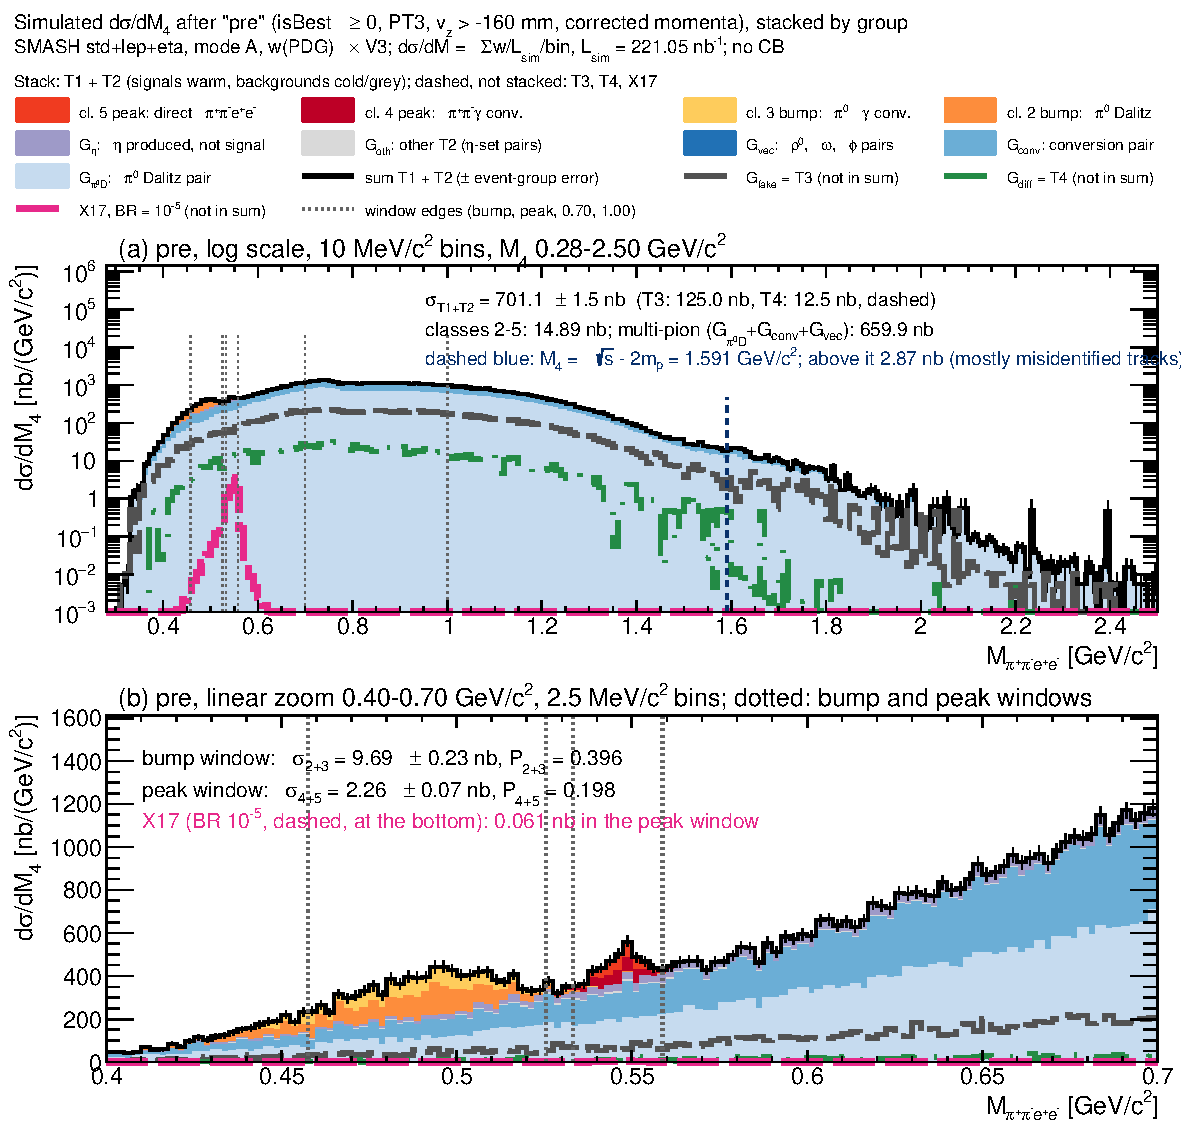
\includegraphics[width=0.68\textwidth]{figs/s5_spec_full_pre.pdf}
\caption{\textbf{What it shows: the $\eta$ peak and bump sit on a background 46 times larger.} Selection: SMASH simulation only, no combinatorial background (standard, lepton and $\eta$ sets in mode~A; PDG branching ratios $\times$ the $\eta$-decay physics weights V3); base selection ``pre'' = simulated PT3 trigger (bit 8192 set), event vertex in the target region ($z>-160$\,mm), particle identification by \betanew with the simulation polygons (pions within $3\sigma$, leptons within $5\sigma$ and with a RICH ring), energy-loss-corrected momenta of all four tracks, all stored \ppee combinations per event (isBest\,$\ge0$); no further cut; all \Mee and \Mpipi; (a) $0.28\le\Mfour<2.50$\,\GeVcc, (b) $0.40\le\Mfour<0.70$\,\GeVcc; stacked: the signal classes 2--5 and the physical background (T1+T2); windows on the simulation mass scale: peak window $0.5333\le\Mfour<0.5587$\,\GeVcc, bump window $0.4576\le\Mfour<0.5255$\,\GeVcc.
The same figure as Fig.~\ref{fig:s5full}: what the simulation predicts, $d\sigma/d\Mfour$ after ``pre'',
stacked by component; signal classes in warm colours, background groups in cold colours or grey. Dashed, not stacked:
fake leptons (T3), leptons from two sources (T4) and X17 at $\mathrm{BR} = 10^{-5}$. (a) Log scale over the full
range. (b) Linear zoom with the bump and peak windows (dotted). The $\eta$ peak and bump sit on a physical background
(mostly multi-pion) that is 46 times larger in total.}
\label{fig:res_spec}
\end{figure}

\textbf{2. The usual $\eta$ cuts do not help inside the windows.} OA$>2^\circ$, $\alpha_{\mathrm{lab}}<50^\circ$,
$\Mpipi<0.46$\,\GeVcc and $\alpha_\eta>140^\circ$ (together ``slides'') remove most of the background outside the $\eta$
windows. Inside them they remove signal about as fast as background (peak: signal $2.26\to1.37$\,nb, all counts
$11.45\to6.79$\,nb), so the purity does not rise and $F$ falls (peak $52.1\to41.0$, bump $152.7\to112.5$). Only the two
pion-vertex cuts gain inside the windows ($Q$ = 1.04--1.06). \emph{What it means:} a gain in data must come from what
the simulation lacks: the CB, or a data/SMASH difference of the multi-pion background. \emph{Status:} final; to be
checked with data. \emph{Evidence:} Fig.~\ref{fig:res_cuts}. \emph{Details:} \S\ref{sec:s5spec}, \S\ref{sec:s5cut}.
\emph{Later (Parts~II and III):} they do not help in the data either. The CB is small (CB$/N$ = 0.07--0.10 in the peak
window); OA$>2^\circ$ keeps 0.78 of the data peak and lowers the precision of its yield in every selection; once the vertex
cut is applied, the kinematic cuts add nothing; the frozen PEAK selection gains as much as the best rule tuned blind on the
data ($+1.35$ against $+1.36$ in $S/\mathrm{stat}$). After the typical cuts the simulated $\eta$ share of the peak window
hardly changes (0.298 $\to$ 0.308), and Part~III rules that they are not applied (its decision D34).

\begin{figure}[!htbp]
\centering
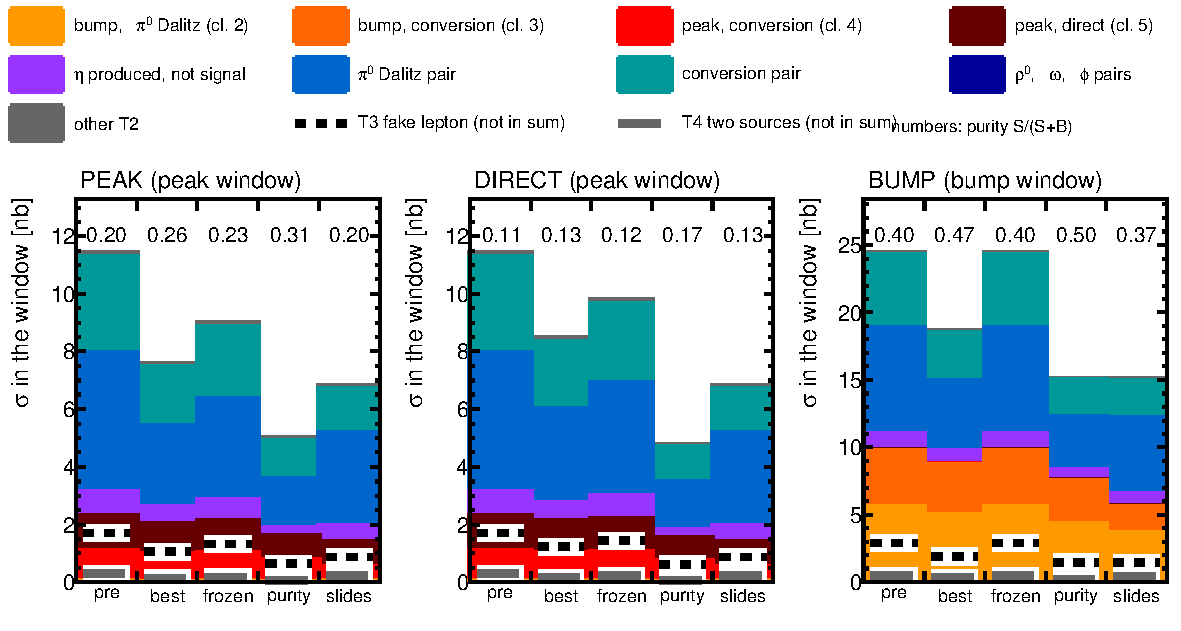
\includegraphics[width=0.80\textwidth]{figs/s5_opt_eta_composition.pdf}
\caption{\textbf{What it shows: the usual $\eta$ cuts remove signal and background alike.} The purity of the windows
therefore does not rise. Selection: SMASH simulation only, no combinatorial background (standard, lepton and $\eta$ sets in mode~A; PDG branching ratios $\times$ the $\eta$-decay physics weights V3); base selection ``pre'' = simulated PT3 trigger (bit 8192 set), event vertex in the target region ($z>-160$\,mm), particle identification by \betanew with the simulation polygons (pions within $3\sigma$, leptons within $5\sigma$ and with a RICH ring), energy-loss-corrected momenta of all four tracks, all stored \ppee combinations per event (isBest\,$\ge0$); panels: PEAK (signal classes 4+5) and DIRECT (signal class~5, class~4 counted as background) in the peak window $0.5333\le\Mfour<0.5587$\,\GeVcc, BUMP (classes 2+3) in the bump window $0.4576\le\Mfour<0.5255$\,\GeVcc; the five bars, all on top of ``pre'': ``pre'' alone; the best cell (PEAK: $0.32<\Mpipi<0.48$\,\GeVcc, $\alpha_\eta>160^\circ$, $\Delta z_\pi<40$\,mm, $\mathrm{MM}_4<2.85$\,\GeVcc; DIRECT: $0.30<\Mpipi<0.53$\,\GeVcc, $\alpha_\eta>150^\circ$, $\Delta z_\pi<40$\,mm, $\mathrm{MM}_4<2.85$\,\GeVcc; BUMP: $\alpha_{\mathrm{lab}}<70^\circ$, $0.30<\Mpipi<0.41$\,\GeVcc, $\Delta z_\pi<40$\,mm); the frozen cut (PEAK: $\Delta z_\pi<40$\,mm and $\mathrm{MM}_4<2.85$\,\GeVcc; DIRECT: $\Delta z_\pi<40$\,mm; BUMP: none); the best purity on the plateau (PEAK: $\Mpipi>0.32$\,\GeVcc, $\Delta z_\pi<40$\,mm, $\mathrm{MM}_4<2.7$\,\GeVcc; DIRECT: $\alpha_{\mathrm{lab}}<40^\circ$, $\Delta z_\pi<40$\,mm, $\mathrm{MM}_4<2.7$\,\GeVcc; BUMP: $\alpha_{\mathrm{lab}}<40^\circ$, $\Mpipi>0.32$\,\GeVcc, $\Delta z_\pi<40$\,mm); ``slides'' ($\mathrm{OA}>2^\circ$, $\alpha_{\mathrm{lab}}<50^\circ$, $\Mpipi<0.46$\,\GeVcc, $\alpha_\eta>140^\circ$). OA is the \ee opening angle, $\alpha_{\mathrm{lab}}$ the angle between the \pipi and \ee momenta in the laboratory, $\alpha_\eta$ the same angle in the rest frame of a hypothetical $\eta$, $\Delta z_\pi$ the larger distance of the two pion tracks from the event vertex along the beam and $\mathrm{MM}_4$ the missing mass of \ppee (computed with $T=4530$\,MeV). The same figure as Fig.~\ref{fig:s5optcomp}: content of the target window by group, $\sigma$ in nb, for
``pre'', the best cell, the frozen cut, the best purity on the plateau and ``slides'' (stacked: T1+T2 groups; signal
classes at the bottom in warm colours). Left: peak window (PEAK), middle: peak window, direct decay only (DIRECT),
right: bump window (BUMP). T3 (dashed line) and T4 (dash-dotted line) are drawn at their own level and are not in the
stack. Numbers above the bars: purity $S/(S+B)$, rounded; from ``pre'' to ``slides'' it goes $0.198\to0.202$ (peak) and
$0.396\to0.371$ (bump).}
\label{fig:res_cuts}
\end{figure}

\textbf{3. Frozen selections.} A rule fixed before an exhaustive scan of nine cut variables (fewest cuts within 5\,\% of
the best $F$) froze: PEAK = ``pre'' + $\Delta z_\pi<40$\,mm + $\mathrm{MM}_4<2.85$\,\GeVcc, gain in $F$ $+2.67\pm0.44$
(5.1\,\%); DIRECT = ``pre'' + $\Delta z_\pi<40$\,mm, $+1.12\pm0.10$ (4.0\,\%); BUMP = ``pre'', no cut. The optimisation
bias is below 1\,\%. \emph{Caveat:} $\Delta z_\pi$ is not yet in the compact data entries; there ``pre + both pions in the
vertex fit'' reaches $F/F_{\mathrm{best}}$ = 0.954 (PEAK). \emph{Status:} frozen on simulation without CB.
\emph{Evidence:} Fig.~\ref{fig:res_frozen}. \emph{Details:} \S\ref{sec:s5opt}.

\begin{figure}[!htbp]
\centering
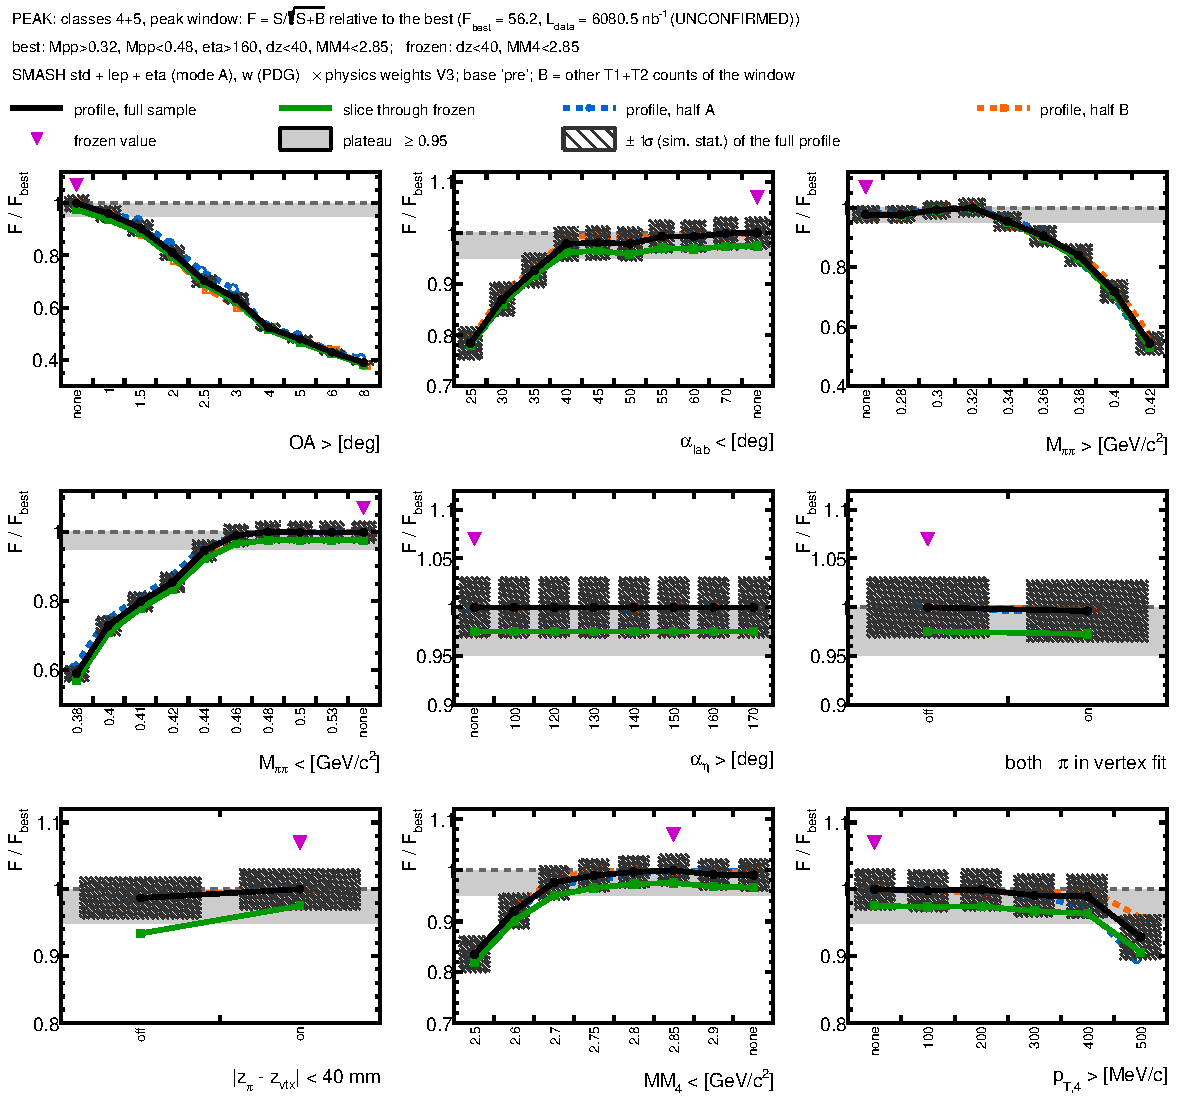
\includegraphics[width=0.66\textwidth]{figs/s5_opt_eta_profile_peak_cnt.pdf}
\caption{\textbf{What it shows: $F$ is flat; the frozen PEAK cut (triangles) sits on the plateau.} $F$ hardly depends on
the cuts. Selection: SMASH simulation only, no combinatorial background (standard, lepton and $\eta$ sets in mode~A; PDG branching ratios $\times$ the $\eta$-decay physics weights V3); base selection ``pre'' = simulated PT3 trigger (bit 8192 set), event vertex in the target region ($z>-160$\,mm), particle identification by \betanew with the simulation polygons (pions within $3\sigma$, leptons within $5\sigma$ and with a RICH ring), energy-loss-corrected momenta of all four tracks, all stored \ppee combinations per event (isBest\,$\ge0$); on top of ``pre'' the nine scanned cuts: \ee opening angle above none or 1--$8^\circ$, angle between the \pipi and \ee momenta in the laboratory below 25--$70^\circ$ or none, \Mpipi above none or 0.28--0.42\,\GeVcc and below 0.38--0.53\,\GeVcc or none, the same angle in the rest frame of a hypothetical $\eta$ above none or 100--$170^\circ$, both pions used in the event-vertex fit off or on, both pion tracks within 40\,mm of the event vertex along the beam off or on, missing mass of \ppee below 2.5--2.9\,\GeVcc or none (computed with $T=4530$\,MeV), transverse momentum of \ppee above none or 100--500\,\MeVc; signal $S$ = classes 4+5 and background $B$ = all other T1+T2 counts of the peak window $0.5333\le\Mfour<0.5587$\,\GeVcc, in expected counts at \Ldata; frozen point (PEAK): the 40\,mm pion cut and $\mathrm{MM}_4<2.85$\,\GeVcc, no other cut; halves A and B = even and odd event groups, each weighted $\times2$. The same figure as Fig.~\ref{fig:s5profile}: PEAK target, $F/F_{\mathrm{best}}$ against each of the nine cut
variables. Profile = the best $F$ over all other variables at a fixed value (full sample, black; half A and half B
relative to their own best, dashed). Hatched band: $\pm1\sigma$ statistical error of the full-sample $F$. Green: slice
through the frozen point. Grey band: plateau ($\ge0.95$). Triangle: frozen value ($\Delta z_\pi<40$\,mm,
$\mathrm{MM}_4<2.85$\,\GeVcc, no other cut; $F/F_{\mathrm{best}} = 0.975$). $\Ldata = 6080.5\,\nbinv$ (UNCONFIRMED).}
\label{fig:res_frozen}
\end{figure}

\textbf{4. Signal extraction compared with the truth.} On pseudo-data the template fit M2 recovers the peak within
$+1.4$\,\% and the calibrated Gaussian + polynomial fit M1 within $+3.1$\,\%; the side band with the simulated shape (B4)
recovers the bump within $+3.9$\,\%. Linear side bands (M3) lose 13--46\,\% of the peak (about 30\,\% on average): do not
use them. The direct decay alone comes out 20.6\,\% high (M2d), because \Mfour cannot separate it from the conversion
peak. A common simulation error of $\pm$11--15\,\% (peak) and $\pm$4.5--5\,\% (bump) must be added to every yield.
\emph{Status:} cross-check (a closure test inside one model, without CB, not blind by construction).
\emph{Evidence:} Fig.~\ref{fig:res_bias}. \emph{Details:} \S\ref{sec:s5blind}.

\emph{Later finding (Part~III), which changes the recommendation of this result} (Fig.~\ref{fig:res_stress}; details in the
note of \S\ref{sec:s5blind}). Part~III tested its estimators again on pseudo-data at the data luminosity, with a CB taken from
the data. (i) The split used here (templates from half A, truth from half B) moves the results by itself: the two halves of
the simulated background differ by 5--10\,\% per 50\,\MeVcc, four times the template noise of the real analysis. The
common simulation error of this result is this effect. (ii) With the template noise of the real analysis (truth from the
full sample, templates from bootstrap copies) every template fit comes out low: $\eta$ scale $-10$\,\%, bump $-12$\,\%,
peak $-7$\,\%. The cause is the noise of the raw simulated signal templates; a fit that scales a noisy template is pulled
towards zero. Estimators that do not scale a signal template are not biased: peak side bands $-0.5$\,\%, B4 $-1.4$\,\%.
(iii) So the template fits are only cross-checks there; the main peak estimator is a side band corrected for the leak of
the peak, with the background ratio from the smoothed simulation. (iv) The bump is measured
through the edge step B3, which closes within 2\,\% on 16\,000 pseudo-data sets. B4 is not determined in the data: its
background must be carried down 40--120\,\MeVcc from above the peak, and a quadratic term moves it by $+150$\,\%.
(v) Part~III then measured the edge in the distance to it, $u=\Mfour-E(\Mpipi,\Mee)$, where $E$ is the largest \Mfour
that the bump can reach (exact, with the \Mee term). In the simulated truth no bump count lies above its edge (largest
excess $-0.5$\,\MeVcc; without the \Mee term 3.8\,\% of class~2 would), so all edges fall on $u=0$, smeared by
6.7\,\MeVcc (Fig.~\ref{fig:res_edgeu}). The data give $0.426\pm0.020\,(\mathrm{stat})\pm0.034\,(\mathrm{syst})
\pm0.030\,(\mathrm{MC})$ of SMASH (class-2 decay angle corrected with per-count QED weights, D38; peak-tail term of D40
included), the same as the step per \Mpipi slice (0.423); $u$ is Part~III's bump measurement and the per-slice edge its
cross-check (D37). The $e^-e^-$ like-sign counts of the data also step at $u=0$; Part~III traced this to lepton pairs from the
two photons of the \piz in $\eta\to\pipi\piz$, which have exactly the bump's edge (D39; independently verified; the CB is
kept). SMASH contains such pairs, mostly $e^-e^-$ (part of them with a Compton or knock-on electron of a photon, which is
always negative); they serve only to identify the origin, since the simulation does not model the like-sign or
combinatorial background, and no like-sign rate of the data is compared with it. Charge flips of true pairs are rare
(0.01--0.04\,\% per true pair; \S\ref{sec:s5blind}, Table~\ref{tab:summarylater}). (vi) The simulated $\eta$ peak has a
low-mass tail that reaches the edge in $u$, so the step fit needs its shape; half of the simulated tail is a systematic
term (D40; result~11). D37--D40 were approved by the analyst on 15 November 2026.

\begin{figure}[!htbp]
\centering
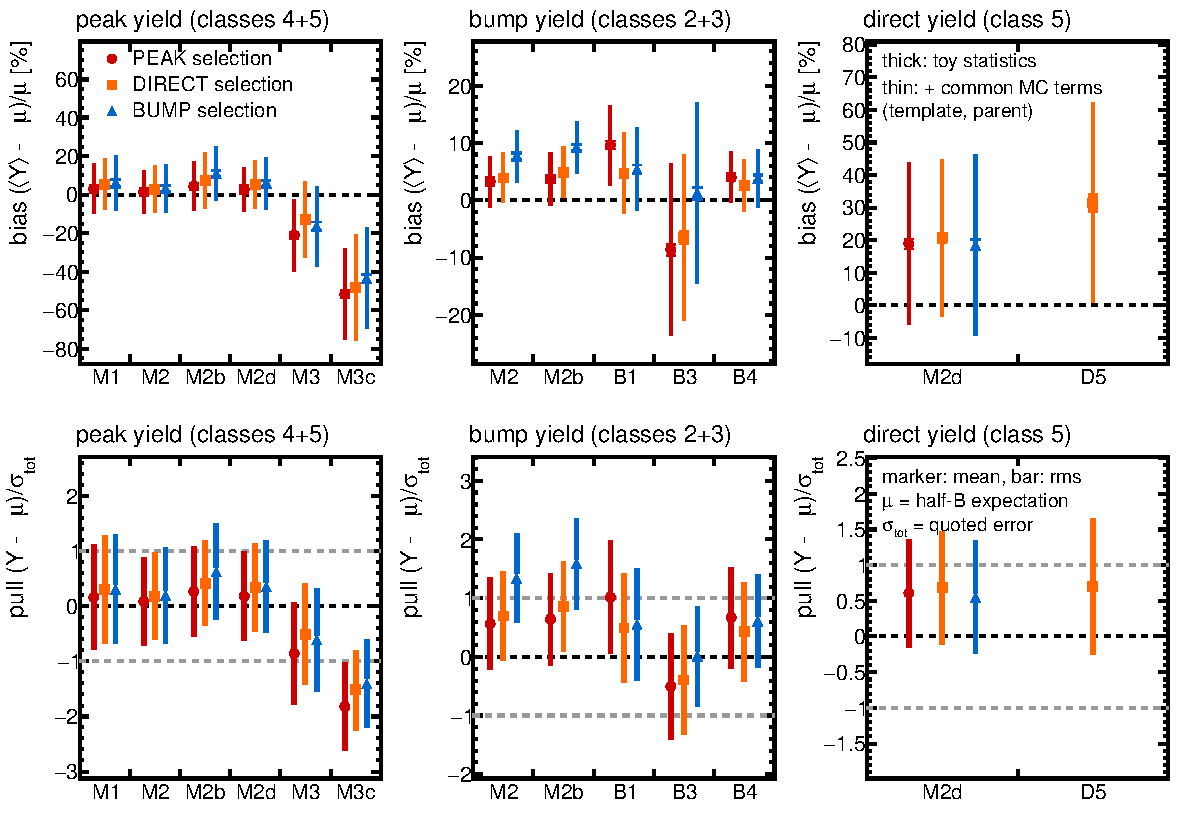
\includegraphics[width=0.68\textwidth]{figs/s5_blind_eval_eta_bias.pdf}
\caption{\textbf{What it shows: template and Gaussian fits recover the peak; linear side bands lose it.} The template
fit and the calibrated Gaussian find the true peak within a few per cent. Selection: SMASH simulation only, no combinatorial background (mode~A, weights $\times$ V3); base selection ``pre'' = simulated PT3 trigger (bit 8192 set), event vertex in the target region ($z>-160$\,mm), particle identification by \betanew with the simulation polygons (pions within $3\sigma$, leptons within $5\sigma$ and with a RICH ring), energy-loss-corrected momenta of all four tracks, all stored \ppee combinations per event (isBest\,$\ge0$); 200 pseudo-data sets at $L=110.525$\,\nbinv, pseudo-data = Poisson bootstrap of half~B (odd event groups) of the T1+T2 counts after ``pre'' with $0.30\le\Mfour<1.20$\,\GeVcc; templates from half~A (even event groups); markers for the three frozen selections: PEAK = ``pre'' plus both pion tracks within 40\,mm of the event vertex along the beam ($\Delta z_\pi<40$\,mm) and missing mass of \ppee below 2.85\,\GeVcc ($\mathrm{MM}_4$, computed with $T=4530$\,MeV); DIRECT = ``pre'' plus the 40\,mm pion cut only; BUMP = ``pre'' only; yields: peak = classes 4+5 in the peak window $0.5333\le\Mfour<0.5587$\,\GeVcc, bump = classes 2+3 in the bump window $0.4576\le\Mfour<0.5255$\,\GeVcc, direct = class~5 in the peak window ($\mu$ = their half-B expectation). D5 (shown with DIRECT) uses instead the counts of ``pre'' with both pions used in the event-vertex fit, split at $\Mee=10$\,\MeVcc. Side bands: M3 and M3c 0.5255--0.5333 and 0.5587--0.5665\,\GeVcc, B4 0.5665--0.700\,\GeVcc. The same figure as Fig.~\ref{fig:s5bias}: how well the planned methods recover the true $\eta$
yields on pseudo-data. Top: relative bias per method and selection; thick bars: toy statistics, thin bars:
including the common simulation error. Bottom: pull, marker = mean, bar = rms. Methods: M1 Gaussian + polynomial,
M2 template fit (M2b, M2d variants), M3 linear side bands (M3c with simulated curvature), B1 parametric, B3 edge
step, B4 side band with the simulated shape, D5 split in \Mee. \emph{Later (Part~III):} the fits look good here partly
because the template noise was not realistic; see Fig.~\ref{fig:res_stress}.}
\label{fig:res_bias}
\end{figure}

\begin{figure}[!htbp]
\centering
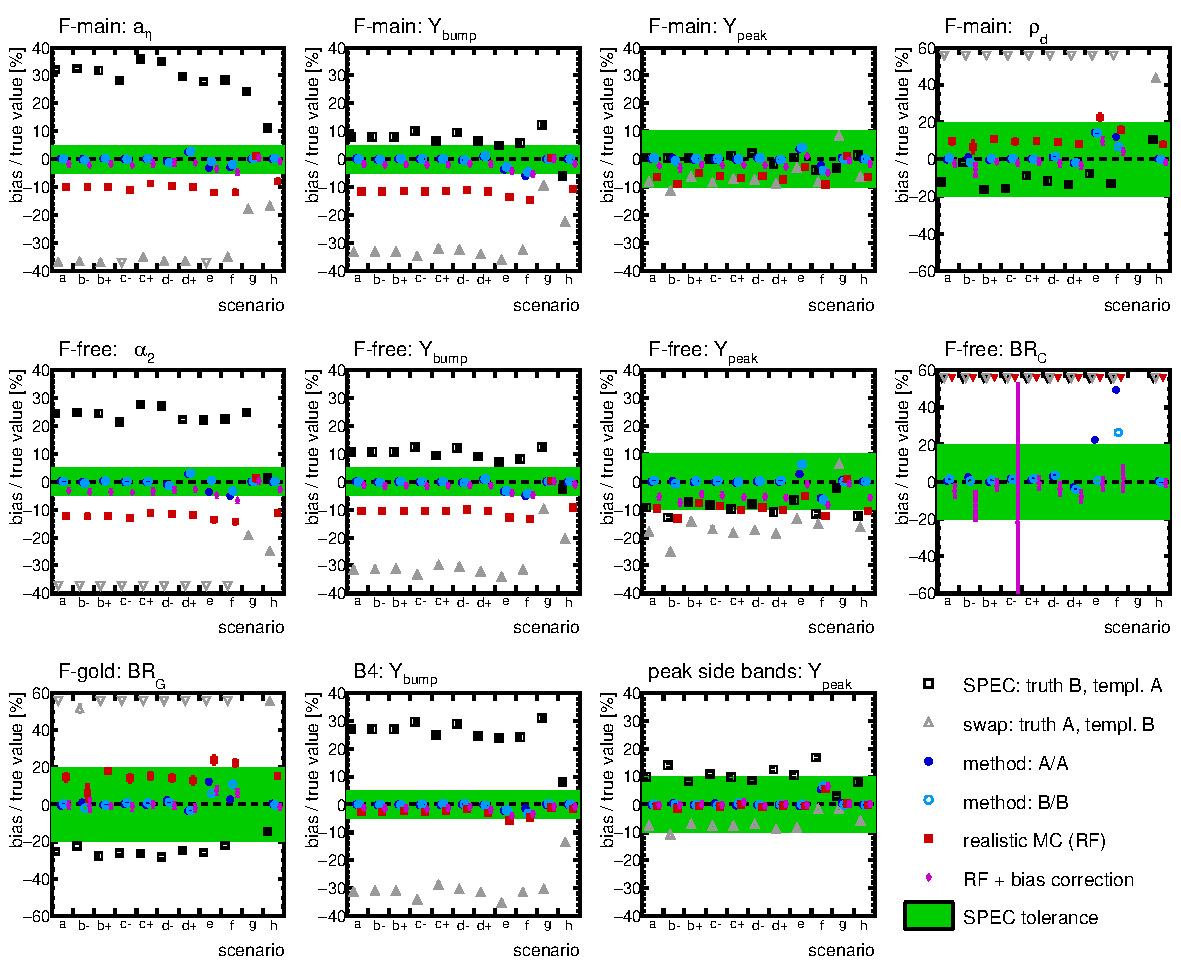
\includegraphics[width=0.84\textwidth]{figs_all/wp4_V1.pdf}
\caption{\textbf{What it shows: with the template noise of a real analysis (red squares) the template fits come out about
10\,\% low, the side bands (bottom row) do not.} Selection: pseudo-data of the Part~III selection S0, ``pre'' plus both pions used in the event-vertex fit (PT3 trigger (bit 8192 set), event vertex in the target region ($z>-160$\,mm), \betanew particle identification (pions within $3\sigma$, leptons within $5\sigma$ and with a RICH ring), corrected momenta of all four tracks, all stored combinations of each event (isBest\,$\ge0$)), at $L=6079.2$\,\nbinv; simulated part: SMASH (standard, lepton and $\eta$ sets, mode~A, weights PDG branching ratios $\times$ V3) with the masses moved to the data scale ($M_4'=0.99615\,M_4$, $\Mpipi'=0.9952\,\Mpipi$); data part: CB $=2\sqrt{N_{++}N_{--}}$ from the like-sign data ($\pi^+\pi^-e^+e^+$, $\pi^+\pi^-e^-e^-$) with the same cuts, in 10\,\MeVcc cells of \Mfour, shared out over the \Mpipi slices and \Mee classes by the like-sign share of each 50\,\MeVcc band, $k=1$. Template fits (F-main, F-free): $0.40\le\Mfour<0.70$\,\GeVcc in the five \Mpipi slices below 0.34, 0.34--0.37, 0.37--0.39, 0.39--0.43 and above 0.43\,\GeVcc, each split into $\Mee<10$ and $\Mee\ge10$\,\MeVcc; F-gold: the same slices with $\Mee\ge20$\,\MeVcc only; B4: bump window $0.4550\le\Mfour<0.5225$\,\GeVcc, background carried down from $0.565\le\Mfour<0.700$\,\GeVcc, all \Mee and \Mpipi; peak side bands: peak window $0.53364\le\Mfour<0.55416$\,\GeVcc, side bands $0.5250$--$0.5336$ and $0.5542$--$0.5628$\,\GeVcc, all \Mee and \Mpipi. Later finding of Part~III (its Fig.~V1, \code{report_all.pdf}; file
\code{figs_all/wp4_V1.pdf}): relative bias of each estimated quantity in the truth scenarios (a)--(h) of its stress test,
500 pseudo-data sets per point at the data luminosity, 6079.2\,\nbinv. The truth is the smoothed simulated non-$\eta$
background plus the simulated $\eta$ classes plus a CB built from the like-sign pairs of the \emph{data} (selection ``pre''
+ both pions in the vertex fit), so this is not a simulation-only figure. Open squares: truth from half B, templates from
half A, as in the blind test of this report; open triangles: the swap; full and open circles: truth and templates from the
same half; red squares: truth from the full sample, templates from bootstrap copies (the template noise of the real
analysis); magenta diamonds: red squares with a bias correction. Green band: tolerance. F-main, F-free, F-gold: template
fits ($a_\eta$: $\eta$ scale; $Y$: yields; $\rho_d$, $\alpha_2$, BR: other fit parameters); B4: bump side band with the
simulated shape; peak side bands: corrected for the leak of the peak. Triangles at the frame: outside the range.}
\label{fig:res_stress}
\end{figure}

\begin{figure}[!htbp]
\centering
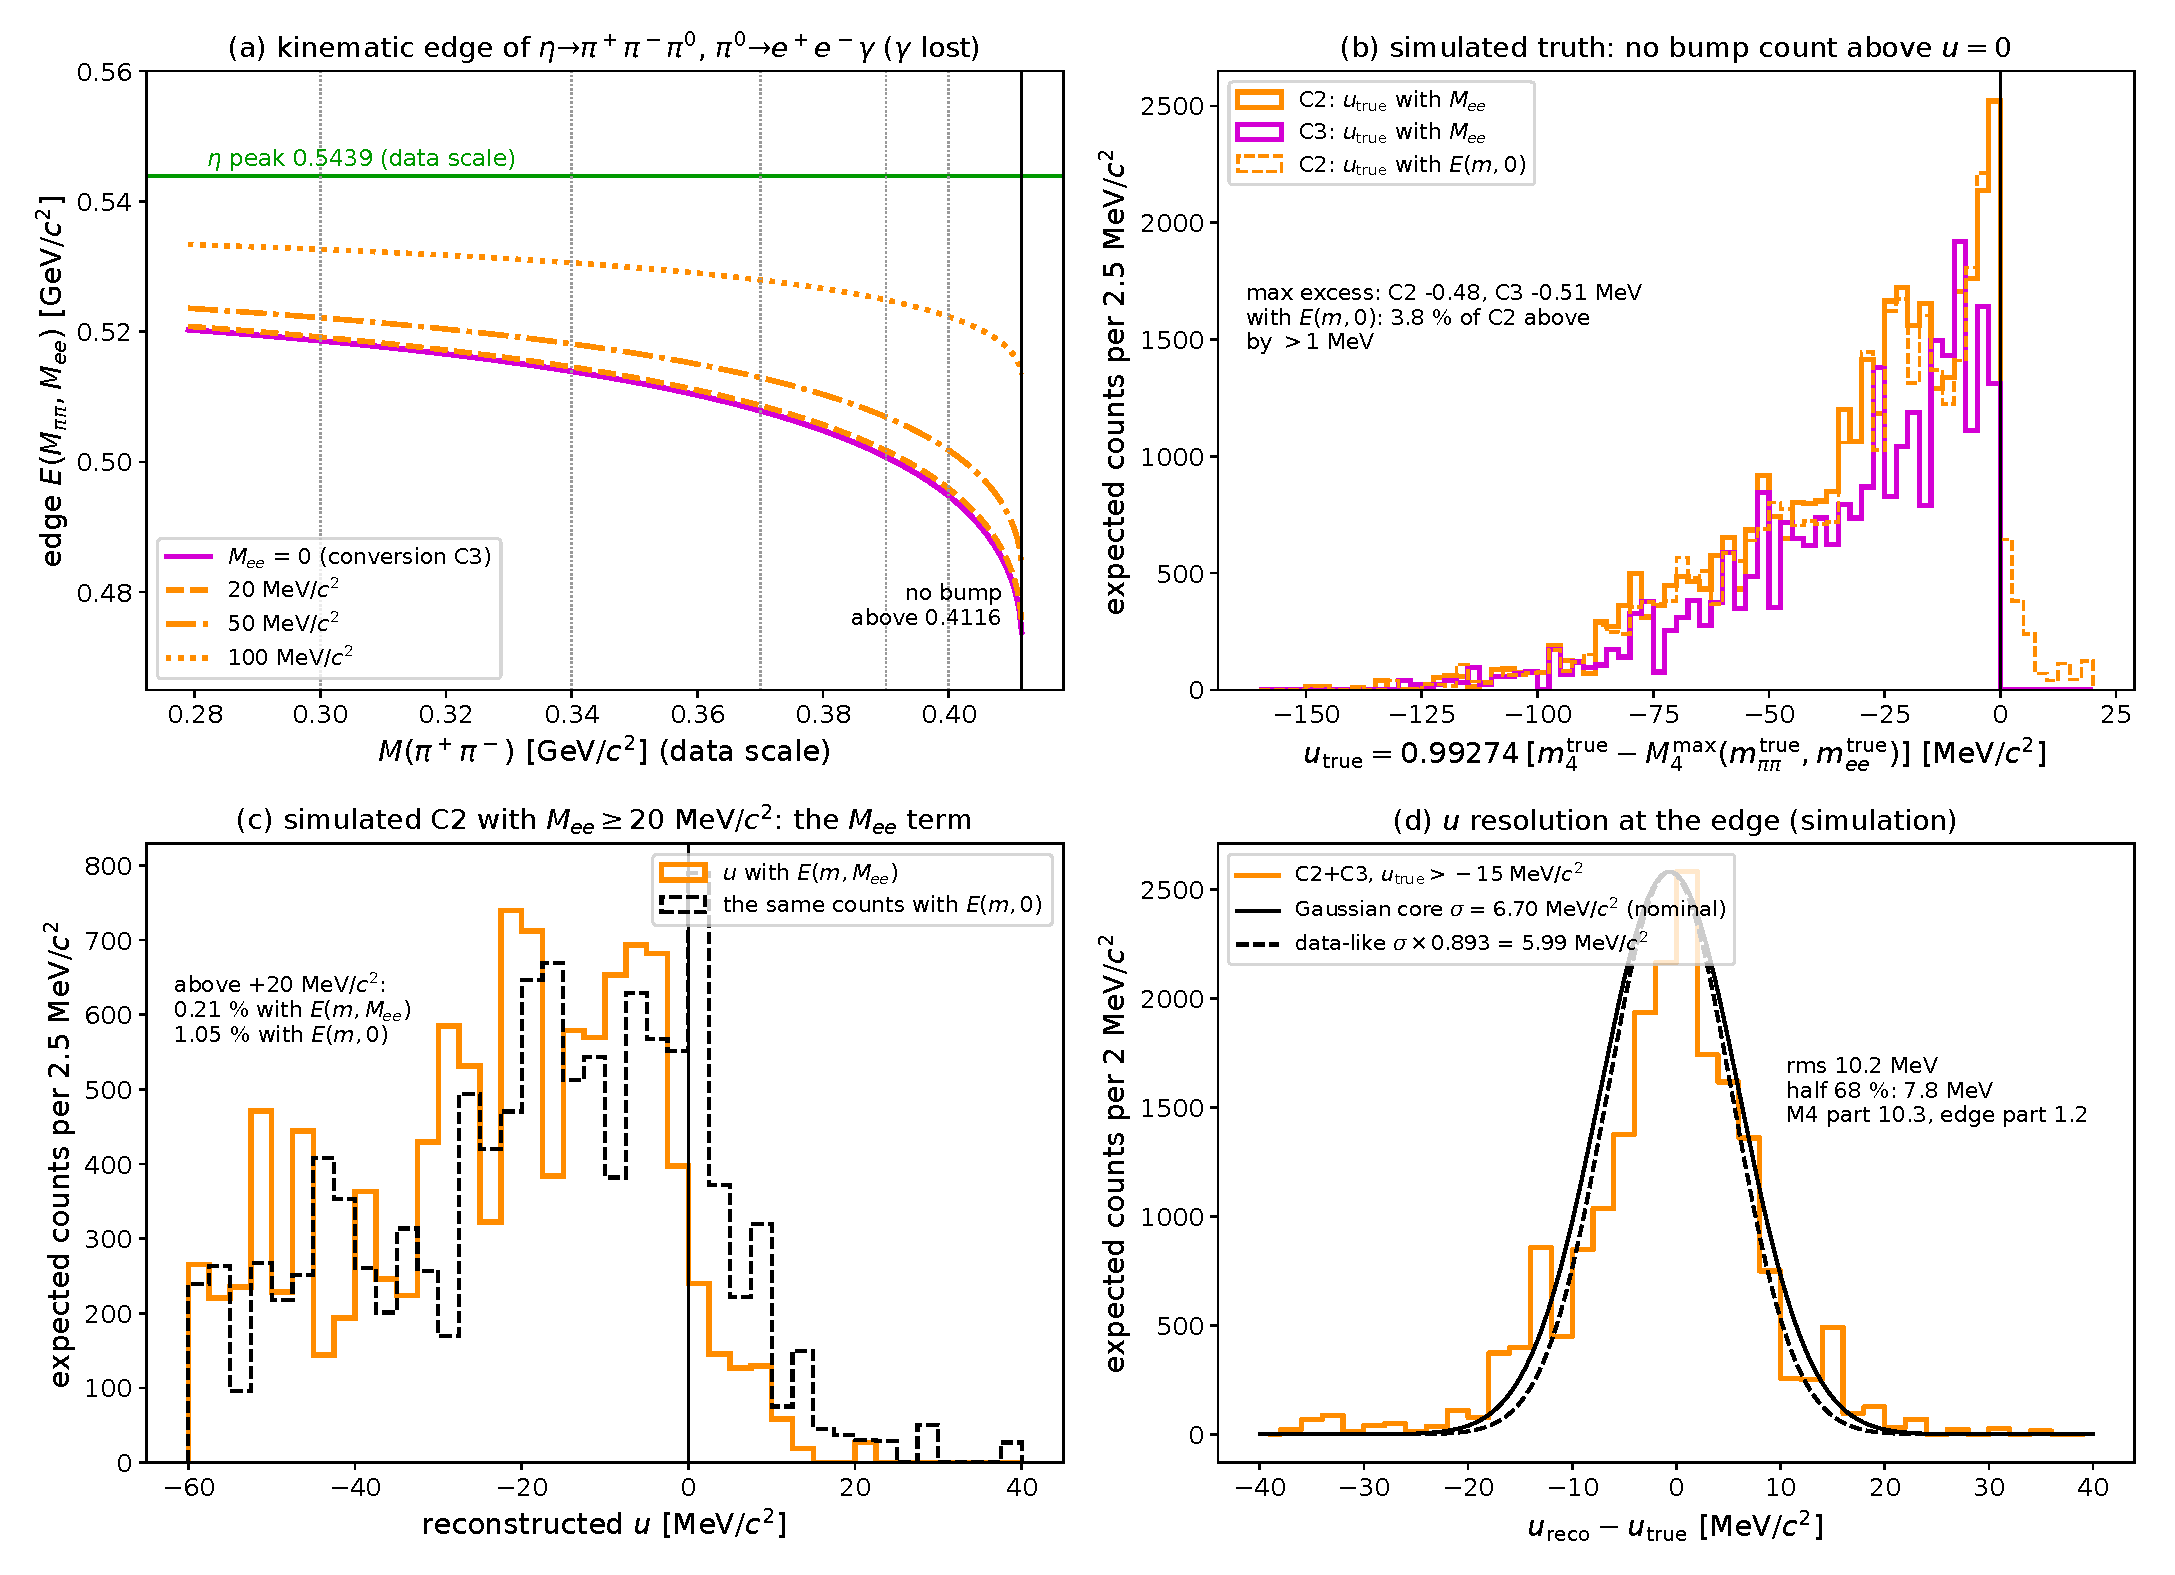
\includegraphics[width=0.84\textwidth]{figs_all/edgeu_kinematics_cnt.pdf}
\caption{\textbf{What it shows: once the edge of the bump is computed with both \Mpipi and \Mee, no simulated bump count
lies above it, so in the distance to it, $u$, all bump counts end at $u=0$, smeared by 6.7\,\MeVcc.} Selection: SMASH simulation only (mode~A, weights PDG branching ratios $\times$ V3, no QED angle correction of class~2); Part~III's ``pre'' plus the pion-vertex cut = simulated PT3 trigger (bit 8192 set), event vertex in the target region ($z>-160$\,mm), \betanew particle identification (pions within $3\sigma$, leptons within $5\sigma$ and with a RICH ring), corrected momenta of all four tracks, all stored combinations of each event (isBest\,$\ge0$), both pions used in the event-vertex fit; masses on the data scale of Part~III, $M_4'=0.99615\,M_4$, $\Mpipi'=0.9952\,\Mpipi$; expected raw counts at 6079.2\,\nbinv; (a) the edge function only, no counts; (b)--(d) classes 2 and 3 with $0.30\le\Mpipi'<0.40$\,\GeVcc; (c) class~2 with reconstructed $20\le\Mee<135$\,\MeVcc ($u$ is not defined above the \piz mass); (d) classes 2+3 with $u_{\mathrm{true}}>-15$\,\MeVcc and reconstructed $\Mee<135$\,\MeVcc. Later finding of
Part~III (result~4 (v)); simulation only. The same figure as Fig.~\ref{fig:s5edgeu}, where the caption gives every
detail. (a) The edge $E(\Mpipi,\Mee)$ for four values of \Mee. (b) True $u$ of class~2 (orange) and class~3 (magenta);
dashed: class~2 with the edge at $\Mee=0$, which puts counts above $u=0$. (c) Reconstructed $u$ of class~2 with
$\Mee\ge20$\,\MeVcc, with and without the \Mee term. (d) Reconstructed minus true $u$ near the edge: width 6.7\,\MeVcc.}
\label{fig:res_edgeu}
\end{figure}

\textbf{5. X17: expected sensitivity.} With the X17 selection (peak window, $15.5\le\Mee<24.5$\,\MeVcc, both pions in
the vertex fit) the expected 90\,\% CL upper limit on $\mathrm{BR}(\eta\to\pipi X17)\,\mathrm{BR}(X17\to\ee)$ is
$1.9\times10^{-5}$; it would be $5.7\times10^{-6}$ with the background known exactly. The limit is set by the
simulation statistics of the background: one standard-set entry stands for 27.5 data counts. \emph{Status:} expected,
PRELIMINARY (\Ldata unconfirmed, no CB, SMASH background, phase space and isotropic decay assumed for X17).
\emph{Evidence:} Fig.~\ref{fig:res_x17}. \emph{Details:} \S\ref{sec:s5x17}, \S\ref{sec:s5blind}.
\emph{Later (Part~III):} the search was done in the data with a frozen fit of $\Mfour\times\Mee$ in which the background is
measured in every \Mee bin from the \Mfour side bands, as decision~2 of \S\ref{sec:resdec} asked. The observed 90\,\%
CL$_s$ limit at 17\,\MeVcc is $r<0.114$ times BR$(\eta\to\ppee)$, i.e.\ $3.16\times10^{-5}$ with the PDG 2026 value
$2.76\times10^{-4}$ (the analyst ruled on 15 November 2026 that PDG 2026 is used everywhere, D25)\footnote{\label{fn:x17pdg}With the PDG 2020
value BR$(\eta\to\ppee)=(2.68\pm0.11)\times10^{-4}$, which the frozen procedure fixed before the unblinding, the same limit
$r<0.114$ reads $\mathrm{BR}(\eta\to\pipi X17)\,\mathrm{BR}(X17\to\ee)<3.06\times10^{-5}$.}; the expected one is
$2.68\times10^{-5}$ (68\,\% band 1.54--4.92). The
$1.9\times10^{-5}$ of this result is not like-for-like: it assumed that the data hold all the $\eta$ that SMASH predicts
(they hold about 0.4) and used a counting window. Part~III also finds that two thirds of the simulated X17 pairs have
OA$<6^\circ$ and that every usual cut acts on X17 as on the direct decays within 5\,\% (Fig.~\ref{fig:s5x17oa}).

\begin{figure}[!htbp]
\centering
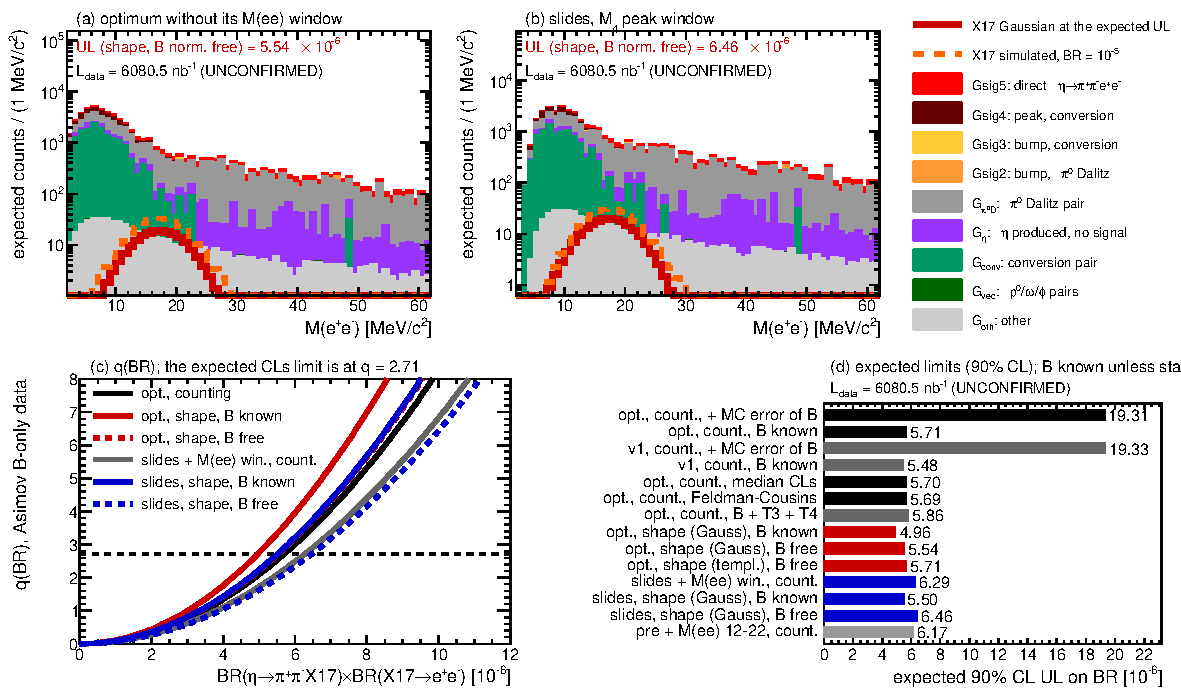
\includegraphics[width=0.80\textwidth]{figs/s5_opt_x17_shape_cnt.pdf}
\caption{\textbf{What it shows: the X17 limit is set by the simulation error of the background.} It is not set by the
statistics of the data. Selection: SMASH simulation only, no combinatorial background (standard, lepton and $\eta$ sets in mode~A; PDG branching ratios $\times$ the $\eta$-decay physics weights V3); base selection ``pre'' = simulated PT3 trigger (bit 8192 set), event vertex in the target region ($z>-160$\,mm), particle identification by \betanew with the simulation polygons (pions within $3\sigma$, leptons within $5\sigma$ and with a RICH ring), energy-loss-corrected momenta of all four tracks, all stored \ppee combinations per event (isBest\,$\ge0$); all panels inside the peak window $0.5333\le\Mfour<0.5587$\,\GeVcc; (a) the frozen X17 selection v2 without its \Mee window: ``pre'' plus both pions used in the event-vertex fit, \Mee 2--62\,\MeVcc in 1\,\MeVcc bins (the frozen window $15.5\le\Mee<24.5$\,\MeVcc is not applied); (b) ``pre'' plus the four ``slides'' cuts instead of the pion-vertex cut: $\mathrm{OA}>2^\circ$ (\ee opening angle), $\alpha_{\mathrm{lab}}<50^\circ$ (angle between the \pipi and \ee momenta in the laboratory), $\Mpipi<0.46$\,\GeVcc and $\alpha_\eta>140^\circ$ (the same angle in the rest frame of a hypothetical $\eta$); \Mee 2--62\,\MeVcc; (c) and (d): the shape fits use \Mee 2--62\,\MeVcc, the counting limits $15.5\le\Mee<24.5$\,\MeVcc; ``opt.'' = v2, ``v1'' = $0.5330\le\Mfour<0.5555$\,\GeVcc, $13.0\le\Mee<26.5$\,\MeVcc and pions in the vertex fit, ``pre + M(ee) 12--22'' = peak window and $12\le\Mee<22$\,\MeVcc only; background $B$ = T1 without X17 plus T2 (one entry adds T3 and T4). The same figure as Fig.~\ref{fig:s5x17shape}: X17 search, expected counts at $\Ldata = 6080.5\,\nbinv$
(UNCONFIRMED). (a) \Mee at the v2 optimum without its \Mee window, stacked background groups, X17 as a Gaussian at the
expected limit of the shape fit and as the simulated template at $\mathrm{BR}=10^{-5}$. (b) The same for ``slides''.
(c) Test statistic $q(\mathrm{BR})$ on Asimov background-only data; the expected CLs limit is at $q = 2.71$.
(d) Expected 90\,\% CL limits in units of $10^{-6}$; ``B known'' ignores the MC error of $B$. The top two bars are the
$1.9\times10^{-5}$ (with the MC error of $B$) and $5.7\times10^{-6}$ (background known exactly) of the text.}
\label{fig:res_x17}
\end{figure}

\textbf{6. Defects of the simulation chain, found and corrected.} The HGeant card sets $\mathrm{BR}(\eta\to\ee\gamma)$ to
6.0\,\% instead of the default 0.60\,\% (normalised 6.04\,\%, 8.8 times the PDG value 0.69\,\%); the generator's
$\eta\to\ppee$ has no virtual photon (4.7\,\% of the pairs above 20\,\MeVcc instead of 28\,\%). Weights correct both;
smaller defects are corrected in the code. One tension remains: OA$>2^\circ$ keeps $0.697\pm0.015$ of the simulated
peak (0.59 before the weights) against $0.778\pm0.033$ in the data. \emph{Status:} final; the producers must confirm
the HGeant setting; the data values were measured outside Part~I (Table~\ref{tab:summary}, note b).
\emph{Later (Parts~II and III):} Part~II's final data values are $0.772\pm0.037$ for OA$>2^\circ$ (side bands; 0.778 from
the ratio of fitted peak contents) and $0.23\pm0.04\,(\mathrm{stat})\pm0.05\,(\mathrm{method})$ for the share above
$\Mee=20$\,\MeVcc. The share agrees with the simulated 0.219, so that tension is gone; the OA tension stays
($1.9\sigma$). Part~III, with the simulated shapes, finds relatively fewer close (conversion) pairs in the data than in
SMASH: the conversion route gives $0.24\pm0.05$ of SMASH, the direct decays $0.50\pm0.06$, and the data peak has a share
$0.546\pm0.053$ above $\Mee=10$\,\MeVcc against 0.425 in SMASH ($2.3\sigma$). This points the same way as the OA tension.
The cause (close-pair efficiency, simulated material or the rate of the direct decay) is open. The analyst ruled on
15 November 2026 (Part~III, D32) that it stays to be tested in a separate analysis: the reconstruction efficiency of \ee
pairs with opening angle 0--$6^\circ$ in data and simulation, from \piz, $\eta$ and $\omega$ Dalitz decays with the \ee
hypothesis plus the ECAL photon; it waits for the trigger-bias correction and the new ECAL calibration. Until then
Part~III takes the make-up of the $\eta$ peak from the data (D31, ruled, provisional): if the test shows that the data lose
close pairs, its direct-decay route (0.52\,mb) becomes the natural headline, with a much smaller composition term; if not,
the two routes must differ through the simulated material or the rate of the direct decay, and 0.43\,mb with a $\pm32$\,\%
composition term stays.
\emph{Evidence:} Fig.~\ref{fig:res_gen}, left and middle (the generator of the direct decay; the HGeant branching ratios and the rounded
codes are tables: Tables~\ref{tab:hgeant} and~\ref{tab:float}). \emph{Details:} Appendix~\ref{sec:tech}.

\begin{figure}[!htbp]
\centering
\begin{minipage}[b]{0.355\textwidth}\centering
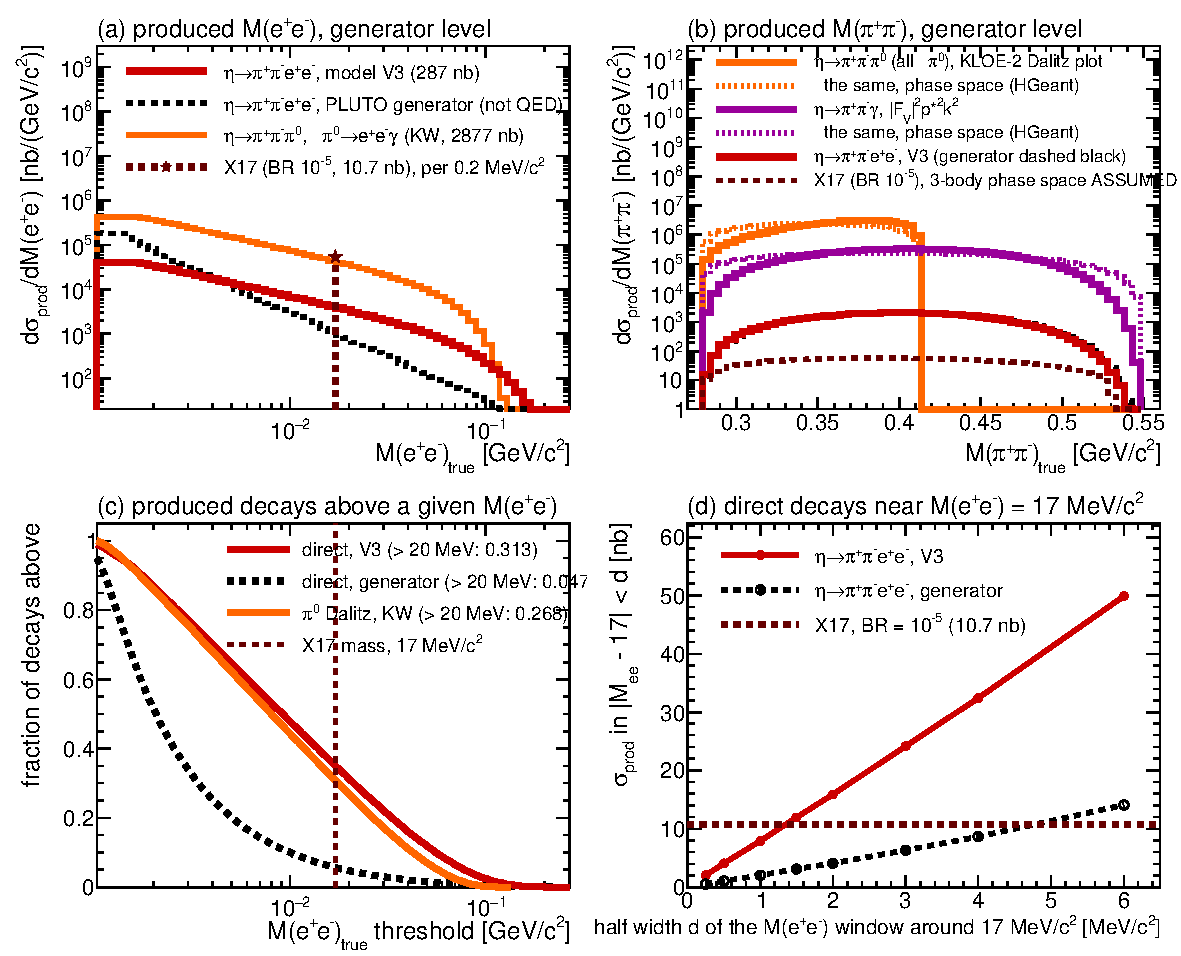
\includegraphics[width=\textwidth,trim=0 228 284 0,clip]{figs/s5_acc_gen.pdf}
\end{minipage}\hfill
\begin{minipage}[b]{0.355\textwidth}\centering
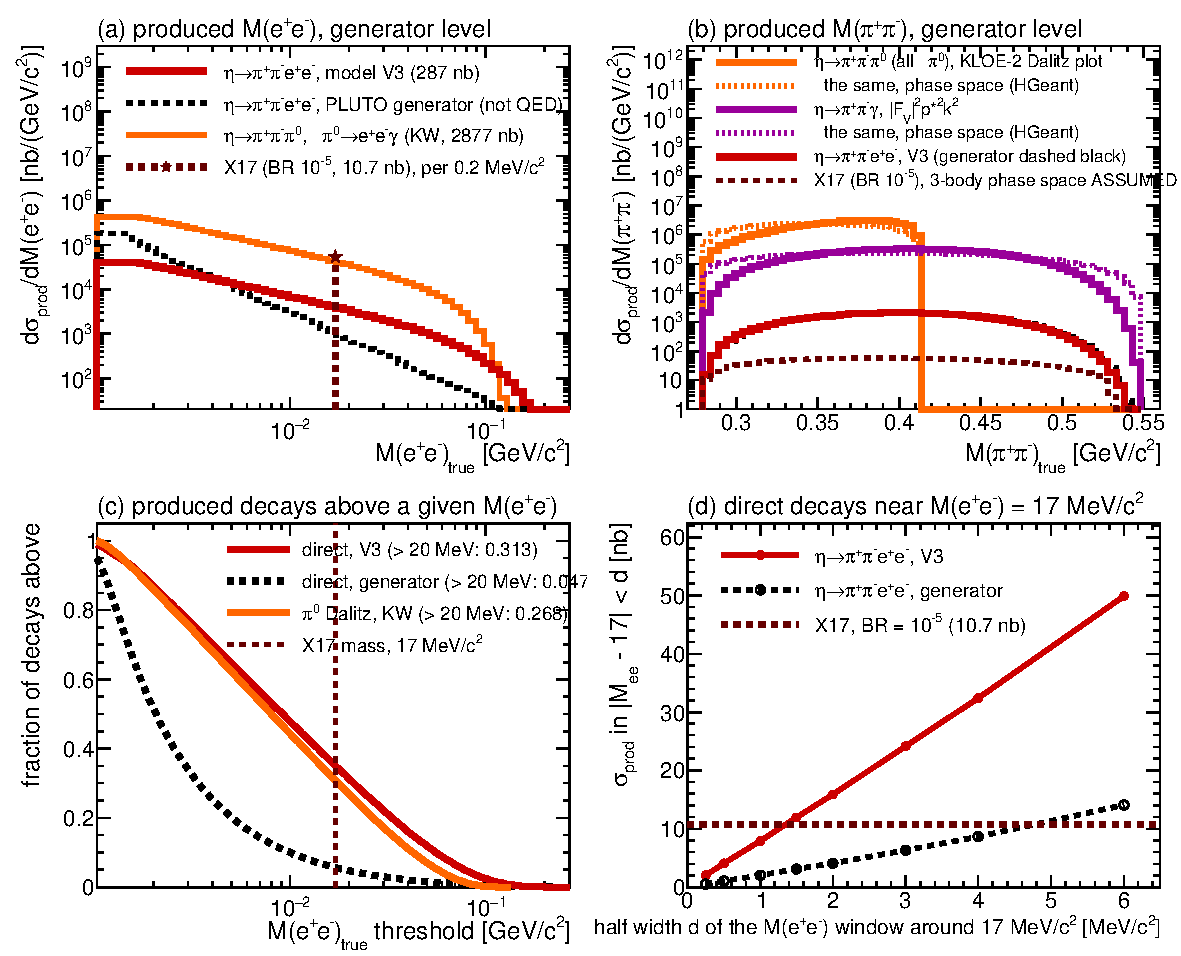
\includegraphics[width=\textwidth,trim=0 0 284 231,clip]{figs/s5_acc_gen.pdf}
\end{minipage}\hfill
\begin{minipage}[b]{0.255\textwidth}\centering
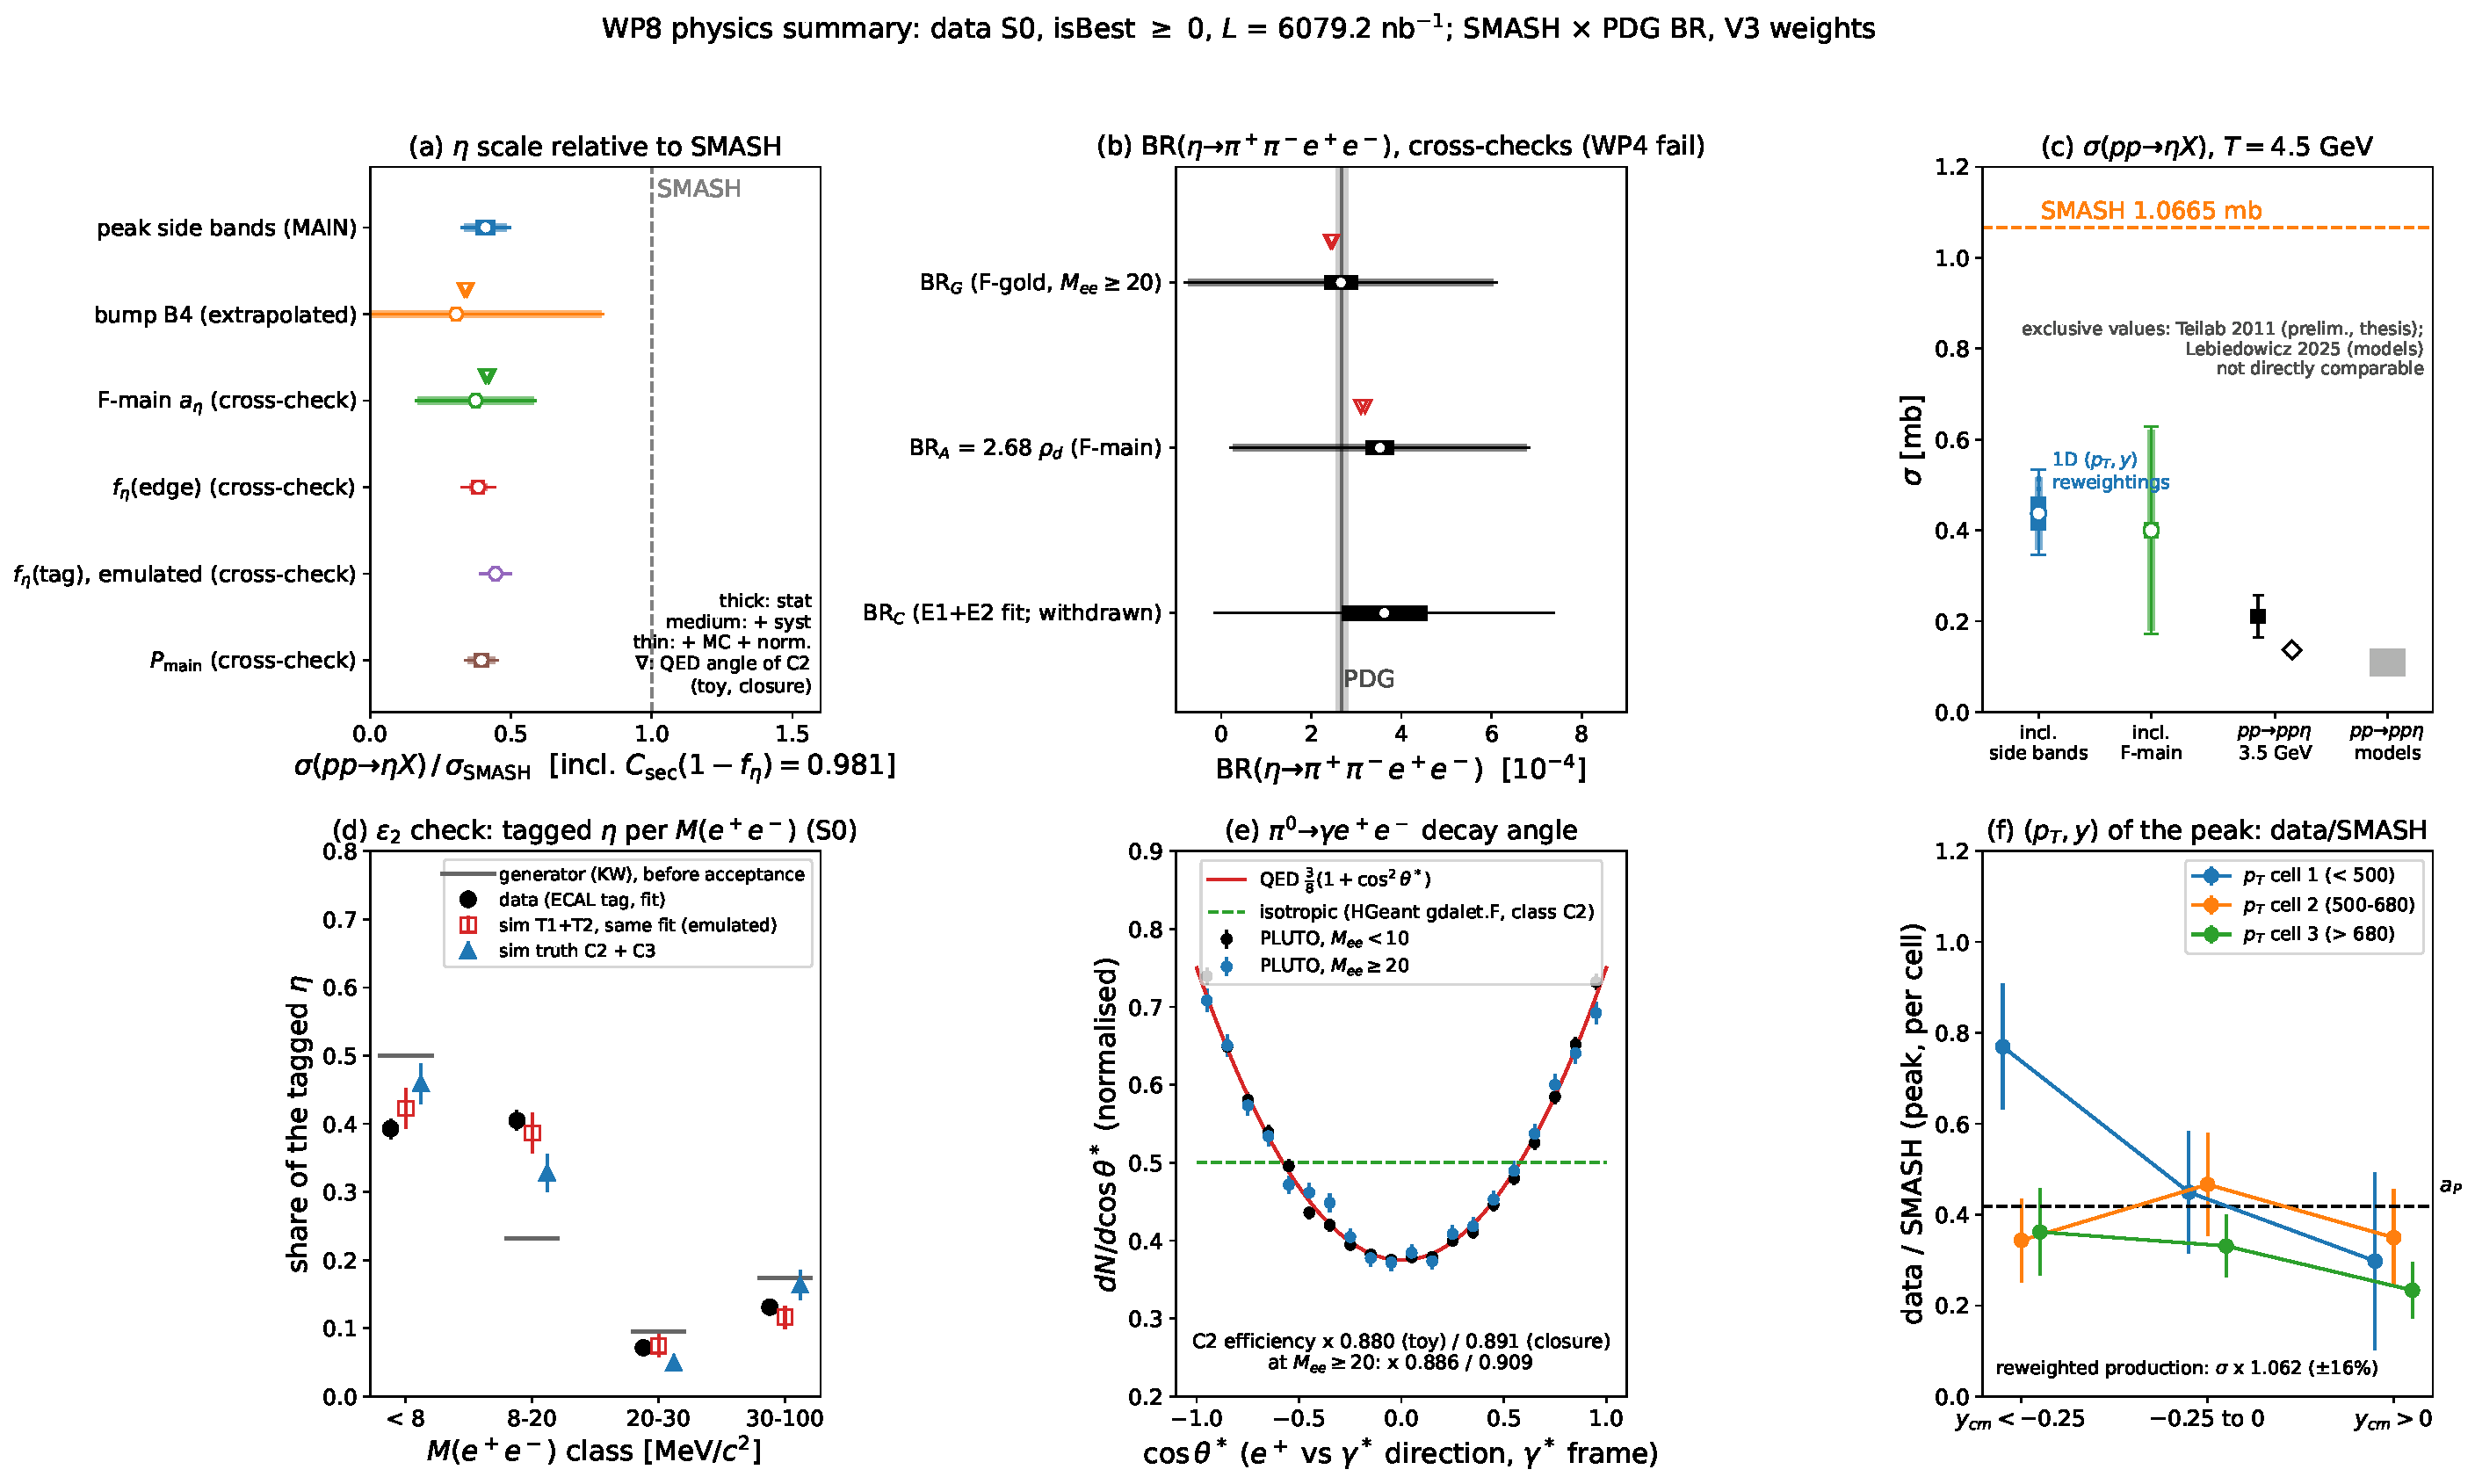
\includegraphics[width=\textwidth,trim=594 5 447 437,clip]{figs_all/wp8_P1.pdf}
\end{minipage}
\caption{\textbf{What it shows: two wrong decay distributions, one fixed here, one found later.} Selection: none in any panel: generator level, before the detector simulation, without any cut or acceptance. Left and middle: the direct decays from the PLUTO generator sample of the $\eta$ set (1\,181\,801 decays in 1000 of the 100\,000 files), with the physics weights V3 and as generated; the \piz Dalitz pair of the bump from its production density (Kroll--Wada); the X17 line at 17\,\MeVcc. Right: the \piz Dalitz decays of PLUTO in the lepton set (124\,k decays) with $\Mee<10$\,\MeVcc and with $\Mee\ge20$\,\MeVcc, against the QED formula and the isotropic decay of the HGeant source code (no simulated counts).
Left and middle (result~6, corrected here): the generator's $\eta\to\ppee$ lacks large \Mee; the physics weights V3 restore it. Panels (a)
and (c) of Fig.~\ref{fig:s5gen}, generator level, before acceptance. Left (a): produced \Mee of the direct decay with the
physics weights (V3, solid red) and in the PLUTO generator (not QED, dotted black), of the \piz Dalitz pair of the bump
(Kroll--Wada) and the X17 line. Middle (c): fraction of the produced decays above a given \Mee; above 20\,\MeVcc it is
0.047 in the generator, 0.313 with V3 and 0.268 for the \piz Dalitz pair (28\,\% for Kroll--Wada with phase space only,
as in the text). Right (result~7, found later in Part~III): HGeant decays the virtual photon $\gamma^*$ of $\piz\to\ee\gamma$ isotropically (flat
green line); QED and PLUTO give $1+\cos^2\theta^*$. Panel (e) of the Part~III summary figure (\code{report_all.pdf}, file
\code{figs_all/wp8_P1.pdf}): distribution of $\cos\theta^*$, the emission angle of the $e^+$ in the rest frame of the
$\gamma^*$, for the \piz Dalitz decays of PLUTO (lepton set, two \Mee classes, points) against QED
$(3/8)(1+\cos^2\theta^*)$ (red line) and the isotropic decay of HGeant (class~2, standard set). The factors printed in
the panel ($\times0.880$ from a toy, $\times0.891$ from the closure) are the class-2 efficiency with the QED angle divided by
that with the isotropic angle: 12--14\,\%, which explains the lepton/standard closure $0.891\pm0.003$ of prompt \piz Dalitz
pairs. For the bump the full simulation gives 0.86: the simulated class-2 efficiency of the bump is about 16\,\% too high
(result~7).}
\label{fig:res_gen}\label{fig:res_qed}
\end{figure}

\textbf{7. Closure between the sets, and its later explanation.} The same physics taken from two sets should give the
same yield: counts without a forced $\eta$ agree to $1.0056\pm0.0036$, but the Dalitz pairs do not (lepton/standard
$0.891\pm0.003$ for \piz, $0.879\pm0.005$ for $\eta$). \emph{Later finding (Part~III):} HGeant decays the virtual photon
$\gamma^*$ of the \piz Dalitz decay isotropically instead of as $1+\cos^2\theta^*$, so the simulated efficiency of
class~2 is too high: by 12--14\,\% in the toys and for the prompt \piz Dalitz pairs of the closure, which explains 0.891.
\emph{Later (Part~III, C2 factor reconciliation):} weighting every simulated class-2 count with the QED angle, averaged
over the circle on which its lost photon must lie, gives the factor 0.86 for the bump edge (0.864 over all \Mfour), i.e.\
the simulated efficiency of the bump is about 16\,\% too high; the toys (0.88) had too many soft leptons, and the closure
0.891 comes from prompt \piz Dalitz pairs with another selection (\S\ref{sec:weights}). Not corrected here. Part~III applies
these per-count QED weights to its bump-edge results (its D38, approved by the analyst on 15 November 2026, until a future
simulation corrects the angle in GEANT itself, which is not expected). \emph{Status:} cross-check; the correction is
applied in Part~III (\code{report_all.pdf}, section ``Efficiencies and the QED check of the bump simulation'').
\emph{Evidence:} Fig.~\ref{fig:res_qed}, right. \emph{Details:} \S\ref{sec:weights}.



\textbf{8. Particle identification.} The PID cuts (momentum against $\betanew$, a velocity from the relative times of
flight) differ little between simulation (v6) and data (v1); PID efficiencies come from complete combinations, because
$\betanew$ depends on the partner tracks. Electrons without a RICH ring make 2.5\,\% of the \pim slot; a cut on the MDC
energy loss at 2.2 reduces them to 0.4\,\%, but keeps only 79\,\% of the pions below 300\,\MeVc. \emph{Status:} final
for the simulation; the energy loss was not yet checked in data. \emph{Evidence:} Fig.~\ref{fig:res_pid} (the electrons
in the \pim slot: Fig.~\ref{fig:pimslot}). \emph{Details:} \S\ref{sec:pid}.

\begin{figure}[!htbp]
\centering
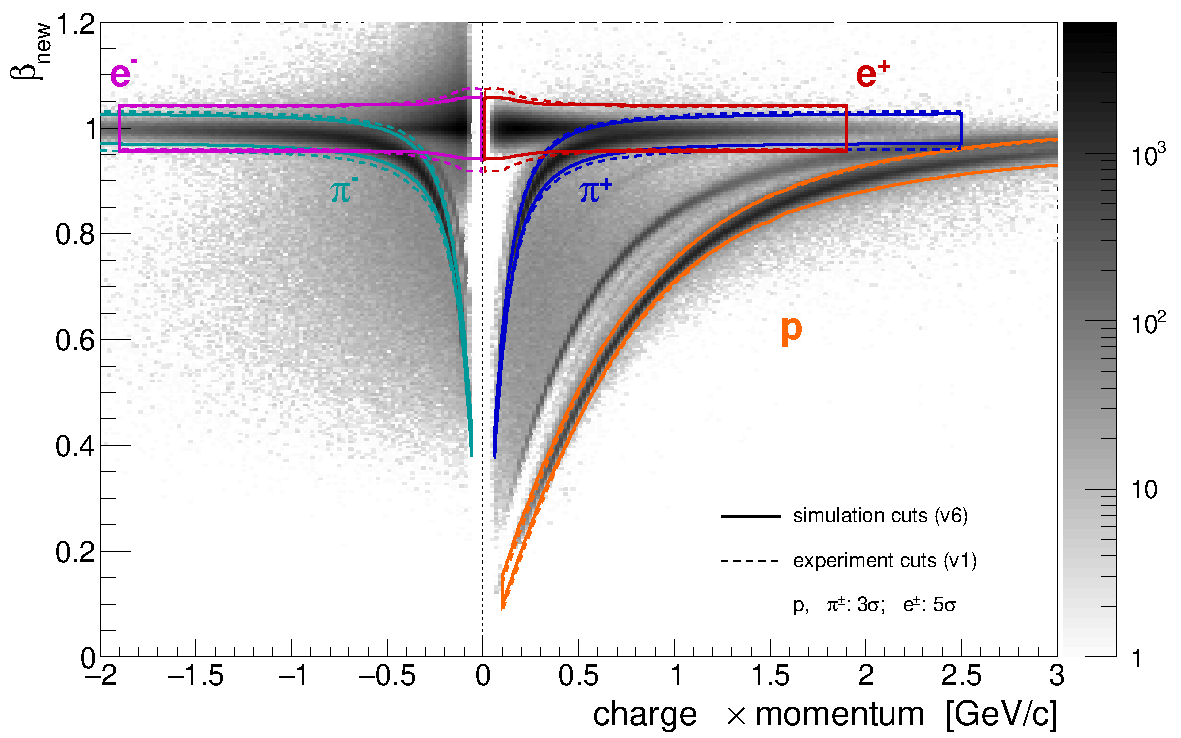
\includegraphics[width=0.50\textwidth]{figs/banana_all.pdf}
\caption{\textbf{What it shows: the simulation (solid) and experiment (dashed) PID cuts differ little.} Selection: simulated tracks of SMASH p+p at 4.5\,GeV before the PID cut; only the best-ranked combination of each event (isBest\,$=1$); a reconstructed event vertex ($z>-500$\,mm); no trigger condition, no target-region cut, unweighted; protons and pions: all tracks of the p, \pip and \pim slots of the hypothesis p\pip\pim (hadron PID sample \code{HH_elossfix}, 150 of 1000 files); $e^\pm$: all tracks of the $e^+$ and $e^-$ slots of the lepton PID sample (\code{LEP_merged}, 101 files), hypothesis \ppee, whose lepton slots hold only tracks with a correlated RICH ring and whose pion slots hold tracks without one.
The same figure as Fig.~\ref{fig:banana}: $\betanew$ versus charge times momentum for simulated tracks before the PID
cut (SMASH p+p at 4.5\,GeV, no trigger condition, $\mathrm{isBest}=1$, vertex $z>-500$\,mm); protons and pions from the
hadron PID sample, $e^\pm$ from the lepton PID sample. Solid lines: simulation cuts (v6), dashed: experiment cuts (v1);
p and $\pi^\pm$ at $3\sigma$, $e^\pm$ at $5\sigma$.}
\label{fig:res_pid}
\end{figure}

\textbf{9. Samples and normalisation.} Three sets of the same $10^{10}$ SMASH collisions (natural decays; dilepton
decays forced; $\eta$ decays forced), each worth $\Lsim = 221.05\,\nbinv$; a physical weight $W$ on every count makes them
addable ($\sum W/\Lsim$ is a cross section). One unit of $\sum W$ stands for 27.51 data counts, so the 1\,649 simulated
entries of the bump with a \piz Dalitz pair stand for 42\,900 data counts. \emph{Status:} final for \Lsim; 27.51
preliminary (it depends on \Ldata). \emph{Evidence:} no figure needed (luminosities and weights; Tables~\ref{tab:sets},
\ref{tab:norm} and~\ref{tab:fat}). \emph{Details:} \S\ref{sec:samples}.

\textbf{10. Later finding (Part~III): the ECAL and the lost photon of the bump.} \emph{In short:} one third of the lost
bump photons hit an active ECAL module, but they are soft, so only about one bump count in ten is fully reconstructed in the
simulation. \emph{What was done:} the simulation does not store the lost photon of a bump combination, but the four true charged
momenta, $m_{\piz}$ and $m_\eta$ fix it up to one angle (the photon lies on a known circle); weighted with the SMASH $\eta$
spectrum, this gives for every simulated bump count (classes 2 and 3, ``pre'') the distribution of its photon direction and
energy, which was then tested against the ECAL geometry and module status of the simulation parameters. \emph{What was
found:} seen from the target centre ($z\approx-124$\,mm) the ECAL covers 10.9--45.6$^\circ$ in polar angle; ECAL
sector~0 (azimuth 63--117$^\circ$) is switched off and 8 further modules are dead, so the active modules cover 8.45\,\% of $4\pi$.
Of the lost photons, 9.0\,\% fly below the ECAL band, 54.5\,\% into it and 36.5\,\% above it (9.9\,\% backward);
$32.7\pm0.4$\,\% hit an active module (40.3\,\% with six working sectors), flat in \Mpipi. The photon is soft (mean
130\,MeV, 51\,\% below 100\,MeV): 21.6\,\% are in a module with more than 100\,MeV (13\,\% near the edge). Inside the modules
the simulated ECAL finds a cluster for only about 65\,\% of the photons, at every energy (not explained); it finds the
photon of 12.4\,\% of the counts with the quality cuts, and $9.8\pm0.6$\,\% are fully reconstructed (14.1\,\% with the cluster
energies $\times1.285$, the energy scale of the data). The tag is specific to the bump: 12.7\,\% of the bump counts carry
an ECAL tag, against 0.8\,\% of class~4 and 1.8\,\% of class~5. The tagged counts sit preferentially below the edge (27.5\,\%
more than 60\,\MeVcc below it, against 16.5\,\% of the bump), because the photon is hardest there. The checks: the 598
photons that the ECAL simulation did find lie on the predicted circle and 99.5\,\% of them in the predicted active modules;
an independent verifier reproduced every fraction (and corrected the polar-angle shares, which are quoted here as
corrected). \emph{What was expected:} from the polar coverage alone more than half of the photons would reach the ECAL;
ECAL sector~0, the gaps between the sectors and the module edges reduce this to one third.
\emph{What it means:} a full reconstruction with the ECAL photon can keep about 10--14\,\% of the bump as a clean peak;
before it can be a measurement the photon energy scale and resolution (simulation 7--9\,\% low; data about 17\,\% high,
Part~II), the module efficiency (65\,\%) and a much larger simulation of $\eta\to\pipi\piz$ are needed.
\emph{Status:} later finding, simulation part (data against prediction: Part~III, ``Full reconstruction of the bump with
the ECAL photon''). \emph{Evidence:} Fig.~\ref{fig:res_ecal}. \emph{Details:} \S\ref{sec:ecalsim}, \S\ref{sec:s5acc}.

\begin{figure}[!htbp]
\centering
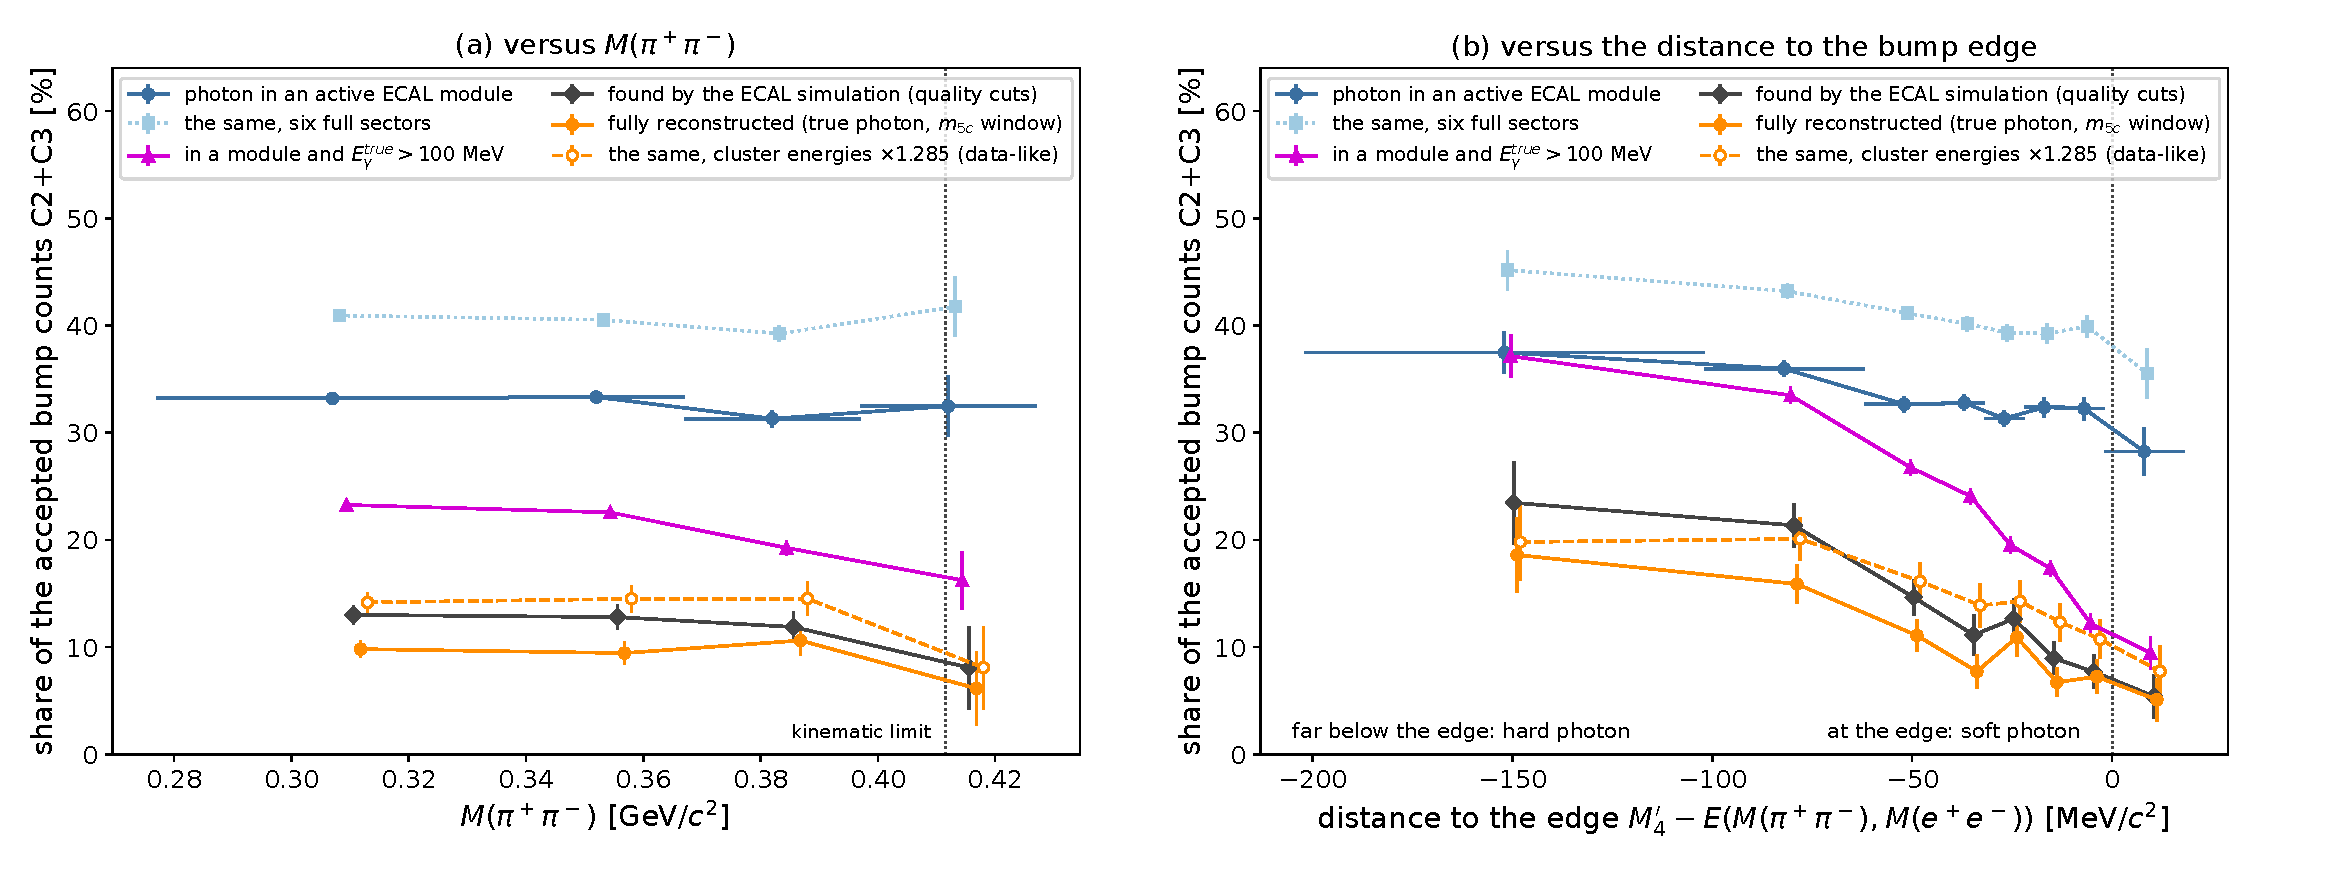
\includegraphics[width=0.96\textwidth]{figs_all/ecalacc_fractions_cnt.pdf}
\caption{\textbf{What it shows: one third of the lost bump photons hit an active ECAL module at every \Mpipi, but near
the edge the photon is too soft for the 100\,MeV threshold, so the full reconstruction sees preferentially the part of
the bump far below the edge.} Selection: SMASH simulation only (bump classes 2 and 3 come from the standard set; mode~A, PDG branching ratios $\times$ the $\eta$-decay physics weights V3); the accepted bump counts of classes 2 and 3 after the base selection ``pre'' (PT3 trigger (bit 8192 set), event vertex in the target region ($z>-160$\,mm), \betanew particle identification (pions within $3\sigma$, leptons within $5\sigma$ and with a RICH ring), corrected momenta of all four tracks, all stored combinations of each event (isBest\,$\ge0$)), all \Mfour and \Mee; (a) $\Mpipi\times0.9952$, (b) $M_4'=0.99615\,M_4$ (data scale of Part~III); ECAL quality cuts: identified as a photon (PID~1), $0.8<\beta<1.2$, $E_{\mathrm{cluster}}>100$\,MeV; fully reconstructed: the tag photon is the true one, $0.119\le M(\ee\gamma)<0.173$\,\GeVcc, $\Mee<0.10$\,\GeVcc, $m_{5c}$ in 0.49--0.62\,\GeVcc. Later finding of Part~III (file \code{figs_all/ecalacc_fractions_cnt.pdf} of
\code{report_all.pdf}); simulation only: accepted \ppee counts of the bump classes 2+3 (``C2+C3''), ``pre'', SMASH with the
physics weights V3, MC errors. Blue: photon in an active module; light blue: the same with six working sectors; magenta:
in a module and true energy above 100\,MeV; dark grey: found by the ECAL simulation with the quality cuts; orange: fully
reconstructed (tagged with the true photon, $m_{5c}$ in 0.49--0.62\,\GeVcc); open orange, dashed: the same with the
simulated cluster energies $\times1.285$ (the energy scale of the data). (a) Against \Mpipi (dotted: kinematic limit
0.4116\,\GeVcc). (b) Against the distance to the bump edge, $u=M_4'-E(\Mpipi,\Mee)$ (result~4).}
\label{fig:res_ecal}
\end{figure}

\textbf{11. Later finding (Part~III): the low-mass tail of the simulated $\eta$ peak.} \emph{In short:} the tail of the
simulated $\eta$ peak is made by the leptons, which lose momentum (bremsstrahlung) in the detector material; the generator
writes no radiative photon, so the radiation of the decay itself is missing; in the distance to the bump edge, $u$, the tail
reaches the edge. \emph{What was done:} Part~III (package peaktail, checked by an independent verifier with own code)
compared the reconstructed and the generated \Mfour of the simulated peak counts of class~4 ($\eta\to\pipi\gamma$, photon
converted) and class~5 ($\eta\to\ppee$) at $0.30\le\Mpipi<0.40$\,\GeVcc, and put the true momenta into the reconstructed
four-vectors to see which particles make the shift. \emph{What was found:} the generated four-body mass is a sharp line
(class~5: 547.998--548.002\,\MeVcc for 99.8\,\% of the counts; class~4 at most 1.5\,\MeVcc below it, because the conversion
pair, made by pair production, carries the whole photon four-momentum); the converter has no PHOTOS (its ``brems'' plugins
are nucleon-nucleon bremsstrahlung). About a quarter of the peak counts (class~4 26\,\%, class~5 24\,\%) have leptons whose
momentum loss lowers \Mfour by more than 5\,\MeVcc; in the counts lowered by more than 25\,\MeVcc the leptons make 38 of the
41\,\MeVcc (class~5) and 45 of 48\,\MeVcc (class~4), the pions about 2. The loss is one-sided (lepton $p/p_{\mathrm{true}}$
below 0.90 for 7.0\,\%, above 1.10 for 0.7\,\%); the counts without such a loss are symmetric. The tail shrinks with \Mpipi
(counts more than 15\,\MeVcc low: 15.5\,\% at 0.30--0.34, 3.3\,\% at 0.42--0.46\,\GeVcc), because the leptons get softer. In
$u$, 87\,\% of the peak lies in the step-fit range $-45\le u<+45$\,\MeVcc, 17\,\% below $u=+20$\,\MeVcc (73\,\% of these are
tail counts) and 5\,\% within 10\,\MeVcc of the edge. In the step fit the core and the tail of the peak term push the step in
opposite directions and cancel ($+162$ and $-158$ counts per unit of the peak scale): the size of the peak term hardly matters,
its shape does. The radiation of the decay itself (the \ee pair of the direct decay, leading-log estimate) would make the
class-5 tail 16--19\,\% larger (1.09--1.10 times for classes 4+5 together). \emph{What was expected:} a resolution tail on
both sides; the tail is one-sided and comes from the leptons. \emph{What it means:} the simulated tail is physical but
incomplete. Its size cannot be checked in the data (Part~III: $0.3\pm1.0$ times the simulated tail), and scaling it moves the
bump scale from the $u$ edge by $+6.8$\,\% per unit; Part~III keeps the simulated tail and takes half of it as a systematic
term, $t=1\pm0.5$ times the simulated tail (D40, approved by the analyst on 15 November 2026): $\pm3.4$\,\% on the bump scale
from the $u$ edge, $\pm8.8$\,\% on $\sigma$ from the peak side bands. A larger simulated $\eta\to\pipi\gamma$ sample (180
simulated entries in the fit region) and a simulation
with the radiation of the decay would settle it. \emph{Status:} later finding, simulation part (independently verified).
\emph{Evidence:} Fig.~\ref{fig:res_peaktail}. \emph{Details:} \S\ref{sec:s5acc} (resolution and scale), \S\ref{sec:s5blind}.

\begin{figure}[!htbp]
\centering
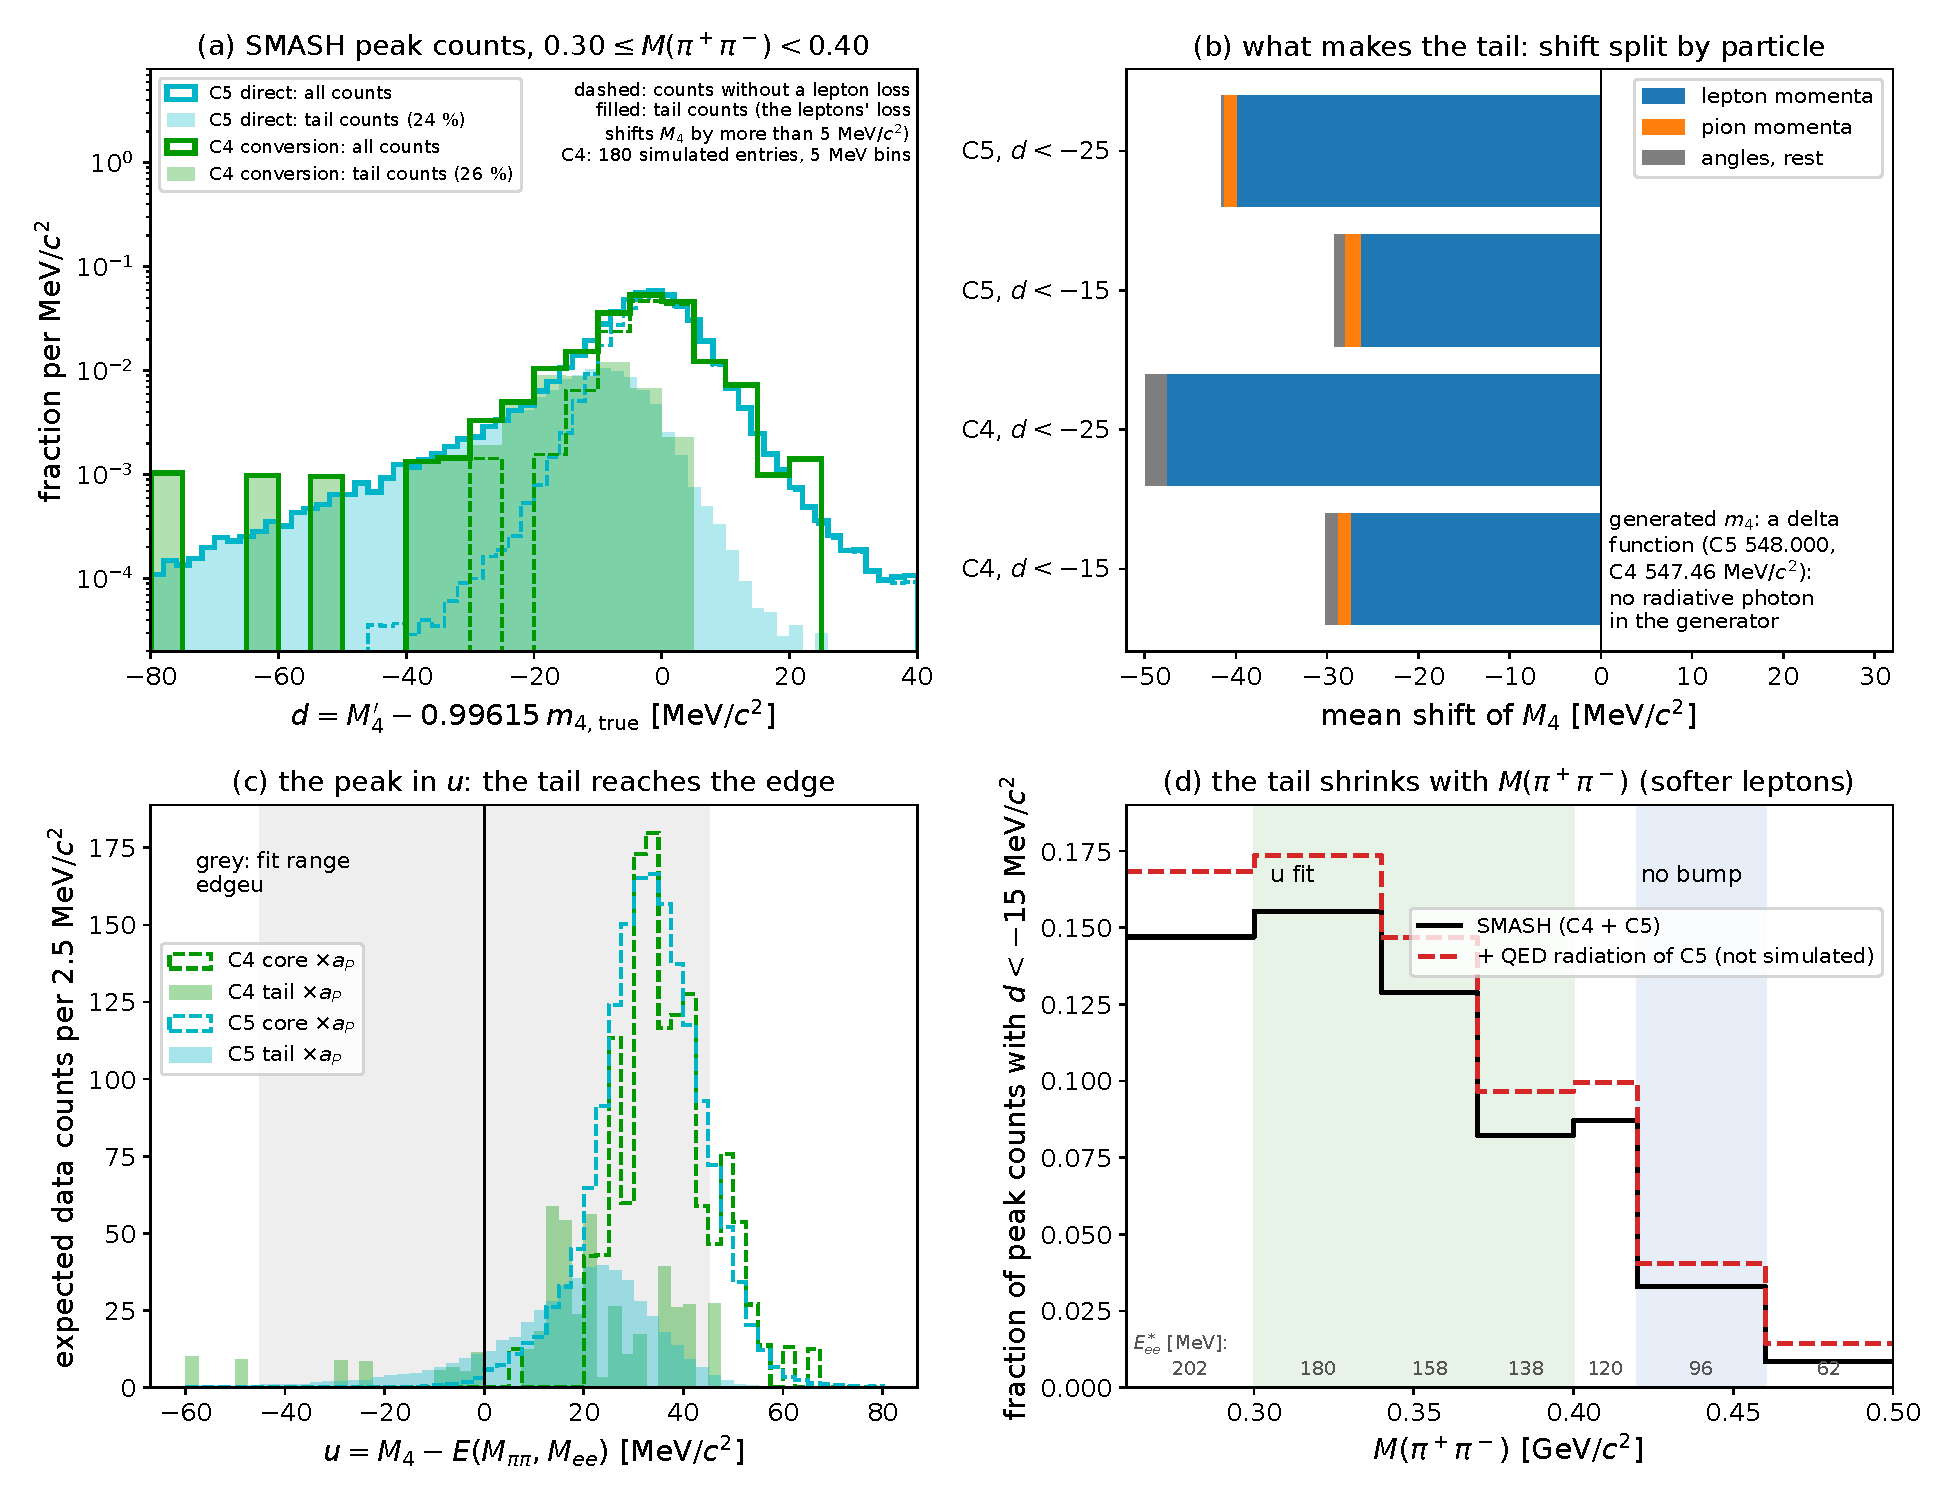
\includegraphics[width=0.90\textwidth]{figs_all/peaktail_sources_cnt.pdf}
\caption{\textbf{What it shows: the tail of the simulated $\eta$ peak comes from the leptons' momentum loss in the material,
not from the generator; in $u$ it reaches the bump edge, and it shrinks at large \Mpipi.} Selection: SMASH simulation only (mode~A, weights PDG branching ratios $\times$ V3, no combinatorial background); Part~III selection ``pre'' plus both pions used in the event-vertex fit (PT3 trigger (bit 8192 set), event vertex in the target region ($z>-160$\,mm), \betanew particle identification (pions within $3\sigma$, leptons within $5\sigma$ and with a RICH ring), corrected momenta of all four tracks, all stored combinations of each event (isBest\,$\ge0$)); the peak classes 4 ($\eta\to\pipi\gamma$, photon converted) and 5 ($\eta\to\ppee$) at all \Mee; masses on the data scale of Part~III, $M_4'=0.99615\,M_4$, $\Mpipi'=0.9952\,\Mpipi$; (a)--(c) $0.30\le\Mpipi'<0.40$\,\GeVcc, (c) in addition reconstructed $\Mee<135$\,\MeVcc, where $u$ is defined; (d) the \Mpipi' bins 0.26--0.30, 0.30--0.34, 0.34--0.37, 0.37--0.40, 0.40--0.42, 0.42--0.46 and 0.46--0.50\,\GeVcc; tail counts: the leptons' momentum loss lowers $M_4$ by more than 5\,\MeVcc. Later finding of Part~III (file
\code{figs_all/peaktail_sources_cnt.pdf} of \code{report_all.pdf}, package peaktail, checked by an independent verifier);
simulation only (SMASH, physics weights V3). (a) Residual $d=M_4'-0.99615\,m_{4,\mathrm{true}}$ of the simulated peak counts,
$0.30\le\Mpipi<0.40$\,\GeVcc: class~5 (cyan, 2\,\MeVcc bins) and class~4 (green, 180 simulated entries, 5\,\MeVcc bins); solid: all counts;
filled: tail counts (the leptons' momentum loss lowers \Mfour by more than 5\,\MeVcc; 24 and 26\,\%); dashed: the other counts,
symmetric. (b) Mean shift of \Mfour for counts with $d<-15$ and $<-25$\,\MeVcc, split into lepton momenta (blue), pion momenta
(orange) and angles and the rest (grey), from a linearised split (the verifier's substitution of the true momenta gives
2--3\,\MeVcc less for the leptons). (c) The peak in $u$ (expected data counts per 2.5\,\MeVcc, scaled by the peak scale 0.418
measured in Part~III): core counts dashed, tail counts filled; grey: the fit range of the $u$ step. (d) Share of peak counts with
$d<-15$\,\MeVcc per \Mpipi bin: SMASH (black) and SMASH plus the radiation of the direct decay that the generator lacks (red
dashed, leading-log toy); numbers: the \ee energy in the $\eta$ frame; shaded: the $u$-fit region and the region without bump.}
\label{fig:res_peaktail}
\end{figure}

\subsection{Summary of the headline numbers}
\label{sec:ressum}
Table~\ref{tab:summary} collects the headline numbers of Part~I, with the status of each and the place where it is
derived. Table~\ref{tab:summarylater} collects the later findings of Part~III that concern the simulation alone: the
bump edge in the distance $u$ (result~4), the ECAL and the lost photon of the bump (result~10), the class-2 QED factor
(result~7) and the low-mass tail of the $\eta$ peak (result~11).

\begin{table}[!tbp]
\centering
\caption{Headline numbers of Part~I (simulation only; rules~v2 with the physics weights V3 of the $\eta$ decays, which
are provisional). Counts in the data at $\Ldata = 6080.5\,\nbinv$ (not confirmed). Status: final = final for the
simulation with the provisional V3 weights; uncorr.\ = final, but not corrected for the later finding$^{a}$; prelim.\ =
preliminary; check = cross-check; frozen = fixed by the rule declared before the search; model = SMASH model value;
open = not resolved.}
\label{tab:summary}
\footnotesize
\setlength{\tabcolsep}{4pt}
\begin{tabularx}{\textwidth}{@{}L >{\raggedright\arraybackslash}p{6.3cm} >{\raggedright\arraybackslash}p{1.15cm} >{\raggedright\arraybackslash}p{1.55cm}@{}}
\toprule
Quantity & Value & Status & Details \\
\midrule
\multicolumn{4}{@{}l}{\textbf{Samples}} \\
luminosity of one simulated set, \Lsim & 221.05\,\nbinv ($10^{10}$ events) & final & Tab.~\ref{tab:norm} \\
data counts per unit of $\sum W$ & 27.51 & prelim. & Tab.~\ref{tab:norm} \\
$\eta$ production in SMASH, $\sigma_{\mathrm{prod}}(\eta)$ & $1.0665\pm0.0016$\,mb (200 files; 1.069\,mb from the generator count)$^{c}$ & model & Tab.~\ref{tab:smashprod}, \S\ref{sec:s5gen} \\
\midrule
\multicolumn{4}{@{}l}{\textbf{Signal channels after ``pre'', all \Mfour:} $\varepsilon$; $\sigma_{\mathrm{vis}}$; counts at \Ldata} \\
class 2, bump, $\eta\to\pipi\piz$, $\piz\to\ee\gamma$ & $0.245\pm0.007$\,\%; $7.05\pm0.19$\,nb; 42\,900 & uncorr.$^{a}$ & Tab.~\ref{tab:s5eps} \\
class 3, bump, a \piz photon converts & $0.00212\pm0.00007$\,\%; $5.19\pm0.17$\,nb; 31\,600 & final & Tab.~\ref{tab:s5eps} \\
class 4, peak, $\eta\to\pipi\gamma$, $\gamma$ converts & $0.00275\pm0.00017$\,\%; $1.24\pm0.08$\,nb; 7\,500 & final & Tab.~\ref{tab:s5eps} \\
class 5, peak, $\eta\to\ppee$ (direct) & $0.4944\pm0.0013$\,\%; $1.4168\pm0.0034$\,nb; 8\,600 & final & Tab.~\ref{tab:s5eps} \\
class 6, X17 at $\mathrm{BR}=10^{-5}$ & $0.6665\pm0.0010$\,\%; 0.0713\,nb; 430 & final & Tab.~\ref{tab:s5eps} \\
physical background (T2) & 686\,nb; 94\,\% of the sum T1+T2 (701.1\,nb) is multi-pion; fake leptons (T3) not included & final & \S\ref{sec:s5spec} \\
\midrule
\multicolumn{4}{@{}l}{\textbf{Closure and corrections}} \\
lepton/standard, \piz Dalitz pairs & $0.891\pm0.003$ (explained later$^{a}$) & check & \S\ref{sec:weights} \\
lepton/standard, $\eta$ Dalitz pairs & $0.879\pm0.005$ & check & \S\ref{sec:weights} \\
$\eta$ set/standard, counts without forced $\eta$ & $1.0056\pm0.0036$ & check & \S\ref{sec:weights} \\
peak share with $\Mee>20$\,\MeVcc & 0.219 with the weights (0.046 without; data$^{b}$ $0.280\pm0.071$; Part~II$^{d}$ $0.23\pm0.04\pm0.05$) & final & App.~\ref{sec:etagen} \\
peak kept by OA$>2^\circ$ & $0.697\pm0.015$ with the weights (0.59 without; data$^{b}$ $0.778\pm0.033$; Part~II$^{d}$ $0.772\pm0.037$) & open & App.~\ref{sec:etagen} \\
\midrule
\multicolumn{4}{@{}l}{\textbf{Cuts and frozen selections} ($F$ at \Ldata)} \\
purity in the window, ``pre'' $\to$ ``slides'' & bump $0.396\to0.371$; peak $0.198\to0.202$ & final & Tab.~\ref{tab:s5flow} \\
$F$, ``pre'' $\to$ ``slides'' & bump $152.7\to112.5$; peak $52.1\to41.0$ & final & Tab.~\ref{tab:s5flow} \\
PEAK frozen: $F$; gain over ``pre'' & $54.79\pm1.63$; $+2.67\pm0.44$ (5.1\,\%) & frozen & Tab.~\ref{tab:s5opt} \\
DIRECT frozen: $F$; gain over ``pre'' & $28.95\pm0.26$; $+1.12\pm0.10$ (4.0\,\%) & frozen & Tab.~\ref{tab:s5opt} \\
BUMP frozen & no cut (= ``pre''); $F = 152.7\pm3.0$ & frozen & Tab.~\ref{tab:s5opt} \\
optimisation bias of the freeze rule & below 1\,\% & check & \S\ref{sec:s5opt} \\
\midrule
\multicolumn{4}{@{}l}{\textbf{Extraction compared with the truth} (relative bias; coverage, nominal 0.683)$^{e}$} \\
peak: template fit M2 / Gaussian fit M1 & $+1.4$\,\% (0.77) / $+3.1$\,\% (0.72) & check & Tab.~\ref{tab:s5blind} \\
peak: linear side bands M3 & $-21.1$\,\% (0.53) in the PEAK toys; 13--46\,\% lost in all tests: not to be used & check & Tab.~\ref{tab:s5blind} \\
bump: side band B4 / edge step B3 & $+3.9$\,\% (0.66) / $+1.3$\,\% (0.76) & check & Tab.~\ref{tab:s5blind} \\
direct decay alone: M2d & $+20.6$\,\% (0.62) & check & Tab.~\ref{tab:s5blind} \\
common simulation error of a yield & peak $\pm$11--15\,\%, bump $\pm$4.5--5\,\% & final & \S\ref{sec:s5blind} \\
\midrule
\multicolumn{4}{@{}l}{\textbf{X17} (frozen selection v2; no X17 in the simulated sum)} \\
X17 counts at $\mathrm{BR}=10^{-5}$; background counts & 212.7; $5342\pm239$ & prelim. & Tab.~\ref{tab:s5x17} \\
expected 90\,\% CL limit & $1.9\times10^{-5}$ ($5.7\times10^{-6}$ with the background known exactly); later observed $3.16\times10^{-5}$$^{f}$ & prelim. & Tab.~\ref{tab:s5x17} \\
blind test: slope; median limits of the valid estimators & 0.98--1.02; 2.1--6.2$\times10^{-5}$ & check & \S\ref{sec:s5blind} \\
\bottomrule
\end{tabularx}

\raggedright{\footnotesize $^{a}$ Later finding (Part~III): HGeant decays the virtual photon of the \piz Dalitz decay
isotropically; the class-2 efficiency of the bump is about 16\,\% too high (Tab.~\ref{tab:summarylater}; toys, closure: 12--14\,\%); corrected in Part~III (D38).\\
$^{b}$ Measured outside Part~I: peak contents of the data study, quoted in the note
\code{docs/SYMULACJA_ETA_GENERATOR.md}.\\
$^{c}$ Later (Part~III): it uses $N_\eta=2.364\times10^8$, i.e.\ 1.0694\,mb; 1.0665\,mb is 0.28\,\% low.
$^{d}$ Later: final data values of Part~II (side bands; stat., method).\\
$^{e}$ Later finding (Part~III): with realistic template noise the template fits come out about 10\,\% low (cross-checks
only); main estimators: leak-corrected peak side bands and the bump edge step B3; B4 is not determined in the data
(result~4); also in $u$ (0.426, D37). $^{f}$ Later (Part~III): PDG 2026 (D25; PDG 2020: $3.06\times10^{-5}$);
expected $2.7\times10^{-5}$.}
\end{table}


\subsection{Key figures}
\label{sec:resfig}
Every result of \S\ref{sec:resmain} has its evidence figure in \S\ref{sec:resmain}: Fig.~\ref{fig:res_spec} shows what the
simulation predicts for the spectrum (result~1), Fig.~\ref{fig:res_cuts} what the usual $\eta$ cuts do inside the
windows (result~2), Fig.~\ref{fig:res_frozen} why the frozen selections were chosen (result~3), Fig.~\ref{fig:res_bias}
how well the planned extraction methods recover the true $\eta$ yields (result~4), Fig.~\ref{fig:res_x17} what sets
the expected X17 limit (result~5), Fig.~\ref{fig:res_gen} (left and middle) the corrected $\eta\to\ppee$ generator
(result~6), its right panel the decay angle behind the closure 0.891 (result~7) and Fig.~\ref{fig:res_pid} the PID cuts
(result~8). Result~9 (samples and normalisation) needs no figure: its numbers are luminosities and weights, given in
Tables~\ref{tab:sets}, \ref{tab:norm} and~\ref{tab:fat}. The same figures appear, with their full discussion, in
Sections~\ref{sec:pid} and~\ref{sec:simres}; the right panel of Fig.~\ref{fig:res_qed} is a panel of the Part~III summary
figure. Two later figures of Part~III are added because they change how results~4 and~5 are read:
Fig.~\ref{fig:res_stress} (its stress test of the extraction methods) and Fig.~\ref{fig:s5x17oa} (the opening angle of
the simulated X17); both also show data or data-based quantities, as their captions state. Result~10, a later finding of
Part~III from the simulation alone, has its evidence in Fig.~\ref{fig:res_ecal} (where the lost photon of the bump goes),
result~11 in Fig.~\ref{fig:res_peaktail} (where the tail of the $\eta$ peak comes from);
the kinematics of the bump edge in $u$ (result~4) are shown in Fig.~\ref{fig:res_edgeu}, and the ECAL coverage in
Fig.~\ref{fig:ecalgeo}.

\subsection{What is not determined, and why}
\label{sec:resnotdet}
\begin{itemize}\setlength{\itemsep}{1pt}
\item \textbf{The value of the cuts against the CB.} The simulation has no CB, so whether OA, $\alpha_{\mathrm{lab}}$,
      \Mpipi and $\alpha_\eta$ pay off in the data cannot be decided here (\S\ref{sec:s5spec}, \S\ref{sec:next}).
      \emph{Later (Parts~II, III):} decided in the data: they do not pay off (result~2).
\item \textbf{Collisions outside the liquid-hydrogen cell} (later, Parts~II and III). HGeant places the simulated vertices
      only in the target segments (card \code{JVER 2 2 0}; \code{start.geo} is commented out in its geometry), so the simulation
      has no collisions in the target walls or on the holder and no beam halo. Its vertex cut ($z>-500$\,mm) keeps 0.99970
      of the direct decays (171 of 572\,822 counts lost), all 307 counts of the conversion peak, 0.9994 and 0.9975 of the two
      bump classes and 0.991--0.996 of the K$^0_S$ pion pairs; $z>-160$\,mm then keeps 0.9975 of the direct decays. Only
      0.3\,\% of the simulated counts have at most one track in the window of the vertex finder (data: 35.6\,\%), the
      simulation always has a start-detector hit, and its track $z$ resolution at the vertex is better (rms 17.9 against
      23.7\,mm; the data beam axis is also off by (2.7, $-2.3$)\,mm). In the data 32\,\% of the \ee counts have no vertex;
      they are mostly not hydrogen events, probably from upstream of the cell (beam halo on the holder and the beam tube is the
      likely source, a hypothesis in Parts~II and~III), and hold no measurable $\eta$. The empty-target runs show that
      the target walls give 13--15\,\% of the data counts after CB subtraction in 0.40--0.70\,\GeVcc but only
      $3^{+4}_{-3}$\,\% of the $\eta$ (Part~III, its sections on the vertex efficiency and on the normalisation; its $\eta$
      yields are multiplied by $1-f_\eta$, approved by the analyst on 15 November 2026, D21).
\item \textbf{Fake leptons.} Counts with a misidentified or ghost track in a lepton slot (T3, 125.0\,nb against 701.1\,nb
      of T1+T2) are not in $B$, $F$ or the factor 46, but the data will contain them; with T3 and T4 added, $F$ of the
      peak at ``pre'' is 48.1 instead of 52.1 (Table~\ref{tab:s5flow}). \emph{Later (Part~III, D6 pending):} counting the
      ghost-flagged true pairs as physical background raises the simulation by 9--17\,\% (note after Table~\ref{tab:classes}).
\item \textbf{The absolute number of counts in the data.} It needs \Ldata (not confirmed), the SMASH production cross
      sections (model values, not compared with a measurement) and the data-side corrections (trigger, efficiencies);
      the counts quoted here are a scale (\S\ref{sec:xsec}). \emph{Later (Part~III, PRELIMINARY):} the data hold about
      0.4 of the SMASH $\eta$, $\sigma(pp\to\eta X)=0.43\pm0.17\,(\mathrm{measurement})\,^{+0.08}_{-0.03}\,(\mathrm{model})$\,mb
      (result~1); the model term is the dependence on the SMASH $\eta$ kinematics used for the extrapolation (D29).
\item \textbf{The direct decay alone.} \Mfour cannot separate it from the conversion peak; the split is limited by the
      307 standard-set entries of the conversion class (\S\ref{sec:s5blind}).
\item \textbf{An X17 limit close to the statistical one.} With the simulated background the limit is 3.4--3.5 times
      the statistical limit; a larger standard production or a background from data side bands is needed
      (\S\ref{sec:s5x17}). \emph{Later (Part~III):} done with the background from the data side bands (result~5).
\item \textbf{The effect of the beam energy.} The analysis uses $T = 4530$\,MeV, SMASH 4500\,MeV; \Mfour, \Mee and
      \Mpipi are not affected, the missing mass $\mathrm{MM}_4$ is, by an amount not yet quantified (App.~\ref{sec:beamT}).
      \emph{Later:} small (App.~\ref{sec:beamT}).
\item \textbf{Inputs not verified.} Whether the 1000 generator files behind the absolute efficiencies are
      representative; the X17 kinematics (phase-space \Mpipi, isotropic decay), which are assumed; the pion-vertex
      variables and the MDC energy loss, which were not compared with data (\S\ref{sec:s5data}, \S\ref{sec:pid}; Part~II later
      found the pion-vertex cut as efficient in data as in the simulation). \emph{Later (Part~III):} an independent count in
      40 files gives $1.0690\pm0.0035$\,mb, in line with the 1.069\,mb of the 1000 files (a partial check).
\end{itemize}

\subsection{Open questions}
\label{sec:resopen}
\begin{enumerate}\setlength{\itemsep}{1pt}
\item Why does OA$>2^\circ$ keep less of the simulated peak than of the data peak ($0.697\pm0.015$ against
      $0.778\pm0.033$, the data value measured outside Part~I) after the physics weights? (App.~\ref{sec:etagen})
      \emph{Later:} Part~II gives $0.772\pm0.037$ ($1.9\sigma$ from the simulation); Part~III sees relatively fewer close
      pairs in the data than in SMASH and proposes a close-pair loss in the data as a cause to be tested (its D32; result~6).
      The analyst ruled on 15 November 2026 that it is tested in a separate analysis (efficiency of \ee pairs with OA
      0--$6^\circ$ from \piz, $\eta$, $\omega$ Dalitz decays with the ECAL photon, in data and simulation).
\item Does the isotropic $\gamma^*$ decay of HGeant also lie behind the $\eta$ Dalitz closure $0.879\pm0.005$? The later
      finding of Part~III concerns the \piz Dalitz decay only (\S\ref{sec:weights}).
\item Was the tenfold $\eta\to\ee\gamma$ of the HGeant card intended? To be confirmed by the producers
      (App.~\ref{sec:hgeanteta}).
\item What causes the charge asymmetry of the ring-less electrons at large polar angle and high momentum, and is their
      high MDC energy loss the relativistic rise or the double deposit of a close pair? (\S\ref{sec:pid})
\item Why does the simulated ECAL find a cluster for only about 65\,\% of the photons inside its active modules?
      (Later finding, Part~III, result~10; known part: about 4\,\% of the counts have a cluster from an $e^\pm$ of the
      converted photon instead; cluster--track matching, cluster splitting and module edges were not followed, because only
      the found photons carry a cluster truth.) (\S\ref{sec:s5acc})
\end{enumerate}

\subsection{Decisions awaiting the analyst's ruling}
\label{sec:resdec}
The most consequential choices left open in the text (Part~I has no separate table of decisions; the remaining open
points are listed at the end of \S\ref{sec:s5data}).
\begin{enumerate}\setlength{\itemsep}{1pt}
\item \textbf{Pion-vertex cut in data:} add the $z$ of the pion tracks to the compact data entries (for the frozen
      $\Delta z_\pi$ selections), or use ``pre + both pions in the vertex fit'' (\S\ref{sec:s5opt}); since done in Part~II.
\item \textbf{Simulation statistics:} request a larger standard-set production, or determine the X17 background from
      data side bands (\S\ref{sec:s5data}). Later: the X17 background from the data side bands is done in Part~III; Part~III
      is still limited by the simulation statistics (its template-statistics error is 1.6--3.6 times the statistical one), so
      a larger standard production is still requested, and a forced $\eta\to\pipi\piz$ production ($\piz\to\ee\gamma$ and
      $\gamma\gamma$) with the full ECAL simulation, at least 10 times the present 2\,836 simulated entries of classes 2+3 (Part~III, ECAL
      study, result~10).
\item \textbf{Beam energy of the simulation:} analyse it with $T = 4500$\,MeV, or quantify the effect of 4530\,MeV on the
      cuts that use the beam (App.~\ref{sec:beamT}). Later: Part~III recomputes the simulated $\mathrm{MM}_4$ at
      4500\,MeV; the effect is small (App.~\ref{sec:beamT}).
\item \textbf{Requests to the producers:} confirm the HGeant setting $\mathrm{BR}(\eta\to\ee\gamma) = 6.0$\,\% and
      regenerate the $\eta$ set with $\eta\to\ppee$ defined through a dilepton (App.~\ref{sec:hgeanteta},
      \ref{sec:etagen}). Later (Part~III): a simulated ECAL energy scale and resolution matched to the data after the new
      ECAL calibration (the simulated cluster energy is 7--9\,\% low, result~10).
\item \textbf{A stricter blind test:} cut definitions only, hidden per-toy signal scales, no repeated entries and a CB-like
      component (\S\ref{sec:s5data}). Later: Part~III ran about 160\,000 estimator chains with realistic template noise and
      a CB built from the data like-sign pairs (result~4, Fig.~\ref{fig:res_stress}).
\item \textbf{Electrons in the \pim slot:} whether to add a momentum-dependent MDC energy-loss cut, after checking the
      energy loss in data (\S\ref{sec:pid}).
\end{enumerate}

\subsection{Symbols used in this section}
\label{sec:ressym}
{\footnotesize
\setlength{\tabcolsep}{4pt}
\renewcommand{\arraystretch}{1.08}
\begin{longtable}{@{}>{\raggedright\arraybackslash}p{3.2cm} >{\raggedright\arraybackslash}p{\dimexpr\textwidth-3.2cm-2\tabcolsep\relax}@{}}
\toprule
SMASH, PLUTO, HGeant & event generator of the p+p collisions; decay generator used to force decays (lepton and $\eta$ sets); GEANT3-based simulation of the HADES detector, which also decays \piz and $\eta$ in the standard set \\
PAT; RICH, MDC & PostDST Analysis Tool: builds the combinations of tracks and identifies the particles; ring-imaging Cherenkov detector (electron identification); drift chambers (tracking, energy loss) \\
count & one stored combination \pip\pim$e^+e^-$ of reconstructed tracks (one ntuple entry); an event can give several counts \\
``pre'' & base selection: all combinations (isBest $\ge0$), vertex $z>-500$\,mm, PT3 trigger, target region $z>-160$\,mm, momenta corrected for energy loss \\
\Lsim, \Ldata & integrated luminosity of one simulated set; of the data (not confirmed) \\
$W$; rules v2; V3 & physical weight of a count ($\sum W/\Lsim$ is a cross section); weight rules with the exact HGeant branching ratios; main variant of the physics weights of the $\eta$ decays (provisional) \\
$\sigma_{\mathrm{prod}}$, BR, $\varepsilon$ & production cross section in SMASH; branching ratio (PDG); acceptance $\times$ efficiency: counts after ``pre'' per produced decay \\
$\sigma_{\mathrm{vis}}$ & visible cross section of counts after ``pre'', $\sigma_{\mathrm{prod}}\times\mathrm{BR}\times\varepsilon$; counts in the data $=\sigma_{\mathrm{vis}}\,\Ldata$ \\
classes 2--6 & 2 bump with a \piz Dalitz pair, 3 bump with a converted photon, 4 peak from $\eta\to\pipi\gamma$ with conversion, 5 direct decay $\eta\to\ppee$, 6 X17 \\
T1, T2, T3; multi-pion & templates: signal (classes 2--6); physical background, i.e.\ counts with a true \ee pair from one source and any pions; fake lepton (a misidentified or ghost track in a lepton slot), not added to the simulated sum. Multi-pion: the part of T2 with a \piz Dalitz, conversion or vector-meson pair not attributed to an $\eta$ \\
CB & combinatorial background of the data (absent in simulation) \\
$\gamma^*$, $\theta^*$ & virtual photon of a Dalitz decay ($\gamma^*\to\ee$); emission angle of the $e^+$ in the rest frame of the $\gamma^*$ \\
peak / bump window & $0.5333\le\Mfour<0.5587$ / $0.4576\le\Mfour<0.5255$\,\GeVcc \\
OA, $\alpha_{\mathrm{lab}}$, $\alpha_\eta$ & \ee opening angle (lab); angle between the \pipi and \ee momenta (lab); the same angle in the rest frame of a hypothetical $\eta$ \\
$\mathrm{MM}_4$, $\Delta z_\pi$ & missing mass of \ppee; largest distance in $z$ between a pion track and the event vertex \\
$S$, $B$, purity, $F$, $F_{\mathrm{best}}$, $Q$ & signal counts and other T1+T2 counts in a window at \Ldata ($B$ is T1+T2 only, without fake leptons); $S/(S+B)$; $S/\sqrt{S+B}$; the largest $F$ of the scan; $\varepsilon_S/\sqrt{\varepsilon_B}$, the factor by which a cut changes $S/\sqrt{B}$ \\
toy, bias, coverage & one pseudo-data set drawn from half of the simulated events (the other half gives the templates); mean (extracted $-$ true); fraction of toys within the quoted error \\
M1, M2, M3, M2d, B3, B4 & Gaussian + polynomial; template fit; linear side bands; template fit with the conversion constrained; edge step; side band with the simulated shape \\
Later; D$n$ & a finding of Part~II (data, \code{report_exp.pdf}) or Part~III (data + simulation, \code{report_all.pdf}) made after this part; a numbered decision of Part~III \\
template noise & the statistical fluctuation of the simulated templates (finite simulation statistics); it biases a fit that scales a noisy signal template towards zero \\
target walls, beam halo & the entrance and exit windows and the wall of the liquid-hydrogen cell; beam particles off the beam axis that hit material around the target \\
$E(m,q)$, $u$ & the bump edge: the largest \Mfour that $\eta\to\pipi\piz$, $\piz\to\ee\gamma$ can give with the photon lost, for $\Mpipi=m$ and $\Mee=q$ (exact, with the \Mee term); the distance to it, $u=\Mfour-E(\Mpipi,\Mee)$ (later, Part~III) \\
ECAL; ECAL sector~0 & electromagnetic calorimeter of HADES (6 sectors of 163 lead-glass modules); its sector at azimuth 63--117$^\circ$, switched off in the data and in the simulation \\
fully reconstructed; ECAL tag & a bump count whose lost photon is found in the ECAL, so that $\pipi\ee\gamma$ gives the $\eta$ ($m_{5c}$ in 0.49--0.62\,\GeVcc); the number of such counts (Part~II) \\
\bottomrule
\end{longtable}
}

\begin{table}[!htbp]
\centering
\caption{\textbf{What it shows: the later findings of Part~III that concern the simulation alone.} Part~III packages
``edgeu'', ``eestep'', ``ecalacc'' and ``peaktail'' and the C2 factor
reconciliation, each checked by an independent verifier; simulation only, SMASH with the physics weights V3, ``pre''
unless stated. Status: later = later finding, simulation part; open = not resolved; D$n$ = decision of Part~III (D37--D40
approved by the analyst on 15 November 2026).}
\label{tab:summarylater}
\footnotesize
\setlength{\tabcolsep}{4pt}
\begin{tabularx}{\textwidth}{@{}L >{\raggedright\arraybackslash}p{6.3cm} >{\raggedright\arraybackslash}p{1.15cm} >{\raggedright\arraybackslash}p{1.55cm}@{}}
\toprule
Quantity & Value & Status & Details \\
\midrule
\multicolumn{4}{@{}l}{\textbf{The bump edge in $u=\Mfour-E(\Mpipi,\Mee)$}} \\
simulated bump counts above their exact edge & none (largest excess $-0.48$ / $-0.51$\,\MeVcc, classes 2 / 3); without the \Mee term 3.8\,\% of class~2 & later & \S\ref{sec:s5blind} \\
$u$ resolution at the edge & 6.7\,\MeVcc (Gaussian core; 5.8--7.1 by fit method); almost all from \Mfour & later & Fig.~\ref{fig:s5edgeu} \\
step at $u=0$ in simulated backgrounds & none (other $\eta$ counts: $123\pm53$, 2.3$\sigma$, template noise) & later & \S\ref{sec:s5blind} \\
like-sign pairs from the two \piz photons ($\eta\to\pipi\piz$, standard set) & present in SMASH, mostly $e^-e^-$, at large \Mee (around 100\,\MeVcc), part of the $e^-e^-$ ones with a Compton or knock-on electron; their edge is the bump edge (proof and toys); used for the origin only, no rate compared with the data & later; D39 & \S\ref{sec:s5blind} \\
charge flip, per true \ee pair / per true $e^+$ & 0.04 / 0.01 / 0.008\,\% (standard / lepton / $\eta$ set); 1.7\,\% below 100\,MeV$/c$, $\le0.06$\,\% above 300\,MeV$/c$ & later; D39 & \S\ref{sec:s5blind} \\
\midrule
\multicolumn{4}{@{}l}{\textbf{The low-mass tail of the $\eta$ peak} (classes 4+5, $0.30\le\Mpipi<0.40$\,\GeVcc)} \\
generated four-body mass & sharp line (class~5: 547.998--548.002\,\MeVcc for 99.8\,\%); no radiative photon, no PHOTOS & later & Fig.~\ref{fig:res_peaktail} \\
tail counts (lepton loss lowers \Mfour by $>5$\,\MeVcc) & class~4 26\,\%, class~5 24\,\%; leptons make 38 of 41 (class~5) and 45 of 48\,\MeVcc (class~4) of the shift below $-25$\,\MeVcc & later & \S\ref{sec:s5acc} \\
the peak in $u$ & 87\,\% in $-45\le u<+45$\,\MeVcc; 17\,\% below $+20$ (73\,\% tail counts); 5\,\% within 10\,\MeVcc of the edge & later; D40 & Fig.~\ref{fig:res_peaktail} \\
radiation of the decay (not simulated) & class-5 tail $\times$1.16--1.19 (leading log); classes 4+5 $\times$1.09--1.10 & later; open & \S\ref{sec:s5acc} \\
\midrule
\multicolumn{4}{@{}l}{\textbf{The ECAL and the lost photon of the bump} (classes 2+3)} \\
ECAL coverage seen from the target centre & 10.9--45.6$^\circ$; ECAL sector~0 off, 8 dead modules; 807 active modules, 8.45\,\% of $4\pi$ & later & Tab.~\ref{tab:ecalgeo} \\
lost photon: below / in / above the ECAL band & 9.0 / 54.5 / 36.5\,\% (9.9\,\% backward) & later & Fig.~\ref{fig:ecalgeo} \\
lost photon in an active ECAL module & $32.7\pm0.4$\,\% (40.3\,\% with six sectors), flat in \Mpipi & later & \S\ref{sec:s5acc} \\
lost photon in a module and above 100\,MeV & 21.6\,\% (13\,\% near the edge); mean photon energy 130\,MeV & later & \S\ref{sec:s5acc} \\
ECAL cluster for a photon inside a module & about 65\,\% at every energy (not explained); cluster energy 7--9\,\% low & open & \S\ref{sec:s5acc} \\
fully reconstructed bump counts & $9.8\pm0.6$\,\% (14.1\,\% at the energy scale of the data) & later & Fig.~\ref{fig:res_ecal} \\
counts with an ECAL tag & bump 12.7\,\%, class~4 0.8\,\%, class~5 1.8\,\% & later & \S\ref{sec:s5acc} \\
\midrule
\multicolumn{4}{@{}l}{\textbf{The class-2 QED angle factor in the full simulation}} \\
factor for the edge fits; all \Mfour; tagged counts & 0.86 ($u$: $0.861\pm0.007$; per slice: $0.860\pm0.010$); 0.864; 0.876 (toys 0.88, closure 0.891) & later; D38 & \S\ref{sec:weights} \\
\bottomrule
\end{tabularx}
\end{table}

\bigskip
\phantomsection
\addcontentsline{toc}{part}{How the results were obtained}
\part*{How the results were obtained}

%======================================================================
\section{Scope}
\label{sec:scope}
%======================================================================
\inshort{Part~I describes the simulation on which the search for the $\eta$ in \ppee rests (samples, normalisation,
weights, technical pitfalls, selection) and tests the cuts and the signal extraction on simulation alone. The $\eta$ is
expected as a peak at $m_\eta$ and as a much larger bump below it.}

The analysis looks for the $\eta$ meson in the final state $\ppee$ of p+p collisions at
$T = 4.5$\,GeV. Two structures are expected in the invariant mass $\Mfour$:
\begin{itemize}
\item the \textbf{peak} at $m_\eta$ from the decay $\eta\to\ppee$, and from
      $\eta\to\pipi\gamma$ when the photon converts into an \ee pair in the detector;
\item the \textbf{bump} below $m_\eta$ from $\eta\to\pipi\piz$ followed by the Dalitz decay
      $\piz\to\ee\gamma$ (or by a photon conversion), when the photon is not detected.
\end{itemize}
The bump is much larger than the peak and has a known branching ratio, so it can serve as a
reference. The \ee pairs of the peak are also the place to search for a hypothetical X17
boson ($\eta\to\pipi X17$, $X17\to\ee$).

This first part documents the simulation used for the analysis: the samples, their
statistics and normalisation, the weights, several technical pitfalls met on the way, and a
short description of the selection. The data analysis and the comparisons follow in later
parts (Sect.~\ref{sec:next}).

%======================================================================
\section{Simulation samples}
\label{sec:samples}
%======================================================================
\inshort{three sets of the same $10^{10}$ SMASH collisions, each worth $\Lsim = 221.05\,\nbinv$; physical weights $W$
make them addable ($\sigma = \sum W/\Lsim$). With the physical decay kinematics the signal channels have visible cross
sections from 1.24\,nb (conversion peak) to 7.05\,nb (bump with a \piz Dalitz pair); the physical background is
46 times the signal with the physics weights of the $\eta$ decays (about forty times before them).}

\subsection{Event generator and the three sets}
All simulated events come from one SMASH run: p+p at $T = 4.5$\,GeV, SMASH-3.0, collider
mode, impact parameter sampled uniformly in the area in $[0, 1.2]$\,fm. Every sampled event
is kept, including the 4.3\,\% without any interaction. The converter (\code{convert-smash})
turns the SMASH output into HGeant input; it was run three times on the \emph{same}
$10^{10}$ events, with different treatment of some particles (Table~\ref{tab:sets}).
This was verified: the converted files of the three sets are identical event by event apart
from the forced particles, and the reconstructed entries of different sets contain the same
generator pions (Sect.~\ref{sec:rotation}). The three sets therefore describe the same
collisions; only the detector simulation (HGeant) is independent in each set.

\begin{table}[H]
\centering
\caption{The three SMASH simulation sets. ``Forced'' means that the converter (with PLUTO)
replaced the natural decay of every such particle by the listed channel and stored a weight
on its products. Weight 0 in the file means ``not weighted'' (natural probability).}
\label{tab:sets}
\begin{tabularx}{\textwidth}{@{}>{\raggedright\arraybackslash}p{1.9cm} >{\raggedright\arraybackslash}p{5.7cm} L >{\raggedright\arraybackslash}p{2.9cm}@{}}
\toprule
Set & Converter run & What is changed & Weight stored on the products \\
\midrule
standard (\code{std}) & 2026-05-18, \code{-u 0}, no PLUTO &
  nothing; \piz and $\eta$ decay in HGeant; SMASH resonance decays ($\rho,\omega,\phi$) are
  only flagged in the generator code & 0 for every particle \\
lepton (\code{lep}) & 2026-02-11, PLUTO,\newline \code{database_decays_leptons.dat} &
  every \piz, $\eta$, $\rho^0$, $\omega$, $\phi$ forced into a dilepton channel
  (Table~\ref{tab:forced}) & $w = n_{\mathrm{ch}}\times\mathrm{BR}$ on the forced-decay products \\
$\eta$ (\code{eta}) & 2026-06-03, PLUTO,\newline \code{database_decays_eta.dat} &
  every $\eta$ forced: 50\,\% $\eta\to\ppee$, 50\,\% $\eta\to X17\,\pipi$, $X17\to\ee$
  ($m_{X17}=17$\,\MeVcc) & $w = 2$ on the four products \\
\bottomrule
\end{tabularx}
\end{table}

\begin{table}[H]
\centering
\caption{Normalisation, common to the three sets.}
\label{tab:norm}
\begin{tabularx}{\textwidth}{@{}l L@{}}
\toprule
Events per set & $N = 10^{10}$ (100\,000 files $\times$ 100\,000 events) \\
Area per event & $\pi b_{\max}^2 / N = 45.239\,\mathrm{mb}/10^{10} = 4.5239\times10^{-3}$\,nb \\
Integrated luminosity per set & $\Lsim = N/(\pi b_{\max}^2) = 221.05\,\nbinv$ \\
SMASH cross sections (for orientation) & $\sigma_{\mathrm{tot}} = 43.29\pm0.03$\,mb,
   $\sigma_{\mathrm{el}} = 12.72\pm0.06$\,mb, $\sigma_{\mathrm{inel}} = 30.57\pm0.07$\,mb \\
Expected counts in data & $N_{\mathrm{data}} = (\Ldata/\Lsim)\,\sum W$ (sum over the counts);
   for $\Ldata = 6080.5\,\nbinv$: 27.51 per unit weight \\
\bottomrule
\end{tabularx}
\end{table}

Because $\sigma_{\mathrm{tot}} < \pi b_{\max}^2$, the range of $b$ covers every SMASH
collision. The luminosity of a set does not depend on the SMASH cross sections; the
particle yields per collision do.

\subsection{Detector simulation and PAT production}
The three sets went through HGeant and the HADES reconstruction (DST production feb22,
\code{gen4}). The DSTs were processed with PAT (PostDST Analysis Tool) into the three
hypothesis trees of this analysis. Table~\ref{tab:prod} lists the production.

\begin{table}[H]
\centering
\caption{PAT production of the simulation (all three sets with the same frozen binary).}
\label{tab:prod}
\begin{tabularx}{\textwidth}{@{}l L@{}}
\toprule
PAT branch, commit & \code{pp45_sim_pippimepem}, \code{e674942} (binary built 2026-11-11 20:42) \\
Software & Hydra 2.7.6, ROOT 6.36.02 (Debian 12) \\
PID cut file & \code{pp45_pid_cuts_sim_betanew_v6.root}: p, \pip, \pim at $3\sigma$,
   $e^\pm$ at $5\sigma$ (Sect.~\ref{sec:pid}) \\
Hypotheses written & \code{PipPimEpEm_ID}, \code{PipPimEpEp_ID}, \code{PipPimEmEm_ID}
   (level after the PID cut) \\
DST input & \code{/lustre/hades/dstsim/feb22/p4500p/}\allowbreak\code{gen4/smash/smash_<set>/root/}, 100\,000
   files per set, all processed, $10^{10}$ events per set \\
Merged files & \code{ppee_std_all.root} (0.30\,GB), \code{ppee_lep_all.root} (10.0\,GB),
   \code{ppee_eta_all.root} (4.0\,GB) \\
\bottomrule
\end{tabularx}
\end{table}

\begin{table}[H]
\centering
\caption{Entries (combinations) and events of the PAT hypothesis trees. ``Events'' counts the
events with at least one entry.}
\label{tab:patrows}
\begin{tabular}{@{}l rr rr rr@{}}
\toprule
 & \multicolumn{2}{c}{\code{PipPimEpEm_ID}} & \multicolumn{2}{c}{\code{PipPimEpEp_ID}} &
   \multicolumn{2}{c}{\code{PipPimEmEm_ID}} \\
Set & entries & events & entries & events & entries & events \\
\midrule
std & 238\,074 & 220\,532 & 1\,146 & 1\,066 & 4\,850 & 4\,455 \\
lep & 7\,622\,819 & 7\,035\,072 & 207\,380 & 197\,954 & 498\,807 & 469\,069 \\
eta & 3\,508\,574 & 2\,869\,528 & 14\,042 & 12\,391 & 54\,156 & 45\,879 \\
\bottomrule
\end{tabular}
\end{table}

\subsection{The ECAL in the simulation (later finding of Part~III)}
\label{sec:ecalsim}
\inshort{the electromagnetic calorimeter (ECAL) of the simulation has 6 sectors of 163 modules; ECAL sector~0 (azimuth
63--117$^\circ$) is switched off and 8 further modules are dead, exactly as in the data. Seen from the target centre the
modules span 10.9--45.6$^\circ$ in polar angle, and the 807 active modules cover 8.45\,\% of $4\pi$. One third of the lost
photons of the bump hit them (Fig.~\ref{fig:ecalgeo}).}
Part~I did not use the ECAL. Part~III (package ``ecalacc'' and its independent verification) read the ECAL geometry
(\code{EmcGeomPar}) and module status (\code{EmcCellStatusPar}) of the parameter file of the gen4 DST production of this
simulation (\code{allParam_feb22_sim_run_17000_gen4_10032026.root}, release \code{FEB22SIM_v4a}) to find out how much of
the bump the ECAL can see. The modules are lead-glass blocks with a front face of $92\times92$\,mm, a pitch of 94\,mm and a
depth of 420\,mm; their front faces are about 2.4\,m from the target. The digitizer skips modules with status~0, so they
are dead in the simulation (Table~\ref{tab:ecalgeo}). Part~III found the same status in the data parameters of all four
data-taking periods.

\begin{table}[H]
\centering
\caption{\textbf{What it shows: the ECAL of the simulation covers 10.9--45.6$^\circ$ seen from the target, in five of its
six sectors.} ECAL geometry and module status of the simulation (gen4 parameter file; later finding of Part~III). Polar angle
$\theta$ of the module corners seen from the target centre ($z\approx-124$\,mm: the simulated vertex is uniform in
$-148\ldots-99$\,mm); azimuth $\phi$ of the corners. The range 11.5--47.5$^\circ$ quoted first in Part~III's package is
seen from $z=0$, not from the target, and is not the coverage. Dead single modules (sector/module): 1/24, 1/195, 3/160,
3/237, 4/129, 4/157, 5/240, 5/244.}
\label{tab:ecalgeo}
\small
\begin{tabular}{@{}c c c c c@{}}
\toprule
ECAL sector & modules & active & $\theta$ from the target centre [deg] & $\phi$ [deg] \\
\midrule
0 & 163 & 0 (switched off) & 11.0--45.6 & 62.8--117.1 \\
1 & 163 & 161 & 11.4--45.3 & 123.3--177.0 \\
2 & 163 & 163 & 11.1--45.2 & 183.5--237.0 \\
3 & 163 & 161 & 11.2--45.2 & 242.9--296.4 \\
4 & 163 & 161 & 11.1--45.1 & 302.6--356.4 \\
5 & 163 & 161 & 10.9--45.1 & 2.6--56.7 \\
\midrule
all & 978 & 807 & \multicolumn{2}{l}{active: 8.45\,\% of $4\pi$ (six full sectors: 10.3\,\%)} \\
\bottomrule
\end{tabular}
\end{table}

At a given polar angle a working sector covers 45--53$^\circ$ of its 60$^\circ$ of azimuth (the corners span about
54$^\circ$). The verifier checked the geometry empirically: the simulated clusters of the standard set occupy exactly the
807 active modules (none in ECAL sector~0, none in a dead module), and the photons from the target that make a cluster point
to 11.75--44.3$^\circ$ (0.1--99.9\,\% quantiles). Where the lost photon of the bump goes is described in
\S\ref{sec:s5acc} (note ``Later finding: the lost photon of the bump''); Fig.~\ref{fig:ecalgeo} shows its polar angle
against the coverage.

\begin{figure}[H]
\centering
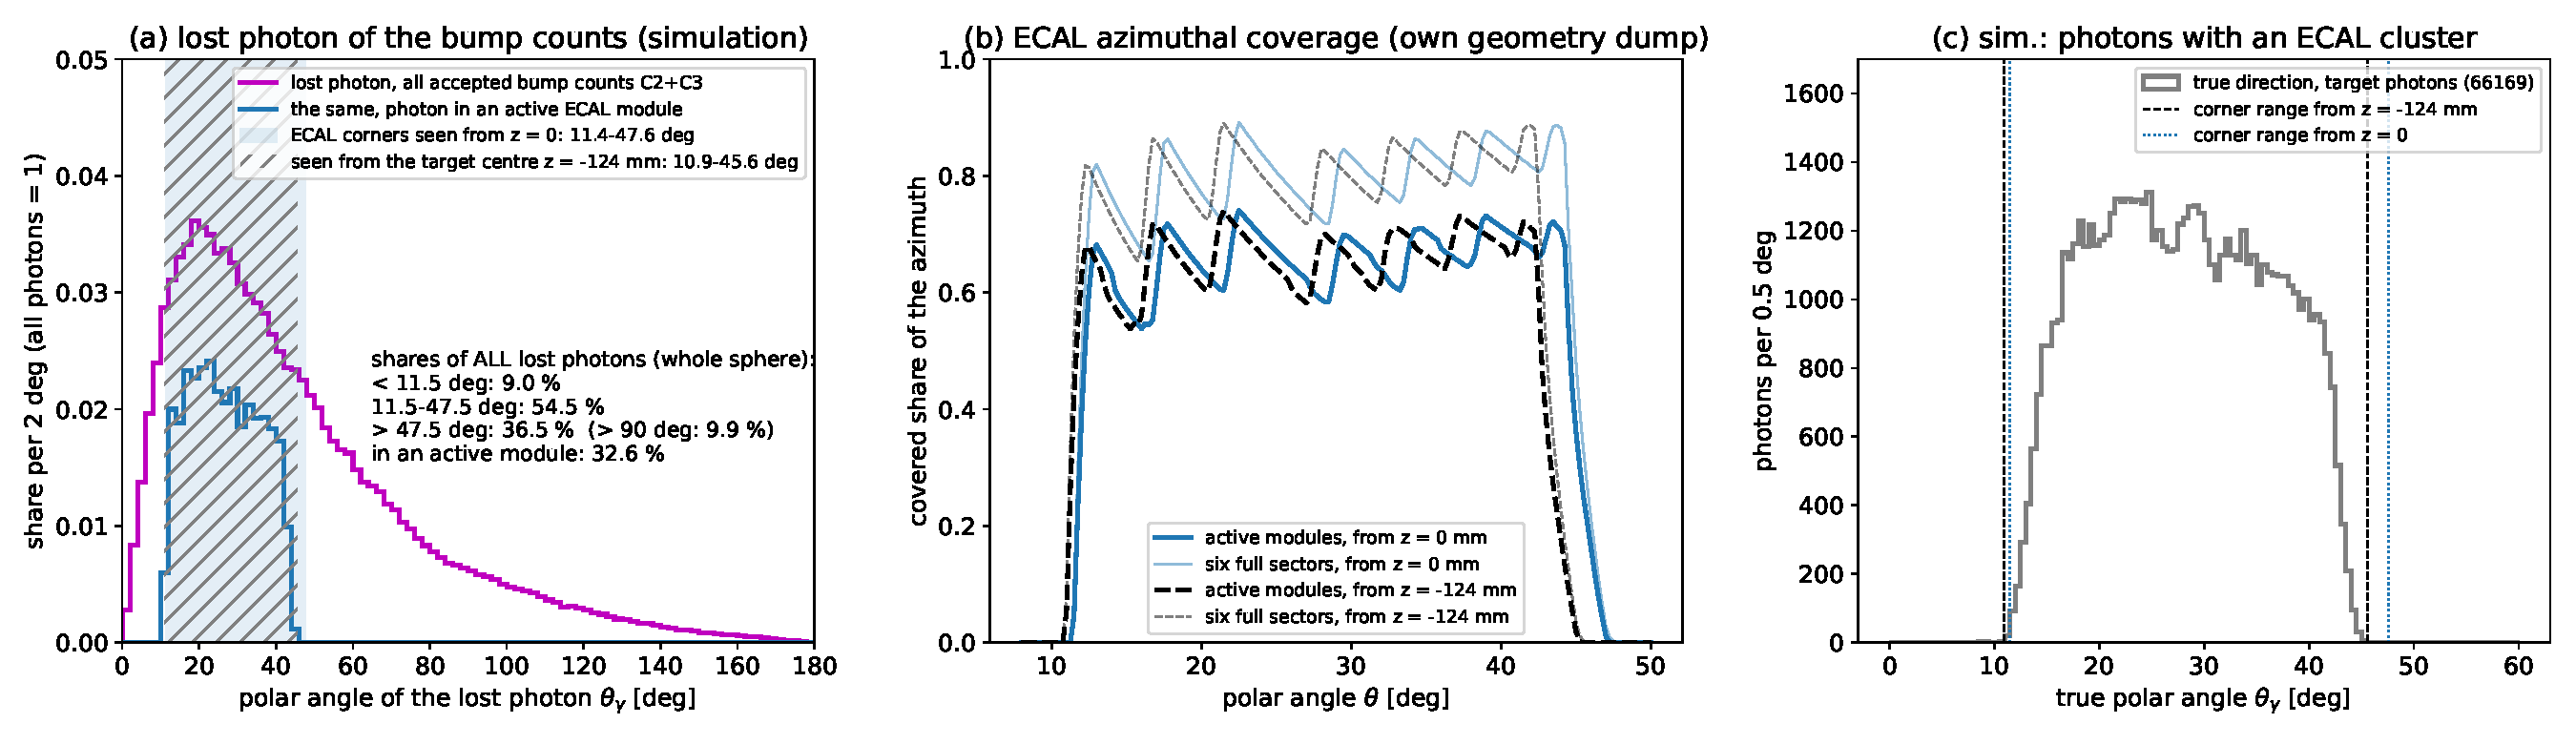
\includegraphics[width=\textwidth]{figs_all/vecalacc_theta_cnt.pdf}
\caption{\textbf{What it shows: one third of the lost bump photons hit an active ECAL module; over the whole sphere 9\,\%
fly below the ECAL, 55\,\% into its polar band and 37\,\% above it (10\,\% backward), and the ECAL seen from the real target
($z=-124$\,mm) covers 10.9--45.6$^\circ$.} Selection: (a) SMASH simulation only (mode~A, PDG branching ratios $\times$ V3): the accepted bump counts of classes 2 and 3 after the base selection ``pre'' (PT3 trigger (bit 8192 set), event vertex in the target region ($z>-160$\,mm), \betanew particle identification (pions within $3\sigma$, leptons within $5\sigma$ and with a RICH ring), corrected momenta of all four tracks, all stored combinations of each event (isBest\,$\ge0$)), at all \Mfour, \Mee and \Mpipi, with the verifier's own reconstruction of the lost photon on its circle; (b) geometry only, no counts; (c) every neutral candidate of every entry of the standard-set PAT file of the \ppee hypothesis, no further cut, whose true particle is a photon created near the target ($|z+124\,\mathrm{mm}|<40$\,mm, $r<10$\,mm). Later finding of Part~III (verification figure \code{figs_all/vecalacc_theta_cnt.pdf}
of \code{report_all.pdf}); simulation only. (a) Polar angle of the lost photon of the accepted bump counts (classes 2+3,
``pre''; the verifier's own reconstruction of the photon on its circle and its own SMASH sample), all (magenta) and those
in an active module (blue, 32.6\,\%; the package gives 32.7\,\%). Shaded: module corners seen from $z=0$; hatched: seen
from the target centre. (b) Covered share of the azimuth against the polar angle, for the active modules and for six full
sectors, seen from $z=0$ and from $z=-124$\,mm. (c) True polar angle of the target photons that made an ECAL cluster (all
standard-set events); dashed / dotted: the corner range seen from $z=-124$\,mm and from $z=0$.}
\label{fig:ecalgeo}
\end{figure}

\subsection{Analysis-framework processing and statistics}
The PAT trees are read by FAT (Final Analysis Tool, \code{main.cc}), which applies the
base selection of Sect.~\ref{sec:sel}, computes the kinematics and the truth classes, and
writes one entry per combination into the ntuple \code{scan_nt}. Table~\ref{tab:fat} gives the
statistics after each step.

\begin{table}[!htbp]
\centering
\caption{Statistics after the analysis framework. ``FAT entries'': $\mathrm{isBest}\ge0$,
vertex $z>-500$\,mm, PT3 trigger bit. ``Owned'': entries that this set provides in the
partition of Sect.~\ref{sec:weights} (mode A). $\sum W$: sum of the physical weights of the
owned entries with $z>-160$\,mm; $\sigma = \sum W/\Lsim$ is the visible cross section (Sect.~\ref{sec:xsec}) for producing such
a combination (pre-rw for the $\eta$ set). \emph{Later (Part~III):} the ratio FAT/PAT entries of the \ppee trees (0.968, 0.976,
0.959) is not the efficiency of the vertex cut, which is 0.9997 for the direct decay and 0.9989 for all weighted T1+T2 counts;
the drop comes mostly from the PT3 bit test (inferred, not measured separately). Earlier readings of these ratios as ``the
simulation keeps $\ge0.96$ after the vertex cut'' are superseded.}
\label{tab:fat}
\begin{tabular}{@{}l l r r r r r@{}}
\toprule
Set & Channel & PAT entries & FAT entries & $z>-160$ & owned & $\sigma$ [nb] \\
\midrule
std & \ppee        &   238\,074 &   230\,469 &   230\,115 &   115\,414 & 506.73 \\
    & $\pi^+\pi^-e^+e^+$ &  1\,146 &  1\,133 &  1\,132 &  1\,055 & 3.911 \\
    & $\pi^+\pi^-e^-e^-$ &  4\,850 &  4\,791 &  4\,777 &  4\,599 & 18.85 \\
\midrule
lep & \ppee        & 7\,622\,819 & 7\,441\,490 & 7\,432\,170 & 7\,082\,339 & 329.36 \\
    & $\pi^+\pi^-e^+e^+$ &   207\,380 &   205\,527 &   205\,288 &   159\,543 & 0.285 \\
    & $\pi^+\pi^-e^-e^-$ &   498\,807 &   495\,711 &   495\,101 &   328\,641 & 0.608 \\
\midrule
eta & \ppee        & 3\,508\,574 & 3\,366\,025 & 3\,357\,676 & 3\,180\,398 & 3.290 \\
    & $\pi^+\pi^-e^+e^+$ &    14\,042 &    13\,881 &    13\,856 &    13\,061 & 0.0134 \\
    & $\pi^+\pi^-e^-e^-$ &    54\,156 &    53\,628 &    53\,510 &    49\,892 & 0.0586 \\
\bottomrule
\end{tabular}
\end{table}

The large numbers of entries of the lepton and $\eta$ sets do not mean large cross sections: each
of their entries carries a small weight. For example, the 7.08 million owned \ppee entries of the
lepton set add up to $\sum W = 72\,804$, the 115\,414 entries of the standard set to
$112\,014$. The statistical power of a weighted sample is set by its effective number of
entries, $(\sum W)^2/\sum W^2$, not by the number of its entries.

\subsection{Weights}
\label{sec:weights}
Every count gets a physical weight $W$, so that $\sum W/\Lsim$ is a cross section and the
three sets can be added. The rules (version~2, \code{src/sim_truth.h}) are:
\begin{enumerate}
\item \textbf{Standard set.} $W=1$, with corrections of the HGeant branching ratios to PDG
      values for decays that HGeant performs (Table~\ref{tab:hgeant}). The largest correction
      is for $\eta\to\ee\gamma$: the HGeant configuration of this production sets its branching
      ratio to 8.8 times the PDG value (Sect.~\ref{sec:hgeanteta}), so an \ee pair from an $\eta$
      Dalitz decay gets the factor 0.114.
\item \textbf{Lepton set.} $W$ is the product of the weights of the \emph{distinct} forced
      decays found among the four tracks (Table~\ref{tab:forced}), with the PDG/database
      branching-ratio correction. A track from no forced decay contributes the factor 1.
      Two tracks belong to the same forced decay when their codes $(\code{geninfo},
      \code{geninfo2})$ agree (Sect.~\ref{sec:key}).
\item \textbf{$\eta$ set.} A count with the four products of one forced decay gets
      $W = 2\times\mathrm{BR}$: $\mathrm{BR}(\eta\to\ppee) = 2.68\times10^{-4}$ (PDG), and a
      hypothesis value for X17 (0 by default). Everything else in this set is the standard
      set without the natural $\eta$ decays.
\item \textbf{Ownership.} One type of count must come from one set only. In mode~A (default) the
      lepton set provides every count with a forced-decay product of a \piz, $\eta$, $\rho^0$,
      $\omega$ or $\phi$, and the standard set drops such counts; the $\eta$ set provides every
      count with a product of a forced $\eta$ decay. Mode~B (variant) leaves the \piz and $\eta$
      Dalitz counts in the standard set.
\end{enumerate}

\begin{table}[H]
\centering
\caption{Forced decays of the lepton set. The converter picks one of the $n_{\mathrm{ch}}$
active channels of a mother with equal probability, so the stored weight is
$n_{\mathrm{ch}}\times\mathrm{BR}$.}
\label{tab:forced}
\begin{tabular}{@{}l c l l l l@{}}
\toprule
Decay & $n_{\mathrm{ch}}$ & BR (database) & stored $w$ & BR (PDG) & PDG/database \\
\midrule
$\piz\to\ee\gamma$          & 1 & $1.198\times10^{-2}$ & 0.01198 & $1.174\times10^{-2}$ & 0.980 \\
$\eta\to\ee\gamma$          & 1 & $0.6\times10^{-2}$ & 0.006 & $0.69\times10^{-2}$ & 1.15 \\
$\rho^0\to\ee$              & 1 & $4.48\times10^{-5}$ & $4.5\times10^{-5}$ & $4.72\times10^{-5}$ & 1.054 \\
$\omega\to\ee$              & 2 & $7.15\times10^{-5}$ & $1.43\times10^{-4}$ & $7.38\times10^{-5}$ & 1.032 \\
$\omega\to\piz\ee$          & 2 & $5.9\times10^{-4}$ & $1.18\times10^{-3}$ & $7.7\times10^{-4}$ & 1.305 \\
$\phi\to\ee$                & 1 & $2.99\times10^{-4}$ & $2.99\times10^{-4}$ & $2.979\times10^{-4}$ & 0.996 \\
\bottomrule
\end{tabular}
\end{table}

\begin{table}[H]
\centering
\caption{Decays of \piz and $\eta$ performed by HGeant, and the correction factors applied to
counts with such decays (rules v2). ``Card'': the branching ratios in percent set in the HGeant
configuration of this production (\piz: HGeant default, no card); HGeant normalises them to
their sum. The producers' measurement on $10^6$ events (used in rules v1) agrees with the
normalised card within 0.3--2.2 standard deviations. The two \pipi modes of the $\eta$ cannot be
told apart for a pion; together they give the factor 1.047 (v1: 1.056).}
\label{tab:hgeant}
\small
\begin{tabular}{@{}l r l l l l l@{}}
\toprule
Mode & card [\%] & HGeant & measured & PDG & factor (v2) & (v1) \\
\midrule
$\piz\to\gamma\gamma$     & 98.798 & 0.98802 & $0.98798\pm0.00152$ & 0.98823 & 1.000 & 1.000 \\
$\piz\to\ee\gamma$        & 1.198 & 0.011980 & $0.01202\pm0.00017$ & 0.01174 & 0.980 & 0.977 \\
$\eta\to\gamma\gamma$     & 37.30 & 0.37555 & $0.3769\pm0.0040$ & 0.3936 & 1.048 & 1.044 \\
$\eta\to3\piz$            & 30.20 & 0.30406 & $0.3014\pm0.0036$ & 0.3257 & 1.071 & 1.081 \\
$\eta\to\pipi\piz$        & 21.00 & 0.21144 & $0.2074\pm0.0030$ & 0.2292 & 1.084 & 1.105 \\
$\eta\to\pipi\gamma$      & 4.75 & 0.047825 & $0.0497\pm0.0015$ & 0.0422 & 0.882 & 0.849 \\
$\eta\to\ee\gamma$        & \textbf{6.0} & \textbf{0.060410} & $0.0640\pm0.0016$ & \textbf{0.0069} & \textbf{0.114} & 0.108 \\
$\eta\to\gamma\gamma\piz$ & 0.071 & 0.000715 & -- & -- & -- & -- \\
$\eta\to\ppee$            & -- & absent & -- & 0.000268 & \multicolumn{2}{l}{from the $\eta$ set} \\
\bottomrule
\end{tabular}
\end{table}

The weight rules were checked by closure between sets: the same physics taken from two sets
must give the same weighted yield. For \piz Dalitz pairs the lepton/standard ratio is
$0.891\pm0.003$ (an unexplained offset of 0.954 times 0.934 from the different Dalitz
kinematics of PLUTO and HGeant); for $\eta$ Dalitz pairs it is $0.879\pm0.005$. Both Dalitz sources thus
show a similar deficit; the two values differ by 1.9 standard deviations. With the measured HGeant
branching ratio of rules~v1 the $\eta$ value was 0.931, 4\,\% above the \piz value. The counts of the $\eta$
set without a forced-$\eta$ track agree with the corresponding counts of the standard set to
$1.0056\pm0.0036$.

\notebox{\textbf{Later finding (Part~III).} The cause of the \piz Dalitz closure $0.891\pm0.003$ was found in
Part~III (\code{report_all.pdf}, section ``Efficiencies and the QED check of the bump simulation''): HGeant decays
the virtual photon of the \piz Dalitz decay ($\gamma^*\to\ee$) isotropically, while QED gives $1+\cos^2\theta^*$;
PLUTO, which decays the \piz of the lepton set, has the QED angle. The simulated efficiency of class~2 (bump with a
\piz Dalitz pair, standard set) is therefore too high: by 12--14\,\% for the prompt \piz Dalitz pairs of the closure, which
explains 0.891, and by about 16\,\% for the bump (next note). The numbers of this report are not corrected for it. Part~III
first applied a constant factor (0.8855, the mean of its toy and of this closure) to its bump-edge result only (D35; a toy
at the edge itself gives 0.883, and class~2 makes 54\,\% of the simulated step there), now per-count QED weights (D38).}

\notebox{\textbf{Later finding (Part~III, C2 factor reconciliation of 15 November).} The factor
$\varepsilon_{\mathrm{QED}}/\varepsilon_{\mathrm{iso}}$ of class~2 was then computed in the full simulation, count by count.
The lost photon of a bump combination is not stored, but the four true charged momenta, $m_{\piz}$ and $m_\eta$ fix it up to one
angle (a circle); the QED weight $3[1+c^2+e(1-c^2)]/(4+2e)$ ($c=\cos\theta^*$, $e=4m_e^2/\Mee^2$) was averaged along this
circle with the SMASH $\eta$ spectrum as density. Checks: a toy with the true photon reproduces the true mean to 0.0004;
in 359 simulated counts where the ECAL found the photon the exact weight is 0.866 against 0.867 from the circle.
Table~\ref{tab:c2recon} gives the factor: about 0.86 for the bump, not 0.88--0.89. It depends mainly on the momentum of
the softer lepton: 0.91 at 60--100\,\MeVc, 0.87 at 100--150\,\MeVc and 0.80--0.82 above 200\,\MeVc. The earlier toys
(0.875--0.883) cut sharply at 60\,\MeVc and so had too many soft leptons (34\,\% of the accepted decays below 80\,\MeVc
against 5\,\% in the full simulation); with a 100\,\MeVc cut the toy gives the full-simulation value. The closure 0.891
compares prompt \piz Dalitz pairs with another selection, and PLUTO and HGeant differ there in more than the angle (\Mee
spectrum 2\,\% harder); it stays the closure of prompt pairs. So the simulated class-2 efficiency of the bump is about
16\,\% too high, not 12--14\,\%. Part~III applied effectively 0.881 (D35), 2.4\,\% too high; since its D38 (approved by the
analyst on 15 November 2026, until a future simulation corrects the angle in GEANT itself, not expected) it applies these
per-count weights, and its bump scales rose by 1.4\,\% ($u$ edge, $0.420\to0.426$) and 1.2\,\% (per slice, $0.418\to0.423$).}

\begin{table}[!htbp]
\centering
\caption{\textbf{What it shows: the class-2 QED factor is about 0.86 for the bump in the full simulation; only a toy with
too many soft leptons gives 0.88.} Later finding of Part~III (C2 factor reconciliation): ratio of the class-2 efficiency
with the QED decay angle of the $\gamma^*$ to that with the isotropic angle of HGeant, class-2 counts of the standard set,
``pre'' + both pions in the vertex fit (Part~III's S0). For the two edge fits: the ratio of the simulated step fitted with
and without the weights. ``stat'': rms of 2000 replicas of the simulated event groups.}
\label{tab:c2recon}
\footnotesize
\begin{tabular}{@{}l c c c c@{}}
\toprule
class-2 counts & all \Mee & $\Mee<10$\,\MeVcc & $\Mee\ge10$\,\MeVcc & stat \\
\midrule
step of the fit in $u$ (distance to the edge) & 0.861 & 0.870 & 0.856 & 0.007 \\
step of the per-slice edge fit & 0.860 & 0.868 & 0.854 & 0.010 \\
counts with an ECAL tag & 0.876 & -- & -- & 0.009 \\
all \Mfour & 0.864 & 0.865 & 0.863 & 0.003 \\
bump window & 0.861 & 0.864 & 0.860 & 0.003 \\
$-15\ldots+5$\,\MeVcc from the edge & 0.855 & 0.858 & 0.853 & 0.005 \\
more than 60\,\MeVcc below the edge & 0.872 & 0.855 & 0.882 & 0.006 \\
toy, lepton momenta $>60$\,\MeVc & 0.884 & & & \\
toy, lepton momenta $>100$\,\MeVc & 0.862 & & & \\
\bottomrule
\end{tabular}
\end{table}

\subsection{Cross sections of the components}
\label{sec:xsec}
\textbf{What the cross sections in this report are.} Every $\sigma$ in Tables~\ref{tab:fat},
\ref{tab:tmpl} and~\ref{tab:cls} is a \emph{visible} cross section,
$\sigma_{\mathrm{vis}} = \sum W/\Lsim$: the cross section for producing a \emph{count} (a stored combination
of four tracks) that is reconstructed, passes the PID cuts and the base selection with
$z>-160$\,mm. It is the product of three factors of different origin:
\begin{enumerate}
\item the \textbf{production cross section} of the mother particle in p+p at 4.5\,GeV, taken from
      the \textbf{SMASH model} (Table~\ref{tab:smashprod}); it is not a measurement and has not yet
      been compared with one;
\item the \textbf{branching ratios} of the decays, \textbf{PDG} values (RPP 2020--2024 as quoted in the
      producers' note), imposed through the weights (Sect.~\ref{sec:weights},
      Tables~\ref{tab:forced} and~\ref{tab:hgeant}); for X17 a hypothesis. \emph{Later (Part~III, checked in the
      listings):} the weights use the PDG 2020 values ($\eta\to\pipi\piz$ 22.92\,\%, $\eta\to\pipi\gamma$ 4.22\,\%,
      $\eta\to\ppee$ $2.68\times10^{-4}$, $\piz\to\ee\gamma$ 1.174\,\%); PDG 2022 and 2024 already had 23.02\,\% and 4.28\,\%,
      and PDG 2026 gives $23.02\pm0.25$\,\%, $4.28\pm0.07$\,\%, $(2.76\pm0.16)\times10^{-4}$ ($S=1.5$) and an unchanged
      1.174\,\%. With PDG 2026 the visible cross sections of classes 2 and 3 would be $\times1.0044$, class~4 $\times1.0142$
      and class~5 $\times1.0299$; the numbers of this report are kept with PDG 2020;
\item the \textbf{acceptance times efficiency} (counts per decay), from the \textbf{HADES simulation}:
      HGeant, DST reconstruction, PAT (PID cuts, ranking) and the FAT base selection.
\end{enumerate}
Combinations are counted, not events: one count is one stored combination. The expected number of counts in data is $\sigma_{\mathrm{vis}}\,\Ldata$,
before the data-side corrections (trigger, efficiencies). Table~\ref{tab:cls} shows the three
factors separately for the signal classes; the templates of Table~\ref{tab:tmpl} sum over many
sources and are given only as totals.

\begin{table}[H]
\centering
\caption{Meson production in SMASH (p+p, $T = 4.5$\,GeV): mean number per collision
$\langle n\rangle$ and $\sigma_{\mathrm{prod}} = \langle n\rangle\,\pi b_{\max}^2 =
\langle n\rangle \times 45.239$\,mb. Counted in 200 of the 100\,000 converted input files
($2\times10^{7}$ events, every 500th file), the same files in all sets: $\eta$ and \piz directly in
the standard set (both are decayed later by HGeant); $\rho^0$, $\omega$, $\phi$ (decayed by SMASH)
as the forced dilepton decays of the lepton set, which replaces every such meson. Statistical
errors. These are model values, not measurements.}
\label{tab:smashprod}
\begin{tabularx}{\textwidth}{@{}L l r r@{}}
\toprule
Particle & counted in & $\langle n\rangle$ per collision & $\sigma_{\mathrm{prod}}$ [mb] \\
\midrule
\piz, all produced by SMASH (without the \piz of $\eta$ decays) & std & 0.42584 & $19.265\pm0.007$ \\
\quad of them not from $\omega$ or $\phi$ decays & lep & 0.41694 & $18.862\pm0.007$ \\
$\eta$ & std & 0.023574 & $1.0665\pm0.0016$ \\
$\rho^0$ & lep & 0.0096985 & $0.4388\pm0.0010$ \\
$\omega$ & lep & 0.0089169 & $0.4034\pm0.0010$ \\
$\phi$ & lep & 0.00022265 & $0.01007\pm0.00015$ \\
\bottomrule
\end{tabularx}
\end{table}

Cross-checks of the counts: the 471\,482 $\eta$ of the standard set equal the forced $\eta$ decays of
the $\eta$ set in the same files ($235\,656$ $\eta\to\ppee$ + $235\,826$ $\eta\to\pipi X17$, a split
of 49.98\,\%/50.02\,\%); the lepton set has 55 forced $\eta$ fewer, the $\eta$ of $\phi\to\eta\gamma$
(the $\phi$ is forced there). The \piz of the standard set equal those of the lepton set plus the
\piz of $\omega$ (177\,357) and $\phi$ (622) decays, within 3.

\emph{Later (Part~III):} for the whole simulated sample Part~III uses the $\eta$ count of \S\ref{sec:s5gen},
$N_\eta=2.364\times10^{8}$ in the $10^{10}$ events, i.e.\ 1.0694\,mb (an independent count in 40 files gives
$1.0690\pm0.0035$\,mb). The 1.0665\,mb of Table~\ref{tab:smashprod} is 0.28\,\% lower. Table~\ref{tab:cls} builds
$N_{\mathrm{gen}}$ of classes 2--4 from 1.0665\,mb, so their $\varepsilon$ are 0.28\,\% too high; $\sigma_{\mathrm{vis}}$ does not
change (it does not use $N_{\mathrm{gen}}$).

\textbf{Truth classes and templates.} Every simulated count (a \ppee combination) is classified
from the GEANT truth of its four tracks and the generator codes (\code{src/sim_truth.h}): the
lepton pair gets a class L0--L11, the pion pair a class P0--P9, the four particles together a
class 0--8, and the count a template T1--T4 (Table~\ref{tab:classes}). The templates are the
coarse split used everywhere: the simulated spectrum is T1+T2, while T3 and T4 are shown only
separately. Section~\ref{sec:simres} splits T2 further into groups $G$ (Table~\ref{tab:s5defs}).

\begin{table}[!htbp]
\centering
\caption{Truth classes of a simulated count (columns \code{sim_lcls}, \code{sim_pcls}, \code{sim_cls},
\code{sim_tmpl} of \code{scan_nt}). ``Same'' means one decay of one mother particle; ``FD'' a product of a
decay forced by the converter. Ghost: a reconstructed track flagged \code{sim_isghost}.}
\label{tab:classes}
\footnotesize
\begin{tabularx}{\textwidth}{@{}l L@{}}
\toprule
\multicolumn{2}{@{}l}{\textbf{Lepton pair} (\code{sim_lcls})} \\
L0 & a track in a lepton slot is not the expected lepton (misidentified) \\
L1 / L2 & both leptons from the same \piz / $\eta$ Dalitz decay \\
L3 & both leptons from the same photon conversion \\
L4 / L5 / L6 & $\rho^0,\omega,\phi\to\ee$ / $\omega\to\piz\ee$ / Dalitz decay of the \piz of $\omega\to\piz\ee$ \\
L7 / L8 / L9 & leptons from two different Dalitz decays / a Dalitz decay and a conversion / other different sources \\
L10 / L11 & ($\eta$ set) leptons of a forced $\eta\to\ppee$ / of the X17 \\
\midrule
\multicolumn{2}{@{}l}{\textbf{Pion pair} (\code{sim_pcls})} \\
P0 / P1 & a track in a pion slot is not a pion / a pion that decayed into a muon \\
P2 / P3 / P4 / P5 / P6 & both pions from the same $\eta$ / $\omega$ / $\rho^0$ / $\phi$ / $K^0_S$ \\
P7 & both pions primary (SMASH final state, different or no resonance) \\
P8 / P9 & mixed or secondary / ($\eta$ set) the pions of a forced $\eta\to\ppee$ \\
\midrule
\multicolumn{2}{@{}l}{\textbf{Four particles} (\code{sim_cls})} \\
0 / 1 & a misidentified particle / a pion decayed into a muon \\
2 / 3 & bump: $\eta\to\pipi\piz$, $\piz\to\ee\gamma$ / the same with a converted \piz photon \\
4 / 5 / 6 & peak: $\eta\to\pipi\gamma$ with conversion / $\eta\to\ppee$ / $\eta\to\pipi X17$ \\
7 / 8 & pions with an \ee pair from one source / leptons from different sources \\
\midrule
\multicolumn{2}{@{}l}{\textbf{Template} (\code{sim_tmpl})} \\
T1 signal & classes 2--6 (also with a ghost lepton track) \\
T2 physical background & a true \ee pair from one source (L1--L6; in the $\eta$ set also L10, L11 outside the
   signal) with any pions, no fake lepton \\
T3 fake lepton & L0, a ghost track in a lepton slot, or the same particle in both lepton slots \\
T4 different sources & L7--L9: neither signal nor background of one source (in data part of the
   combinatorial background) \\
\bottomrule
\end{tabularx}
\end{table}

\emph{Later (Part~III, its decision D6, ruling pending):} the ghost flag is treated asymmetrically here. A signal count with a
ghost lepton track stays in T1, while a true \ee pair of the background with a ghost track goes to T3 and is not in the
simulated sum. Part~III's variant (a) moves the ghost-flagged true pairs from T3 into T2: it raises the simulated T1+T2 by
9--17\,\% per \Mfour region (``pre'' + both pions in the vertex fit, all \Mfour: 616.5 $\to$ 716.1\,nb) and lowers the
data/simulation ratios by 8.5--14.5\,\%.

\begin{table}[!htbp]
\centering
\caption{Templates of the owned \ppee entries ($z>-160$\,mm), visible cross sections (see the text
above). Signal: the four tracks come exactly from one of the signal channels
(Table~\ref{tab:cls}). Physical background: a true \ee pair from one source with any pions. Fake
lepton: a misidentified track or a ghost track in a lepton slot, or the same particle in both
lepton slots. Different sources: the two leptons come from different decays.}
\label{tab:tmpl}
\begin{tabular}{@{}l rr rr rr@{}}
\toprule
 & \multicolumn{2}{c}{std} & \multicolumn{2}{c}{lep} & \multicolumn{2}{c}{eta (pre-rw)} \\
Template & entries & $\sigma$ [nb] & entries & $\sigma$ [nb] & entries & $\sigma$ [nb] \\
\midrule
T1 signal              &  3\,143 & 14.97 &           0 & --     & 1\,358\,905 & 1.385 \\
T2 physical background & 86\,834 & 380.00 & 6\,154\,438 & 303.89 &  1\,622\,996 & 1.518 \\
T3 fake lepton         & 22\,370 & 99.81 &    536\,261 & 24.95 &    165\,069 & 0.351 \\
T4 different sources   &  3\,067 & 11.96 &    391\,640 & 0.519 &     33\,428 & 0.036 \\
\bottomrule
\end{tabular}
\end{table}

\begin{table}[!htbp]
\centering
\caption{Signal classes ($z>-160$\,mm, all $\Mfour$): from production to observed counts,
$\sigma_{\mathrm{vis}} = \sigma_{\mathrm{prod}}(\eta)\times\mathrm{BR}\times\varepsilon$.
$\sigma_{\mathrm{prod}}(\eta) = 1.0665$\,mb (SMASH, Table~\ref{tab:smashprod}).
BR: PDG; X17 a hypothesis, $10^{-5}$ for illustration.
$N_{\mathrm{gen}}$: decays generated in the $10^{10}$ events; classes 2--4 in the standard set,
$N_\eta\times\mathrm{BR}_{\mathrm{HGeant}}$ with the HGeant values of Table~\ref{tab:hgeant}; classes 5, 6:
the forced decays of the $\eta$ set (counted, Table~\ref{tab:smashprod}).
$\varepsilon$ = counts$/N_{\mathrm{gen}}$: acceptance times efficiency, for classes 3 and 4 including the
probability that the photon converts; it does not depend on any weight. $\sigma_{\mathrm{vis}}$ (rules
v2): with the decay kinematics of the generators (HGeant phase space, PLUTO for class 5) and with
the physical decay kinematics (physics weights, Sect.~\ref{sec:etagen}; $\varepsilon$ changes by
0.889, 0.892, 1.014, 1.023). Errors: statistical, from the number of counts (and 0.15\,\% from
$\sigma_{\mathrm{prod}}$). Class 5: the weights assume that exactly half of the $\eta$ are forced into
\ppee; the count gives 49.98\,\%, so the product of the factors is 1.386 instead of the 1.385\,nb of the
weighted counts. Rules v1 gave 8.05, 5.93, 1.18 and 1.385\,nb in the generator column.}
\label{tab:cls}
\footnotesize
\setlength{\tabcolsep}{3.5pt}
\begin{tabular}{@{}c >{\raggedright\arraybackslash}p{3.0cm} >{\raggedright\arraybackslash}p{1.55cm} r r r l r r@{}}
\toprule
 & & & $\sigma_{\mathrm{prod}}\times\mathrm{BR}$ & & & & \multicolumn{2}{c}{$\sigma_{\mathrm{vis}}$ [nb]} \\
Class & Process & BR (PDG) & [nb] & $N_{\mathrm{gen}}$ & counts & $\varepsilon$ & generator & physical \\
\midrule
2 & $\eta\to\pipi\piz$, $\piz\to\ee\gamma$ & $0.2292\times$ $0.01174$ & 2\,870 & $5.97\times10^{5}$ & 1\,649 & $2.76\times10^{-3}$ & $7.92\pm0.20$ & 7.05 \\
3 & $\eta\to\pipi\piz$, $\piz\to\gamma\gamma$, one $\gamma\to\ee$ & $0.2292\times$ $0.98823$ & 241\,560 & $4.92\times10^{7}$ & 1\,187 & $2.41\times10^{-5}$ & $5.82\pm0.17$ & 5.19 \\
4 & $\eta\to\pipi\gamma$, $\gamma\to\ee$ & 0.0422 & 45\,005 & $1.13\times10^{7}$ & 307 & $2.72\times10^{-5}$ & $1.23\pm0.07$ & 1.24 \\
5 & $\eta\to\ppee$ & $2.68\times10^{-4}$ & 285.8 & $1.18\times10^{8}$ & 571\,246 & $4.85\times10^{-3}$ & $1.385\pm0.003$ & 1.417 \\
6 & $\eta\to\pipi X17$, $X17\to\ee$ & $10^{-5}$ (hyp.) & 10.66 & $1.18\times10^{8}$ & 787\,659 & $6.68\times10^{-3}$ & 0.0712 & 0.0712 \\
\bottomrule
\end{tabular}
\end{table}

Three points matter for the use of these numbers:
\begin{itemize}
\item The standard set gives the bump and the conversion peak with only 1\,649, 1\,187 and
      307 simulated entries: their statistical errors (2.5--6\,\%) will limit template fits.
\item Conversions are a large part of the simulated bump (42\,\%) and almost half of the
      simulated peak.
\item The physical background summed over the sets is 685\,nb, about forty times the signal
      (16.4\,nb, pre-rw).
      Most of it is multi-pion production with a \piz Dalitz or conversion pair, which SMASH
      does not describe well above the $\eta$ mass. \emph{Later (Part~III):} without any adjustment the ratio
      data/SMASH is 0.86 in the bump window, 1.10 in the peak window, 1.27 just above the peak and 0.74 at
      0.90--1.10\,\GeVcc; one common scale leaves $\chi^2/\mathrm{ndf}=12$. Part of the excess above the peak is the
      target material, which the simulation does not contain (\S\ref{sec:resnotdet}).
\end{itemize}

\subsection{Luminosity for the normalisation to data}
\label{sec:lumi}
The simulation is normalised to the data with $\Ldata$. The value $6080.5\,\nbinv$ comes
from the producers' note and has not been confirmed by a luminosity analysis of this data
set; in this report it is a parameter, and simulated results are also given per \nbinv and
as shapes. A comparison in absolute units needs, in addition, the data-side corrections
(trigger, efficiencies) that the analysis applies anyway.

\emph{Later (Part~II, \code{report_exp.pdf}, section ``Luminosity''):} 6080.5\,\nbinv is the luminosity of the
START-free analysis of elastic p+p scattering for all 17\,615 runs, $6080.5\pm5.2\,(\mathrm{stat})\pm337.9\,(\text{HADES
syst.})\pm62.6\,(\sigma_{\mathrm{int}}\text{ fit})\pm243.2\,(\text{normalisation})\,\nbinv$ (6.9\,\% in total), for the
liquid hydrogen only. The runs present in the data give 6079.2\,\nbinv, which Parts~II and III use; the absolute value is
still provisional there.

%======================================================================
\section{The analysis in brief}
\label{sec:ana}
%======================================================================
\inshort{PAT builds every combination of tracks that fits a hypothesis and identifies the particles with $\betanew$;
the analysis keeps all combinations ($\mathrm{isBest}\ge0$). The simulation and experiment PID cuts differ little.
Electrons without a RICH ring make 2.5\,\% of the \pim slot after the PID cut; a cut on the MDC energy loss reduces
them to 0.4\,\%, not yet checked in data. PID efficiencies depend on the partner tracks and are taken from complete
combinations.}

\subsection{Hypotheses and combinations}
PAT builds, in each event, every combination of tracks that fits a hypothesis with the right
charges: \ppee (\code{PipPimEpEm_ID}) for the signal, and the like-sign \pipi$e^+e^+$ and
\pipi$e^-e^-$ for the combinatorial background in data, $\mathrm{CB} = 2\sqrt{N_{++}N_{--}}$
times a correction factor $k$ determined from data. A lepton slot takes only tracks with a correlated RICH ring
(\code{HParticleCand::getRingCorr()}); a pion slot takes the tracks without one. In
simulation PAT also drops tracks without a GEANT identity. All particles of a combination must pass the PID cut of their slot
(Sect.~\ref{sec:pid}). The combinations of an event are ranked by a $\chi^2$ of the times of
flight; the best has $\mathrm{isBest} = 1$, the others $\mathrm{isBest} = 0$. This analysis
keeps all combinations, $\mathrm{isBest}\ge0$.

In simulation no combinatorial background is subtracted. The signal of a channel is the set
of counts whose four tracks come, according to the GEANT truth and the generator codes, exactly
from that production and decay channel; this is the equivalent of the data signal after CB
subtraction. The like-sign trees of the simulation are used only for side studies
(combinatorics, \code{isBest}) and to identify, qualitatively, the origin and kinematics of a structure seen in the data
(later, Part~III: D39); their rates are never compared with the data, because the simulation does not model the like-sign
or combinatorial background.

\subsection{\texorpdfstring{Particle identification with $\beta_{\mathrm{new}}$}{Particle identification with beta\_new}}
\label{sec:pid}
The PID uses the plane $(p, \betanew)$: the momentum from tracking and a velocity
reconstructed without a start detector, from the relative times of flight of the tracks of
the hypothesis. The cuts are polygons around the bands of p, \pip, \pim, $e^+$ and $e^-$,
fitted at several widths ($1\sigma$ to $5\sigma$) on PID samples; the productions use $3\sigma$
for p and $\pi^\pm$ and $5\sigma$ for $e^\pm$. The experiment cuts (\code{betanew_v1}) were
fitted on data, the simulation cuts (\code{betanew_v6}) on the SMASH simulation with the
GEANT truth of all particles of the hypothesis. In both files the two lepton cuts are
identical (experiment: the $e^-$ cut is a copy of the $e^+$ cut; simulation: the $e^+$ cut is
a copy of the $e^-$ cut).

Figure~\ref{fig:banana} is the summary of the PID: simulated tracks before the PID cut,
each measured in a slot whose mass hypothesis is its own kind, with the cuts used in the
simulation (solid) and in the experiment (dashed). Protons and pions come from the hadron PID
sample (hypothesis p\pip\pim), electrons and positrons from the lepton PID sample (hypothesis
\ppee); neither sample has a trigger condition. Figure~\ref{fig:leptons} enlarges the lepton
region. The two sets of cuts differ little: the simulated bands are slightly narrower.

\begin{figure}[!htbp]
\centering
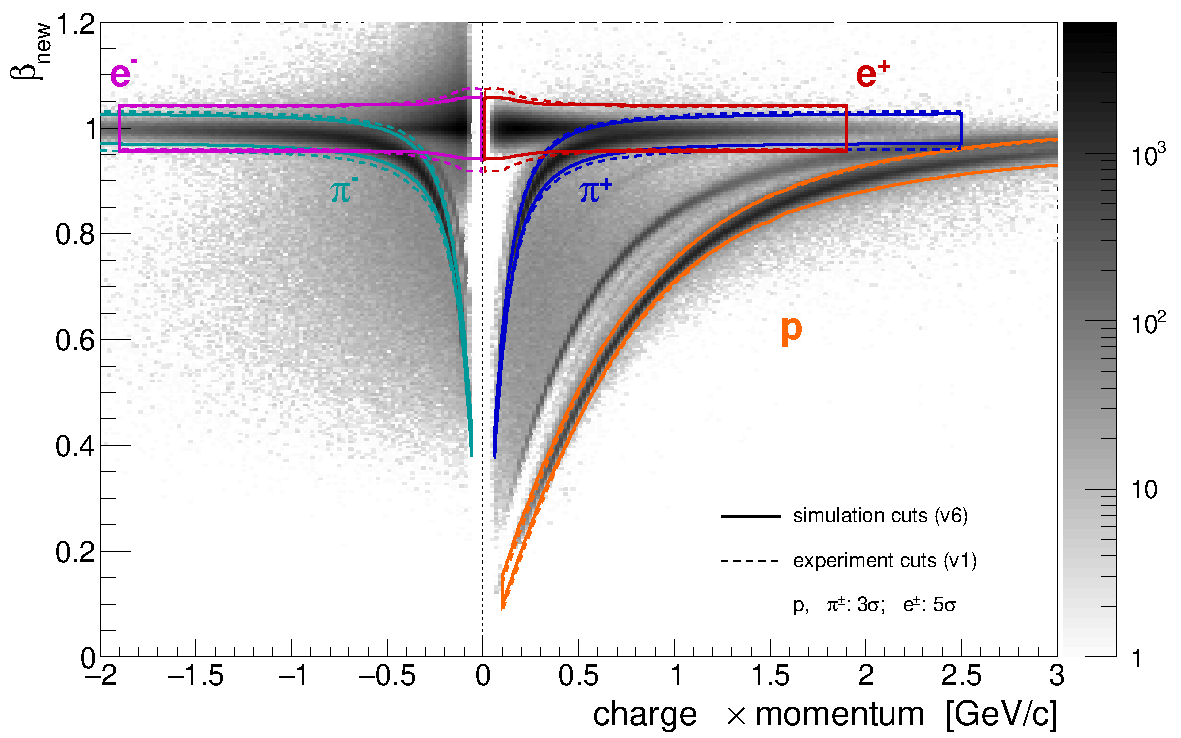
\includegraphics[width=\textwidth]{figs/banana_all.pdf}
\caption{$\betanew$ versus charge times momentum for simulated tracks before the PID cut
(SMASH p+p at 4.5\,GeV, no trigger condition, $\mathrm{isBest}=1$, vertex $z>-500$\,mm). Selection: simulated tracks of SMASH p+p at 4.5\,GeV before the PID cut; only the best-ranked combination of each event (isBest\,$=1$); a reconstructed event vertex ($z>-500$\,mm); no trigger condition, no target-region cut, unweighted; protons and pions: all tracks of the p, \pip and \pim slots of the hypothesis p\pip\pim (hadron PID sample \code{HH_elossfix}, 150 of 1000 files); $e^\pm$: all tracks of the $e^+$ and $e^-$ slots of the lepton PID sample (\code{LEP_merged}, 101 files), hypothesis \ppee, whose lepton slots hold only tracks with a correlated RICH ring and whose pion slots hold tracks without one.
Protons and pions: hadron PID sample, slots of the hypothesis p\pip\pim (\code{HH_elossfix},
150 of 1000 files); $e^\pm$: lepton PID sample, lepton slots of the hypothesis \ppee
(\code{LEP_merged}, 101 files). Solid lines: simulation cuts (v6), dashed: experiment cuts
(v1); p and $\pi^\pm$ at $3\sigma$, $e^\pm$ at $5\sigma$. The weak band between the \pip and the
proton bands is made of protons in the \pip slot and of \pip in the proton slot
(see the text).}
\label{fig:banana}
\end{figure}

\textbf{Electrons without a RICH ring in the \pim slot.} In Fig.~\ref{fig:leptons} a second band runs
to the right of the \pim band, almost parallel to the \pim cut. It is made of electrons in the \pim
slot (Fig.~\ref{fig:pimslot}). A lepton slot takes only tracks with a correlated RICH ring
(Sect.~\ref{sec:ana}); an electron without one is treated as a hadron and can occupy the \pim slot.
Measured with the pion mass, it follows Eq.~(\ref{eq:half}) derived below, $1/\betanew = \tfrac12(1/\beta_e + 1/\beta_\pi)$.
The most probable $\betanew$ of these electrons is 0.76, 0.90 and 0.97 at $p = 0.1$, 0.2 and
0.4\,\GeVc (expected 0.74, 0.90, 0.97), while the \pim band lies at 0.61, 0.82 and 0.94. Muons
in the \pim slot (5\,\%) are shifted much less (0.846 against 0.821 at 0.2\,\GeVc) and lie mostly inside the
\pim cut.

These electrons are not a small effect: before the PID cut they are 16\,\% of the \pim slot (72\,769 of
456\,971 tracks), and the \pim cut keeps 23\,\% of them. This agrees with the 4.3\,\% of the entries of the
lepton-set \code{_ID} tree that have an electron in the \pim slot (bit 5 of \code{sim_flags}).
Table~\ref{tab:norich} compares them with the electrons that have a ring.

\begin{figure}[!htbp]
\centering
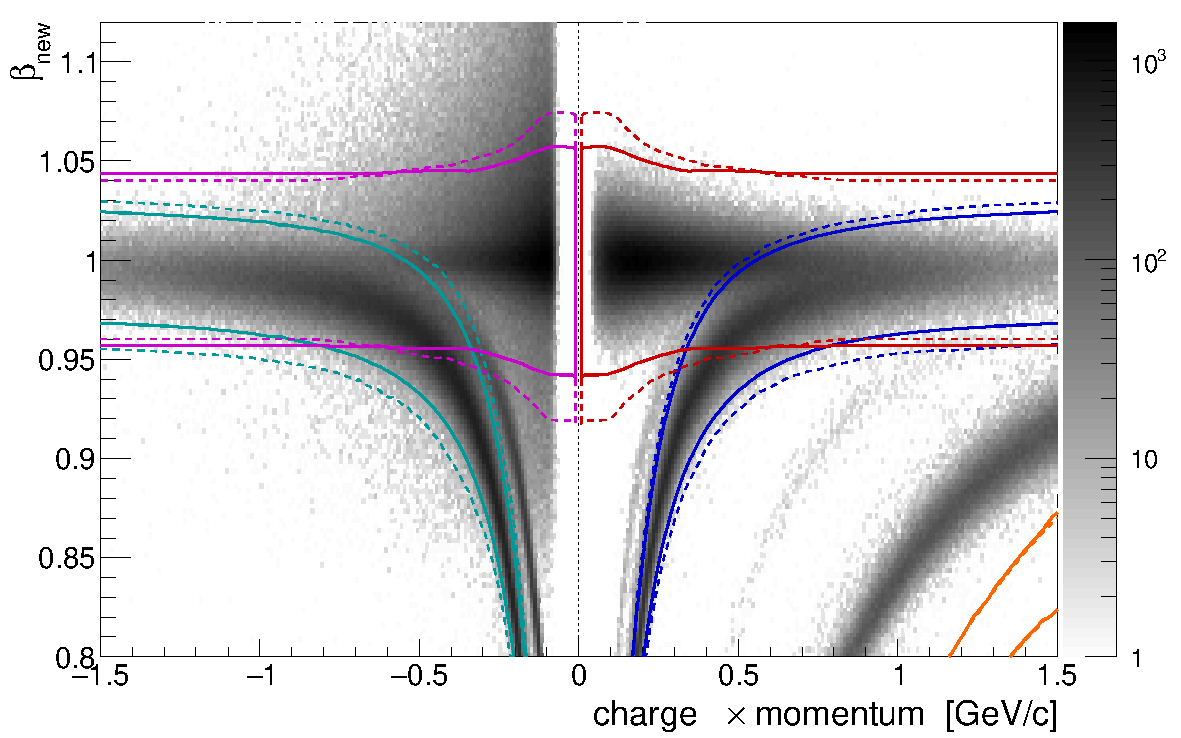
\includegraphics[width=0.93\textwidth]{figs/banana_leptons.pdf}
\caption{The lepton region of the \ppee hypothesis before the PID cut (all four slots,
lepton PID sample). Selection: simulated tracks of SMASH p+p at 4.5\,GeV before the PID cut; only the best-ranked combination of each event (isBest\,$=1$); a reconstructed event vertex ($z>-500$\,mm); no trigger condition, no target-region cut, unweighted; all tracks of the four slots (\pip, \pim, $e^+$, $e^-$) of the lepton PID sample (\code{LEP_merged}, 101 files), hypothesis \ppee, whose lepton slots hold only tracks with a correlated RICH ring and whose pion slots hold tracks without one; shown: $-1.5<$ charge $\times$ momentum $<1.5$\,\GeVc, $0.80<\betanew<1.12$. Above about 0.4\,\GeVc the pion bands enter the $e^\pm$ polygons: there
leptons are separated from pions by the RICH ring, not by $\betanew$. Lines as in
Fig.~\ref{fig:banana}.}
\label{fig:leptons}
\end{figure}

\begin{table}[!htbp]
\centering
\caption{Electrons without a RICH ring (in the \pim slot) and electrons with a ring (in the $e^-$
slot): GEANT creation process, parent particle and creation place, in percent of each group.
Lepton PID sample without PID cut, hypothesis \ppee, $\mathrm{isBest}=1$, vertex $z>-500$\,mm,
25 of the 101 files (18\,011 and 113\,135 electrons). Target region: $-200<z<-60$\,mm and $r<20$\,mm.
Macros \code{macros/norich.C}, \code{macros/norich_zr.C}; numbers in \code{tables/norich.txt}.}
\label{tab:norich}
\small
\begin{tabular}{@{}l r r@{}}
\toprule
 & $e^-$ in the \pim slot & $e^-$ in the $e^-$ slot \\
 & (no ring) & (ring) \\
\midrule
photon conversion ($\gamma\to\ee$)   & 86.6 & 35.2 \\
Compton scattering                    &  9.3 &  0.3 \\
knock-on (delta) electron             &  1.8 &  0.2 \\
decay (Dalitz decays of \piz, $\eta$) &  2.3 & 64.4 \\
\midrule
parent: photon / \piz / $\eta$        & 96.0 / 1.6 / 0.7 & 35.4 / 46.5 / 17.9 \\
\midrule
created in the target region          &  4.1 & 91.5 \\
created at $z = 200$--500\,mm          & 73.9 &  0.1 \\
created off the beam axis ($r>20$\,mm) & 95.8 &  7.7 \\
\midrule
ring found (\code{isring}) / lepton flag (\code{kIsLepton}) & 8.7 / 4.2 & 100 / 99.6 \\
ghost track (\code{sim_isghost})       & 29.2 & 8.9 \\
polar angle $\theta<18^\circ$          & 19.0 & 3.8 \\
\bottomrule
\end{tabular}
\end{table}

\begin{figure}[!htbp]
\centering
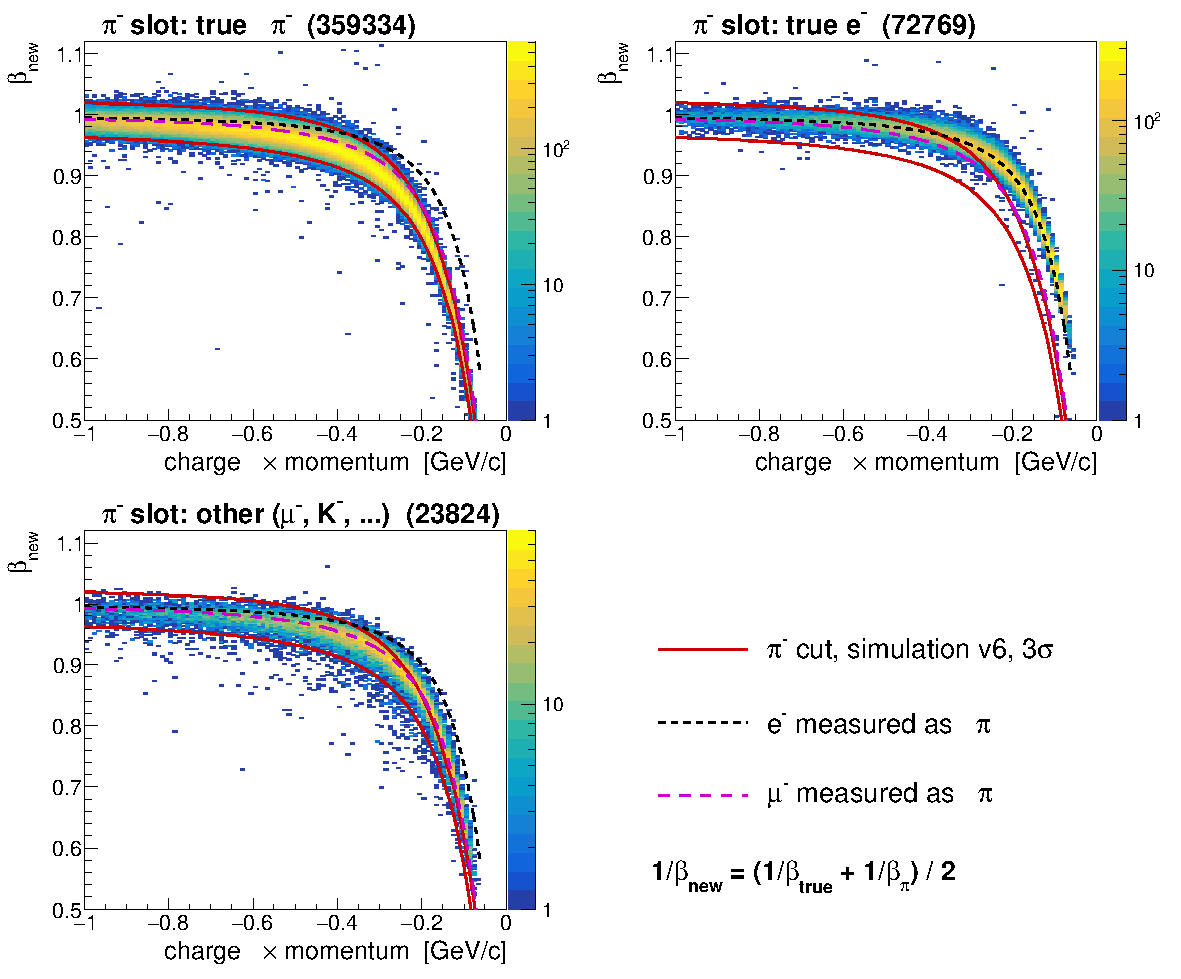
\includegraphics[width=0.92\textwidth]{figs/banana_pimslot.pdf}
\caption{The \pim slot of the \ppee hypothesis before the PID cut (lepton PID sample,
$\mathrm{isBest}=1$, vertex $z>-500$\,mm), split by the true particle: \pim, $e^-$, and the rest
(mostly $\mu^-$). Selection: simulated tracks of SMASH p+p at 4.5\,GeV before the PID cut; only the best-ranked combination of each event (isBest\,$=1$); a reconstructed event vertex ($z>-500$\,mm); no trigger condition, no target-region cut, unweighted; all tracks of the \pim slot of the lepton PID sample (\code{LEP_merged}, 101 files), hypothesis \ppee, whose lepton slots hold only tracks with a correlated RICH ring and whose pion slots hold tracks without one; split by the GEANT identity of the track. Red: \pim cut (simulation v6, $3\sigma$). Dashed: $\betanew$ expected for an electron
(black) and a muon (magenta) measured with the pion mass, Eq.~(\ref{eq:half}).}
\label{fig:pimslot}
\end{figure}

The electrons without a ring are secondary electrons of photons (mostly from \piz decays) produced
in the detector material \emph{downstream of the RICH radiator}:
\begin{itemize}
\item 28\,\% of their creation points lie within $\pm6$\,mm of a sphere of radius 872\,mm centred at
      $z\approx-625$\,mm. This is the RICH mirror: in the HGeant geometry (\code{rich.geo}) its radius is
      871--873\,mm and its centre is at $z = -532.2 - 88.5 = -620.7$\,mm. These are conversions in the
      mirror itself (carbon and glass segments).
\item Most of the others are created at $z\approx350$--500\,mm and $r\approx150$--350\,mm, about 0.6\,m
      from the target, which is the region of the first drift chambers (MDC~I). This attribution is
      inferred from the position; the HGeant medium numbers were not translated into material names.
\end{itemize}
They do not cross the \chem{C_4F_{10}} radiator, so they emit no Cherenkov light there: the missing
ring is expected and is not an inefficiency of the RICH. They still leave inner MDC segments and are
reconstructed as tracks.

\textbf{Charge asymmetry.} Ring-less positrons are rare: 0.6\,\% of the \pip slot against 16\,\% of
electrons in the \pim slot. This is not an effect of the hypothesis topology. In the hadron PID
sample without PID cut (hypothesis \pip\pim, \emph{all} combinations of 542\,211 events, every
distinct ring-less track counted once per event) the tracks created outside the target region give
$e^+ : e^- = 2\,633 : 24\,751$, a ratio of 0.106 (Table~\ref{tab:asym}). The ratio depends little on
the momentum but strongly on the polar angle. Of the conversion pairs, the positron partner of a
reconstructed electron is found in only 4.4\,\% of the cases, the electron partner of a reconstructed
positron in 38\,\%; both charges have the same ghost fraction (30--32\,\%), so the pair is not merged
into one track: the positron is lost. This agrees with the acceptance in the toroidal field: positive
particles are bent towards small polar angles and leave the acceptance, negative ones are bent
outwards. The strong dependence on $\theta$ supports this; the asymmetry that remains at large
$\theta$ and high momentum is not yet fully understood.

\begin{table}[H]
\centering
\caption{Ring-less $e^+$ (in the \pip slot) and $e^-$ (in the \pim slot) created outside the target
region, hadron PID sample without PID cut (\code{HH_elossfix}, 60 files, all combinations, each
track counted once per event; macro \code{macros/asym.C}).}
\label{tab:asym}
\small
\begin{tabular}{@{}l r r r@{\qquad}l r r r@{}}
\toprule
true $p$ [\MeVc] & $e^+$ & $e^-$ & $e^+/e^-$ & $\theta$ [deg] & $e^+$ & $e^-$ & $e^+/e^-$ \\
\midrule
0--100    & 302 & 1\,843 & 0.164 & $<20$  & 157 & 6\,814 & 0.023 \\
100--200  & 750 & 8\,403 & 0.089 & 20--30 & 585 & 6\,654 & 0.088 \\
200--300  & 564 & 5\,086 & 0.111 & 30--50 & 1\,125 & 7\,974 & 0.141 \\
300--500  & 551 & 5\,202 & 0.106 & 50--90 & 766 & 3\,309 & 0.231 \\
$>500$    & 466 & 4\,217 & 0.111 & & & & \\
\midrule
all       & 2\,633 & 24\,751 & 0.106 & & & & \\
\bottomrule
\end{tabular}
\end{table}

\textbf{Which cuts remove them.} After the PID cut, in the analysis ntuple of the standard set
(rules v2, base selection, $z>-160$\,mm), electrons are 2.5\,\% of the \pim slot (5\,464 entries); almost
all have $p>300$\,\MeVc, where the $\betanew$ bands of electrons and pions overlap, 95\,\% are
created at $z>100$\,mm and 90\,\% are conversions. Table~\ref{tab:eminpim} gives the fraction of
pions and electrons kept by candidate cuts.
\begin{itemize}
\item \textbf{Vertex cuts do not help:} a conversion electron continues in the direction of its
      photon, which came from the target, so its track points back to the vertex. The use in the
      vertex fit, the distance $|z_{\mathrm{trk}}-z_{\mathrm{vtx}}|$ and the distance $r$ from the beam
      axis keep electrons as often as pions.
\item \textbf{The energy loss in the MDC separates them:} median 2.75 for these electrons against 1.56
      for pions. A cut at 2.2 keeps 91.5\,\% of the pions and 15\,\% of the electrons, and lowers the
      electron share of the \pim slot from 2.5 to 0.4\,\%. Below 300\,\MeVc it keeps only 79\,\% of the
      pions (their energy loss rises), so a momentum-dependent cut is preferable.
\item Track $\chi^2$ and the angle to the nearest other track remove only about a quarter of them.
\end{itemize}
\emph{Not yet checked:} whether the MDC energy loss of simulation agrees with data, and whether the
high energy loss of these electrons is the relativistic rise or the double deposit of a close pair.

\begin{table}[H]
\centering
\caption{Fraction of true \pim and of electrons in the \pim slot kept by candidate cuts, analysis
ntuple \code{scan_nt} of the standard set (rules v2, after the PID cut, $z>-160$\,mm; macro
\code{macros/eminpim_cuts.C}; the lepton set gives the same picture). Numbers in
\code{tables/eminpim.txt}.}
\label{tab:eminpim}
\small
\begin{tabular}{@{}l c c c c@{}}
\toprule
 & \multicolumn{4}{c}{kept: \pim\ /\ $e^-$} \\
Cut & $p<300$\,\MeVc & 300--600\,\MeVc & $\ge600$\,\MeVc & all \\
\midrule
entries (\pim\ /\ $e^-$) & 54\,891 / 67 & 85\,475 / 3\,508 & 74\,669 / 1\,889 & 215\,035 / 5\,464 \\
\midrule
track used in the vertex fit & & & & 0.932 / 0.947 \\
$|z_{\mathrm{trk}}-z_{\mathrm{vtx}}|<20$\,mm & & & & 0.860 / 0.834 \\
$r<10$\,mm & & & & 0.938 / 0.949 \\
MDC $dE/dx<2.2$ & 0.787 / 0.373 & 0.965 / 0.165 & 0.951 / 0.105 & 0.915 / 0.147 \\
MDC $dE/dx<2.0$ & 0.679 / 0.239 & 0.921 / 0.058 & 0.891 / 0.035 & 0.849 / 0.053 \\
track $\chi^2<50$ & 0.886 / 0.851 & 0.920 / 0.769 & 0.949 / 0.790 & 0.921 / 0.777 \\
no track within 2$^\circ$ & 0.939 / 0.716 & 0.949 / 0.743 & 0.962 / 0.739 & 0.951 / 0.742 \\
\bottomrule
\end{tabular}
\end{table}

\textbf{$\betanew$ depends on the mass hypothesis of the track.} The relative-time method
(\code{HTimeCut}) takes one track $r$ of the combination as the time reference: an $e^-$ if
there is one, otherwise a proton, and among several candidates the one with the smallest
$\chi^2$. For every other track $j$ it uses the time
\begin{equation}
t_j^{\mathrm{new}} = t_j - \tfrac12\Big[\big(t_r - t_r^{\mathrm{exp}}\big) + \big(t_j - t_j^{\mathrm{exp}}\big)\Big],
\qquad \betanew = \frac{L_j}{c\,t_j^{\mathrm{new}}},
\label{eq:tnew}
\end{equation}
where $t$ is the measured time of flight, $t^{\mathrm{exp}} = L/(c\,\beta(p,m))$ the time
expected for the mass $m$ assumed in the hypothesis, and $L$ the path length. The start-time
correction is thus the average of the offsets $t - t^{\mathrm{exp}}$ of the reference and of
the track itself. For a track of the assumed mass the method gives its true velocity. For a
track of another mass half of the difference is absorbed; if the reference is correct,
\begin{equation}
\frac{1}{\betanew} = \frac12\left(\frac{1}{\beta_{\mathrm{true}}} + \frac{1}{\beta_{\mathrm{hyp}}}\right).
\label{eq:half}
\end{equation}
A proton of 1\,\GeVc in a \pip slot has $\betanew = 0.84$ instead of 0.73. A \pip in a proton
slot lands on the same curve, which is the weak middle band of Fig.~\ref{fig:banana}. The
reference track itself gets
$t_r^{\mathrm{new}} = t_r - \tfrac12(t_r - t_r^{\mathrm{exp}}) - \tfrac12\langle t_j - t_j^{\mathrm{exp}}\rangle_{j\neq r}$:
half of its own offset and half of the mean offset of its partners, so a wrongly assigned
partner shifts the velocity of the reference.

Figure~\ref{fig:hyp} shows what the PID cut acts on in this analysis: all four slots of the
\ppee hypothesis. The protons, which can only occupy the \pip and $e^+$ slots, form the band
of Eq.~(\ref{eq:half}) between the pion and the proton bands; only 7\,\% of them lie inside
the proton cut, and 2.6\,\% inside the \pip cut. Figure~\ref{fig:species} splits these tracks by
their true identity, and Table~\ref{tab:inside} gives the composition of each slot before the
PID cut together with the fraction of each kind of track inside the cut of the slot.

\begin{figure}[!htbp]
\centering
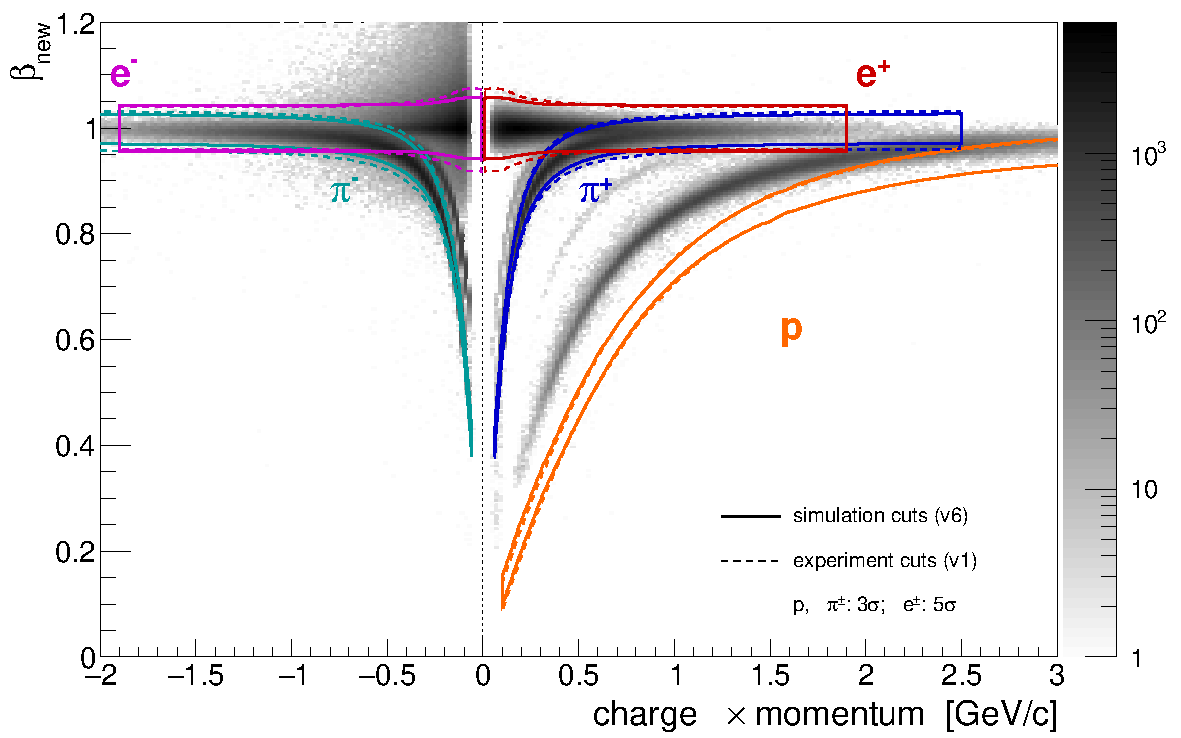
\includegraphics[width=\textwidth]{figs/banana_ppee.pdf}
\caption{All four slots of the \ppee hypothesis before the PID cut (lepton PID sample,
$\mathrm{isBest}=1$, vertex $z>-500$\,mm). Selection: simulated tracks of SMASH p+p at 4.5\,GeV before the PID cut; only the best-ranked combination of each event (isBest\,$=1$); a reconstructed event vertex ($z>-500$\,mm); no trigger condition, no target-region cut, unweighted; all tracks of the four slots (\pip, \pim, $e^+$, $e^-$) of the lepton PID sample (\code{LEP_merged}, 101 files), hypothesis \ppee, whose lepton slots hold only tracks with a correlated RICH ring and whose pion slots hold tracks without one. The protons appear in the \pip and $e^+$ slots,
measured with the pion or electron mass, halfway between the pion and the proton bands.
Lines as in Fig.~\ref{fig:banana}.}
\label{fig:hyp}
\end{figure}

\begin{figure}[!htbp]
\centering
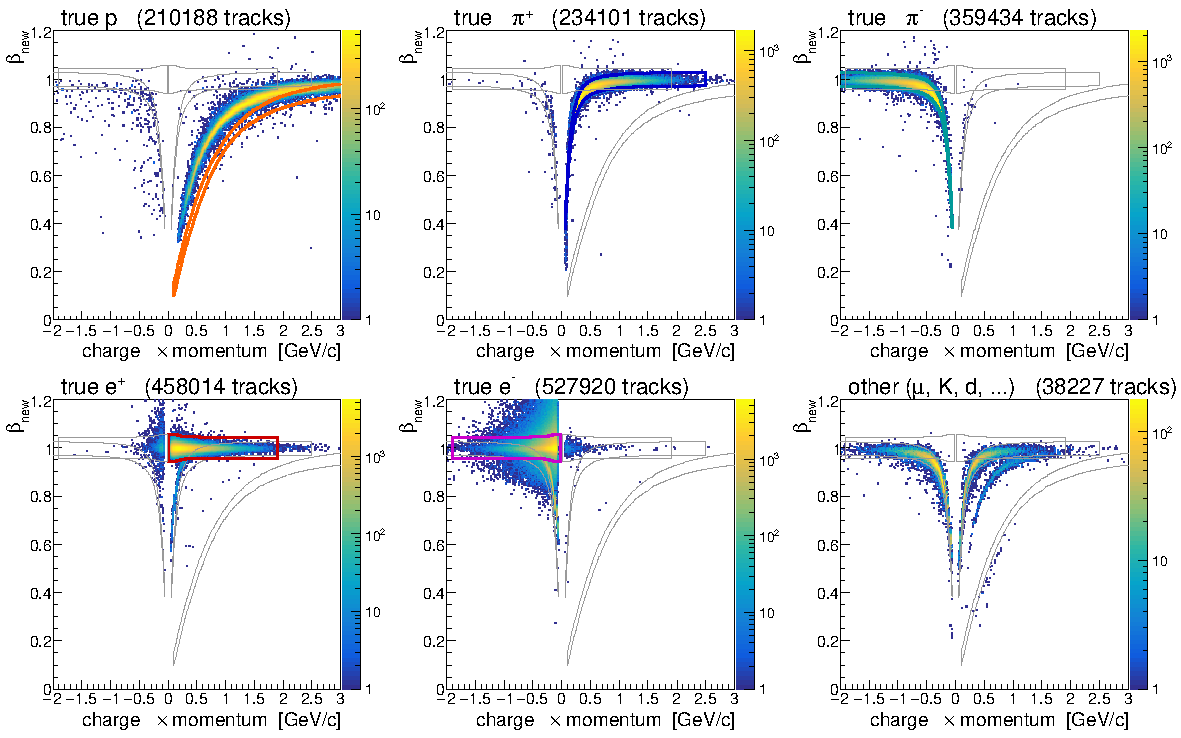
\includegraphics[width=\textwidth]{figs/banana_species.pdf}
\caption{The tracks of Fig.~\ref{fig:hyp} split by their true identity (GEANT). Selection: simulated tracks of SMASH p+p at 4.5\,GeV before the PID cut; only the best-ranked combination of each event (isBest\,$=1$); a reconstructed event vertex ($z>-500$\,mm); no trigger condition, no target-region cut, unweighted; all tracks of the four slots (\pip, \pim, $e^+$, $e^-$) of the lepton PID sample (\code{LEP_merged}, 101 files), hypothesis \ppee, whose lepton slots hold only tracks with a correlated RICH ring and whose pion slots hold tracks without one, split by the GEANT identity of the track (p, \pip, \pim, $e^+$, $e^-$). The coloured
polygon is the simulation cut of that species, the grey ones the other cuts.}
\label{fig:species}
\end{figure}

% generated by macros/rep_banana.C
\begin{table}[H]
\centering
\caption{Composition of the slots before the PID cut and the fraction of each kind of track that lies inside the simulation cut of its slot (v6; p, $\pi^\pm$ $3\sigma$, $e^\pm$ $5\sigma$). Each cell: share of the slot's tracks / fraction inside the cut. Simulation PID samples, $\mathrm{isBest}=1$, vertex $z>-500$\,mm, no trigger condition. Shares below 0.1\,\% are omitted.}
\label{tab:inside}
\footnotesize
\setlength{\tabcolsep}{4pt}
\begin{tabular}{@{}l r l l l l l l@{}}
\toprule
Hypothesis: slot & tracks & p & $\pi^+$ & $\pi^-$ & $e^+$ & $e^-$ & other \\
\midrule
p$\pi^+\pi^-$: p & 642804 & 0.889\,/\,0.936 & 0.104\,/\,0.010 & -- & -- & -- & 0.007\,/\,0.019 \\
p$\pi^+\pi^-$: $\pi^+$ & 642804 & 0.164\,/\,0.065 & 0.781\,/\,0.837 & -- & 0.005\,/\,0.228 & -- & 0.049\,/\,0.567 \\
p$\pi^+\pi^-$: $\pi^-$ & 642804 & -- & -- & 0.916\,/\,0.848 & -- & 0.032\,/\,0.254 & 0.051\,/\,0.636 \\
\midrule
$\pi^+\pi^-e^+e^-$: $\pi^+$ & 456971 & 0.453\,/\,0.026 & 0.510\,/\,0.988 & -- & 0.006\,/\,0.345 & -- & 0.031\,/\,0.682 \\
$\pi^+\pi^-e^+e^-$: $e^+$ & 456971 & 0.005\,/\,0.013 & 0.002\,/\,0.742 & -- & 0.991\,/\,0.999 & 0.002\,/\,0.989 & -- \\
$\pi^+\pi^-e^+e^-$: $\pi^-$ & 456971 & 0.002\,/\,0.313 & -- & 0.786\,/\,0.985 & -- & 0.159\,/\,0.228 & 0.052\,/\,0.668 \\
$\pi^+\pi^-e^+e^-$: $e^-$ & 456971 & -- & -- & -- & 0.005\,/\,0.840 & 0.994\,/\,0.837 & -- \\
\bottomrule
\end{tabular}
\end{table}


What the table shows:
\begin{itemize}
\item In the \ppee hypothesis the reference is the $e^-$, and the $e^-$ slot is 99.4\,\%
      pure. Correctly assigned pions and positrons then lie inside their cuts at the level
      expected from the cut widths: 98.8\,\% (\pip), 98.5\,\% (\pim), 99.9\,\% ($e^+$).
\item The $e^-$ itself, being the reference, is inside its cut only at 83.7\,\%: before the PID
      cut 45\,\% of the \pip slots hold a proton, and such a partner shifts the time of the
      reference. After the PID cut, when all partners must be inside their bands, this effect is
      much smaller.
\item In the p\pip\pim hypothesis there is no $e^-$, so the proton slot is the reference. With
      10\,\% \pip in the proton slot and 16\,\% protons in the \pip slot, even correctly assigned
      tracks lie inside their cuts at only 84--94\,\%.
\item Wrongly assigned tracks are mostly rejected: protons in a \pip slot pass the \pip cut at
      2.6\,\% (\ppee) and 6.5\,\% (p\pip\pim), \pip in a proton slot pass the proton cut at
      1.0\,\%.
\end{itemize}
The PID cut efficiency of a track therefore depends on its partners. Efficiencies have to be
taken from complete combinations, as the analysis does with the \code{_ID} trees and the GEANT
truth, and not from the width of single-track bands.

\subsection{Selection}
\label{sec:sel}
The base selection (``pre'') is common to all studies:
\begin{enumerate}
\item all combinations that passed the PID cuts, $\mathrm{isBest}\ge0$;
\item a reconstructed event vertex, $z>-500$\,mm (mandatory; later, Part~III: in the simulation it keeps 0.9997 of the
      direct decays, in the data $0.994\pm0.021$ of the $\eta$ but only 0.68 of the \ee counts, because the data counts without a
      vertex are mostly not hydrogen events (probably from upstream of the target cell, a hypothesis), which the simulation does not contain; \S\ref{sec:resnotdet});
\item the PT3 trigger (data: \code{trigbit == 8192}; simulation: bit test, bit 8192 set; see below);
\item the target region, $z>-160$\,mm (the target spans $-152$ to $-98$\,mm at half
      maximum, the maximum is at $-131$\,mm);
\item momenta corrected for the energy loss for all four particles (in data the corrected
      \pim momentum is missing for 0.7\,\% of the counts, \pim at $\theta<16^\circ$; such entries are
      dropped).
\end{enumerate}
On top of it the analysis studies the cuts of Table~\ref{tab:cuts}. Each of them is stored in
\code{scan_nt} both as a value and as a pass flag, so that every cut can be scanned and its
effect shown separately.

\textbf{The trigger PT3.} PT3, the main reaction trigger of the feb22 beam time, requires fullSecMult\,$\ge2$ and
iTOFPadMult\,$\ge3$: fullSecMult counts the sectors in which a hit of the inner TOF wall (iTOF) is in coincidence with a hit
of the TOF wall or of the RPC of the same sector, iTOFPadMult counts the hit iTOF paddles; in words, at least two sectors with
an inner-TOF hit in coincidence with TOF or RPC, and at least three inner-TOF paddles hit. PT2, the minimum-bias trigger,
requires fullSecMult\,$\ge1$ and is downscaled by 64. In the feb22 data only the bit of the trigger that arrives first is
written: PT3 events carry bit 8192, PT2 events and events with both PT2 and PT3 carry bit 4096, so the data events with bit 8192
hold 63/64 of all PT3 events (the data yields of Parts~II and III are multiplied by 64/63). Source: P.~Tlusty, ``LVL1 trigger
in Feb22 p+p 4.5\,GeV'', HADES internal presentation, 13 December 2024, with the definition slide of I.~Ciepa{\l}.
In the simulation the trigger bits are those written by the simulation production: a simulated PT3 event carries the value
$12288=8192+4096$ (both bits) and none carries 8192 alone, so the simulation condition is a bit test, \code{(trigbit & 8192) != 0}
(\S\ref{sec:tech}); the captions write it ``simulated PT3 trigger (bit 8192 set)''.

\begin{table}[H]
\centering
\caption{Cut variables of the analysis. All are computed from the corrected momenta.
The values are those of the named selections used so far; the cut scan of the data is
summarised in a later part.}
\label{tab:cuts}
\begin{tabularx}{\textwidth}{@{}l L l@{}}
\toprule
Variable & Meaning & Values used \\
\midrule
OA & opening angle of the \ee pair (lab) & $>2^\circ$ (conversions) \\
$\alpha_{\mathrm{lab}}$ & angle between the \pipi and the \ee systems (lab) & $<50^\circ$, 55, 40 \\
\Mpipi & invariant mass of the pions & $<0.42$, $<0.46$, $>0.30$\,\GeVcc \\
$\alpha_\eta$ & angle between \pipi and \ee in the rest frame of a hypothetical $\eta$ with the measured \ppee momentum and the mass $m_\eta$ (a band-pass in \Mfour) & $>140^\circ$ \\
pions in vertex & both pions used in the event-vertex fit (\code{isUsedVertex}) & flag \\
$\Delta z_\pi$ & $\max(|z_{\pi^+}-z_{\mathrm{vertex}}|, |z_{\pi^-}-z_{\mathrm{vertex}}|)$, $z$ of a track at its closest approach to the beam axis & $<40$\,mm \\
$\mathrm{MM}_4$, $p_{T,4}$ & missing mass of \ppee, the mass of (beam + target $-$ \ppee) four-momenta; transverse momentum of \ppee (lab) & studied \\
\bottomrule
\end{tabularx}
\end{table}

\begin{table}[H]
\centering
\caption{Named selections (all include ``pre'').}
\label{tab:presets}
\begin{tabular}{@{}l l@{}}
\toprule
Name & Cuts in addition to ``pre'' \\
\midrule
pre+OA$>2$ & OA $>2^\circ$ \\
slides & $\alpha_{\mathrm{lab}}<50^\circ$, $\Mpipi<0.46$\,\GeVcc, $\alpha_\eta>140^\circ$, OA$>2^\circ$ \\
old code & $\alpha_{\mathrm{lab}}<50^\circ$, $\Mpipi<0.42$\,\GeVcc, $\alpha_\eta>140^\circ$ \\
peak nominal & $\alpha_{\mathrm{lab}}<55^\circ$, $\Mpipi>0.30$\,\GeVcc \\
bump nominal & $\alpha_{\mathrm{lab}}<40^\circ$, $0.30<\Mpipi<0.41$\,\GeVcc \\
\bottomrule
\end{tabular}
\end{table}

\subsection{Software chain}
\begin{enumerate}
\item \textbf{PAT}, PostDST Analysis Tool (\code{git.gsi.de/przygoda/pat3}): DST $\to$ hypothesis ntuples with PID,
      relative-time reconstruction and ranking; simulation branch \code{pp45_sim_pippimepem}.
\item \textbf{FAT}, Final Analysis Tool (this repository, branch \code{pp45_pippimepem_betanew_sim}): base
      selection, kinematics, truth classes and weights (\code{src/sim_truth.h}), ntuple
      \code{scan_nt}; configurations \texttt{config\_sim\_\{std,lep,eta\}*.json}.
\item \textbf{Macros} (\code{plots/eta_sim/}): the common engine \code{SimEngine.h} (compact
      files, components, presets, weighted spectra with event-grouped errors) and the studies;
      figures in \code{plots/eta_sim/figs/}, tables in \code{plots/eta_sim/tables/}. Figures named \code{<name>_cnt.pdf} are redrawn by
      copies of their macros with the suffix \code{_cnt}, on the same inputs; only the word ``rows'' in their labels became ``counts''.
\end{enumerate}

% sec5_sim.tex -- Section "Simulation study: from the signal to the selection" of report_sim.tex
% (to be \input in place of the planned section 5). Simulation only. Macros: plots/eta_sim/s5_*.C,
% tables: plots/eta_sim/tables/s5_*.txt, figures: plots/eta_sim/figs/s5_*.pdf (copied to figs/).
%======================================================================
\section{Simulation study: from the signal to the selection}
\label{sec:simres}
%======================================================================
\inshort{on simulation alone the usual $\eta$ cuts do not raise the purity of the $\eta$ windows; the frozen selections
gain 4--5\,\% in $F$ over ``pre'' (bump: no cut); the template fit and the calibrated Gaussian fit recover the peak within
a few per cent, linear side bands lose 13--46\,\% (about 30\,\% on average); the expected X17 limit is
$1.9\times10^{-5}$ (preliminary), set by the simulation
statistics of the background. Later (Part~III): with realistic template noise the template fits come out about 10\,\% low
(\S\ref{sec:s5blind}); the X17 limit measured in the data is $3.16\times10^{-5}$ (PDG 2026; the frozen PDG 2020 value:
footnote~\ref{fn:x17pdg}; \S\ref{sec:s5x17}); in the simulation one third of the lost bump photons hit an active ECAL module
(\S\ref{sec:s5acc}).}
This section follows the order planned for the study (signal, acceptance, cuts, backgrounds,
optimisation, test of the extraction). It uses \textbf{simulation only}: no measured data were
read. The simulation contains no combinatorial background (CB), and none was added. All
statements about cuts therefore concern the physical background of SMASH, not the CB of the data.

\textbf{Common settings.} Every number of this section uses the same counts and weights:
\begin{itemize}
\item counts of the \ppee trees of the three sets (std, lep, $\eta$), owned in mode~A
      (Sect.~\ref{sec:weights});
\item the weight $W$ of Sect.~\ref{sec:weights} (PDG branching ratios) times the physics
      weights of the $\eta$ decays, main variant V3 (Sect.~\ref{sec:etagen}); for the bump the
      KLOE-2 Dalitz plot, for the conversion peak $|F_V|^2p^{*2}k^2$. All numbers of this section
      use the weight rules~v2 (exact HGeant branching ratios, Sect.~\ref{sec:hgeanteta});
\item the base selection ``pre'' (Sect.~\ref{sec:sel}); all cut variables from the corrected momenta;
\item cross section $\sigma = \sum W/\Lsim$ with $\Lsim = 221.05\,\nbinv$;
\item statistical errors from event groups: the variance of a sum is the sum over events of
      the squared sum of the weights of their counts. The effective number of simulated entries,
      $N_{\mathrm{eff}} = (\sum W)^2/\mathrm{Var}$, is quoted where it is small;
\item where a number of counts in the data is needed (significance, expected limits), the
      luminosity $\Ldata = 6080.5\,\nbinv$ (UNCONFIRMED) is used as a scale only: one unit of
      $\sum W$ corresponds to 27.51 expected counts.
\end{itemize}
The simulated sum is template T1 (signal classes 2--5) plus template T2 (physical background).
Templates T3 (fake lepton) and T4 (leptons from two sources) are never added; they are
shown separately and enter a background only as a stated variant. X17 counts (class~6) carry
$W = 2\,\mathrm{BR}$ per count, BR is a free parameter, and they are never added to the sum.
The windows in \Mfour and the background groups are the same in all parts
(Table~\ref{tab:s5defs}).

\begin{table}[H]
\centering
\caption{Windows in \Mfour and background groups used in this section. The peak window is
centred on the simulated peak ($0.5460\pm1.9\times0.0067$\,\GeVcc); the bump window is the
data bump window scaled by the simulated mass scale 1.0057. The groups split template~2 by the
lepton-pair class (L) and the pion-pair class (P) of \code{src/sim_truth.h} (all classes and the
templates T1--T4 are defined in Table~\ref{tab:classes}); a count goes to the first group in the order
given whose condition it fulfils.}
\label{tab:s5defs}
\small
\begin{tabularx}{\textwidth}{@{}l L@{}}
\toprule
Name & Definition \\
\midrule
peak window  & $0.5333 \le \Mfour < 0.5587$\,\GeVcc \\
bump window  & $0.4576 \le \Mfour < 0.5255$\,\GeVcc \\
other regions & below 0.4576; gap 0.5255--0.5333; 0.5587--0.70; 0.70--1.00; above 1.00\,\GeVcc \\
\midrule
classes 2, 3, 4, 5 & the signal classes (Table~\ref{tab:cls}): bump Dalitz, bump conversion,
   peak conversion, direct decay \\
$G_\eta$   & template 2 with both pions from one $\eta$ (P2) or an $\eta$ Dalitz pair (L2):
   an $\eta$ is produced, but the count is not a signal combination \\
$G_{\pi^0\mathrm{D}}$ & remaining template-2 counts with a \piz Dalitz pair (L1) \\
$G_{\mathrm{conv}}$ & remaining template-2 counts with a conversion pair (L3) \\
$G_{\mathrm{vec}}$  & remaining template-2 counts with $\rho^0,\omega,\phi\to\ee$, $\omega\to\piz\ee$
   or a second-decay pair (L4--L6) \\
$G_{\mathrm{oth}}$  & all other template-2 counts (in practice the \ee pair of a direct
   $\eta\to\ppee$ decay with pions from elsewhere) \\
$G_{\mathrm{fake}}$, $G_{\mathrm{diff}}$ & template 3 and template 4 (variants only) \\
multi-pion & $G_{\pi^0\mathrm{D}} + G_{\mathrm{conv}} + G_{\mathrm{vec}}$ \\
\bottomrule
\end{tabularx}
\end{table}

%----------------------------------------------------------------------
\subsection{The full spectrum and the cut sequence}
\label{sec:s5spec}
%----------------------------------------------------------------------
\inshort{the simulated sum after ``pre'' is $701.1\pm1.5$\,nb, 94\,\% of it multi-pion background; the four ``slides''
cuts remove background outside the $\eta$ windows, but inside them the purity does not rise and $F$ falls (peak
$52.1\to41.0$, bump $152.7\to112.5$).}
\textbf{The spectrum after ``pre''} (Fig.~\ref{fig:s5full}). The simulated sum is
$\sigma(\mathrm{T1+T2}) = 701.1\pm1.5$\,nb over all \Mfour. Of this, the four signal classes
are $14.89\pm0.27$\,nb and the multi-pion background $659.9\pm1.4$\,nb (94\,\%):
$G_{\pi^0\mathrm{D}} = 394.5\pm0.8$\,nb, $G_{\mathrm{conv}} = 265.3\pm1.2$\,nb and
$G_{\mathrm{vec}} = 0.107\pm0.001$\,nb. $G_\eta$ is $24.27\pm0.21$\,nb and $G_{\mathrm{oth}}$
$1.967\pm0.005$\,nb. Not in the sum: T3 $125.0\pm0.7$\,nb, T4 $12.51\pm0.25$\,nb. Above the
kinematic limit $\Mfour = \sqrt{s}-2m_p = 1.591$\,\GeVcc there are 2.87\,nb (0.4\,\%); 2.58\,nb
of them contain a misidentified track.

\begin{figure}[!htbp]
\centering
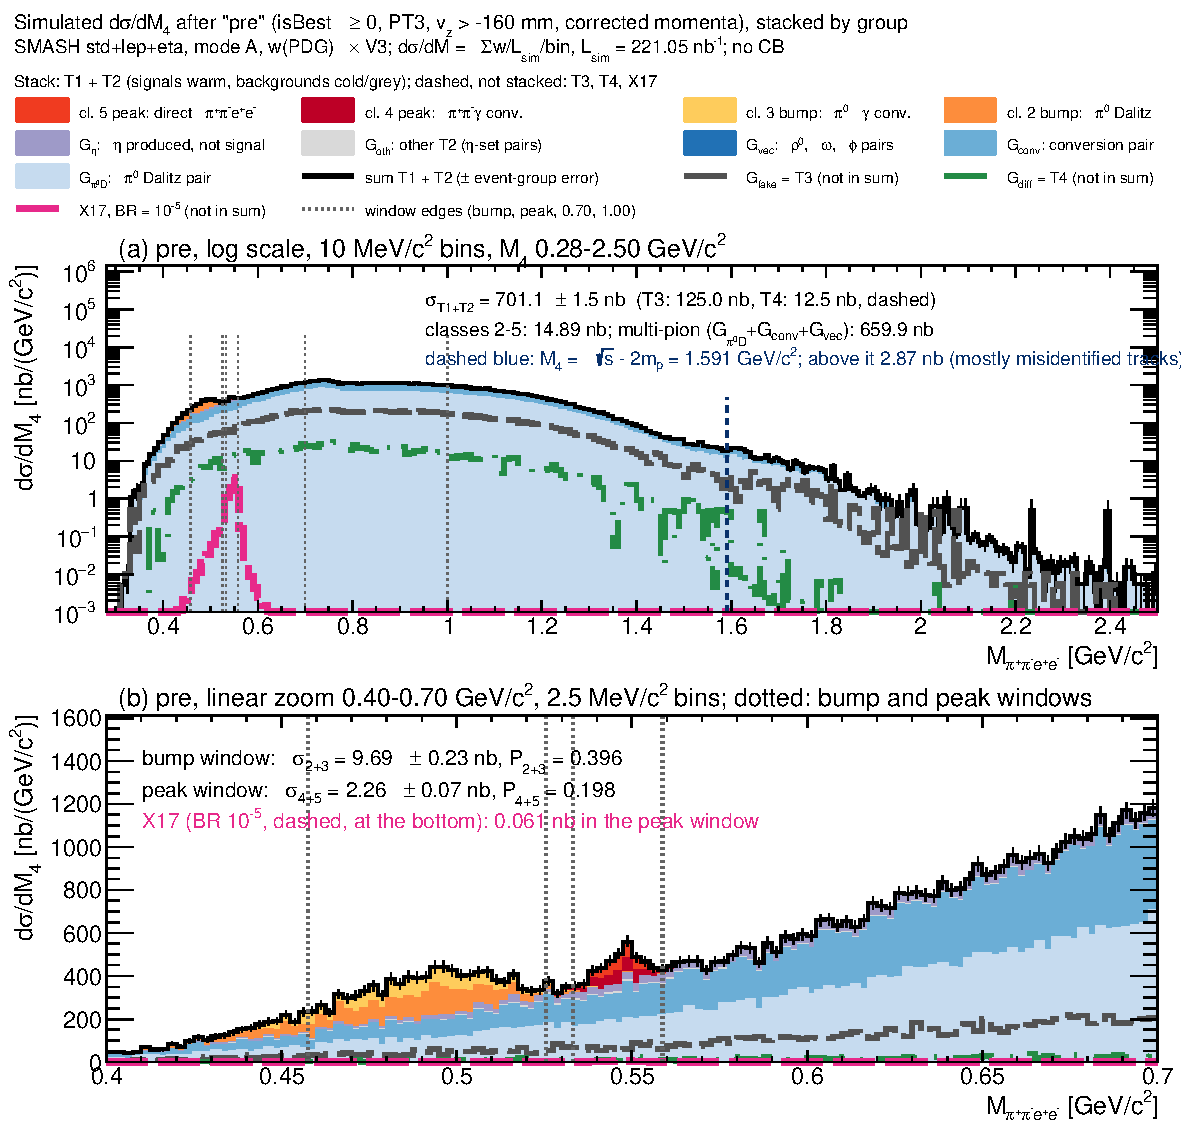
\includegraphics[width=\textwidth]{figs/s5_spec_full_pre.pdf}
\caption{Simulated $d\sigma/d\Mfour$ after ``pre'', stacked by group (signal classes warm,
background groups cold or grey). Selection: SMASH simulation only, no combinatorial background (standard, lepton and $\eta$ sets in mode~A; PDG branching ratios $\times$ the $\eta$-decay physics weights V3); base selection ``pre'' = simulated PT3 trigger (bit 8192 set), event vertex in the target region ($z>-160$\,mm), particle identification by \betanew with the simulation polygons (pions within $3\sigma$, leptons within $5\sigma$ and with a RICH ring), energy-loss-corrected momenta of all four tracks, all stored \ppee combinations per event (isBest\,$\ge0$); no further cut; all \Mee and \Mpipi; (a) $0.28\le\Mfour<2.50$\,\GeVcc, (b) $0.40\le\Mfour<0.70$\,\GeVcc; stacked: the signal classes 2--5 and the physical background (T1+T2); windows on the simulation mass scale: peak window $0.5333\le\Mfour<0.5587$\,\GeVcc, bump window $0.4576\le\Mfour<0.5255$\,\GeVcc. Dashed and not stacked: T3, T4 and X17 at
$\mathrm{BR} = 10^{-5}$. (a) Log scale, 10\,\MeVcc bins; the dashed blue line is the kinematic
limit. (b) Linear zoom, 2.5\,\MeVcc bins, with the bump and peak windows (dotted).}
\label{fig:s5full}
\end{figure}

\textbf{The cut sequence.} The four $\eta$-selection cuts of the analysis are applied one after
the other: $\mathrm{OA}>2^\circ$, $\alpha_{\mathrm{lab}}<50^\circ$, $\Mpipi<0.46$\,\GeVcc,
$\alpha_\eta>140^\circ$. All four together are the selection ``slides''.
Table~\ref{tab:s5flow} gives the cross sections, the purity $P$ = (signal in the window)/(T1+T2 in
the window) and $F = S/\sqrt{S+B}$, with $S$ the signal counts and $B$ the other T1+T2 counts of the
window at \Ldata. Figure~\ref{fig:s5steps} shows the spectrum after each step.

\begin{table}[H]
\centering
\caption{Cut sequence (nominal order). $\sigma$ in nb, errors from event groups. $P$: purity in
the window. $F = S/\sqrt{S+B}$ at $\Ldata = 6080.5\,\nbinv$ (UNCONFIRMED); in brackets $F$ with
$B$ + T3 + T4. Columns: the cuts OA$>2^\circ$, $\alpha_{\mathrm{lab}}<50^\circ$, $\Mpipi<0.46$\,\GeVcc and
$\alpha_\eta>140^\circ$ added one by one; last column: the final selection with $\Mpipi<0.42$\,\GeVcc.}
\label{tab:s5flow}
\footnotesize
\setlength{\tabcolsep}{3pt}
\begin{tabular}{@{}l rrrrr r@{}}
\toprule
 & pre & +OA & +$\alpha_{\mathrm{lab}}$ & +$M_{\pi\pi}$ & +$\alpha_\eta$ & $M_{\pi\pi}<0.42$ \\
\midrule
T1+T2, all $M_4$        & $701.1\pm1.5$ & $476.4\pm1.1$ & $254.0\pm0.9$ & $89.6\pm0.5$ & $67.9\pm0.5$ & $53.0\pm0.4$ \\
classes 2--5, all $M_4$ & $14.89\pm0.27$ & $10.58\pm0.22$ & $10.10\pm0.22$ & $10.06\pm0.22$ & $7.60\pm0.18$ & 7.26 \\
\midrule
bump: classes 2+3      & $9.69\pm0.23$ & $6.88\pm0.20$ & $6.61\pm0.19$ & $6.61\pm0.19$ & $5.60\pm0.17$ & $5.59\pm0.17$ \\
bump: T1+T2            & $24.48\pm0.33$ & $17.93\pm0.28$ & $16.71\pm0.27$ & $16.71\pm0.27$ & $15.08\pm0.25$ & $14.84\pm0.25$ \\
bump: $P$              & $0.396\pm0.007$ & $0.383\pm0.008$ & $0.395\pm0.008$ & $0.395\pm0.008$ & $0.371\pm0.008$ & $0.377\pm0.008$ \\
bump: $F$              & $152.7\pm3.0$ & $126.6\pm3.0$ & $126.0\pm3.0$ & $126.0\pm3.0$ & $112.5\pm2.9$ & $113.2\pm2.9$ \\
                       & (143.2) & (119.3) & (119.0) & (119.0) & (106.2) & (106.9) \\
\midrule
peak: classes 4+5      & $2.26\pm0.07$ & $1.57\pm0.05$ & $1.40\pm0.05$ & $1.37\pm0.05$ & $1.37\pm0.05$ & $1.07\pm0.04$ \\
peak: T1+T2            & $11.45\pm0.18$ & $8.45\pm0.15$ & $6.97\pm0.14$ & $6.79\pm0.13$ & $6.79\pm0.13$ & $5.64\pm0.12$ \\
peak: $P$              & $0.198\pm0.006$ & $0.185\pm0.006$ & $0.201\pm0.007$ & $0.202\pm0.007$ & $0.202\pm0.007$ & $0.190\pm0.007$ \\
peak: $F$              & $52.1\pm1.5$ & $42.0\pm1.3$ & $41.5\pm1.4$ & $41.0\pm1.4$ & $41.0\pm1.4$ & $35.3\pm1.2$ \\
                       & (48.1) & (39.0) & (38.4) & (38.0) & (38.0) & (32.6) \\
\bottomrule
\end{tabular}
\end{table}

\begin{figure}[!htbp]
\centering
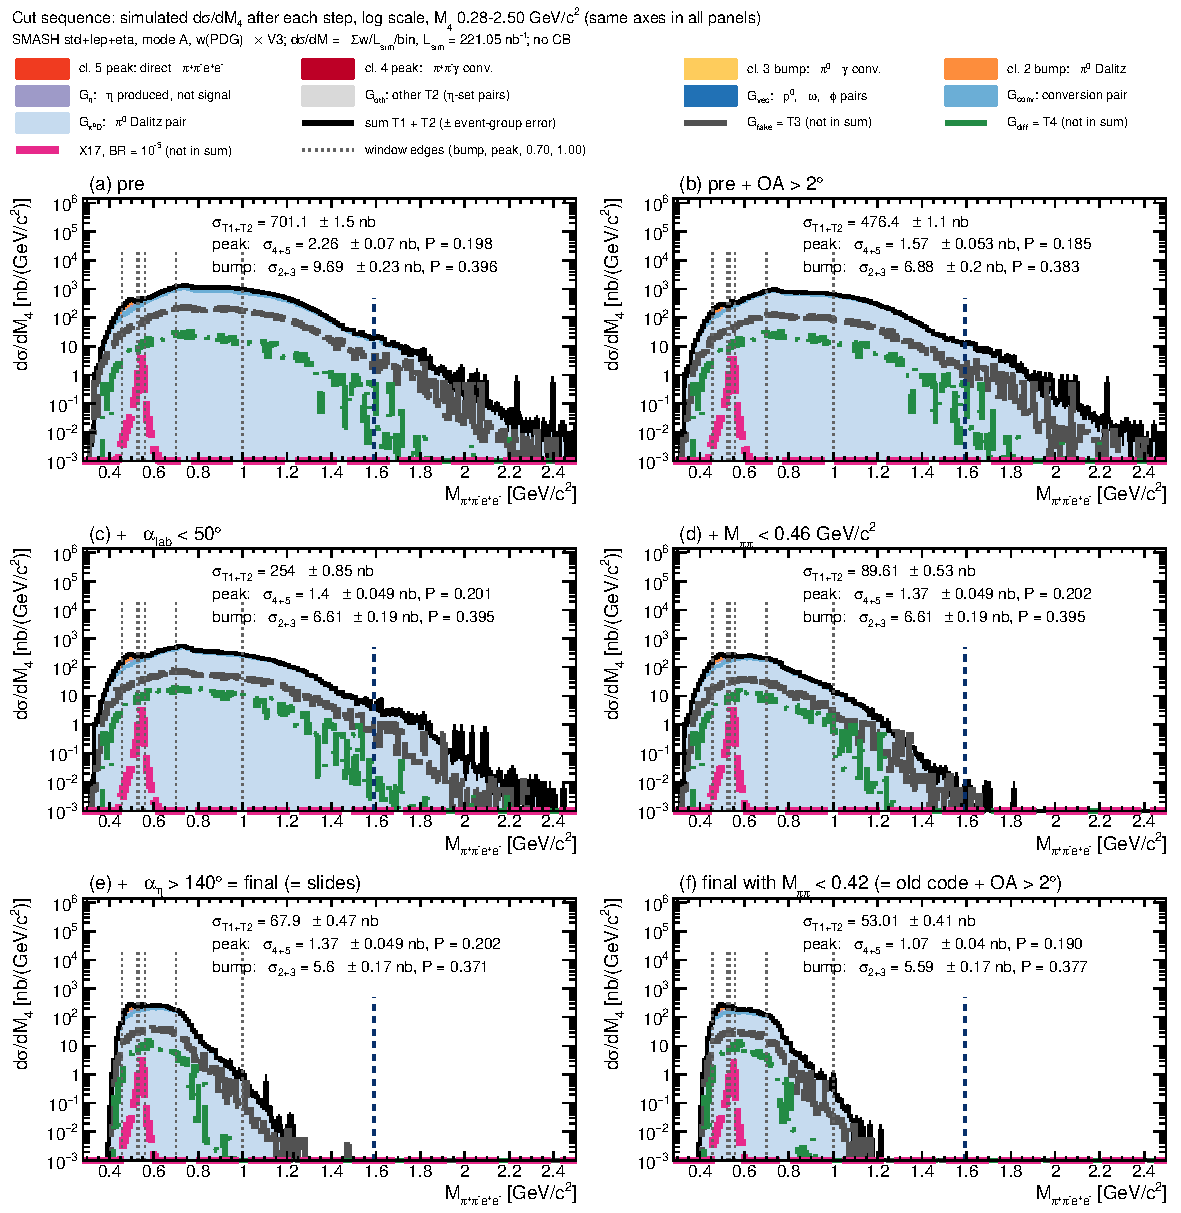
\includegraphics[width=\textwidth]{figs/s5_spec_steps_log.pdf}
\caption{Simulated $d\sigma/d\Mfour$ after each step of the cut sequence (same axes in all
panels; legend as in Fig.~\ref{fig:s5full}). Selection: SMASH simulation only, no combinatorial background (standard, lepton and $\eta$ sets in mode~A; PDG branching ratios $\times$ the $\eta$-decay physics weights V3); base selection ``pre'' = simulated PT3 trigger (bit 8192 set), event vertex in the target region ($z>-160$\,mm), particle identification by \betanew with the simulation polygons (pions within $3\sigma$, leptons within $5\sigma$ and with a RICH ring), energy-loss-corrected momenta of all four tracks, all stored \ppee combinations per event (isBest\,$\ge0$); $0.28\le\Mfour<2.50$\,\GeVcc in 10\,\MeVcc bins, all \Mee; (a) ``pre''; (b) (a) plus \ee opening angle above $2^\circ$ (OA); (c) (b) plus angle between the \pipi and \ee momenta in the laboratory below $50^\circ$ ($\alpha_{\mathrm{lab}}$); (d) (c) plus $\Mpipi<0.46$\,\GeVcc; (e) (d) plus the same angle in the rest frame of a hypothetical $\eta$ above $140^\circ$ ($\alpha_\eta$), i.e.\ ``slides''; (f) as (e) but with $\Mpipi<0.42$\,\GeVcc instead of 0.46 (``old code'' plus $\mathrm{OA}>2^\circ$). (a) pre; (b)--(e) the four cuts added one by one;
(e) is ``slides''; (f) the final selection with $\Mpipi<0.42$\,\GeVcc.}
\label{fig:s5steps}
\end{figure}

\textbf{Where each cut acts.} Table~\ref{tab:s5where} gives, for each cut applied alone to
``pre'', the fraction of the background of each \Mfour region that it removes.
\begin{itemize}
\item OA$>2^\circ$ removes 25--36\,\% of the background in every region: it acts everywhere the same.
\item $\alpha_{\mathrm{lab}}$ and \Mpipi act mainly above the $\eta$: \Mpipi$<0.46$ removes
      nothing in the bump window, because there $\Mpipi\le\Mfour-\Mee$ is already below the
      limit, and 1.8\,\% in the peak window.
\item $\alpha_\eta$ is a band-pass in \Mfour. It is the angle between \pipi and \ee in a frame
      obtained by boosting with the measured total momentum and an energy computed with the
      $\eta$ mass (\code{Physics::}\allowbreak\code{openingAngleInMassConstrainedRestFrame}). For
      $\Mfour = m_\eta$ this frame is the true rest frame and the angle is exactly $180^\circ$. In
      the peak window the cut therefore removes nothing (efficiency 1.000 for every group); it
      removes 75\,\% of the background below the bump, 78\,\% in 0.70--1.00 and 99\,\% above
      1.00\,\GeVcc, and 10--14\,\% of the bump signal in the bump window.
\end{itemize}

\begin{table}[H]
\centering
\caption{Fraction of the background removed by each cut alone (from ``pre''). Background: T1+T2
minus the signal of the window in the bump and peak windows, T2 elsewhere. Errors 0.002--0.012
in the first three columns, below 0.002 elsewhere.}
\label{tab:s5where}
\footnotesize
\setlength{\tabcolsep}{4pt}
\begin{tabular}{@{}l rrrrrr r@{}}
\toprule
cut & $<0.4576$ & bump & peak & 0.56--0.70 & 0.70--1.00 & $>1.00$ & all \Mfour (T2) \\
\midrule
OA$>2^\circ$                     & 0.247 & 0.252 & 0.250 & 0.276 & 0.317 & 0.363 & 0.321 \\
$\alpha_{\mathrm{lab}}<50^\circ$ & 0.014 & 0.077 & 0.166 & 0.307 & 0.473 & 0.559 & 0.455 \\
$\Mpipi<0.46$\,\GeVcc            & 0.000 & 0.0005 & 0.018 & 0.254 & 0.631 & 0.876 & 0.616 \\
$\alpha_\eta>140^\circ$          & 0.751 & 0.053 & 0.000 & 0.075 & 0.781 & 0.987 & 0.702 \\
\bottomrule
\end{tabular}
\end{table}

\textbf{The order of the cuts matters for the attribution.} Inside the two windows the cuts
act almost independently: the fraction attributed to a cut changes by 10--20\,\% (relative)
between the nominal and the reverse order. Over the whole spectrum it changes completely:
$\alpha_\eta$ removes 69\,\% of T1+T2 when applied first, but 3\,\% when applied last. A
statement ``this cut removes that much background'' is therefore meaningful only per window and
together with the order.

\textbf{The resulting shape.} After ``slides'' the multi-pion background is still the largest
part of every window: 0.72 below the bump, 0.55 in the bump window, 0.70 in the peak window,
0.89 in 0.56--0.70\,\GeVcc. T1+T2 above 0.70\,\GeVcc drops from 545.9 to 9.96\,nb, from 78\,\% to
15\,\% of the spectrum. Above 1.00\,\GeVcc only 0.037\,nb remain, with $N_{\mathrm{eff}} = 33$.

\notebox{\textbf{Main result of the spectrum study.} In the simulation the four cuts do not
raise the purity of either window (bump $0.396\to0.371$, peak $0.198\to0.202$), and $F$ falls at
every step (peak $52.1\to41.0$, bump $152.7\to112.5$). What the cuts do is remove the multi-pion
background outside the windows. A gain from these cuts in data can only come from what the
simulation does not contain: the CB, or a data/SMASH difference of the multi-pion background.
This must be checked with data. \emph{Later (Parts~II, III):} checked; the cuts do not help in the data either
(\S\ref{sec:s5data}, item~1).}

%----------------------------------------------------------------------
\subsection{The signal at generator level}
\label{sec:s5gen}
%----------------------------------------------------------------------
\inshort{the $\eta$ set holds $1.18\times10^{8}$ direct decays, i.e.\ $\sigma(pp\to\eta X) = 1.069$\,mb in SMASH; with
the physics weights the \Mee spectrum of the direct decay becomes much harder (31\,\% of the decays above 20\,\MeVcc
instead of 4.7\,\%).}
\textbf{Number of produced decays.} The PLUTO generator file of the $\eta$ set holds the true
kinematics of $N = 1\,181\,801$ direct decays from 1000 of the 100\,000 files. Assuming these
files are representative, the set contains $N_{\mathrm{direct}} = 100\,N = 1.1818\times10^{8}$
direct decays. Every $\eta$ of the set is forced, half into the direct decay, so the set holds
$N_\eta = 2N_{\mathrm{direct}} = 2.364\times10^{8}$ $\eta$ mesons, i.e.
$\sigma(pp\to\eta X) = N_\eta/\Lsim = 1.069$\,mb in SMASH. The decays of the other channels
are $N_\eta$ times the PDG branching ratio (Table~\ref{tab:s5prod}). The statistical error of
this scale is 0.09\,\%; whether the 1000 files are representative is UNVERIFIED. \emph{Later (Part~III):} an independent
count in 40 files gives $1.0690\pm0.0035$\,mb, a partial check; Part~III uses $N_\eta=2.364\times10^{8}$ (1.0694\,mb) for
the whole sample.

\begin{table}[H]
\centering
\caption{Produced decays per set ($10^{10}$ events) and production cross sections, from
$N_\eta$ and PDG branching ratios. Class 3 is counted per $\eta\to\pipi\piz$ decay with any \piz
decay (the conversion happens in the detector), class 4 per $\eta\to\pipi\gamma$ decay. Scale
error 0.09\,\% for every class.}
\label{tab:s5prod}
\small
\begin{tabular}{@{}l l r r@{}}
\toprule
Class & Channel & produced decays & $\sigma_{\mathrm{prod}}$ [nb] \\
\midrule
2 & $\eta\to\pipi\piz$, $\piz\to\ee\gamma$ & $6.360\times10^{5}$ & 2\,877.2 \\
3 & $\eta\to\pipi\piz$ (any \piz decay)     & $5.417\times10^{7}$ & 245\,075 \\
4 & $\eta\to\pipi\gamma$                    & $9.974\times10^{6}$ & 45\,123 \\
5 & $\eta\to\ppee$                          & $6.334\times10^{4}$ & 286.56 \\
6 & $\eta\to\pipi X17$, $X17\to\ee$, $\mathrm{BR}=10^{-5}$ & $2.364\times10^{3}$ & 10.693 \\
\bottomrule
\end{tabular}
\end{table}

\textbf{Shapes} (Fig.~\ref{fig:s5gen}). The physics weights replace the generator
distribution of the direct decay by Kroll--Wada $\times$ the P-wave rate $\times$ the form
factors $\times$ the decay angles (V3). The \Mee spectrum then becomes much harder:
\begin{center}
\small
\begin{tabular}{@{}l rrrrr@{}}
\toprule
fraction of produced decays with $\Mee >$ & 2 & 10 & 17 & 20 & 50\,\MeVcc \\
\midrule
direct, generator     & 0.513 & 0.099 & 0.057 & 0.047 & 0.016 \\
direct, V3            & 0.868 & 0.478 & 0.351 & 0.313 & 0.118 \\
bump \piz Dalitz (Kroll--Wada) & 0.860 & 0.443 & 0.308 & 0.268 & 0.070 \\
\bottomrule
\end{tabular}
\end{center}
The mean \Mpipi is 0.4007\,\GeVcc for the direct decay (V3), 0.3623 for the bump (KLOE-2; phase
space 0.3465), 0.4057 for the conversion peak ($|F_V|^2$; phase space 0.4014) and 0.3985 for X17
(three-body phase space, ASSUMED). The bump ends at $m_\eta-m_{\piz} = 0.413$\,\GeVcc.

\textbf{Direct decays under the X17 line.} The direct decay has a continuous \Mee spectrum and
contributes under any X17 line. With V3, the produced direct decays within $|\Mee-17| < d$ are
4.04, 7.95, 15.9 and 32.4\,nb for $d = 0.5$, 1, 2 and 4\,\MeVcc; X17 with
$\mathrm{BR}=10^{-5}$ is 10.69\,nb (Fig.~\ref{fig:s5gen}d).

\begin{figure}[!htbp]
\centering
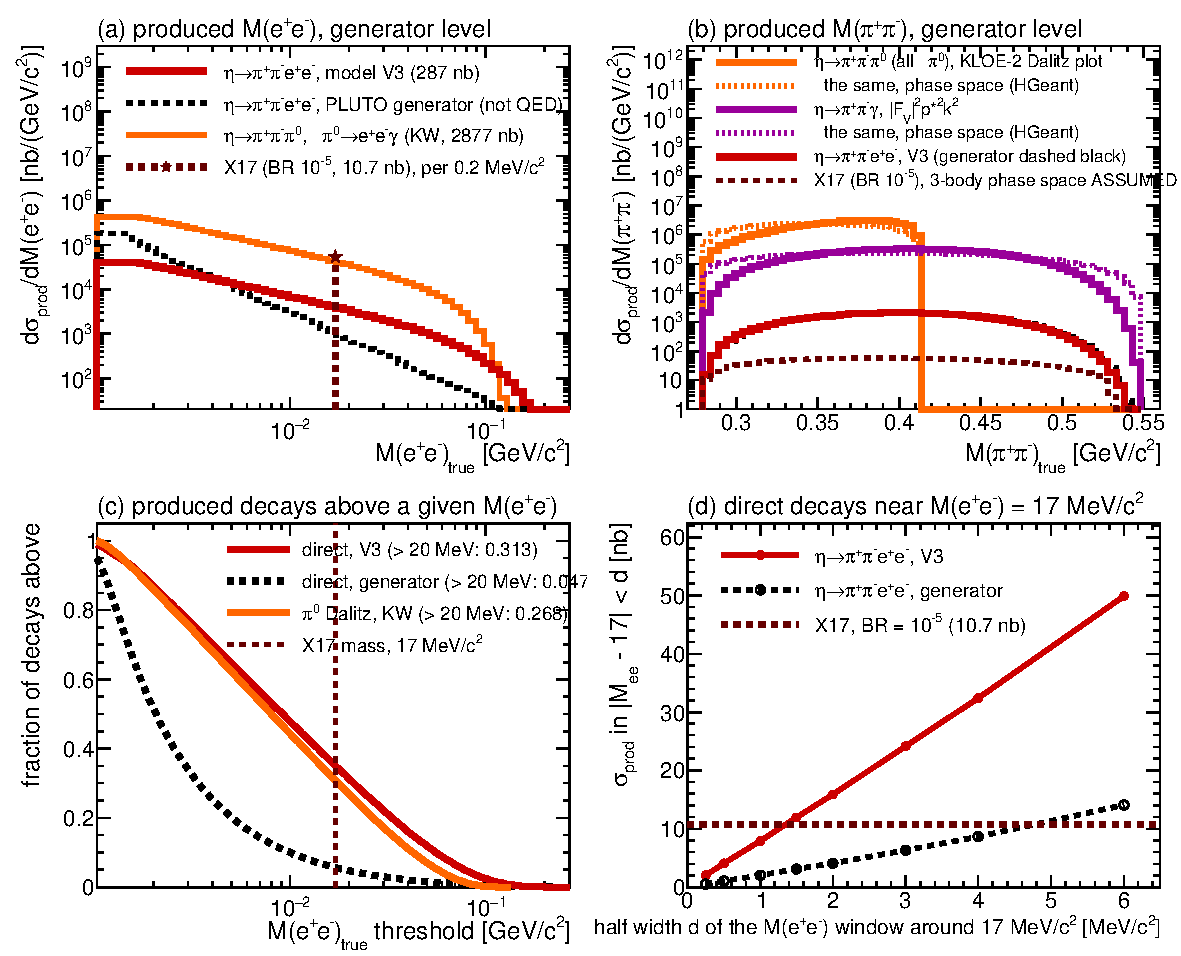
\includegraphics[width=\textwidth]{figs/s5_acc_gen.pdf}
\caption{Generator level, absolute scale ($\sigma_{\mathrm{prod}}$). Selection: none: all produced decays, before the detector simulation and before any cut; direct decays from the PLUTO generator sample of the $\eta$ set (1\,181\,801 decays in 1000 of the 100\,000 files, times 100), the other channels from their production densities (bump: HGeant phase space $\times$ KLOE-2 Dalitz plot; conversion peak: phase space $\times\,|F_V|^2p^{*2}k^2$; \piz Dalitz pair: Kroll--Wada; X17: three-body phase space, assumed); normalised with $N_\eta=2.364\times10^{8}$ $\eta$ mesons at $\Lsim=221.05\,\nbinv$. (a) \Mee of the direct decay
(V3 and generator), of the \piz Dalitz pair of the bump, and the X17 line. (b) \Mpipi of all
channels: physics models (solid) against the phase space of HGeant (dotted). (c) Fraction of
decays above a given \Mee. (d) Direct decays in a window $\pm d$ around 17\,\MeVcc against X17 at
$\mathrm{BR}=10^{-5}$.}
\label{fig:s5gen}
\end{figure}

%----------------------------------------------------------------------
\subsection{Acceptance and resolution}
\label{sec:s5acc}
%----------------------------------------------------------------------
\inshort{$\varepsilon$ of ``pre'' is 0.494\,\% for the direct decay, 0.667\,\% for X17, 0.245\,\% for the bump with a
\piz Dalitz pair and 0.002--0.003\,\% for the conversion classes; \Mfour is measured with a core width of
5.5--6.4\,\MeVcc and 0.22--0.39\,\% too low; the fixed peak window holds 0.851 of the simulated peak.}
\textbf{Acceptance $\times$ efficiency} $\varepsilon$ = (counts of the class after ``pre'', weighted)
/ (produced decays). Every accepted decay gives exactly one count of its class.
Table~\ref{tab:s5eps} gives the totals.

\begin{table}[H]
\centering
\caption{Acceptance $\times$ efficiency of ``pre'' per produced decay, in \%. Classes 3 and 4
include the conversion probability (per $\eta\to\pipi\piz$ and per $\eta\to\pipi\gamma$ decay).
X17: at $\mathrm{BR}=10^{-5}$.}
\label{tab:s5eps}
\footnotesize
\setlength{\tabcolsep}{4pt}
\begin{tabular}{@{}l rr r rr rr@{}}
\toprule
 & & & & \multicolumn{2}{c}{$\varepsilon$, all $M_4$} & \multicolumn{2}{c}{$\varepsilon$ (V3), window} \\
class & entries & $N_{\mathrm{eff}}$ & $\sigma_{\mathrm{acc}}$ [nb] & V3 & no weights & peak & bump \\
\midrule
5 direct    & 571\,246 & 171\,004 & $1.4168\pm0.0034$ & $0.4944\pm0.0013$ & 0.4834 & 0.4213 & 0.0249 \\
6 X17       & 787\,659 & 787\,653 & 0.0713 & $0.6665\pm0.0010$ & 0.6665 & 0.5714 & 0.0352 \\
2 bump Dalitz & 1\,649 & 1\,332 & $7.05\pm0.19$ & $0.245\pm0.007$ & 0.275 & 0.0010 & 0.194 \\
3 bump conv.  & 1\,187 &   948 & $5.19\pm0.17$ & $0.00212\pm0.00007$ & 0.00238 & 0 & 0.00167 \\
4 peak conv.  &   307 &   270 & $1.24\pm0.08$ & $0.00275\pm0.00017$ & 0.00272 & 0.00234 & 0.00013 \\
\bottomrule
\end{tabular}
\end{table}

\textbf{Later finding (Part~III).} The class-2 efficiency of Table~\ref{tab:s5eps} is too high: HGeant decays the
virtual photon of the \piz Dalitz decay isotropically instead of as $1+\cos^2\theta^*$ (see the notes in
Sect.~\ref{sec:weights}; Part~III, \code{report_all.pdf}). For the bump the full simulation gives the QED factor 0.86, so the
simulated efficiency is about 16\,\% too high (the toys and the closure of prompt \piz Dalitz pairs gave 12--14\,\%). It is
not corrected here; Part~III weights every simulated class-2 count of its bump-edge fits with the QED angle (its D38,
approved by the analyst on 15 November 2026).

Figure~\ref{fig:s5acc} shows $\varepsilon$ against the true \Mee and \Mpipi.
\begin{itemize}
\item \textbf{True \Mee} (direct decay, V3): 0.34--0.37\,\% at 2--4\,\MeVcc, 0.49\,\% at 10, 0.53\,\% at
      16--20, 0.58\,\% at 45--57, 0.96\,\% at 100--124 and 1.8--2.0\,\% above 160\,\MeVcc. A pair of
      small mass has a small opening angle and is often lost. The two lowest bins are affected by
      the stored precision of the generator file.
\item \textbf{Decay angles.} At fixed \Mee, V3 lowers $\varepsilon$ by the factor 0.82 at
      5--20\,\MeVcc and 0.84--0.90 at 20--75\,\MeVcc (Fig.~\ref{fig:s5acc}c). The cause is the QED
      $e^+$ angle $1+\cos^2\theta^*_e$: V2, the same model without the angles, changes $\varepsilon$
      by less than 6\,\%. Over all \Mee V3 still raises $\varepsilon$ by 2.3\,\%, because it moves
      decays to higher \Mee.
\item \textbf{True \Mpipi.} $\varepsilon$ falls steeply with \Mpipi, because a heavy pion pair leaves
      slow leptons: direct decay 0.86\,\% at 0.29--0.30, 0.47\,\% at 0.41--0.42, 0.016\,\% at
      0.49--0.50 and 0 above 0.52\,\GeVcc.
\item \textbf{X17 against the direct decay} at the same true \Mee (14--20\,\MeVcc): without physics
      weights the two agree within about 5\,\% below $\Mpipi = 0.45$\,\GeVcc (Fig.~\ref{fig:s5acc}d).
      This supports, but does not prove, the phase-space \Mpipi and the isotropic decay assumed
      for X17.
\end{itemize}

\begin{figure}[!htbp]
\centering
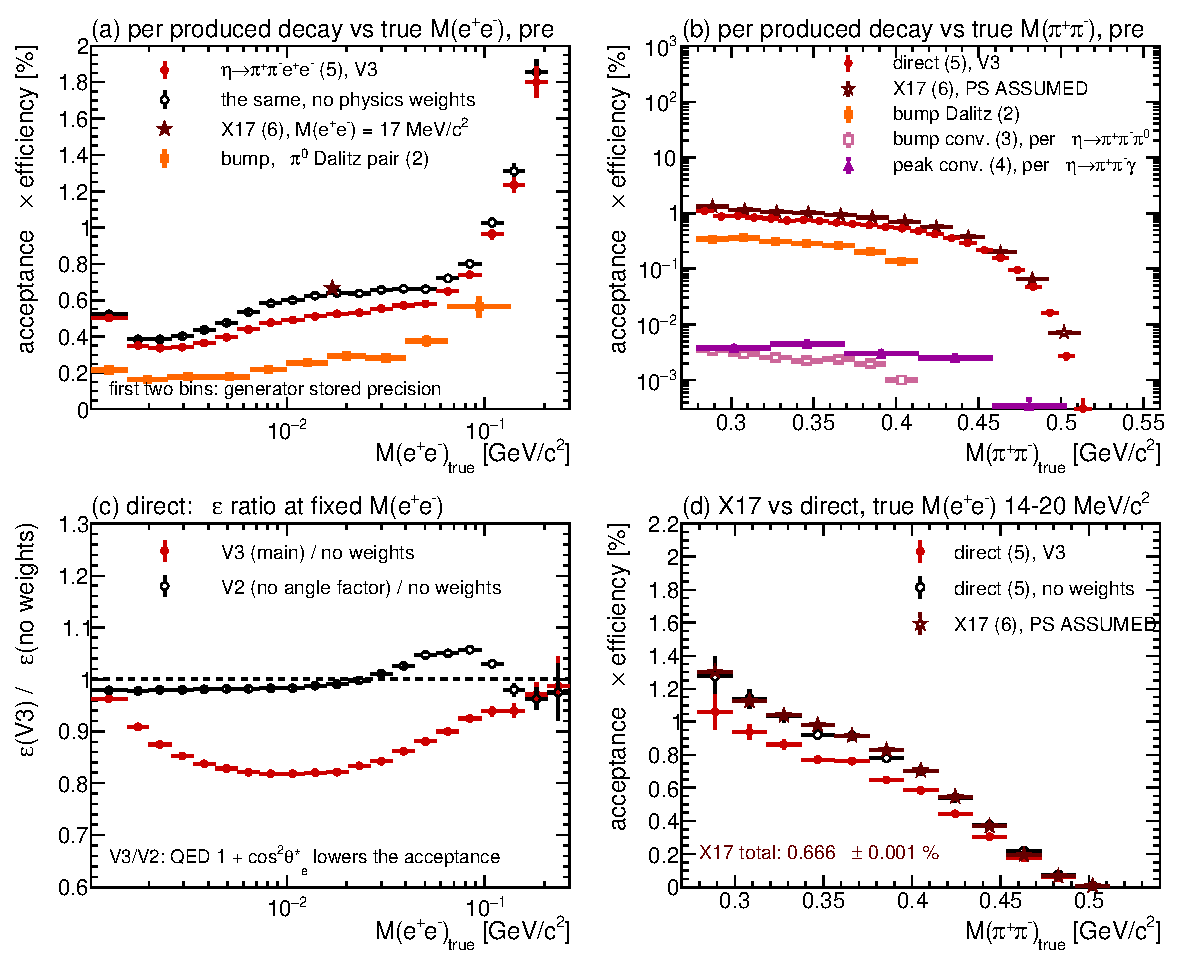
\includegraphics[width=\textwidth]{figs/s5_acc_eff_mass.pdf}
\caption{Acceptance $\times$ efficiency of ``pre'' per produced decay. Selection: SMASH simulation only, no combinatorial background (standard, lepton and $\eta$ sets in mode~A; PDG branching ratios $\times$ the $\eta$-decay physics weights V3); base selection ``pre'' = simulated PT3 trigger (bit 8192 set), event vertex in the target region ($z>-160$\,mm), particle identification by \betanew with the simulation polygons (pions within $3\sigma$, leptons within $5\sigma$ and with a RICH ring), energy-loss-corrected momenta of all four tracks, all stored \ppee combinations per event (isBest\,$\ge0$); numerator: weighted counts of each signal class after ``pre'' at all \Mfour, \Mee and \Mpipi (no window); denominator: produced decays of the same class at generator level (direct decay: generator sample $\times100$; class~2 per $\eta\to\pipi\piz$, $\piz\to\ee\gamma$ decay; class~3 per $\eta\to\pipi\piz$ decay; class~4 per $\eta\to\pipi\gamma$ decay); ``no weights'' = without the $\eta$-decay physics weights; (d) direct decays with true $14\le\Mee<20$\,\MeVcc, X17 all counts. (a) Against the true \Mee:
direct decay (V3 and without physics weights), bump \piz Dalitz pair, X17. (b) Against the true
\Mpipi for all classes. (c) Ratio V3/no weights and V2/no weights at fixed \Mee: the effect of the
decay angles. (d) X17 against the direct decay at true \Mee 14--20\,\MeVcc.}
\label{fig:s5acc}
\end{figure}

\textbf{Resolution and scale} (Table~\ref{tab:s5res}, Fig.~\ref{fig:s5res}). The difference
reconstructed minus true is fitted with a Gaussian core (iterated in $\pm2\sigma$); the tails are
counted outside $\pm3\sigma$. The reconstructed \Mfour is low by 0.22--0.39\,\% (median ratio)
and has a low-side tail from energy loss and radiation: 6\,\% of the direct decays lie more than
$3\sigma$ below the core. The \Mee resolution comes from the opening-angle measurement (OA
resolution 1.0--1.4$^\circ$): at 17\,\MeVcc the core width is $4.21\pm0.01$\,\MeVcc with a median
shift of $+0.10$\,\MeVcc; 90\,\% of the X17 counts lie in 9.7--24.3\,\MeVcc.

\begin{table}[H]
\centering
\caption{Resolution of \Mfour (reconstructed with corrected momenta minus true), after ``pre''.}
\label{tab:s5res}
\footnotesize
\setlength{\tabcolsep}{4pt}
\begin{tabular}{@{}l rr c r r@{}}
\toprule
 & \multicolumn{2}{c}{$\Delta M_4$ [\MeVcc]} & tail fraction & median & $\Delta M_{\pi\pi}$ core \\
class & median & core $\sigma$ & below / above $3\sigma$ & $M_4/M_{4,\mathrm{true}}$ & $\sigma$ [\MeVcc] \\
\midrule
5 direct      & $-2.12\pm0.02$ & $6.44\pm0.02$ & 0.057 / 0.014 & 0.99614 & $3.49\pm0.01$ \\
6 X17         & $-2.10\pm0.01$ & $6.25\pm0.01$ & 0.063 / 0.013 & 0.99617 & $2.98\pm0.01$ \\
2 bump Dalitz & $-1.47\pm0.22$ & $5.47\pm0.18$ & 0.041 / 0.015 & 0.99694 & $3.13\pm0.12$ \\
3 bump conv.  & $-1.05\pm0.27$ & $5.68\pm0.26$ & 0.033 / 0.020 & 0.99783 & $3.11\pm0.13$ \\
4 peak conv.  & $-1.33\pm0.57$ & $6.13\pm0.40$ & 0.060 / 0.008 & 0.99757 & $3.15\pm0.26$ \\
\bottomrule
\end{tabular}
\end{table}

\begin{figure}[!htbp]
\centering
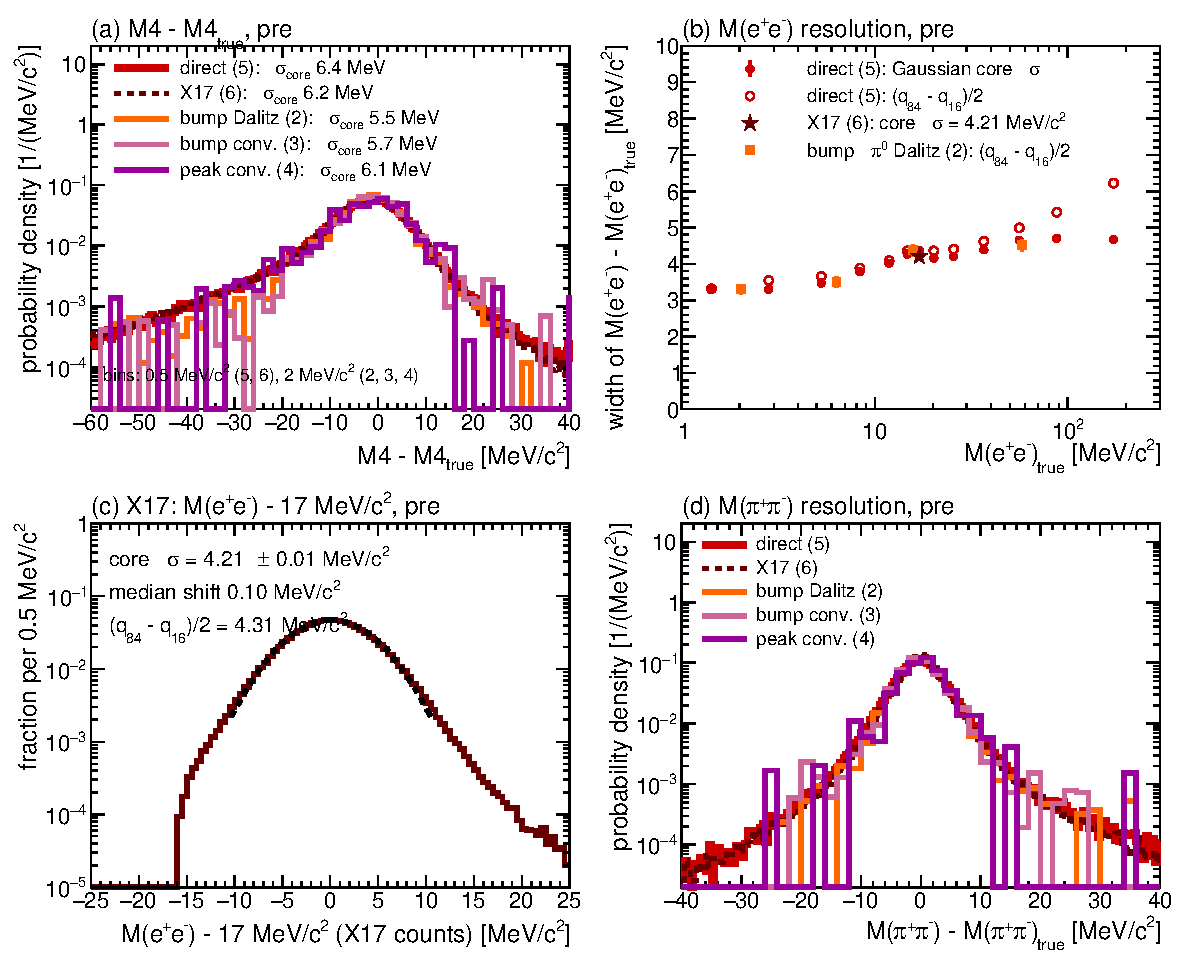
\includegraphics[width=\textwidth]{figs/s5_acc_res_cnt.pdf}
\caption{Resolution after ``pre''. Selection: SMASH simulation only, no combinatorial background (standard, lepton and $\eta$ sets in mode~A; PDG branching ratios $\times$ the $\eta$-decay physics weights V3); base selection ``pre'' = simulated PT3 trigger (bit 8192 set), event vertex in the target region ($z>-160$\,mm), particle identification by \betanew with the simulation polygons (pions within $3\sigma$, leptons within $5\sigma$ and with a RICH ring), energy-loss-corrected momenta of all four tracks, all stored \ppee combinations per event (isBest\,$\ge0$); all \Mfour (no window); reconstructed values (energy-loss-corrected momenta) minus the GEANT true values; (a) and (d) per signal class 2--6, (b) direct decay (class~5), X17 and the bump \piz Dalitz pair (class~2) in bins of the true \Mee, (c) all X17 counts. (a) $\Mfour-M_{4,\mathrm{true}}$ per class. (b) Width of
$\Mee-M_{ee,\mathrm{true}}$ against the true \Mee. (c) Reconstructed \Mee of the X17 counts minus
17\,\MeVcc. (d) $\Mpipi-M_{\pi\pi,\mathrm{true}}$.}
\label{fig:s5res}
\end{figure}

\textbf{Check of the peak window.} A Gaussian fit of the simulated peak (classes 4+5, V3, 1\,\MeVcc
bins, iterated in $\pm2\sigma$) gives $\mu = 0.54637\pm0.00020$\,\GeVcc and
$\sigma = 6.09\pm0.19$\,\MeVcc, so $\mu\pm1.9\sigma$ = 0.5348--0.5579\,\GeVcc. The fixed window
(0.5333--0.5587) is 1.5\,\MeVcc wider on the low side. Nine fit choices (bin width, fit range)
move the lower edge by $+0.1$ to $+3.2$\,\MeVcc; the direct decay alone ($N_{\mathrm{eff}}$ 171\,000)
reproduces the fixed window within 0.7\,\MeVcc. The fixed window is therefore kept. It holds 0.851
of the simulated peak, $2.262\pm0.070$\,nb (direct $1.207\pm0.003$, conversion $1.054\pm0.070$).

\emph{Later (Part~III):} the data $\eta$ peak sits at $0.54388\pm0.00049$\,\GeVcc, lower than the simulated 0.5460, and
is narrower, $5.44\pm0.60$ against 6.09\,\MeVcc (only $1.1\sigma$; it favours a resolution factor 0.89, which Part~III
treats as a systematic variant). Part~III scales every simulated \Mfour by $s=0.99615$ (from the two peak positions) and
every \Mpipi by 0.9952; the K$^0_S$ peak in \Mpipi then agrees with the data in position ($0.9997\pm0.0011$), while the
data width is 1.12--1.16 times the simulated one.

\textbf{The opening angle separates conversions only weakly.} The true OA of a conversion pair is
small (median 0.51$^\circ$), but the reconstructed OA is larger by about 1.6$^\circ$ (median
2.2$^\circ$), because of the OA resolution and the need for two separated tracks. The fraction with
OA$>2^\circ$ is 0.811 (direct), 0.955 (X17), $0.814\pm0.011$ (bump Dalitz), $0.576\pm0.016$ (bump
conversion) and $0.567\pm0.030$ (peak conversion). A cut on \Mee separates about as well:
$\Mee>15$\,\MeVcc keeps 0.50 of the direct decay and 0.02 of the conversion peak.
OA does not separate X17 from the direct decay at the same reconstructed \Mee (confirmed later by Part~III,
\S\ref{sec:s5x17}).

\begin{figure}[!htbp]
\centering
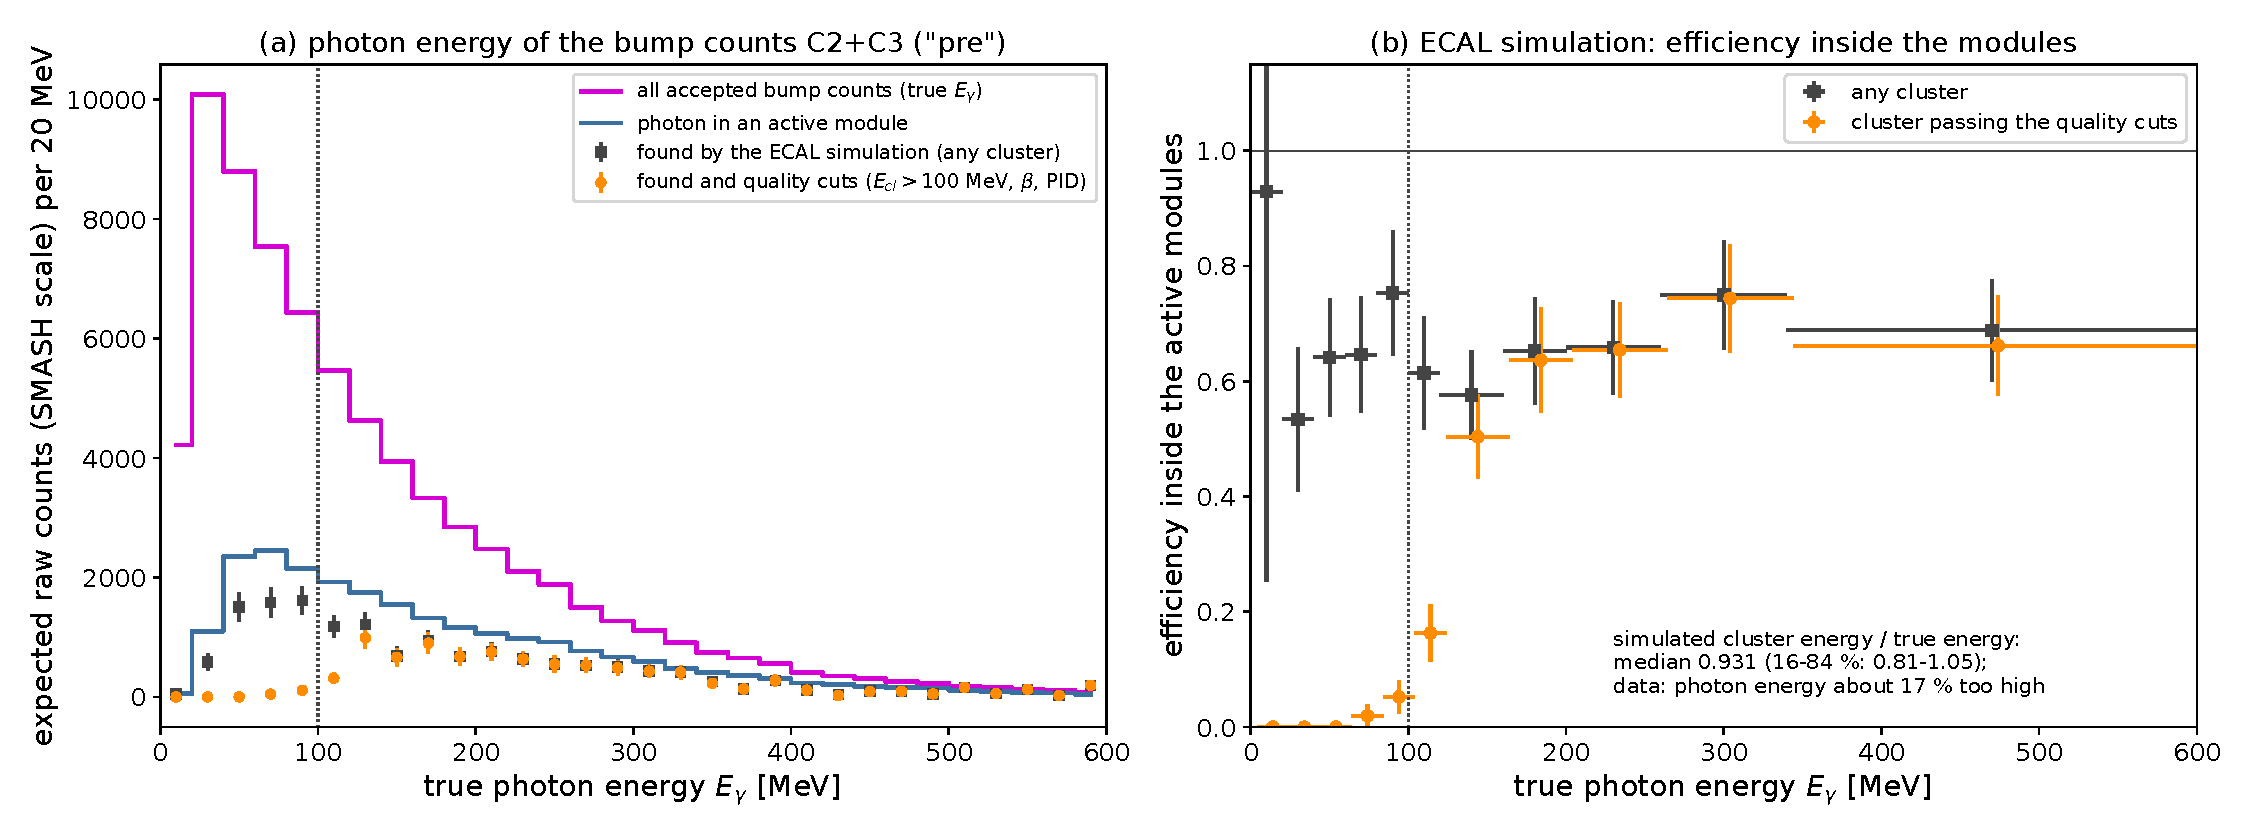
\includegraphics[width=\textwidth]{figs_all/ecalacc_energy_cnt.pdf}
\caption{\textbf{What it shows: half of the lost photons have less than 100\,MeV; inside the modules the simulated ECAL finds
a cluster for about 65\,\% of them at every energy, but the quality cuts remove almost everything below 120\,MeV.} Selection: SMASH simulation only (standard set, which holds the bump counts in mode~A; PDG branching ratios $\times$ the $\eta$-decay physics weights V3); Part~III base selection ``pre'', the same cuts as ``pre'' of this part = simulated PT3 trigger (bit 8192 set), event vertex in the target region ($z>-160$\,mm), \betanew particle identification (pions within $3\sigma$, leptons within $5\sigma$ and with a RICH ring), corrected momenta of all four tracks, all stored combinations of each event (isBest\,$\ge0$); bump classes 2 and 3 at all \Mfour, \Mee and \Mpipi, only counts whose lost photon has a solution on its circle; (a) in expected raw counts at the data luminosity 6079.2\,\nbinv per 20\,MeV of true photon energy; a photon counts as found if a cluster of the true photon lies in an active module; ECAL quality cuts: identified as a photon (PID~1), $0.8<\beta<1.2$, $E_{\mathrm{cluster}}>100$\,MeV. Later
finding of Part~III (file \code{figs_all/ecalacc_energy_cnt.pdf} of \code{report_all.pdf}); simulation only. (a) True photon
energy of the accepted bump counts, classes 2+3 (``pre''): all (magenta) and in an active module (blue), from the photon
reconstructed on its circle; photons found by the ECAL simulation (any cluster: grey; passing the quality cuts PID~1,
$0.8<\beta<1.2$, $E_{\mathrm{cluster}}>100$\,MeV: orange), from the cluster truth. (b) Efficiency inside the active modules
(found / in a module) against the true energy. The text in (b) quotes the simulated energy scale (median
$E_{\mathrm{cluster}}/E_{\mathrm{true}}=0.931$ with the cuts) and the data scale, about 17\,\% high (Part~II).}
\label{fig:s5ecalenergy}
\end{figure}

\notebox{\textbf{Later finding (Part~III, \code{report_all.pdf}, section ``Full reconstruction of the bump with the ECAL
photon''; package ``ecalacc'' and its independent verification): the lost photon of the bump.} In short: one third of
the lost photons of the bump hit an active ECAL module, half of all lost photons are below 100\,MeV, and about one bump
count in ten is fully reconstructed in the simulation.
\begin{itemize}\setlength{\itemsep}{0pt}
\item \textbf{How.} The simulation does not store the lost photon of a bump combination. The four true charged momenta fix it up
      to one angle: with the \ee pair it must give $m_{\piz}$, with all four tracks $m_\eta$, so it lies on a known circle.
      Its position on the circle follows the SMASH $\eta$ spectrum (HGeant decays the $\eta$ by phase space). Every accepted
      count of classes 2 and 3 (``pre'', 2\,836 simulated entries of the standard set, weights $\times$ V3) thus gets the distribution of
      its photon direction and energy, which is tested against the ECAL of \S\ref{sec:ecalsim}. Check: the 598 photons that
      the ECAL simulation did find lie on the predicted circle ($|\Delta\cos|<10^{-3}$ for 99.8\,\%) and 99.5\,\% of them in
      the predicted active modules; the found share is 0.56--0.68 of the predicted probability in every bin, so the
      direction distribution along the circle is right.
\item \textbf{Direction.} Over the whole sphere 9.0\,\% of the lost photons fly below the ECAL band, 54.5\,\% into it and
      36.5\,\% above it (9.9\,\% backward); 68.9\,\% fly into the tracking range 18--85$^\circ$. $32.7\pm0.4$\,\% hit an active
      module (40.3\,\% with six working sectors), the same for classes 2 and 3 and flat in \Mpipi (31.3--33.3\,\%).
\item \textbf{Energy.} The photon is soft: mean true energy 130\,MeV (172\,MeV in the modules), 51\,\% below 100\,MeV
      (34\,\% in the modules); at the edge it takes the smallest possible energy. Only 21.6\,\% of the counts have their
      photon in a module with more than 100\,MeV, 13\,\% near the edge.
\item \textbf{ECAL simulation.} Inside the active modules it finds a cluster of the true photon for 65\,\% of the photons,
      at every energy (not explained; about 4\,\% of the counts have a cluster from an $e^\pm$ of the converted photon
      instead). With the quality cuts (neutral, $0.8<\beta<1.2$, $E_{\mathrm{cluster}}>100$\,MeV) 38\,\% remain: none below
      60\,MeV, 0.16 at 100--120\,MeV, 0.50 at 120--160\,MeV and 0.64--0.75 above. The simulated cluster energy is 7--9\,\% low
      (median $E_{\mathrm{cluster}}/E_{\mathrm{true}}$ 0.914 for all found photons, 0.931 with the cuts, from the cluster
      truth), so the 100\,MeV cut sits near 108\,MeV of true energy (in the data, near 85\,MeV: Part~II). The simulation
      always has a start-detector hit, so the START dependence of the photon $\beta$ cut seen in the data is absent.
\item \textbf{Fully reconstructed} (tagged with the true photon, $m_{5c}$ in 0.49--0.62\,\GeVcc): $9.8\pm0.6$\,\% of the
      bump counts, 14.1\,\% with the cluster energies $\times1.285$ (the scale of the data); 18.6\,\% more than 100\,\MeVcc
      below the edge, 6.9\,\% near it. Of the tagged weight 27.5\,\% lies more than 60\,\MeVcc below the edge (bump:
      16.5\,\%), 46.7\,\% at $-60\ldots-20$\,\MeVcc (44.9\,\%) and 25.8\,\% above $-20$\,\MeVcc (38.2\,\%): the tag weights the
      bump differently from the edge, preferentially far below it. The tag is specific to the bump: 12.7\,\% of the bump counts
      are tagged, 0.8\,\% of class~4 and 1.8\,\% of class~5 (the peak makes about 2.2\,\% of the tagged weight). About
      390 simulated entries of the standard set are tagged, so the simulated tag has an MC error of 9\,\%.
\end{itemize}
\begin{center}\footnotesize
\begin{tabular}{@{}l r r r r r@{}}
\toprule
\% of the accepted bump counts (``pre'') & class 2 & class 3 & 2+3 & 2+3, window B & 2+3, edge \\
\midrule
photon in an active ECAL module & 32.9 & 32.3 & $32.7\pm0.4$ & 31.9 & 31.5 \\
\quad six full sectors & 40.5 & 40.1 & 40.3 & 39.5 & 38.5 \\
\quad and $E_\gamma^{\mathrm{true}}>100$\,MeV & 21.4 & 21.9 & 21.6 & 19.1 & 13.0 \\
found by the ECAL simulation (quality cuts) & 12.3 & 12.6 & $12.4\pm0.7$ & 10.5 & 7.6 \\
fully reconstructed (true photon, $m_{5c}$ window) & 9.9 & 9.6 & $9.8\pm0.6$ & 8.4 & 6.9 \\
\quad cluster energies $\times1.285$ (data-like) & 14.0 & 14.3 & $14.1\pm0.7$ & 13.0 & 11.1 \\
\bottomrule
\end{tabular}\\[2pt]
{\footnotesize Window B: the bump window of Part~III; edge: $-15\ldots+5$\,\MeVcc from the edge $E(\Mpipi,\Mee)$
(\S\ref{sec:s5blind}). Errors: MC (simulation statistics).}
\end{center}}

\emph{Later finding (Part~III, independently verified): the tail of the simulated peak.} The low-side tail of \Mfour in
Table~\ref{tab:s5res} is the leptons' bremsstrahlung in the detector material (HGeant). The generated four-body mass of the
direct decay is a sharp line and the converter has no PHOTOS, so the radiation of the decay itself is missing (leading-log
estimate: about 16--19\,\% more tail counts; result~11, Fig.~\ref{fig:res_peaktail}).


%----------------------------------------------------------------------
\subsection{Cut flow per signal class and background composition}
\label{sec:s5cut}
%----------------------------------------------------------------------
\inshort{inside the windows only the two pion-vertex cuts separate signal from background ($Q$ = 1.04--1.06);
OA$>2^\circ$ is harmful for the $\eta$ ($Q$ = 0.80--0.82) but useful for X17 (1.114); the physical background has the
same make-up (\piz Dalitz and conversion pairs) in every \Mfour region.}
Eight cuts are studied: the four of ``slides'', both pions in the vertex fit,
$\max|z_\pi-z_{\mathrm{vertex}}|<40$\,mm (written $|\Delta z_\pi|$), $\mathrm{MM}_4<2.85$\,\GeVcc and
$p_{T,4}>400$\,\MeVc. For each cut we compute the efficiency $\varepsilon_S$ of the signal and
$\varepsilon_B$ of the background T2 in a window, and
\begin{equation}
Q = \varepsilon_S/\sqrt{\varepsilon_B}.
\end{equation}
$Q$ is the factor by which the cut changes $S/\sqrt{B}$ when $B\gg S$; it needs no luminosity. A cut
carries information if $Q > 1 + \max(0.02, 2\delta Q)$ and is harmful if $Q$ is below the mirror
value. ``Alone'' means the cut on ``pre''; ``N$-$1'' means the cut on top of the other three slides
cuts (for the four other cuts: on top of ``slides''). Errors are from event groups, with pass and
fail counts of one event correlated.

\begin{table}[H]
\centering
\caption{Efficiencies and $Q$ of each cut alone (from ``pre'') in the windows. Peak: $S$ = classes
4+5; bump: $S$ = classes 2+3; X17: $S$ = X17, $B$ = T2 + classes 4+5 (peak window). The error is
in brackets, in units of the last digit.}
\label{tab:s5rank}
\footnotesize
\setlength{\tabcolsep}{3pt}
\begin{tabular}{@{}l ccc ccc cc@{}}
\toprule
 & \multicolumn{3}{c}{peak window} & \multicolumn{3}{c}{bump window} & \multicolumn{2}{c}{X17 (peak window)} \\
cut & $\varepsilon_S$ & $\varepsilon_B$ & $Q$ & $\varepsilon_S$ & $\varepsilon_B$ & $Q$ & $\varepsilon_S$ & $Q$ \\
\midrule
OA$>2^\circ$                     & 0.693(16) & 0.749(8) & 0.801(19) & 0.710(11) & 0.748(7) & 0.820(13) & 0.957 & 1.114(6) \\
$\alpha_{\mathrm{lab}}<50^\circ$ & 0.916(9) & 0.834(7) & 1.003(10) & 0.970(3) & 0.922(4) & 1.010(4) & 0.892 & 0.967(3) \\
$\Mpipi<0.46$                    & 0.981(4) & 0.982(2) & 0.990(4) & 1.000 & 1.000 & 1.000 & 0.980 & 0.989(1) \\
$\alpha_\eta>140^\circ$          & 1.000 & 1.000 & 1.000 & 0.858(10) & 0.947(3) & 0.882(10) & 1.000 & 1.000 \\
pions in vertex fit              & 0.938(7) & 0.806(7) & 1.045(9) & 0.923(6) & 0.784(6) & 1.042(8) & 0.931 & 1.020(4) \\
$|\Delta z_\pi|<40$\,mm          & 0.963(5) & 0.829(7) & 1.058(7) & 0.944(6) & 0.813(6) & 1.047(7) & 0.962 & 1.040(3) \\
$\mathrm{MM}_4<2.85$             & 0.963(5) & 0.904(6) & 1.013(7) & 0.949(5) & 0.886(5) & 1.008(6) & 0.963 & 1.007(3) \\
$p_{T,4}>400$\,\MeVc             & 0.795(12) & 0.588(9) & 1.037(18) & 0.849(8) & 0.712(7) & 1.006(11) & 0.791 & 0.998(6) \\
\midrule
slides (all four), from pre      & 0.606(16) & & 0.790(22) & 0.578(12) & & 0.722(15) & & 1.077(7) \\
\bottomrule
\end{tabular}
\end{table}

What the numbers say (Table~\ref{tab:s5rank}, Figs.~\ref{fig:s5regions} and~\ref{fig:s5rank}):
\begin{itemize}
\item \textbf{Inside the windows the cuts hardly separate signal from the simulated background.}
      Only the two pion-vertex cuts have $Q>1$ significantly ($Q$ = 1.04--1.06 in both windows).
      They select the same counts: given all other cuts, each adds nothing ($Q$ = 0.99--1.02).
      Signal pions come from the primary vertex; 9--15\,\% of the background pion pairs contain a
      $\pi\to\mu$ decay and 28--32\,\% secondary pions.
\item \textbf{OA$>2^\circ$ is harmful for the $\eta$ windows} ($Q = 0.80$ peak, 0.82 bump): it
      removes the signal conversions (classes 3 and 4 keep 0.56--0.57) at the same rate as the
      background conversions. It is informative only for X17 ($Q = 1.114\pm0.006$), whose pairs have a
      median OA of 4.6$^\circ$ against 2.1--2.2$^\circ$ for conversions.
\item \textbf{$\alpha_\eta>140^\circ$} does nothing in the peak window and costs bump signal
      ($Q = 0.882\pm0.010$): it keeps 0.86 of the bump and 0.95 of T2.
\item \textbf{The slides cuts are an \Mfour band-pass} (Fig.~\ref{fig:s5regions}): T2 kept by
      ``slides'' is 0.17 below the bump, 0.64 in the bump window, 0.59 in the peak window, 0.30 in
      0.56--0.70, 0.029 in 0.70--1.00 and $1.8\times10^{-4}$ above 1.00\,\GeVcc. Inside the windows
      they cost 39\,\% (peak) and 42\,\% (bump) of the signal. Their value is a cleaner spectrum
      around the $\eta$ (fits, side bands) and, in data, possibly a smaller CB; neither can be measured
      in this simulation.
\end{itemize}

\begin{figure}[!htbp]
\centering
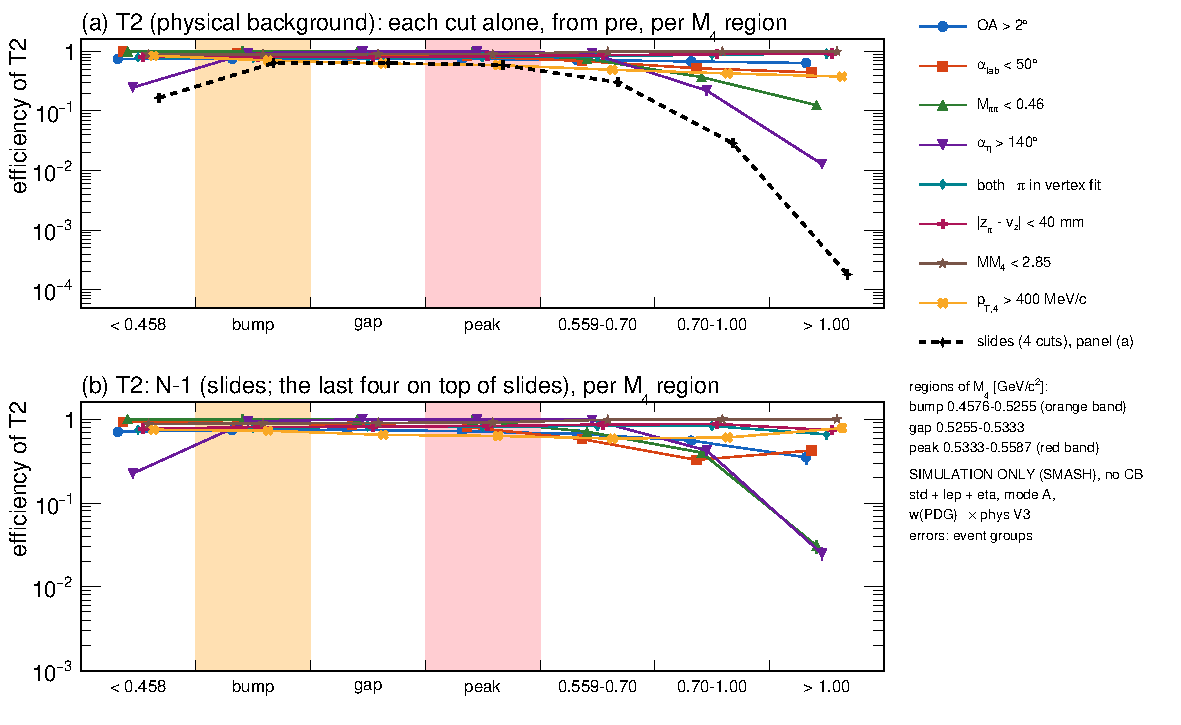
\includegraphics[width=\textwidth]{figs/s5_cut_regions.pdf}
\caption{Efficiency of the physical background T2 per \Mfour region. Selection: SMASH simulation only, no combinatorial background (standard, lepton and $\eta$ sets in mode~A; PDG branching ratios $\times$ the $\eta$-decay physics weights V3); base selection ``pre'' = simulated PT3 trigger (bit 8192 set), event vertex in the target region ($z>-160$\,mm), particle identification by \betanew with the simulation polygons (pions within $3\sigma$, leptons within $5\sigma$ and with a RICH ring), energy-loss-corrected momenta of all four tracks, all stored \ppee combinations per event (isBest\,$\ge0$); only the physical background T2 (a true \ee pair from one decay or conversion with any two pions, no fake lepton); efficiency relative to ``pre'' in (a) and relative to the same selection without the cut in (b); \Mfour regions: below 0.4576, bump window 0.4576--0.5255, gap 0.5255--0.5333, peak window 0.5333--0.5587, 0.5587--0.70, 0.70--1.00 and above 1.00\,\GeVcc (no upper limit); the eight cuts, in the order of the figure: $\mathrm{OA}>2^\circ$ (\ee opening angle), $\alpha_{\mathrm{lab}}<50^\circ$ (angle between the \pipi and \ee momenta in the laboratory), $\Mpipi<0.46$\,\GeVcc, $\alpha_\eta>140^\circ$ (the same angle in the rest frame of a hypothetical $\eta$), these four forming ``slides'', then both pions used in the event-vertex fit, $|\Delta z_\pi|<40$\,mm (both pion tracks within 40\,mm of the event vertex along the beam), $\mathrm{MM}_4<2.85$\,\GeVcc (missing mass of \ppee, computed with $T=4530$\,MeV) and $p_{T,4}>400$\,\MeVc (transverse momentum of \ppee). (a) Each cut alone on
``pre'', and the four slides cuts together (dashed). (b) N$-$1: each cut on top of the other
slides cuts (the last four cuts on top of ``slides''). Errors from event groups.}
\label{fig:s5regions}
\end{figure}

\begin{figure}[!htbp]
\centering
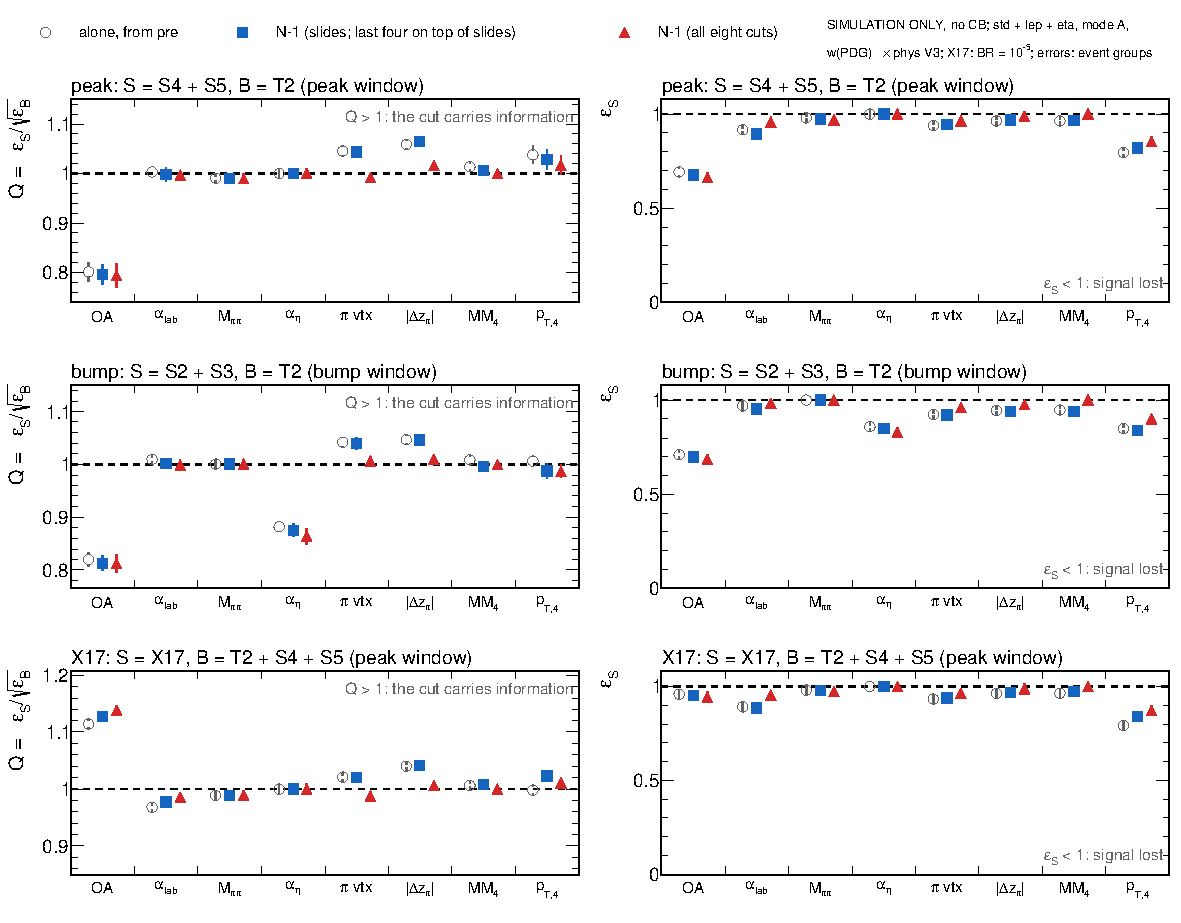
\includegraphics[width=\textwidth]{figs/s5_cut_rank.pdf}
\caption{$Q = \varepsilon_S/\sqrt{\varepsilon_B}$ (left) and $\varepsilon_S$ (right) of the eight cuts
for the peak, the bump and X17 ($\mathrm{BR}=10^{-5}$): alone (open circles), N$-$1 with respect
to ``slides'' (squares), N$-$1 with respect to all eight cuts (triangles). Selection: SMASH simulation only, no combinatorial background (standard, lepton and $\eta$ sets in mode~A; PDG branching ratios $\times$ the $\eta$-decay physics weights V3); base selection ``pre'' = simulated PT3 trigger (bit 8192 set), event vertex in the target region ($z>-160$\,mm), particle identification by \betanew with the simulation polygons (pions within $3\sigma$, leptons within $5\sigma$ and with a RICH ring), energy-loss-corrected momenta of all four tracks, all stored \ppee combinations per event (isBest\,$\ge0$); peak: signal classes 4+5 against T2 in the peak window $0.5333\le\Mfour<0.5587$\,\GeVcc; bump: classes 2+3 against T2 in the bump window $0.4576\le\Mfour<0.5255$\,\GeVcc; X17: X17 counts against T2 plus classes 4+5 in the peak window (in the panel titles S2--S5 are the signal classes 2--5); efficiencies relative to ``pre'' (alone), to ``pre'' plus the other cuts of ``slides'' (squares; the last four cuts on top of all of ``slides'') or to ``pre'' plus the other seven cuts (triangles); the eight cuts, in the order of the figure: $\mathrm{OA}>2^\circ$ (\ee opening angle), $\alpha_{\mathrm{lab}}<50^\circ$ (angle between the \pipi and \ee momenta in the laboratory), $\Mpipi<0.46$\,\GeVcc, $\alpha_\eta>140^\circ$ (the same angle in the rest frame of a hypothetical $\eta$), these four forming ``slides'', then both pions used in the event-vertex fit, $|\Delta z_\pi|<40$\,mm (both pion tracks within 40\,mm of the event vertex along the beam), $\mathrm{MM}_4<2.85$\,\GeVcc (missing mass of \ppee, computed with $T=4530$\,MeV) and $p_{T,4}>400$\,\MeVc (transverse momentum of \ppee).}
\label{fig:s5rank}
\end{figure}

\textbf{Background composition} (Table~\ref{tab:s5comp}). The physical background has the same
make-up in every \Mfour region: \piz Dalitz pairs (L1, 53--60\,\% of T2) and conversion pairs (L3,
28--39\,\%). The pions are mostly both primary (P7, 40--72\,\%) or mixed/secondary (P8, 13--33\,\%);
9--15\,\% of the pion pairs contain a $\pi\to\mu$ decay (P1). $G_\eta$ is 7--10\,\% of T2 around the
$\eta$ and $G_{\mathrm{vec}}$ is negligible. T3 (not in the sum) is 12--20\,\% of T1+T2 near the
$\eta$; 60\,\% of T3 in the peak window are conversion pairs.

\begin{table}[H]
\centering
\caption{Composition after ``pre'' per \Mfour region: $\sigma$ of T1+T2, share of the signal
classes in T1+T2, shares of the groups in T2, and T3, T4 relative to T1+T2 (not in the sum).}
\label{tab:s5comp}
\small
\begin{tabular}{@{}l r r rrr rr@{}}
\toprule
region [\GeVcc] & T1+T2 [nb] & signal share & $G_\eta$ & $G_{\pi^0\mathrm{D}}$ & $G_{\mathrm{conv}}$ & T3 & T4 \\
\midrule
$<0.4576$    & $7.66\pm0.17$ & 0.310(11) & 0.067 & 0.539 & 0.384 & 0.147 & 0.012 \\
bump         & $24.48\pm0.33$ & 0.401(7) & 0.082 & 0.539 & 0.365 & 0.119 & 0.019 \\
gap          & $2.67\pm0.09$ & 0.100(10) & 0.078 & 0.535 & 0.369 & 0.202 & 0.028 \\
peak         & $11.45\pm0.18$ & 0.201(6) & 0.093 & 0.527 & 0.364 & 0.150 & 0.025 \\
0.5587--0.70 & $109.0\pm0.6$ & 0.0013(2) & 0.064 & 0.554 & 0.377 & 0.186 & 0.024 \\
0.70--1.00   & $340.9\pm1.0$ & $<10^{-4}$ & 0.033 & 0.573 & 0.392 & 0.179 & 0.018 \\
$>1.00$      & $205.0\pm0.7$ & 0 & 0.017 & 0.595 & 0.387 & 0.183 & 0.014 \\
\bottomrule
\end{tabular}
\end{table}

\textbf{Statistics.} The std-set signal classes limit every number of this part. In the windows
after ``pre'' class~2 has $N_{\mathrm{eff}} = 1022$, class~3 718 and class~4 225; after all eight
cuts 526, 268 and 79. $G_{\mathrm{vec}}$ and $G_{\mathrm{diff}}$ have $N_{\mathrm{eff}}$ below 150.

%----------------------------------------------------------------------
\subsection{Optimisation for the \texorpdfstring{$\eta$}{eta} peak and bump}
\label{sec:s5opt}
%----------------------------------------------------------------------
\inshort{frozen PEAK = ``pre'' + $|\Delta z_\pi|<40$\,mm + $\mathrm{MM}_4<2.85$\,\GeVcc, DIRECT = ``pre'' +
$|\Delta z_\pi|<40$\,mm, BUMP = ``pre''; gains over ``pre'' $+2.67\pm0.44$ (5.1\,\%) and $+1.12\pm0.10$ (4.0\,\%) in
$F$; the optimisation bias of the freeze rule is below 1\,\%.}
\textbf{Targets.} PEAK: classes 4+5 in the peak window. DIRECT: class 5 in the peak window, with
class~4 counted as background. BUMP: classes 2+3 in the bump window. $B$ = all other T1+T2 counts of
the window; a variant adds T3 and T4.

\textbf{Figure of merit and method.} $F = S/\sqrt{S+B}$ with $S$, $B$ in expected counts at
$\Ldata$ (UNCONFIRMED; $F\propto\sqrt{\Ldata}$, the position of the optimum does not depend on it).
Nine cut variables are scanned on grids that contain every named selection: OA$>$ (10 values),
$\alpha_{\mathrm{lab}}<$ (10), $\Mpipi>$ (9), $\Mpipi<$ (10), $\alpha_\eta>$ (8), pions in the
vertex fit (off/on), $|\Delta z_\pi|<40$\,mm (off/on), $\mathrm{MM}_4<$ (8) and $p_{T,4}>$ (6),
$13\,824\,000$ combinations in all. Each entry of the window gets a grid index per variable; the weights are
filled into a 9-dimensional histogram and summed cumulatively along every axis. After that each
cell holds the exact $S$ and $B$ of one combination, and every cell is evaluated (exhaustive
search, no random sampling). The table reproduces the engine sums for all named selections and
direct loops over the entries for 30 random cells (relative difference $<10^{-9}$; 378 checks).

\textbf{Freeze rule} (declared before the search). A candidate must reach $F\ge0.95\,F_{\mathrm{best}}$ on
the full sample and on each half (relative to the best of that half). Among the candidates take
the one with the fewest active cuts, then the one whose worst grid neighbour (each active
threshold moved by one step) has the highest $F$.

\begin{table}[H]
\centering
\caption{Optimisation of the $\eta$ selection (full sample, $\Ldata = 6080.5\,\nbinv$
UNCONFIRMED; errors: simulation statistics). $|\Delta z_\pi|$ stands for $\max|z_\pi-z_{\mathrm{vertex}}|<40$\,mm.
The last two rows are differences of $F$ with the event-group error computed on the difference
itself: the same counts enter both selections, so this error is much smaller than the errors of the
two $F$.}
\label{tab:s5opt}
\small
\begin{tabularx}{\textwidth}{@{}>{\raggedright\arraybackslash}p{3.6cm} L L L@{}}
\toprule
 & PEAK & DIRECT & BUMP \\
\midrule
$F$ at ``pre'' (purity) & $52.12\pm1.51$ (0.198) & $27.83\pm0.23$ (0.105) & $152.7\pm3.0$ (0.396) \\
best cell & $\Mpipi$ 0.32--0.48, $\alpha_\eta>160^\circ$, $|\Delta z_\pi|$, $\mathrm{MM}_4<2.85$
          & $\Mpipi$ 0.30--0.53, $\alpha_\eta>150^\circ$, $|\Delta z_\pi|$, $\mathrm{MM}_4<2.85$
          & $\alpha_{\mathrm{lab}}<70^\circ$, $\Mpipi$ 0.30--0.41, $|\Delta z_\pi|$ \\
$F$ of the best cell (purity) & $56.18\pm1.74$ (0.262) & $29.50\pm0.28$ (0.130) & $157.0\pm3.2$ (0.467) \\
frozen cut & $|\Delta z_\pi|<40$\,mm, $\mathrm{MM}_4<2.85$ & $|\Delta z_\pi|<40$\,mm & none (= pre) \\
$F$ frozen ($F/F_{\mathrm{best}}$) & $54.79\pm1.63$ (0.975) & $28.95\pm0.26$ (0.982) & $152.7\pm3.0$ (0.973) \\
purity, efficiency (frozen) & $0.234\pm0.007$, $0.931\pm0.007$ & $0.119\pm0.002$, $0.963\pm0.001$ & $0.396\pm0.007$, 1 \\
$F$(frozen) $-$ $F$(pre) & $+2.67\pm0.44$ & $+1.12\pm0.10$ & 0 \\
$F$(frozen) $-$ $F$(pre + pions in vertex fit) & $+1.19\pm0.48$ & $+0.58\pm0.09$ & $-1.11\pm0.88$ \\
\bottomrule
\end{tabularx}
\end{table}

\textbf{Results} (Table~\ref{tab:s5opt}, Figs.~\ref{fig:s5profile} and~\ref{fig:s5optcomp}).
\begin{itemize}
\item \textbf{The surface of $F$ is flat.} The plateau ($F\ge0.95\,F_{\mathrm{best}}$) contains, for PEAK:
      OA none or $>1^\circ$; $\alpha_{\mathrm{lab}}<40^\circ$ or looser; $\Mpipi>$ none to 0.34;
      $\Mpipi<0.46$ or looser; any $\alpha_\eta$ up to 170$^\circ$; $\mathrm{MM}_4<2.7$ or looser;
      $p_{T,4}>400$ or looser. The other targets are similar.
\item \textbf{The frozen cuts are better than ``pre'', but only a little.} With the correlated
      error the gain is significant in the simulation: $+2.67\pm0.44$ (5.1\,\%) for PEAK and
      $+1.12\pm0.10$ (4.0\,\%) for DIRECT. Compared with ``pre + pions in vertex fit'' the frozen
      cuts gain $+1.19\pm0.48$ (PEAK) and $+0.58\pm0.09$ (DIRECT). For BUMP no cut is frozen; the
      best cell gains $+4.3\pm1.0$, but this includes the optimisation bias (below).
\item \textbf{The PEAK choice was a knife edge.} ``$|\Delta z_\pi|<40$\,mm'' alone reaches 0.966 of
      $F_{\mathrm{best}}$ on the full sample but 0.9494 on half~B: it missed the half condition by
      0.0006, and the rule added $\mathrm{MM}_4<2.85$ (+1\,\% in $F$). On random halves the rule picks
      ``$|\Delta z_\pi|<40$\,mm'' alone in 167 of 200 cases.
\item \textbf{OA$>2^\circ$ is off the plateau for all three targets}, even for DIRECT, where it keeps
      only 0.81 of the direct decay. Only ``pions in vertex fit'', ``peak nominal'' and (for BUMP)
      ``bump nominal'' are on the plateau (Table~\ref{tab:s5presets}).
\item \textbf{Purity.} The cuts can raise the purity at a small loss of $F$: for BUMP, ``bump
      nominal'' gives 0.456 and the best purity on the plateau ($\alpha_{\mathrm{lab}}<40^\circ$,
      $\Mpipi>0.32$, $|\Delta z_\pi|$) 0.496, against 0.396 at ``pre''. These purity choices are not
      stable between halves (the most frequent half pick occurs in only 32--61 of 200 cases).
\end{itemize}

\begin{table}[H]
\centering
\caption{Named selections: $F/F_{\mathrm{best}}$ per target (errors about 3\,\% PEAK, 1\,\% DIRECT,
2\,\% BUMP; $\Ldata$ UNCONFIRMED).}
\label{tab:s5presets}
\small
\begin{tabular}{@{}l ccc@{}}
\toprule
selection & PEAK & DIRECT & BUMP \\
\midrule
pre                     & 0.928 & 0.943 & 0.973 \\
pre + OA$>2^\circ$       & 0.748 & 0.889 & 0.806 \\
pre + pions in vertex fit & 0.954 & 0.962 & 0.980 \\
slides                  & 0.730 & 0.889 & 0.716 \\
old code                & 0.784 & 0.848 & 0.877 \\
peak nominal            & 0.941 & 0.953 & 0.979 \\
bump nominal            & 0.732 & 0.783 & 0.977 \\
\bottomrule
\end{tabular}
\end{table}

\begin{figure}[!htbp]
\centering
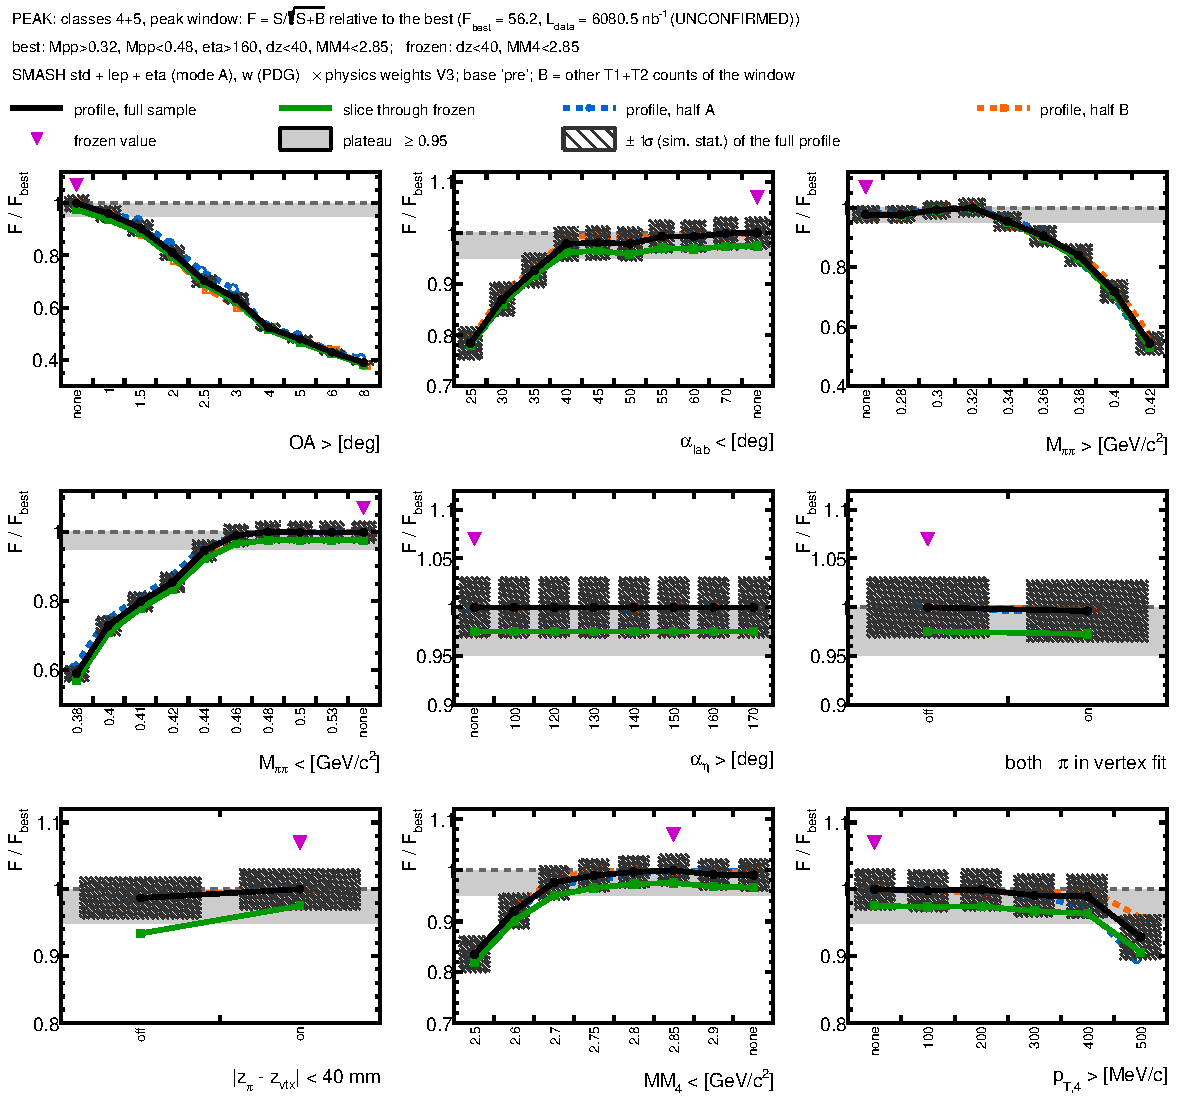
\includegraphics[width=\textwidth]{figs/s5_opt_eta_profile_peak_cnt.pdf}
\caption{PEAK target: $F/F_{\mathrm{best}}$ against each cut variable. Selection: SMASH simulation only, no combinatorial background (standard, lepton and $\eta$ sets in mode~A; PDG branching ratios $\times$ the $\eta$-decay physics weights V3); base selection ``pre'' = simulated PT3 trigger (bit 8192 set), event vertex in the target region ($z>-160$\,mm), particle identification by \betanew with the simulation polygons (pions within $3\sigma$, leptons within $5\sigma$ and with a RICH ring), energy-loss-corrected momenta of all four tracks, all stored \ppee combinations per event (isBest\,$\ge0$); on top of ``pre'' the nine scanned cuts: \ee opening angle above none or 1--$8^\circ$, angle between the \pipi and \ee momenta in the laboratory below 25--$70^\circ$ or none, \Mpipi above none or 0.28--0.42\,\GeVcc and below 0.38--0.53\,\GeVcc or none, the same angle in the rest frame of a hypothetical $\eta$ above none or 100--$170^\circ$, both pions used in the event-vertex fit off or on, both pion tracks within 40\,mm of the event vertex along the beam off or on, missing mass of \ppee below 2.5--2.9\,\GeVcc or none (computed with $T=4530$\,MeV), transverse momentum of \ppee above none or 100--500\,\MeVc; signal $S$ = classes 4+5 and background $B$ = all other T1+T2 counts of the peak window $0.5333\le\Mfour<0.5587$\,\GeVcc, in expected counts at \Ldata; frozen point (PEAK): the 40\,mm pion cut and $\mathrm{MM}_4<2.85$\,\GeVcc, no other cut; halves A and B = even and odd event groups, each weighted $\times2$. Profile = the best $F$ over
all other variables at a fixed value (full sample, black; half A and half B relative to their
own best, dashed). The hatched band is the $\pm1\sigma$ statistical error of the full-sample $F$
at each profile point; differences between neighbouring points are much more precise, because
the counts are shared. Green: slice through the frozen point. Grey band: plateau
($\ge0.95$). Triangle: frozen value. $\Ldata = 6080.5\,\nbinv$ (UNCONFIRMED).}
\label{fig:s5profile}
\end{figure}

\begin{figure}[!htbp]
\centering
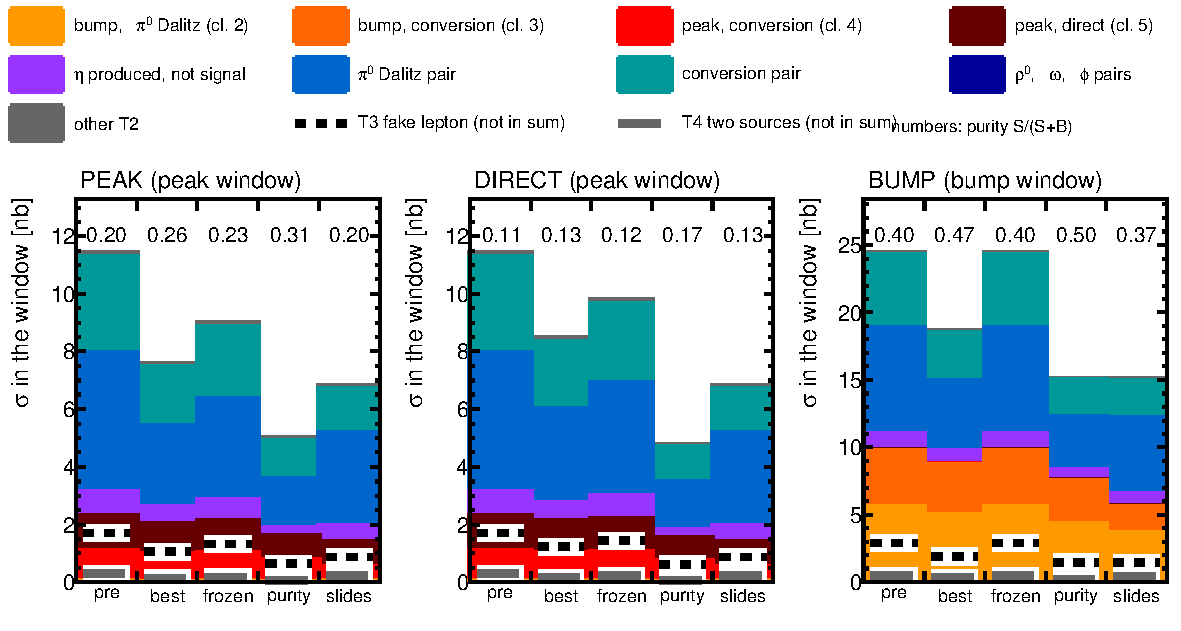
\includegraphics[width=\textwidth]{figs/s5_opt_eta_composition.pdf}
\caption{Content of the target window by group, $\sigma$ in nb, for ``pre'', the best cell, the
frozen cut, the best purity on the plateau and ``slides'' (stacked: T1+T2 groups). Selection: SMASH simulation only, no combinatorial background (standard, lepton and $\eta$ sets in mode~A; PDG branching ratios $\times$ the $\eta$-decay physics weights V3); base selection ``pre'' = simulated PT3 trigger (bit 8192 set), event vertex in the target region ($z>-160$\,mm), particle identification by \betanew with the simulation polygons (pions within $3\sigma$, leptons within $5\sigma$ and with a RICH ring), energy-loss-corrected momenta of all four tracks, all stored \ppee combinations per event (isBest\,$\ge0$); panels: PEAK (signal classes 4+5) and DIRECT (signal class~5, class~4 counted as background) in the peak window $0.5333\le\Mfour<0.5587$\,\GeVcc, BUMP (classes 2+3) in the bump window $0.4576\le\Mfour<0.5255$\,\GeVcc; the five bars, all on top of ``pre'': ``pre'' alone; the best cell (PEAK: $0.32<\Mpipi<0.48$\,\GeVcc, $\alpha_\eta>160^\circ$, $\Delta z_\pi<40$\,mm, $\mathrm{MM}_4<2.85$\,\GeVcc; DIRECT: $0.30<\Mpipi<0.53$\,\GeVcc, $\alpha_\eta>150^\circ$, $\Delta z_\pi<40$\,mm, $\mathrm{MM}_4<2.85$\,\GeVcc; BUMP: $\alpha_{\mathrm{lab}}<70^\circ$, $0.30<\Mpipi<0.41$\,\GeVcc, $\Delta z_\pi<40$\,mm); the frozen cut (PEAK: $\Delta z_\pi<40$\,mm and $\mathrm{MM}_4<2.85$\,\GeVcc; DIRECT: $\Delta z_\pi<40$\,mm; BUMP: none); the best purity on the plateau (PEAK: $\Mpipi>0.32$\,\GeVcc, $\Delta z_\pi<40$\,mm, $\mathrm{MM}_4<2.7$\,\GeVcc; DIRECT: $\alpha_{\mathrm{lab}}<40^\circ$, $\Delta z_\pi<40$\,mm, $\mathrm{MM}_4<2.7$\,\GeVcc; BUMP: $\alpha_{\mathrm{lab}}<40^\circ$, $\Mpipi>0.32$\,\GeVcc, $\Delta z_\pi<40$\,mm); ``slides'' ($\mathrm{OA}>2^\circ$, $\alpha_{\mathrm{lab}}<50^\circ$, $\Mpipi<0.46$\,\GeVcc, $\alpha_\eta>140^\circ$). OA is the \ee opening angle, $\alpha_{\mathrm{lab}}$ the angle between the \pipi and \ee momenta in the laboratory, $\alpha_\eta$ the same angle in the rest frame of a hypothetical $\eta$, $\Delta z_\pi$ the larger distance of the two pion tracks from the event vertex along the beam and $\mathrm{MM}_4$ the missing mass of \ppee (computed with $T=4530$\,MeV). T3 (dashed
line) and T4 (dash-dotted line) are drawn at their own level and are not in the stack. Numbers
above the bars: purity $S/(S+B)$.}
\label{fig:s5optcomp}
\end{figure}

\textbf{Split-half check of the optimisation bias.} The entries are split by event group into two
halves (half A = even group number, half B = odd; each half weighted by 2). The search is run on
one half and the chosen cell is evaluated on the other. The bias is $F$(optimising half) $-$
$F$(other half), averaged over both directions, because a single direction also contains the
difference between the halves at fixed cuts (PEAK at ``pre'': $F_A = 51.28$, $F_B = 52.97$).
\begin{center}
\small
\begin{tabular}{@{}l ccc ccc@{}}
\toprule
 & \multicolumn{3}{c}{100 random splits (mean $\pm$ error of the mean)} & \multicolumn{3}{c}{deterministic split (A/B)} \\
target & best cell & freeze rule & purity rule & best cell & freeze rule & purity rule \\
\midrule
PEAK   & $+2.71\pm0.11$\,\% & $+0.68\pm0.09$\,\% & $+1.55\pm0.15$\,\% & $+2.08$\,\% & $+1.77$\,\% & $+0.61$\,\% \\
DIRECT & $+0.75\pm0.05$\,\% & $+0.06\pm0.01$\,\% & $+0.80\pm0.07$\,\% & $+0.37$\,\% & 0.00\,\% & $+1.65$\,\% \\
BUMP   & $+1.10\pm0.07$\,\% & $+0.08\pm0.01$\,\% & $+1.64\pm0.09$\,\% & $+0.65$\,\% & 0.00\,\% & $+1.30$\,\% \\
\bottomrule
\end{tabular}
\end{center}
The gain of the best cell over ``pre'' (PEAK $+7.8$\,\%, DIRECT $+6.0$\,\%, BUMP $+2.8$\,\%) is partly
this bias; the freeze rule reduces it to below 1\,\%. Single directions range from $-7.7$ to
$+9.2$\,\%: this is the noise between halves, set by the std set. The limiting components are
class~4 ($N_{\mathrm{eff}}$ 209 at the frozen PEAK cut; it gives almost all of the 3.0\,\% error of $F$),
the std part of $B$ ($N_{\mathrm{eff}}$ 924) and, for BUMP, the signal itself ($N_{\mathrm{eff}}$ 1739).

\notebox{\textbf{Frozen $\eta$ selections} (\code{plots/eta_sim/}\allowbreak\code{tables/s5_opt_eta_frozen.txt}):
PEAK = pre + $|\Delta z_\pi|<40$\,mm + $\mathrm{MM}_4<2.85$\,\GeVcc; DIRECT = pre + $|\Delta z_\pi|<40$\,mm;
BUMP = pre. \textbf{Caveat for data:} $|\Delta z_\pi|$ needs the $z$ of the pion tracks, which the
compact data entries (\code{ScanEngine.h}) do not have yet. The data-ready alternative on the plateau is
``pre + pions in vertex fit'' ($F/F_{\mathrm{best}}$ = 0.954, 0.962, 0.980). Without CB the
simulation-only optimum may be looser than the data optimum, since the CB and its subtraction
add to the variance and the cuts also reduce the CB.}

%----------------------------------------------------------------------
\subsection{A selection aimed at X17 and its expected limit}
\label{sec:s5x17}
%----------------------------------------------------------------------
\inshort{the frozen X17 selection (peak window, $15.5\le\Mee<24.5$\,\MeVcc, both pions in the vertex fit) gives an
expected 90\,\% CL limit of $1.9\times10^{-5}$ (preliminary; phase-space and isotropic X17 assumed), set by the
simulation error of the background; $5.7\times10^{-6}$ if the background were known exactly.}
\textbf{The X17 line.} In the peak window after ``pre'', the reconstructed \Mee of the X17 counts has
a mean of $17.25\pm0.01$\,\MeVcc and a Gaussian core of $\sigma = 4.04\pm0.01$\,\MeVcc; 93.3\,\% lie
within $\pm2\sigma$. The width depends on the opening angle: 4.5\,\MeVcc for OA$<2^\circ$,
3.3\,\MeVcc for OA$>8^\circ$; the mean moves from 13.6 (OA$<3^\circ$) to 20.3\,\MeVcc
(OA$>8^\circ$), so an OA cut reshapes the line. In \Mfour the X17 counts have mean 546.6\,\MeVcc and
$\sigma = 5.9$\,\MeVcc; 85.7\,\% of them lie in the peak window.

\textbf{Figure of merit.} The expected 90\,\% CL upper limit on
$\mathrm{BR}\equiv\mathrm{BR}(\eta\to\pipi X17)\,\mathrm{BR}(X17\to\ee)$ from counting in a window,
for $\mathrm{BR}=0$:
\begin{equation}
\mathrm{UL} = \sqrt{\mathrm{UL}_{\mathrm{stat}}^2 + \left(1.645\,\sigma_{B,\mathrm{MC}}/s_1\right)^2},
\qquad \mathrm{UL}_{\mathrm{stat}} = s_{\mathrm{up}}(B)/s_1 .
\label{eq:s5ul}
\end{equation}
Here $s_1$ is the number of selected X17 counts per unit BR and $B$ the background counts (T1 without
X17, plus T2), both at \Ldata; $s_{\mathrm{up}}(B)$ is the CLs upper limit on the signal for an
observed count equal to $B$ (continuous Poisson, about $1.645\sqrt{B}$ for large $B$); and
$\sigma_{B,\mathrm{MC}}$ is the simulation (event-group) error of $B$. The second term is there
because a counting analysis takes $B$ from this simulation. $\mathrm{UL}_{\mathrm{stat}}$ alone is
the limit with the background known exactly: a statistical limit only.

\textbf{Two versions.} The first optimisation (v1, used by the blind test of
Sect.~\ref{sec:s5blind}) used $\mathrm{UL}_{\mathrm{stat}}$ and also optimised the edges of the
\Mfour window. A review found two problems: the MC error of $B$ ($\pm307$ counts) is larger than
the statistical term, and the \Mfour window was to stay fixed for all parts of the study. The
optimisation was therefore repeated (v2) with Eq.~(\ref{eq:s5ul}) and the fixed peak window.
Method: coordinate descent over \Mee window, OA (lower and upper), $\alpha_{\mathrm{lab}}$,
\Mpipi (lower and upper), $\alpha_\eta$ and pions in the vertex fit; in each step the loosest value
within 2\,\% of the step minimum is taken. Two different starting points end at the same optimum.

\begin{table}[H]
\centering
\caption{X17 selections after ``pre''. Counts at $\Ldata = 6080.5\,\nbinv$ (UNCONFIRMED). UL in
units of $10^{-6}$; ``shape'': binned likelihood of \Mee 2--62\,\MeVcc in the \Mfour window with a
Gaussian X17 line (background shape from the simulation, normalisation known or free).
$Z$: Asimov significance for $\mathrm{BR}=10^{-5}$ with $B$ known.}
\label{tab:s5x17}
\small
\begin{tabularx}{\textwidth}{@{}L >{\raggedright\arraybackslash}p{4.4cm} >{\raggedright\arraybackslash}p{4.4cm}@{}}
\toprule
 & v1 (blind test) & v2 (frozen) \\
\midrule
cuts in addition to ``pre'' & \Mfour 0.5330--0.5555, \Mee 13.0--26.5, pions in vertex fit
                            & \Mfour 0.5333--0.5587, \Mee 15.5--24.5, pions in vertex fit \\
X17 counts per unit BR, $s_1$  & $2.727\times10^{7}$ & $2.127\times10^{7}$ \\
X17 counts at $\mathrm{BR}=10^{-5}$ & 272.7 & 212.7 \\
background $B$ [nb] ($N_{\mathrm{eff}}$) & $1.333\pm0.051$ (696) & $0.878\pm0.039$ (501) \\
background counts $B\pm\sigma_{B,\mathrm{MC}}$ & $8108\pm307$ & $5342\pm239$ \\
$\mathrm{UL}_{\mathrm{stat}}$ (B known exactly) & 5.48 & 5.71 \\
$\mathrm{UL}$, Eq.~(\ref{eq:s5ul}) (with the MC error of $B$) & 19.3 & 19.3 \\
shape, $B$ known / normalisation free & 4.85 / 5.40 & 4.96 / 5.54 \\
$Z$($\mathrm{BR}=10^{-5}$), $B$ known / with $\sigma_{B,\mathrm{MC}}$ & 3.01 / 0.85 & 2.89 / 0.85 \\
\bottomrule
\end{tabularx}
\end{table}

\textbf{Results} (Table~\ref{tab:s5x17}, Fig.~\ref{fig:s5x17shape}).
\begin{itemize}
\item \textbf{The MC error of the background sets the limit.} With the MC term the expected limit is
      $1.93\times10^{-5}$ for both selections, 3.4--3.5 times $\mathrm{UL}_{\mathrm{stat}}$. The
      re-optimisation gains nothing: the v1 cuts give $1.933\times10^{-5}$, the v2 cuts
      $1.931\times10^{-5}$. ``slides'' with the same \Mee window gives $2.15\times10^{-5}$.
\item \textbf{Where the MC error comes from.} At the v2 optimum the variance of $B$ comes from
      $G_{\pi^0\mathrm{D}}$ (60\,\%; lep set, $N_{\mathrm{eff}}$ 313), $G_{\mathrm{conv}}$ (24\,\%; 19 standard-set
      entries, $N_{\mathrm{eff}}$ 18) and $G_\eta$ (12\,\%; $N_{\mathrm{eff}}$ 29). One standard-set entry stands for 27.5
      expected data counts.
\item \textbf{Cuts.} The \Mee window keeps 0.62 of X17 and 0.094 of $B$; the pion-vertex cut keeps
      0.93 of X17 and 0.82 of $B$. OA, $\alpha_{\mathrm{lab}}$, \Mpipi and $\alpha_\eta$ cuts do not
      lower the limit: at \Mee 12--22\,\MeVcc the OA medians of X17 (4.9$^\circ$), the direct decay
      (4.6$^\circ$) and $G_{\pi^0\mathrm{D}}$ (5.2$^\circ$) are about the same. Later confirmed by Part~III (note below).
\item \textbf{Composition of $B$} (v1): $G_{\pi^0\mathrm{D}}$ 0.56, direct decay (class 5) 0.18,
      $G_{\mathrm{conv}}$ 0.12, $G_\eta$ 0.08, class 4 0.03. The direct decay is an irreducible
      background under the line.
\item \textbf{Split halves} (v2 figure of merit): the optimum of half A gives 28.1 on A and 30.2 on
      B, that of half B 24.4 and 28.1 (in $10^{-6}$; each half has a $\sqrt2$ larger MC error). The
      bias is 7--15\,\%: with the MC term the figure of merit is itself noisy, and the optimum
      (\Mee 13--27.5 on half A, 15.5--23.5 on half B) is not better determined than in v1.
\end{itemize}

\begin{figure}[!htbp]
\centering
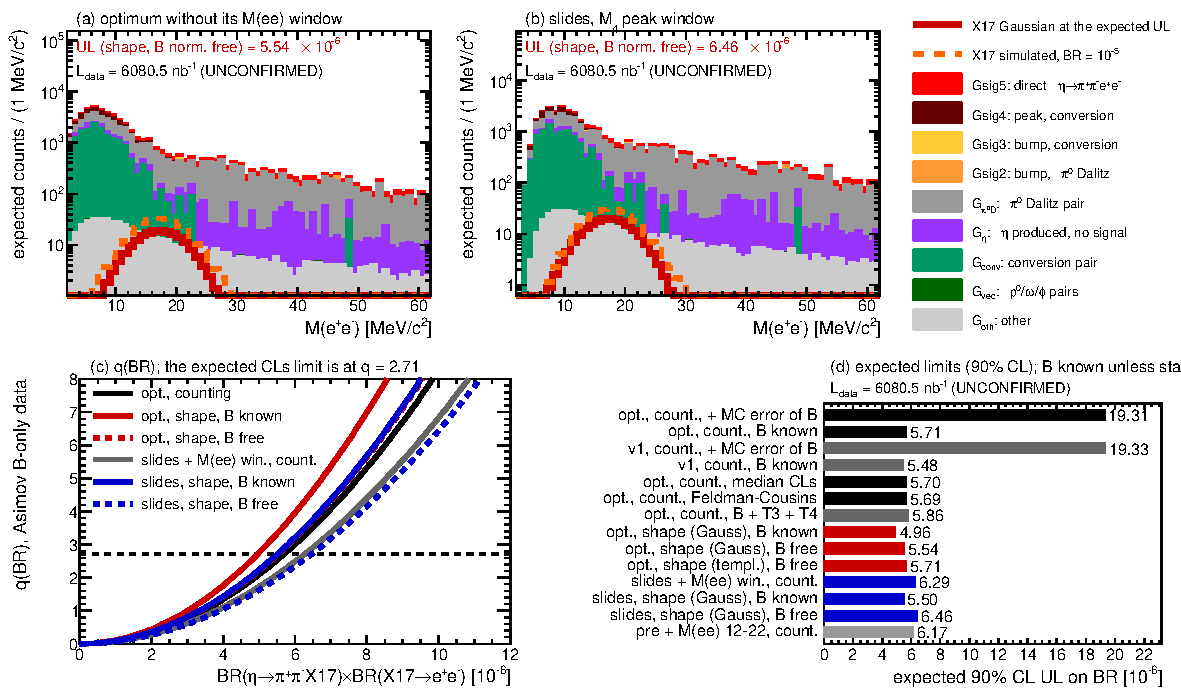
\includegraphics[width=\textwidth]{figs/s5_opt_x17_shape_cnt.pdf}
\caption{X17 search, expected counts at $\Ldata = 6080.5\,\nbinv$ (UNCONFIRMED). Selection: SMASH simulation only, no combinatorial background (standard, lepton and $\eta$ sets in mode~A; PDG branching ratios $\times$ the $\eta$-decay physics weights V3); base selection ``pre'' = simulated PT3 trigger (bit 8192 set), event vertex in the target region ($z>-160$\,mm), particle identification by \betanew with the simulation polygons (pions within $3\sigma$, leptons within $5\sigma$ and with a RICH ring), energy-loss-corrected momenta of all four tracks, all stored \ppee combinations per event (isBest\,$\ge0$); all panels inside the peak window $0.5333\le\Mfour<0.5587$\,\GeVcc; (a) the frozen X17 selection v2 without its \Mee window: ``pre'' plus both pions used in the event-vertex fit, \Mee 2--62\,\MeVcc in 1\,\MeVcc bins (the frozen window $15.5\le\Mee<24.5$\,\MeVcc is not applied); (b) ``pre'' plus the four ``slides'' cuts instead of the pion-vertex cut: $\mathrm{OA}>2^\circ$ (\ee opening angle), $\alpha_{\mathrm{lab}}<50^\circ$ (angle between the \pipi and \ee momenta in the laboratory), $\Mpipi<0.46$\,\GeVcc and $\alpha_\eta>140^\circ$ (the same angle in the rest frame of a hypothetical $\eta$); \Mee 2--62\,\MeVcc; (c) and (d): the shape fits use \Mee 2--62\,\MeVcc, the counting limits $15.5\le\Mee<24.5$\,\MeVcc; ``opt.'' = v2, ``v1'' = $0.5330\le\Mfour<0.5555$\,\GeVcc, $13.0\le\Mee<26.5$\,\MeVcc and pions in the vertex fit, ``pre + M(ee) 12--22'' = peak window and $12\le\Mee<22$\,\MeVcc only; background $B$ = T1 without X17 plus T2 (one entry adds T3 and T4). (a) \Mee at the v2
optimum without its \Mee window, stacked background groups, X17 as a Gaussian at the expected limit
of the shape fit and as the simulated template at $\mathrm{BR}=10^{-5}$. (b) The same for
``slides''. (c) Test statistic $q(\mathrm{BR})$ on Asimov background-only data; the expected
CLs limit is at $q = 2.71$. (d) Expected 90\,\% CL limits; ``B known'' ignores the MC error of $B$.}
\label{fig:s5x17shape}
\end{figure}

\notebox{\textbf{Frozen X17 selection v2} (\code{plots/eta_sim/}\allowbreak\code{tables/s5_opt_x17_frozen.txt}; v1 kept in
\code{s5_opt_x17_frozen_v1.txt}): pre + peak window + $15.5\le\Mee<24.5$\,\MeVcc + both pions in
the vertex fit. Expected 90\,\% CL limit by counting $1.9\times10^{-5}$ including the MC error of
the background; $5.7\times10^{-6}$ if the background were known exactly. These numbers assume
$\Ldata = 6080.5\,\nbinv$ (UNCONFIRMED), no CB, the SMASH background and phase space for X17.}

\notebox{\textbf{Later findings (Part~III, \code{report_all.pdf}).}
\begin{itemize}\setlength{\itemsep}{0pt}
\item \textbf{The limit in the data.} Part~III fitted $\Mfour\times\Mee$ with the background measured in every \Mee bin
      from the \Mfour side bands of the data (decision~2 of \S\ref{sec:resdec}), with the procedure frozen before the X17
      region was opened. The observed 90\,\% CL$_s$ limit at 17\,\MeVcc is $r<0.114$ times BR$(\eta\to\ppee)$, i.e.\
      $3.16\times10^{-5}$ with the PDG 2026 value $2.76\times10^{-4}$ (ruled by the analyst, D25; $3.06\times10^{-5}$ with the
      PDG 2020 value $2.68\times10^{-4}$ that the frozen procedure fixed before the unblinding); the expected limit is
      $2.68\times10^{-5}$ (68\,\% band 1.54--4.92). The $1.9\times10^{-5}$ above is not like-for-like: it assumed that the
      data hold all the $\eta$ that SMASH predicts (they hold about 0.4) and it used a counting window.
\item \textbf{The opening angle of X17} (Fig.~\ref{fig:s5x17oa}; Part~III package e1 and its verification). In the
      $\eta$ peak band 67\,\% of the simulated X17 pairs (17\,\MeVcc) have OA$<6^\circ$ (62\,\% between 2 and $6^\circ$); in
      the X17 window 58\,\%, as for the direct decays in the same window (57\,\%). The X17 pairs are fast: median pair
      momentum 424\,\MeVc, 73\,\% above 325\,\MeVc, the momentum at which a symmetric 17\,\MeVcc pair opens to $6^\circ$. At a
      fixed \Mee an OA cut therefore acts mainly on the pair momentum (and on the sharing of the energy), not on the origin
      of the pair. Every usual cut acts on X17 as on the direct decays within 5\,\%; OA$<6^\circ$ keeps only 58\,\% of the
      X17 and makes a counting limit 20--30\,\% worse (with the background of the data).
\end{itemize}}

\begin{figure}[!htbp]
\centering
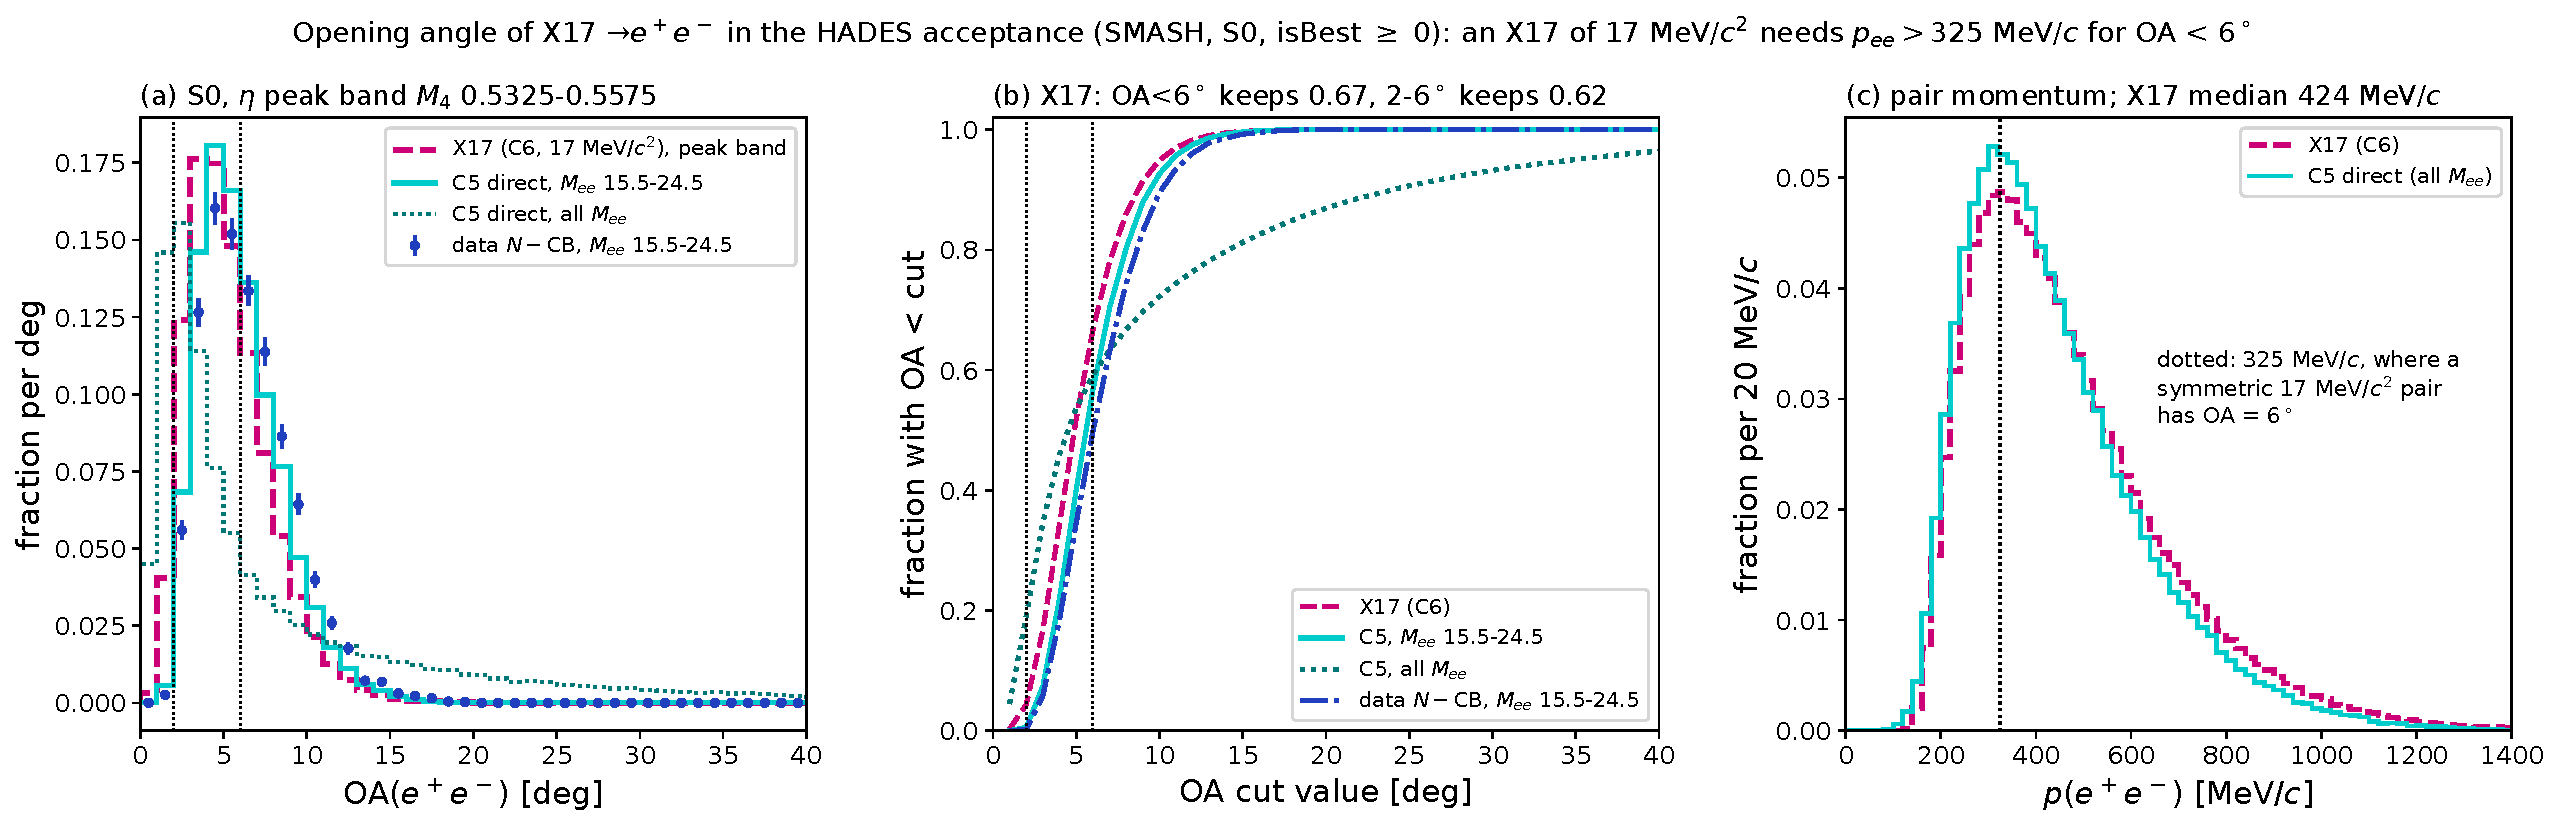
\includegraphics[width=\textwidth]{figs_all/e1_x17_oa_v2.pdf}
\caption{\textbf{What it shows: two thirds of the simulated X17 pairs have OA$<6^\circ$ because they are fast, and pairs of
the same mass from the direct decay look the same.} Selection: data and SMASH with the same cuts (Part~III's ``pre'' plus the pion-vertex cut) = PT3 trigger (at least two sectors with an inner-TOF hit in coincidence with TOF or RPC, and at least three inner-TOF paddles hit; trigger bit 8192 in the data, bit 8192 set in SMASH), event vertex in the target region ($z>-160$\,mm), \betanew particle identification (pions within $3\sigma$, leptons within $5\sigma$ and with a RICH ring), corrected momenta of all four tracks, all stored combinations of each event (isBest\,$\ge0$), both pions used in the event-vertex fit; $\eta$ peak band $0.5325\le M_4<0.5575$\,\GeVcc; SMASH: masses moved to the data scale of Part~III ($M_4\times0.99615$, $\Mpipi\times0.9952$), weights PDG branching ratios $\times$ V3, mode~A; X17 (class~6, 17\,\MeVcc) at all \Mee in the band; direct decays in the X17 window $15.5\le\Mee<24.5$\,\MeVcc and at all \Mee; data: counts in the X17 window minus the combinatorial background CB $=2\sqrt{N_{++}N_{--}}$ from the like-sign data with the same cuts (10\,\MeVcc cells of $M_4$, shared out over the OA bins by the like-sign share of each 50\,\MeVcc band, $k=1$); (c) simulation only, peak band, all \Mee. Later finding of Part~III (file \code{figs_all/e1_x17_oa_v2.pdf} of
\code{report_all.pdf}). (a) OA distributions, unit area: X17 (17\,\MeVcc,
dashed magenta), the direct decays in the X17 window $15.5\le\Mee<24.5$\,\MeVcc (cyan) and at all \Mee (dotted) and, as a
\emph{data} curve, the data after CB subtraction in the X17 window (blue points). (b) Fraction below an OA cut (same
curves; the dash-dotted blue line is data). (c) Pair momentum of X17 and of the direct decays (simulation only); dotted:
325\,\MeVc, where a symmetric 17\,\MeVcc pair has OA $=6^\circ$.}
\label{fig:s5x17oa}
\end{figure}

%----------------------------------------------------------------------
\subsection{Blind test of the signal extraction and of the X17 search}
\label{sec:s5blind}
%----------------------------------------------------------------------
\inshort{the template fit and the calibrated Gaussian fit recover the peak within $+1$ to $+6$\,\%, linear side
bands lose it; for the bump the side band with the simulated shape is closest; the X17 estimators are linear, but
only those whose error includes the background uncertainty give valid limits. Later finding (Part~III): this test
favoured the template fits; with the template noise of a real analysis they come out about 10\,\% low, and the
leak-corrected peak side bands and the bump edge step are the estimators that hold (note at the end of the $\eta$
results).}
The extraction methods planned for the data were tested on simulated pseudo-data whose true
content was hidden from the analyst until the procedure was frozen.

\textbf{Preparation.}
\begin{enumerate}
\item \textbf{Split.} The entries are split by event group: half A (even group number) gives the
      templates, half B (odd) gives the pseudo-data. Every entry of an event goes to the same half.
\item \textbf{Templates}: half A with weights $\times2$, histograms of \Mfour (1\,\MeVcc bins) per
      component and selection (PEAK, DIRECT, BUMP of Sect.~\ref{sec:s5opt} and the v1 X17 selection),
      exact window sums, and \Mee and $\Mfour\times\Mee$ for X17.
\item \textbf{$\eta$ pseudo-data}: 200 toys at $L_{\mathrm{toy}} = \Lsim/2 = 110.525\,\nbinv$ from a
      Poisson bootstrap of half B per event group. An event with largest entry weight $w_g$ enters
      $n\sim\mathrm{Poisson}(w_g)$ times; in each copy one uniform $u$ is drawn and each entry with
      $w_r/w_g>u$ is kept, so that every entry has the expected multiplicity $w_r$. Only T1+T2 entries
      are used. A check with 4000 toys gave toy variance / predicted variance = 0.95--1.06; the sum
      of the squared pulls of the variances over the 21 regions was 36.8. Repeated with eight further
      random seeds, this sum is 9.1--35.7, on average $20.7\pm10.1$ over all nine runs (21 expected; the
      spread is wider than for 21 independent entries because the selections share entries), and the
      variance ratio stays within 0.94--1.06: the bootstrap reproduces the variances, the value 36.8 is
      a fluctuation.
\item \textbf{X17 pseudo-data}: 1500 toys at \Ldata (UNCONFIRMED), parametric: in each cell of
      $\Mfour\times\Mee$ signal and background are drawn as Poisson numbers around the half-B
      expectation ($\times2\times\Ldata/\Lsim$). BR $\in\{0, 1, 3, 10, 30\}\times10^{-6}$, 300 toys
      each, shuffled, with random ids.
\item \textbf{Sealed key}: true counts per toy, group and region; the expectation of half B per
      toy, called $\mu$, is the quantity a measurement would estimate.
\end{enumerate}
For the weight rules~v2 the $\eta$ and X17 toys were drawn again with the same seed. Because
the weights changed, the random draws differ from those of rules~v1, so the biases and pulls
moved within their statistical errors (by up to 2.3 standard deviations).

\textbf{Methods} (frozen before any yield was computed on the pseudo-data). Peak yield: M1 =
Gaussian (fixed at 0.5460\,\GeVcc, 6.7\,\MeVcc; later, Part~III: the data peak is $5.44\pm0.60$\,\MeVcc wide,
\S\ref{sec:s5acc}) + second-order polynomial, calibrated with the
response to the half-A peak template; M2 = template fit (free normalisations of peak, bump and
background templates, binned Poisson likelihood with the template variance added); M2b = M2
with the background split into $G_\eta$ and the rest; M2d = M2 with the peak split into class 5
(free) and class 4 (constrained to its half-A value $\pm$ its MC error); M3 = linear side bands
(7.8\,\MeVcc on each side) with the signal leakage $\lambda$ into the side bands corrected,
$S = [N_{\mathrm{win}} - (N_L+N_U)/2\cdot25.4/7.8]/(1-\lambda)$; M3c = M3 with the curvature of
the background taken from half A. Bump yield: B1 = bifurcated Gaussian + $\eta$ Gaussian +
polynomial; B2 = the bump of M2; B3 = edge step in \Mfour; B4 = side band 0.5665--0.70 with
the background shape from half A. Direct yield: M2d, and D5 = split at $\Mee = 10$\,\MeVcc with a
$2\times2$ unfolding. X17: X1 = fit of \Mee in the window with free normalisations of the direct
decay and the rest; X2 = X1 with the raw half-A template; X3 = X1 on 8--40\,\MeVcc; X4 = X1 with
the direct-decay normalisation constrained to $1\pm0.10$; X5 = counting with $B$ from half A.
X4 and X5 were added after the X1 results were seen (declared, before their own results). An
example toy with the fits is shown in Fig.~\ref{fig:s5toy}.

\begin{figure}[!htbp]
\centering
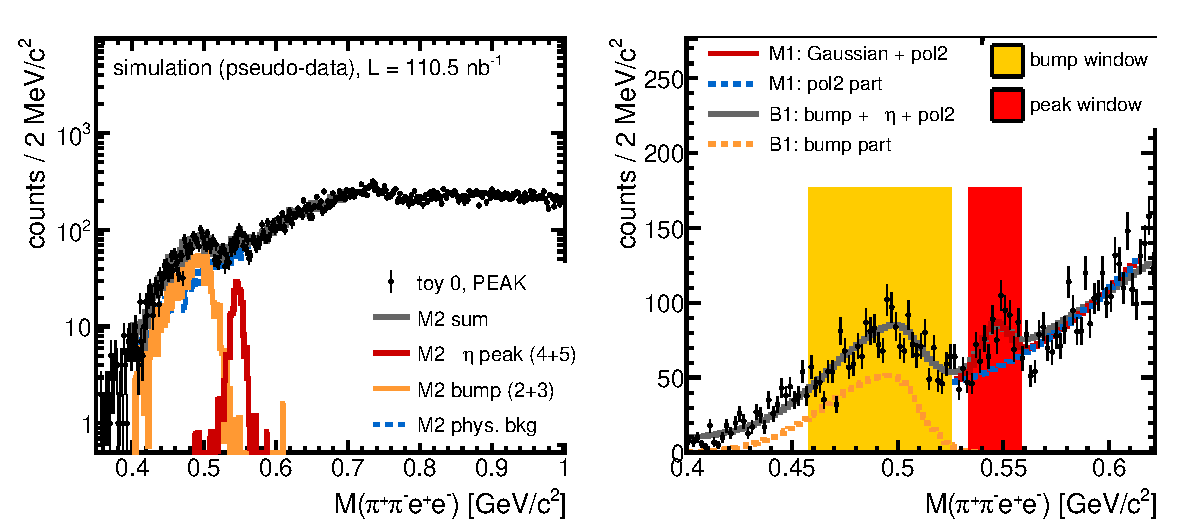
\includegraphics[width=\textwidth]{figs/s5_blind_ana_toy0_PEAK_cnt.pdf}
\caption{One $\eta$ toy (pseudo-data, $L = 110.5\,\nbinv$, PEAK selection). Selection: SMASH simulation only, no combinatorial background (mode~A, weights $\times$ V3); base selection ``pre'' = simulated PT3 trigger (bit 8192 set), event vertex in the target region ($z>-160$\,mm), particle identification by \betanew with the simulation polygons (pions within $3\sigma$, leptons within $5\sigma$ and with a RICH ring), energy-loss-corrected momenta of all four tracks, all stored \ppee combinations per event (isBest\,$\ge0$); pseudo-data = Poisson bootstrap of half~B (odd event groups) of the T1+T2 counts after ``pre'' with $0.30\le\Mfour<1.20$\,\GeVcc; templates from half~A (even event groups), scaled to 110.5\,\nbinv; frozen PEAK selection = ``pre'' plus both pion tracks within 40\,mm of the event vertex along the beam ($\Delta z_\pi<40$\,mm) and missing mass of \ppee below 2.85\,\GeVcc ($\mathrm{MM}_4$, computed with $T=4530$\,MeV); 2\,\MeVcc bins; fit ranges M2 0.400--0.700, M1 0.526--0.614 and B1 0.400--0.620\,\GeVcc; shaded: bump window $0.4576\le\Mfour<0.5255$\,\GeVcc and peak window $0.5333\le\Mfour<0.5587$\,\GeVcc (simulation mass scale). Left: \Mfour with
the components of the template fit M2. Right: zoom with the Gaussian + polynomial fit M1 and the
bump fit B1, with the bump and peak windows.}
\label{fig:s5toy}
\end{figure}

\textbf{What a bias means here.} The templates (half A) and the pseudo-data (half B) are two
statistically independent copies of the same model. The truth of half B differs from half A by
MC fluctuations: peak (PEAK selection) $241.4$ against $224.1\pm10.3$ counts (+7.7\,\%), bump (BUMP)
1095.6 against $1046.1\pm35.7$ (+4.7\,\%), class 5 (DIRECT) 128.88 against $128.00\pm0.48$, class 4
(DIRECT) 118.5 against $106.2\pm10.5$ (+11.5\,\%). All toys share this difference. A method bias
can therefore be resolved only beyond the common MC error, which is $\pm$11--15\,\% for the peak and
$\pm$4.5--5\,\% for the bump.

\begin{table}[H]
\centering
\caption{Blind test, $\eta$ yields (200 toys). Bias = $\langle Y\rangle - \mu$ with the error of the
mean over toys and the common MC error (template and parent sample). Pull = $(Y-\mu)/\sigma_{\mathrm{tot}}$
with the error quoted by the analyst (mean/rms). Coverage: fraction of toys with
$|Y-\mu|\le\sigma_{\mathrm{tot}}$ (nominal 0.683).}
\label{tab:s5blind}
\footnotesize
\setlength{\tabcolsep}{4pt}
\begin{tabular}{@{}l l r r c c@{}}
\toprule
yield, selection ($\mu$) & method & bias [counts] & relative & pull & coverage \\
\midrule
peak, PEAK (241.4)  & M1 Gauss + pol2   & $+7.4\pm2.9\pm31.3$  & $+3.1$\,\%  & $+0.17$ / 0.96 & 0.72 \\
                    & M2 template fit   & $+3.4\pm2.0\pm27.5$  & $+1.4$\,\%  & $+0.08$ / 0.80 & 0.77 \\
                    & M2b               & $+10.4\pm2.2\pm30.6$ & $+4.3$\,\%  & $+0.26$ / 0.82 & 0.74 \\
                    & M3 side bands     & $-51.0\pm3.9\pm45.3$ & $-21.1$\,\% & $-0.86$ / 0.93 & 0.53 \\
                    & M3c               & $-124.5\pm3.9\pm56.9$ & $-51.6$\,\% & $-1.82$ / 0.80 & 0.16 \\
\midrule
bump, BUMP (1095.6) & B4 side band & $+42.3\pm3.9\pm54.9$ & $+3.9$\,\% & $+0.61$ / 0.79 & 0.66 \\
                    & M2 template fit   & $+84.5\pm3.4\pm49.7$ & $+7.7$\,\%  & $+1.34$ / 0.76 & 0.31 \\
                    & B1 parametric     & $+59.0\pm7.1\pm78.6$ & $+5.4$\,\%  & $+0.56$ / 0.96 & 0.66 \\
                    & B3 edge step      & $+13.8\pm13.3\pm171.5$ & $+1.3$\,\% & $+0.01$ / 0.86 & 0.76 \\
\midrule
direct, DIRECT (128.9) & M2d (cl.\ 4 constr.) & $+26.6\pm2.2\pm31.0$ & $+20.6$\,\% & $+0.68$ / 0.79 & 0.62 \\
                    & D5 (\Mee split)   & $+40.5\pm3.9\pm39.3$ & $+31.4$\,\% & $+0.70$ / 0.96 & 0.61 \\
\bottomrule
\end{tabular}
\end{table}

\textbf{$\eta$ results} (Table~\ref{tab:s5blind}, Fig.~\ref{fig:s5bias}).
\begin{itemize}
\item \textbf{Peak.} The template fit M2 and the calibrated Gaussian fit M1 find the peak within
      +1 to +6\,\% in all three selections, well inside the common MC error. Per toy they differ by
      about 12\,\% (rms 29 counts), so a difference of that size between them in data is normal.
      M2b is 3--8\,\% above M2 every time.
\item \textbf{Linear side bands (M3) lose the peak}, because the background is convex under it and
      17\,\% of the signal leaks into the side bands. Two independent realisations of the MC noise
      measure this: the half-B toys give $-21$\,\%, $-13$\,\%, $-16$\,\% and the exact half-A sums
      (Asimov) $-40$\,\%, $-43$\,\%, $-46$\,\% (PEAK, DIRECT, BUMP); the mean is about $-30\pm14$\,\%.
      The MC-calibrated version M3c over-corrects ($-44$ to $-52$\,\%), because the curvature from
      the simulation is itself noisy.
\item \textbf{Bump.} B4 is closest (+3 to +4\,\%); the template fit agrees within 3--8\,\%; the
      parametric fit B1 comes out 5--10\,\% high; the edge step B3 is unbiased but has 15--17\,\%
      statistical error.
\item \textbf{Direct decay alone.} \Mfour cannot separate class 5 from class 4. M2d gives
      class 4 = 105.4 (truth 118.5) and therefore class 5 too high by the same amount
      ($26.6 = 13.5 + 13.1$ counts). The split is limited by the simulation statistics of the
      conversion peak ($N_{\mathrm{eff}}\approx100$ in a half). \emph{Later (Part~III):} its X17 fit of
      $\Mfour\times\Mee$, run on the X17 toys of this section, gave the direct-decay yield 55\,\% too high (11\,168 against
      7\,200 at $\mathrm{BR}=0$); the cause is the same, the heavy entries of the simulated parent sample (Fig.~\ref{fig:s5side}).
\item \textbf{Errors.} The event-group errors describe the spread of the toys: the ratio rms/error
      is 0.93--1.08 for M1, M3, B1, B3 and D5 and 0.90--1.06 for the template fits and B4, so the
      errors are adequate. The common MC error is not in the per-toy error and must be added.
\end{itemize}

\notebox{\textbf{Later finding (Part~III, \code{report_all.pdf}, section ``Validation of the estimators on simulation''):
the recommendations of this test do not hold with realistic template noise} (Fig.~\ref{fig:res_stress}). Part~III ran
about 160\,000 estimator chains on pseudo-data at the data luminosity, with a CB built from the like-sign pairs of the data,
in several truth scenarios and template configurations.
\begin{itemize}\setlength{\itemsep}{0pt}
\item \textbf{The split of this test moves the results by itself.} Templates from half A and truth from half B is the
      configuration used here. The two halves of the smoothed simulated background differ by 5--10\,\% per 50\,\MeVcc band;
      this single difference moves the $\eta$ scale by $+32$\,\% (and by $-37$\,\% with the halves swapped) and B4 by
      $+27$/$-31$\,\%. The template-to-truth difference then has four times the variance of the real analysis. The common
      MC error of this section ($\pm$11--15\,\% peak, $\pm$4.5--5\,\% bump) is this kind of effect.
\item \textbf{Realistic template noise biases every template fit low.} With the truth from the full sample and the
      templates from bootstrap copies, the template fits give the $\eta$ scale $-10.1$\,\%, the bump $-11.6$\,\%, the peak
      $-6.6$\,\% and the branching ratio of the direct decay $+14.8$\,\%. The cause is the noise of the raw signal templates
      (effective 10--200 entries per histogram): a fit that scales a noisy template is pulled towards zero (errors in the
      regressor). Estimators that do not scale a signal template are not attenuated: B4 $-1.4$\,\%, peak side bands
      $-0.5$\,\%. Template noise alone gives $\chi^2/\mathrm{ndf}$ = 2--3 for a perfect model (2.83 for the main template
      fit, 2.10 for the background fit).
\item \textbf{The peak.} Part~III's main estimator is a side band like M3, but with the ratio of the background in the
      window and in the side bands taken from the smoothed simulation (fitted to the data) and with the leak of the peak
      into the side bands corrected. M3c over-corrected here because its curvature came from the noisy raw templates.
\end{itemize}}

\notebox{\textbf{Later finding (Part~III), continued: the bump and the fits with several scales.}
\begin{itemize}\setlength{\itemsep}{0pt}
\item \textbf{The bump.} The edge step B3 (here unbiased, 15--17\,\% error) became the basis of Part~III's bump measurement (the per-slice step is now its cross-check, D37): it closes
      within 2\,\% on 16\,000 pseudo-data sets, and the quadratic background term that moves B4 by $+150$\,\% moves it by
      only $-2.1$\,\%. It is limited by the simulation statistics (MC error 11\,\%; taking the simulated step from the bump
      classes alone, without a smoothing model, gives about 6.6\,\%). B4 ($+3.9$\,\% here) is NOT DETERMINED in the data: its
      background has to be carried down 40--120\,\MeVcc from above the peak.
\end{itemize}}

\notebox{\begin{itemize}\setlength{\itemsep}{0pt}
\item \textbf{The edge in the distance to it, $u$} (Part~III, package ``edgeu'', verified). The largest \Mfour that
      $\eta\to\pipi\piz$, $\piz\to\ee\gamma$ can give with the photon lost, $E(\Mpipi,\Mee)$, depends on both pair masses;
      in $u=\Mfour-E(\Mpipi,\Mee)$ all edges fall on $u=0$ (Fig.~\ref{fig:s5edgeu}). In the simulated truth every bump count
      lies below its exact edge (largest excess $-0.48$\,\MeVcc for class~2, $-0.51$ for class~3); without the \Mee term
      3.8\,\% of class~2 would lie above it. The reconstructed $u$ is smeared by 6.7\,\MeVcc at the edge (Gaussian core of a
      fit on $\pm40$\,\MeVcc; 5.8--7.1\,\MeVcc depending on the fit method), almost all from the \Mfour error (the edge
      function adds 1.2\,\MeVcc). The simulated non-$\eta$ backgrounds show no step at $u=0$ (\piz Dalitz and vector-meson
      pairs $12\pm140$, conversion pairs $59\pm148$ counts); the other $\eta$ counts give a raw step of $123\pm53$ counts
      (2.3$\sigma$) without any visible structure, treated as template noise. The $e^-e^-$ like-sign counts of the data step
      at $u=0$ ($73.5\pm15.7$, $4.7\sigma$).
\end{itemize}}

\notebox{\begin{itemize}\setlength{\itemsep}{0pt}
\item[] Part~III (package ``eestep'', D39, approved by the analyst on 15 November 2026)
      traced this step to lepton pairs from the two photons of the \piz in $\eta\to\pipi\piz$ (a Dalitz lepton and a
      conversion lepton of the other photon, or two conversion leptons): a kinematic toy of $4\times10^5$ decays per topology
      gives them exactly the bump's edge (true $u$ never above 0; median \Mee near it 113--121\,\MeVcc). The standard set (the
      only one with $\eta\to\pipi\piz$) contains such pairs, mostly $e^-e^-$, at large \Mee (around 100\,\MeVcc) and wide
      opening angles (around $40^\circ$); part of the $e^-e^-$ ones carry a Compton or knock-on electron of a photon, which is
      always negative and has no positive counterpart. They serve only to identify the origin of the data step: the
      simulation does not model the like-sign or combinatorial background, so no like-sign rate of the data is compared with
      it, and no SMASH number enters a correction or the CB (the CB is kept, D39).
      Charge flips are rare: a true \ee pair appears as a like-sign entry in 0.04\,\% (standard set), 0.01\,\% (lepton set) and
      0.008\,\% ($\eta$ set) of the cases; per true $e^+$ a negative charge is reconstructed for 1.7\,\% below 100\,MeV$/c$,
      0.46\,\% at 100--200, 0.10\,\% at 200--300 and at most 0.06\,\% above. An independent verifier confirmed the mechanism
      (also for the Compton electrons, which have the same edge). In the data the one fit in $u$ gives
      $0.426\pm0.020\pm0.034\pm0.030$ of SMASH (class-2 angle corrected with per-count QED weights, D38; the peak-tail term of
      D40 in the systematic error), with MC error 7.0\,\% (simulated step from the bump classes alone) against 4.7\,\%
      statistical; it is Part~III's bump measurement, and the per-slice edge is its cross-check (D37). D37--D40 were approved
      by the analyst on 15 November 2026.
\item \textbf{Fits with several scales} suffer the same attenuation: Part~III's flexible fit with a free scale per channel
      biases class~2 by $-20$\,\% and class~4 by $-58$\,\% on pseudo-data; the common $\eta$ scale it finds in the data goes
      from 0.46 to 0.57 after the template-noise correction.
\end{itemize}}

\begin{figure}[!htbp]
\centering
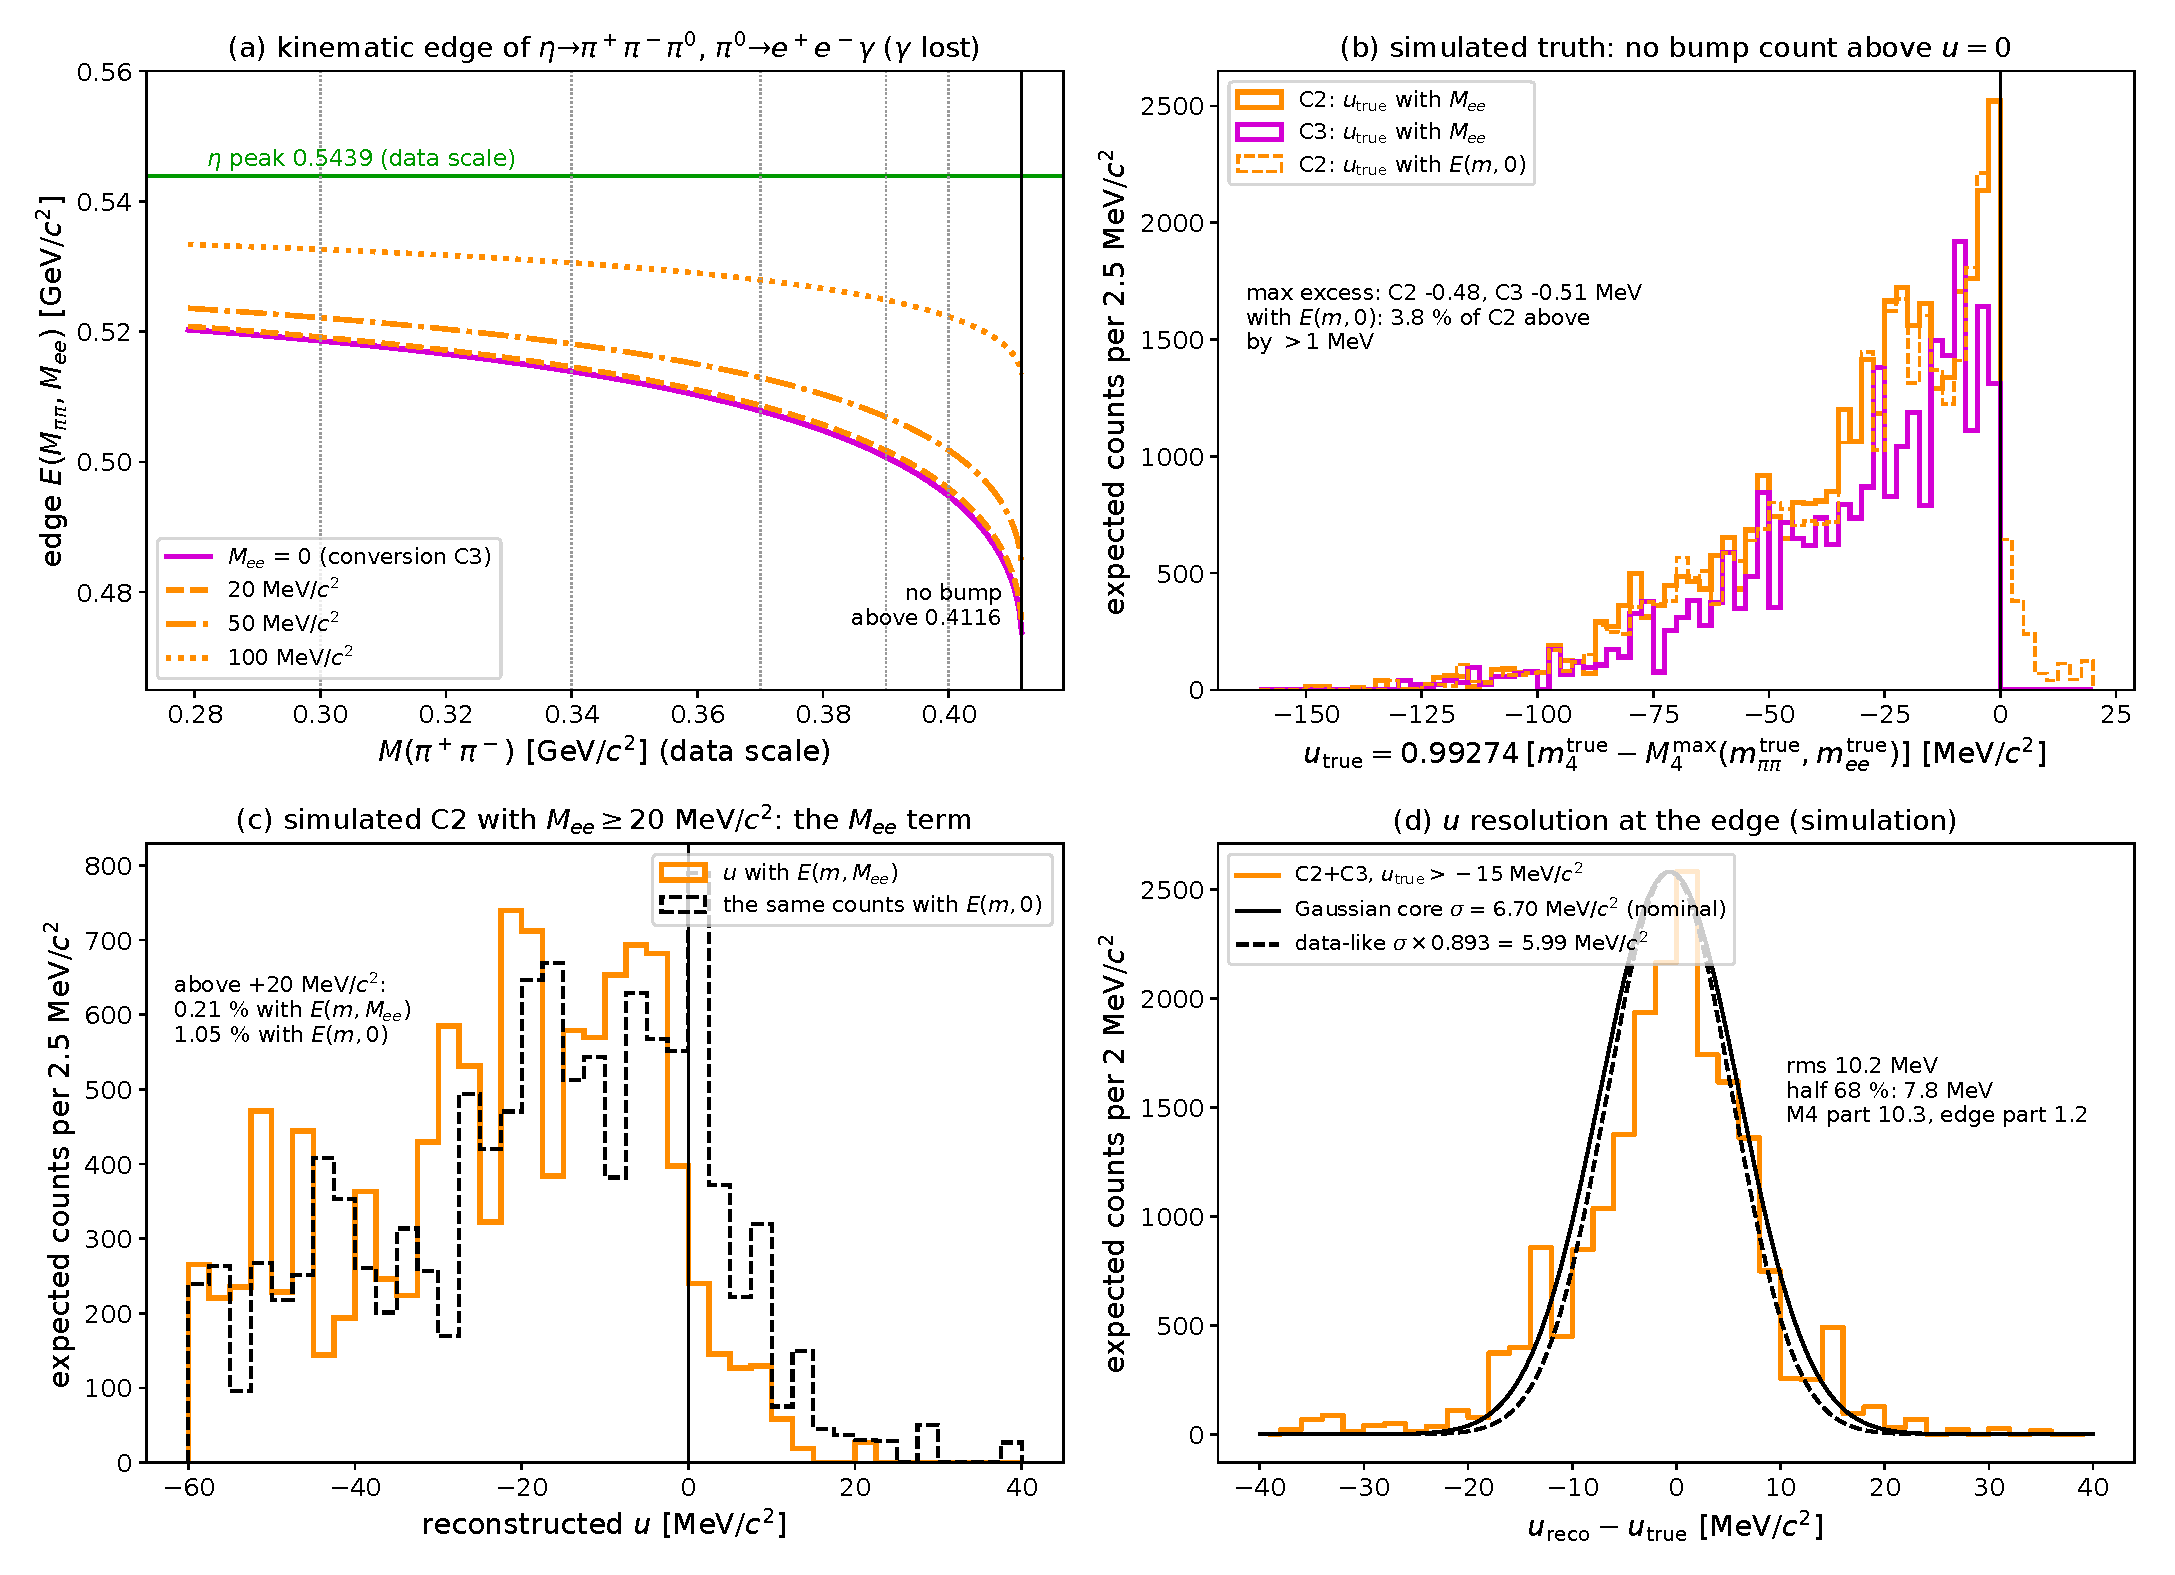
\includegraphics[width=0.92\textwidth]{figs_all/edgeu_kinematics_cnt.pdf}
\caption{\textbf{What it shows: the edge of the bump depends on \Mpipi and \Mee, and once both are taken into account no
simulated bump count lies above it; the reconstructed distance to the edge, $u$, is smeared by 6.7\,\MeVcc.} Selection: SMASH simulation only (mode~A, weights PDG branching ratios $\times$ V3, no QED angle correction of class~2); Part~III's ``pre'' plus the pion-vertex cut = simulated PT3 trigger (bit 8192 set), event vertex in the target region ($z>-160$\,mm), \betanew particle identification (pions within $3\sigma$, leptons within $5\sigma$ and with a RICH ring), corrected momenta of all four tracks, all stored combinations of each event (isBest\,$\ge0$), both pions used in the event-vertex fit; masses on the data scale of Part~III, $M_4'=0.99615\,M_4$, $\Mpipi'=0.9952\,\Mpipi$; expected raw counts at 6079.2\,\nbinv; (a) the edge function only, no counts; (b)--(d) classes 2 and 3 with $0.30\le\Mpipi'<0.40$\,\GeVcc; (c) class~2 with reconstructed $20\le\Mee<135$\,\MeVcc ($u$ is not defined above the \piz mass); (d) classes 2+3 with $u_{\mathrm{true}}>-15$\,\MeVcc and reconstructed $\Mee<135$\,\MeVcc. Later finding
of Part~III (file \code{figs_all/edgeu_kinematics_cnt.pdf} of \code{report_all.pdf}). (a) The edge $E(\Mpipi,\Mee)$ for $\Mee=0$, 20, 50,
100\,\MeVcc; green: the $\eta$ peak; dotted: the \Mpipi slices of the per-slice edge fit; no bump above
$\Mpipi=0.4116$\,\GeVcc. (b) Simulated truth $u_{\mathrm{true}}$ for class~2 (orange) and class~3 (magenta); dashed: class~2
with the edge at $\Mee=0$, which puts counts above $u=0$. (c) Reconstructed $u$ of class~2 with $\Mee\ge20$\,\MeVcc, with the
\Mee term (orange) and without it (dashed). (d) $u_{\mathrm{reco}}-u_{\mathrm{true}}$ near the edge (classes 2+3,
$u_{\mathrm{true}}>-15$\,\MeVcc): template width 6.70\,\MeVcc (Gaussian fit on $\pm40$\,\MeVcc; 5.8--7.1\,\MeVcc depending on
the fit method); dashed: the width $\times0.893$ favoured by the data peak (Part~III).}
\label{fig:s5edgeu}
\end{figure}

\begin{figure}[!htbp]
\centering
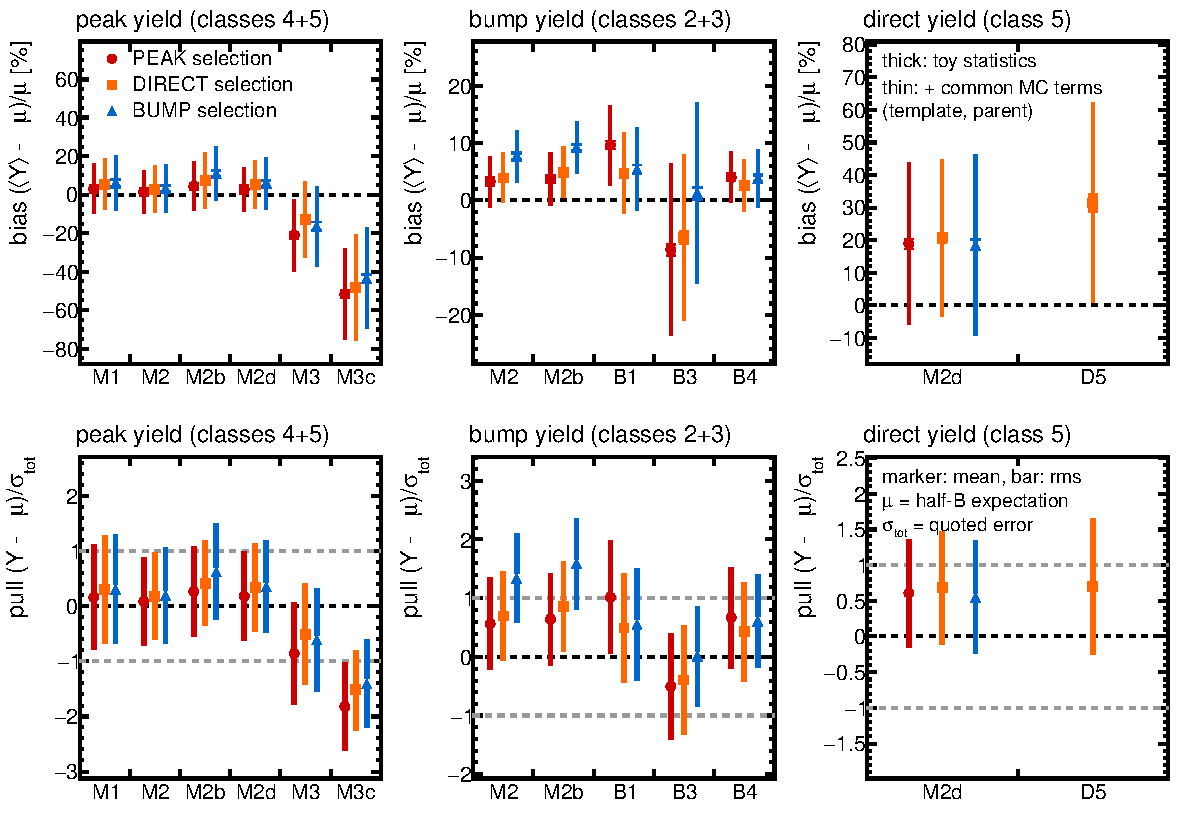
\includegraphics[width=\textwidth]{figs/s5_blind_eval_eta_bias.pdf}
\caption{Blind test, $\eta$ yields. Selection: SMASH simulation only, no combinatorial background (mode~A, weights $\times$ V3); base selection ``pre'' = simulated PT3 trigger (bit 8192 set), event vertex in the target region ($z>-160$\,mm), particle identification by \betanew with the simulation polygons (pions within $3\sigma$, leptons within $5\sigma$ and with a RICH ring), energy-loss-corrected momenta of all four tracks, all stored \ppee combinations per event (isBest\,$\ge0$); 200 pseudo-data sets at $L=110.525$\,\nbinv, pseudo-data = Poisson bootstrap of half~B (odd event groups) of the T1+T2 counts after ``pre'' with $0.30\le\Mfour<1.20$\,\GeVcc; templates from half~A (even event groups); markers for the three frozen selections: PEAK = ``pre'' plus both pion tracks within 40\,mm of the event vertex along the beam ($\Delta z_\pi<40$\,mm) and missing mass of \ppee below 2.85\,\GeVcc ($\mathrm{MM}_4$, computed with $T=4530$\,MeV); DIRECT = ``pre'' plus the 40\,mm pion cut only; BUMP = ``pre'' only; yields: peak = classes 4+5 in the peak window $0.5333\le\Mfour<0.5587$\,\GeVcc, bump = classes 2+3 in the bump window $0.4576\le\Mfour<0.5255$\,\GeVcc, direct = class~5 in the peak window ($\mu$ = their half-B expectation). D5 (shown with DIRECT) uses instead the counts of ``pre'' with both pions used in the event-vertex fit, split at $\Mee=10$\,\MeVcc. Side bands: M3 and M3c 0.5255--0.5333 and 0.5587--0.5665\,\GeVcc, B4 0.5665--0.700\,\GeVcc. Top: relative bias $(\langle Y\rangle-\mu)/\mu$ per method and
selection; thick bars: toy statistics, thin bars: including the common MC terms. Bottom: pull
$(Y-\mu)/\sigma_{\mathrm{tot}}$, marker = mean, bar = rms.}
\label{fig:s5bias}
\end{figure}

\textbf{X17 results} (Table~\ref{tab:s5blindx}, Figs.~\ref{fig:s5side} and~\ref{fig:s5x17lin}).
Each standard-set entry of half B stands for about 55 expected data counts. The background of every X17 toy
is therefore the unsmoothed half-B content, with single-bin spikes of 50--200 counts that all toys
share and that differ from half A (Fig.~\ref{fig:s5side}).
\begin{itemize}
\item Every estimator follows the injected BR with a slope of 0.98--1.02.
\item The zero point is shifted, by the same amount in all toys: it is set by how well the
      background under the line is known. Counting with the half-A background (X5) closes exactly:
      the predicted shift $(B_B-B_A)/s_1 = (7947.8-8268.2)/2.725\times10^{7} = -11.76\times10^{-6}$
      is measured as $-11.66\pm0.19\times10^{-6}$ at $\mathrm{BR}=0$.
\item Only estimators whose error contains this background uncertainty give valid limits (X1, X4,
      X5 cover the true BR at every BR). Their median limits at $\mathrm{BR}=0$ are
      $2.1$--$6.2\times10^{-5}$, 4--11 times the $\mathrm{UL}_{\mathrm{stat}}$ of v1, and consistent
      with the $1.9\times10^{-5}$ of Eq.~(\ref{eq:s5ul}).
\item Estimators with a small error (X2, X3, X1 with the statistical error only) exclude the true
      BR. No estimator claimed a $3\sigma$ signal at $\mathrm{BR}=0$, but only because the common shift
      happens to be negative: with the opposite sign X2 and X3 would claim one in 100\,\% and 98\,\%
      of the toys.
\end{itemize}

\begin{table}[H]
\centering
\caption{Blind test, X17 (1500 toys at $\Ldata = 6080.5\,\nbinv$, UNCONFIRMED; BR in $10^{-6}$).
Offset: mean extracted BR at injected $\mathrm{BR}=0$. Coverage: fraction of toys whose UL is above
the injected BR. X1--X3 were frozen; X4 (X1 with the direct-decay normalisation $a_D$ constrained) and X5
(counting) were added after the freeze.}
\label{tab:s5blindx}
\footnotesize
\setlength{\tabcolsep}{4pt}
\begin{tabular}{@{}l c c c c@{}}
\toprule
estimator & offset at 0 & slope & median UL at 0 (16--84\,\%) & UL coverage at 0 / 3 / 10 / 30 \\
\midrule
X1 window fit         & $-72.7\pm0.5$ & $1.004\pm0.021$ & 31.2 (28.2--34.4) & 1.00 / 1.00 / 1.00 / 0.99 \\
X2 raw template       & $-72.4\pm0.6$ & $0.977\pm0.024$ & 2.5 (2.1--3.3)    & 1.00 / 0.34 / 0.00 / 0.00 \\
X3 8--40\,\MeVcc     & $-74.9\pm0.3$ & $0.996\pm0.011$ & 12.7 (11.8--13.5) & 1.00 / 1.00 / 1.00 / 0.00 \\
X4 X1, $a_D = 1\pm0.1$ & $-1.1\pm0.4$  & $1.016\pm0.018$ & 61.8 (57.3--67.3) & 1.00 at all BR \\
X5 counting                   & $-11.7\pm0.2$ & $0.999\pm0.008$ & 21.1 (19.7--22.7) & 1.00 at all BR \\
\bottomrule
\end{tabular}
\end{table}

\begin{figure}[!htbp]
\centering
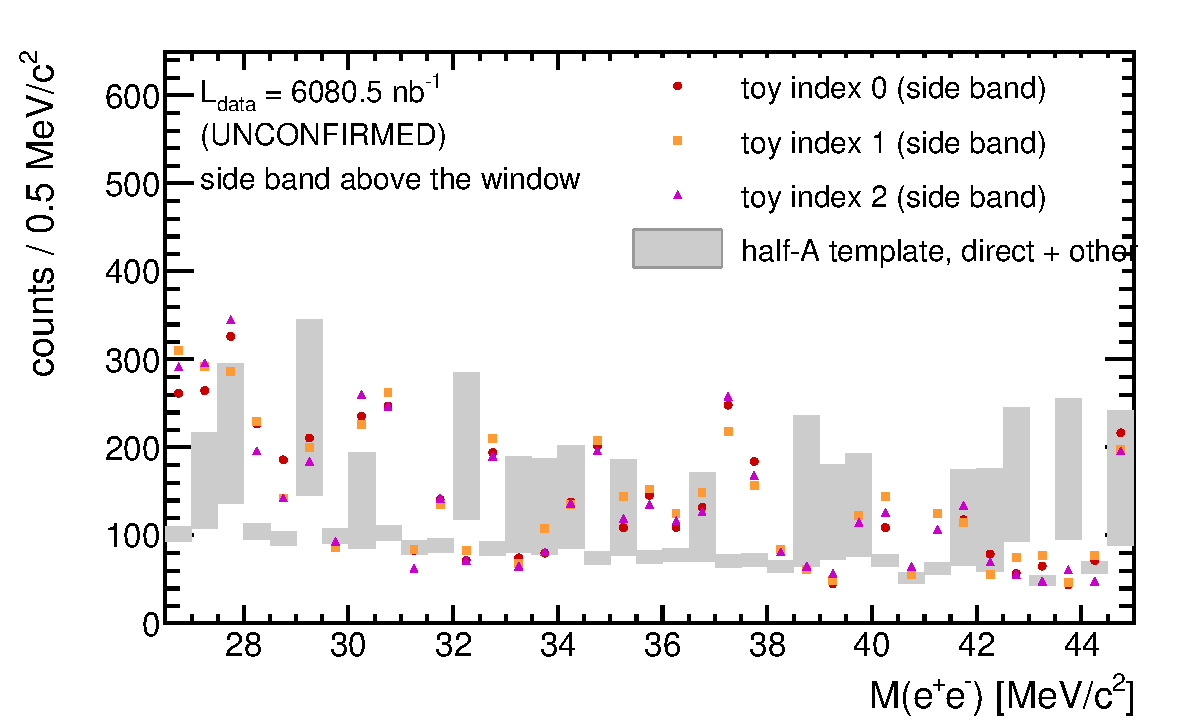
\includegraphics[width=0.75\textwidth]{figs/s5_blind_ana_x17_sideband_cnt.pdf}
\caption{\Mee side band (above the X17 window) of three X17 toys against the half-A template
(grey boxes). Selection: SMASH simulation only, no combinatorial background (mode~A, weights $\times$ V3); base selection ``pre'' = simulated PT3 trigger (bit 8192 set), event vertex in the target region ($z>-160$\,mm), particle identification by \betanew with the simulation polygons (pions within $3\sigma$, leptons within $5\sigma$ and with a RICH ring), energy-loss-corrected momenta of all four tracks, all stored \ppee combinations per event (isBest\,$\ge0$); X17 selection v1 of the blind test = ``pre'' plus both pions used in the event-vertex fit and $0.5330\le\Mfour<0.5555$\,\GeVcc; side band $26.5\le\Mee<45$\,\MeVcc in 0.5\,\MeVcc bins, above the v1 X17 window $13.0\le\Mee<26.5$\,\MeVcc; toys: Poisson draws around the half-B expectation of T1 (without X17) plus T2, plus X17 at a hidden BR, scaled to \Ldata; template: half~A, direct decay plus all other background. All toys show the same spikes, which come from single heavy entries of half B.
$\Ldata = 6080.5\,\nbinv$ (UNCONFIRMED).}
\label{fig:s5side}
\end{figure}

\begin{figure}[!htbp]
\centering
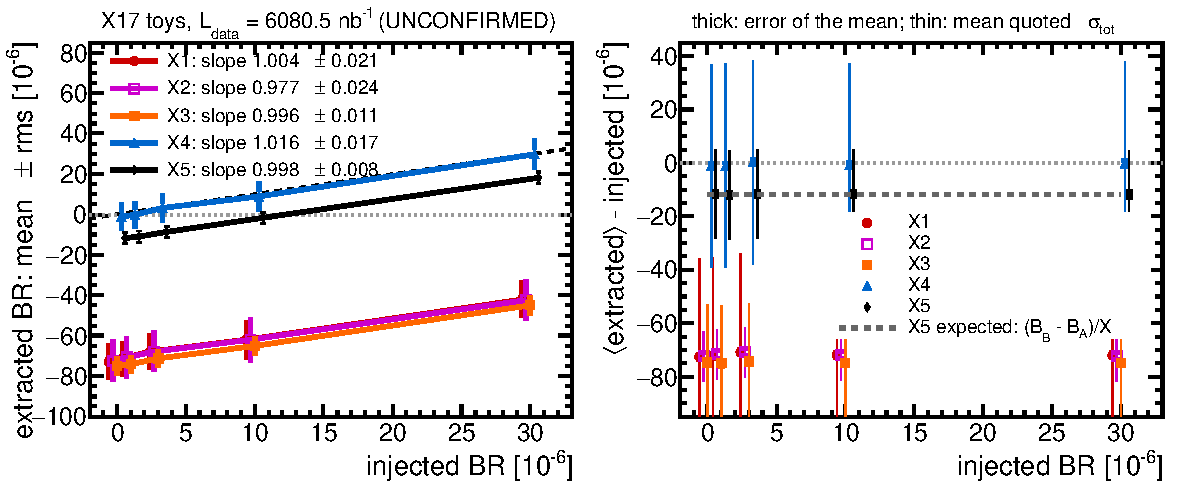
\includegraphics[width=\textwidth]{figs/s5_blind_eval_x17_linearity.pdf}
\caption{Blind test, X17. Selection: SMASH simulation only, no combinatorial background (mode~A, weights $\times$ V3); base selection ``pre'' = simulated PT3 trigger (bit 8192 set), event vertex in the target region ($z>-160$\,mm), particle identification by \betanew with the simulation polygons (pions within $3\sigma$, leptons within $5\sigma$ and with a RICH ring), energy-loss-corrected momenta of all four tracks, all stored \ppee combinations per event (isBest\,$\ge0$); 1500 pseudo-data sets at \Ldata (300 for each injected BR of 0, 1, 3, 10 and $30\times10^{-6}$; Poisson draws around the half-B expectation); X17 selection v1 of the blind test = ``pre'' plus both pions used in the event-vertex fit and $0.5330\le\Mfour<0.5555$\,\GeVcc; estimators on \Mee: X1, X2 and X4 fit $13.0\le\Mee<26.5$\,\MeVcc, X3 fits $8\le\Mee<40$\,\MeVcc, X5 counts in $13.0\le\Mee<26.5$\,\MeVcc. Left: extracted against injected BR (mean $\pm$ rms over 300 toys) with
straight-line fits. Right: mean offset; thick bars: error of the mean, thin bars: mean quoted
error. Dotted: the offset predicted for X5. $\Ldata = 6080.5\,\nbinv$ (UNCONFIRMED).}
\label{fig:s5x17lin}
\end{figure}

\textbf{Limits of this test.} The test is a closure test inside one model. It does not show how
the methods behave in data.
\begin{itemize}
\item Templates and pseudo-data come from the same SMASH model; there is no CB and no data/SMASH
      shape difference (0.87--1.36 above 0.56\,\GeVcc in earlier comparisons). Template fits are
      favoured by construction. $L_{\mathrm{toy}}$ is 55 times below \Ldata. \emph{Later (Part~III):} without any
      adjustment data/SMASH is 0.74--1.27 across \Mfour (one common scale leaves $\chi^2/\mathrm{ndf}=12$); and the
      template noise of the halves favours or disfavours the fits by itself (note above).
\item \emph{Later (Parts~II, III):} the simulation has no collisions outside the liquid-hydrogen cell (no target walls,
      no beam halo). In the data the target walls give 13--15\,\% of the counts after CB subtraction in
      0.40--0.70\,\GeVcc, with a softer \Mfour spectrum than the hydrogen, but only $3^{+4}_{-3}$\,\% of the $\eta$; the
      pseudo-data of this test contain no such component (\S\ref{sec:resnotdet}).
\item \textbf{The test was not blind by construction.} The frozen tables that the analyst read
      contain full-sample (A+B) numbers; together with the half-A templates they give the half-B
      truth (for example the PEAK yield 241.4 and the X17 background of half B). No sign was found
      that these numbers were used, and the sealed key was not read before the results were
      written, but the leak was possible.
\item The bootstrap repeats identical entries; how often an entry recurs across toys reveals its set and
      therefore class 4 (std) against class 5 ($\eta$ set). This was not exploited, but it is a
      second possible leak.
\item The X17 part used the v1 selection, whose \Mfour window was optimised (partly on a step of
      4 to 8 standard-set entries); the fixed window raises $\mathrm{UL}_{\mathrm{stat}}$ by 3\,\%.
\end{itemize}

%----------------------------------------------------------------------
\subsection{What this means for the data analysis}
\label{sec:s5data}
%----------------------------------------------------------------------
\begin{enumerate}
\item \textbf{Cuts.} In the simulation the four $\eta$-selection cuts remove background outside the
      windows but do not improve the windows themselves; OA$>2^\circ$ and $\alpha_\eta>140^\circ$ cost
      signal (conversions, bump). Their use in data must be justified by the CB and checked there.
      The pion-vertex cuts are the only ones with a gain inside the windows (4--6\,\%); the frozen
      PEAK and DIRECT cuts need the pion track $z$ in the compact data entries, otherwise ``pre + pions
      in vertex fit'' is the alternative. \emph{Later (Parts~II, III):} checked in the data: the CB is small
      (CB$/N$ = 0.07--0.10 in the peak window), OA$>2^\circ$ keeps 0.78 of the peak and lowers the precision in every
      selection, the kinematic cuts add nothing once the vertex cut is in, and the frozen PEAK gains as much as the best
      rule tuned blind on the data. The usual cuts are not applied (Part~III, D34).
\item \textbf{Peak extraction.} Template fit (M2) and Gaussian + polynomial with calibration (M1)
      close within a few per cent in simulation; a difference of about 12\,\% between them is normal.
      Linear side bands under the peak lose 13--46\,\% (about 30\,\% on average) and should not be used.
      \emph{Superseded (Part~III):} with realistic template noise the template fits come out about 10\,\% low; the main
      estimator is a side band with the background ratio from the smoothed simulation and the leak of the peak corrected.
\item \textbf{Bump.} Side band with the simulated background shape (B4) and template fit; the
      parametric fit tends to be high. \emph{Superseded (Part~III):} the bump is measured through the edge step (B3);
      B4 is not determined in the data. Part~III also measures the step in the distance to the edge, $u$ (0.426 of
      SMASH), its bump measurement; the per-slice step is the cross-check (D37, approved by the analyst on 15 November 2026).
\item \textbf{Direct decay alone.} The split of the peak into class 5 and class 4 is limited by the
      307 standard-set entries of class 4; the quoted error must include the simulation statistics.
\item \textbf{Simulation statistics.} The std set limits the bump and conversion templates
      ($N_{\mathrm{eff}}$ 270--1332) and the X17 background. The common MC error must be added to every
      yield. \emph{Confirmed later (Part~III):} its template-statistics error is 1.6--3.6 times the statistical error for
      the template fits, about 2 for the bump edge and 1--8 for its flexible fit; the effective number of simulated
      entries per histogram of its main fit is 1\,782--7\,141, and the rms of its simulation replicas equals the event-group
      error (ratio 0.989--1.016).
\item \textbf{X17.} With the background taken from this simulation the expected limit is about
      $2\times10^{-5}$ (at $\Ldata$ UNCONFIRMED), set by the simulation statistics of the background;
      $5.7\times10^{-6}$ would need the background known exactly. Any X17 estimate must carry the
      background uncertainty in its error. A larger std production or a background determined from
      data side bands would be needed to approach the statistical limit. \emph{Later (Part~III):} done with the
      background from the data side bands: observed limit $3.16\times10^{-5}$ (PDG 2026; the frozen PDG 2020 value:
      footnote~\ref{fn:x17pdg}), expected $2.68\times10^{-5}$ (\S\ref{sec:s5x17}).
\end{enumerate}

\tipbox{\textbf{Open points of this section.} (i) $\Ldata$ is UNCONFIRMED. (ii) The absolute
efficiencies rest on $N_{\mathrm{direct}} = 100\times1\,181\,801$ (representativeness of the 1000
generator files UNVERIFIED; later, Part~III: a 40-file count gives $1.0690\pm0.0035$\,mb). (iii) The X17 \Mpipi
distribution and decay angle are assumed (phase space, isotropic). (iv) The blind test should be repeated with cut
definitions only, with hidden per-toy signal scales and with pseudo-data that do not repeat identical entries; a version with
a CB-like component and a reweighted background shape would test the methods closer to data (later, Part~III: done with
realistic template noise and a CB from the data, note in \S\ref{sec:s5blind}).
(v) The pion-vertex variables were not compared between simulation and data (later, Part~II: the pion-vertex cut is as
efficient in the data as in the simulation). (vi) The beam energy (4530 in the analysis, 4500\,MeV in SMASH) does not affect
\Mfour, \Mee and \Mpipi, but does affect $\mathrm{MM}_4$ (later: about 0.3\,\% on the $\mathrm{MM}_4$ cut,
App.~\ref{sec:beamT}). (vii) Later (Part~III): the simulated ECAL finds a cluster for only about 65\,\% of the lost bump
photons inside its active modules (about 4\,\% of the counts have a cluster from an $e^\pm$ of the converted photon instead;
the rest is not explained), and its cluster energy is 7--9\,\% low (\S\ref{sec:s5acc}).}


%======================================================================
\section{Next steps: the data}
\label{sec:next}
%======================================================================
\inshort{the remaining steps need the data: the CB from like-sign pairs, the comparison with the simulation, the
signal extraction with the methods that passed the blind test, the peak-to-bump normalisation, the systematic errors
and the X17 limit. They follow in the later parts (Sect.~\ref{sec:scope}). Later: all six steps were done in Parts~II and
III; the signal extraction was changed after Part~III's stress test (``Done'' lines below).}
Section~\ref{sec:simres} covered the first four steps of the planned study (signal, acceptance,
cut flow, backgrounds) and tested the optimisation and the signal extraction on simulation. The
next steps use the data:
\begin{enumerate}
\item \textbf{Combinatorial background.} The like-sign method and the factor $k$ from data; the
      signal after subtraction, checked in regions without the $\eta$. Only here can the cuts that
      the simulation finds useless inside the windows (OA, $\alpha_{\mathrm{lab}}$, $\alpha_\eta$)
      show a gain, through the CB.
      \emph{Done in Part~II:} CB$/N$ = 0.07--0.10 in the peak window, $k$ from event mixing 1.01--1.04 (convention
      $k=1$); the absolute normalisation of the CB is not determined. The cuts show no gain (result~2).
\item \textbf{Comparison with the simulation} in $\eta$-enriched selections below about
      1\,\GeVcc, with the physics weights of Sect.~\ref{sec:etagen}. \emph{Done in Part~III.}
\item \textbf{Signal extraction.} The bump and the peak with the methods that passed the blind
      test (template fit, Gaussian with polynomial; side band with the simulated background shape
      for the bump), with the spread between methods as a systematic error.
      \emph{Done in Part~III, differently:} its stress test failed the template fits; the peak comes from leak-corrected
      side bands and the bump from its edge step (also in the distance to the edge, $u$, the bump measurement,
      D37, approved); B4 is not determined (result~4).
\item \textbf{Normalisation.} The ratio of the peak to the bump, in which the luminosity and much
      of the acceptance cancel, gives $\mathrm{BR}(\eta\to\ppee)$ relative to
      $\mathrm{BR}(\eta\to\pipi\piz)\,\mathrm{BR}(\piz\to\ee\gamma)$.
      \emph{Done in Part~III:} double ratio peak/bump with the edge step $0.97\pm0.24$ without the peak-composition term
      ($\pm0.37$ with it, as quoted for the edge in $u$, $0.97\pm0.37$; a weak test); the branching ratio
      from the template fits, $2.67\times10^{-4}$, is a cross-check only (total uncertainty 90--130\,\%).
\item \textbf{Systematic errors.} PID cut widths, the opening-angle cut and conversions, vertex
      cuts, the physics weights, the beam energy, the simulation statistics of the templates.
      \emph{Done in Part~III} (its families S1--S12).
\item \textbf{X17.} The \Mee spectrum in the peak with the background constrained from data, and
      an upper limit. \emph{Done in Part~III:} $r<0.114$, i.e.\ $<3.16\times10^{-5}$ at 17\,\MeVcc (90\,\% CL$_s$; PDG 2026,
      D25; the frozen PDG 2020 value: footnote~\ref{fn:x17pdg}; result~5).
\end{enumerate}

%======================================================================
\appendix
\section{Status of this draft and notation}
\label{sec:appnotation}
%======================================================================

\notebox{\textbf{Status of this draft.}
Part~I uses simulation only. Two inputs are still provisional and are kept as parameters:
(i) the integrated luminosity of the data, $\Ldata = 6080.5\,\nbinv$, taken from the
producers' note and not yet confirmed by the luminosity analysis (later, Part~II: it is the START-free elastic-scattering
luminosity of all runs, $\pm6.9$\,\%, liquid hydrogen only, still provisional; Sect.~\ref{sec:lumi});
(ii) the physics weights of the simulated $\eta$ decays (Sect.~\ref{sec:etagen}). The
generator's $\eta\to\ppee$ has a non-QED $\Mee$ distribution; it is now corrected by weights
(main variant V3), as are the Dalitz plot of $\eta\to\pipi\piz$ and the pion form factor of
$\eta\to\pipi\gamma$. Numbers marked ``(pre-rw)'' are before these weights.}

{\footnotesize
\setlength{\tabcolsep}{4pt}
\renewcommand{\arraystretch}{1.06}
\begin{longtable}{@{}>{\raggedright\arraybackslash}p{3.0cm} >{\raggedright\arraybackslash}p{\dimexpr\textwidth-3.0cm-2.2cm-4\tabcolsep\relax} >{\raggedright\arraybackslash}p{2.2cm}@{}}
\caption{\textbf{Notation and abbreviations.} Last column: where the item is defined in detail.}
\label{tab:notation}\\
\toprule
Symbol & Meaning & Details \\
\midrule
\endfirsthead
\toprule
Symbol & Meaning & Details \\
\midrule
\endhead
\bottomrule
\endfoot
\multicolumn{3}{@{}l}{\textbf{Programs and samples}} \\
SMASH, PLUTO & event generator of p+p collisions; decay generator used by the converter & \S\ref{sec:samples} \\
converter & \code{convert-smash}: SMASH output $\to$ HGeant input, forces decays in the lepton and $\eta$ sets & Tab.~\ref{tab:sets} \\
HGeant, DST & GEANT3-based HADES detector simulation; reconstructed data & Tab.~\ref{tab:prod} \\
PAT, FAT & PostDST Analysis Tool (hypotheses, PID, relative time, ranking); Final Analysis Tool (selection, kinematics, weights) & \S\ref{sec:ana} \\
std, lep, $\eta$ set & simulation sets: natural decays; every \piz, $\eta$, $\rho^0$, $\omega$, $\phi$ forced into dileptons; every $\eta$ forced into \ppee or \pipi X17 & Tab.~\ref{tab:sets} \\
$N$, $b_{\max}$, $T$ & events per set ($10^{10}$); largest impact parameter (1.2\,fm); beam kinetic energy & Tab.~\ref{tab:norm} \\
\Lsim, \Ldata & luminosity of one simulated set (221.05\,\nbinv); of the data (6080.5\,\nbinv, not confirmed; later: the elastic-scattering luminosity of Part~II, still provisional) & Tab.~\ref{tab:norm}, \S\ref{sec:lumi} \\
count & A count is one stored \pip\pim$e^+e^-$ combination (one ntuple entry); with isBest $\ge0$ an event can give more than one count. The like-sign hypotheses are counted in the same way & \S\ref{sec:ana} \\
event group & the adjacent ntuple entries of one event (used for the statistical errors) & \S\ref{sec:tech} \\
isBest & PAT ranking of the combinations of an event: 1 best, 0 others; ``all combinations'' = isBest $\ge0$ & \S\ref{sec:ana} \\
PT3, \code{trigbit} & the main reaction trigger: at least two sectors with an inner-TOF hit in coincidence with TOF or RPC, and at least three inner-TOF paddles hit (fullSecMult\,$\ge2$, iTOFPadMult\,$\ge3$); \code{trigbit} is the trigger bit (data: 8192; simulation: bit 8192 set, value 12288) & \S\ref{sec:sel}, \S\ref{sec:tech} \\
``pre'' & base selection: isBest $\ge0$, vertex $z>-500$\,mm, PT3, vertex $z>-160$\,mm, corrected momenta & \S\ref{sec:sel} \\
\midrule
\multicolumn{3}{@{}l}{\textbf{Generator truth, classes and weights}} \\
\code{geninfo}, \code{geninfo1}, \code{geninfo2} & generator codes of a GEANT track: decay code, code of the direct parent, counter of the decay in the event & \S\ref{sec:float}, \S\ref{sec:key} \\
forced decay & a decay chosen by the converter instead of the natural one, with a stored weight $w$ & Tab.~\ref{tab:forced} \\
$w$, $W$ & generator weight stored on a track; physical weight of a count & \S\ref{sec:weights} \\
rules v1, v2 & weight rules; v2 uses the exact HGeant branching ratios of the card \code{ETA} & \S\ref{sec:hgeanteta} \\
mode A, B & ownership of the types of counts between the sets (A default) & \S\ref{sec:weights} \\
classes 0--8 & four-particle truth class (\code{sim_cls}); signal classes 2--6 & Tab.~\ref{tab:classes} \\
L0--L11, P0--P9 & lepton-pair and pion-pair truth classes & Tab.~\ref{tab:classes} \\
T1--T4 & templates: signal, physical background, fake lepton, leptons from two sources & Tab.~\ref{tab:classes} \\
$G_\eta$, $G_{\pi^0\mathrm{D}}$, $G_{\mathrm{conv}}$, $G_{\mathrm{vec}}$, $G_{\mathrm{oth}}$ & groups of T2 by the source of the pair and the pions; multi-pion = $G_{\pi^0\mathrm{D}}+G_{\mathrm{conv}}+G_{\mathrm{vec}}$ & Tab.~\ref{tab:s5defs} \\
ghost & reconstructed track flagged as not matching one GEANT particle (\code{sim_isghost}) & Tab.~\ref{tab:classes} \\
pre-rw, V0--V4 & before the physics reweighting of the $\eta$ decays; its model variants (V3 main) & \S\ref{sec:etagen} \\
\midrule
\multicolumn{3}{@{}l}{\textbf{Cross sections and statistics}} \\
$\sigma_{\mathrm{prod}}$ & production cross section in SMASH: mean number per collision $\times\,\pi b_{\max}^2$ & Tab.~\ref{tab:smashprod} \\
BR & branching ratio (PDG unless stated) & Tab.~\ref{tab:forced}, \ref{tab:hgeant} \\
$\varepsilon$, $N_{\mathrm{gen}}$ & counts after ``pre'' per generated decay; number of generated decays & Tab.~\ref{tab:cls} \\
$\sigma_{\mathrm{vis}}$, $\sigma$ & visible cross section $\sum W/\Lsim$ of counts; $=\sigma_{\mathrm{prod}}\times\mathrm{BR}\times\varepsilon$ & \S\ref{sec:xsec} \\
$N_{\mathrm{eff}}$ & effective number of simulated entries, $(\sum W)^2/\mathrm{Var}$ & \S\ref{sec:simres} \\
CB, $k$ & combinatorial background of the data, $2\sqrt{N_{++}N_{--}}$ times $k$ (absent in simulation) & \S\ref{sec:ana} \\
\midrule
\multicolumn{3}{@{}l}{\textbf{Particle identification}} \\
$\betanew$ & velocity from the relative times of flight of the tracks of a hypothesis & \S\ref{sec:pid} \\
charge $\times$ momentum & horizontal axis of the PID plots (negative for negative tracks) & Fig.~\ref{fig:banana} \\
$n\sigma$ cut, v1, v6 & PID polygon at $n$ standard deviations; experiment (v1) and simulation (v6) cut files & \S\ref{sec:pid} \\
ring, \code{kIsLepton} & RICH ring correlated with the track; PAT puts such tracks into lepton slots & \S\ref{sec:pid} \\
\midrule
\multicolumn{3}{@{}l}{\textbf{Kinematics and cuts}} \\
\Mfour, \Mee, \Mpipi & invariant masses of \ppee, of the \ee pair, of the \pipi pair & \\
$\mathrm{MM}_4$ & missing mass of \ppee: mass of (beam + target $-$ \ppee) four-momenta; for $pp\to pp\eta$ it is $M(pp)$ & Tab.~\ref{tab:cuts} \\
$p_{T,4}$, $y_4$ & transverse momentum (lab) and rapidity (beam--target c.m.) of \ppee & Tab.~\ref{tab:cuts} \\
OA & opening angle between $e^+$ and $e^-$ (lab) & Tab.~\ref{tab:cuts} \\
$\alpha_{\mathrm{lab}}$ & angle between the \pipi and \ee momenta (lab) & Tab.~\ref{tab:cuts} \\
$\alpha_\eta$ & angle between \pipi and \ee in the rest frame of a hypothetical $\eta$ (measured \ppee momentum, mass $m_\eta$) & Tab.~\ref{tab:cuts} \\
$\Delta z_\pi$ & largest $|z_{\mathrm{track}}-z_{\mathrm{vertex}}|$ of the two pions & Tab.~\ref{tab:cuts} \\
pions in vertex fit & both pion tracks used in the event-vertex fit (\code{isUsedVertex}) & Tab.~\ref{tab:cuts} \\
named selections & pre, pre+OA$>2$, slides, old code, peak nominal, bump nominal & Tab.~\ref{tab:presets} \\
bump, peak & $\eta\to\pipi\piz$ seen below $m_\eta$; $\eta$ at $m_\eta$ (direct decay or conversion) & \S\ref{sec:scope} \\
peak / bump window & $0.5333\le\Mfour<0.5587$ / $0.4576\le\Mfour<0.5255$\,\GeVcc (simulation) & Tab.~\ref{tab:s5defs} \\
\midrule
\multicolumn{3}{@{}l}{\textbf{Optimisation and blind test (Section~\ref{sec:simres})}} \\
$S$, $B$, $P$ & signal counts, other T1+T2 counts of a window, purity $S/(S+B)$ & \S\ref{sec:s5spec} \\
$F$, $F_{\mathrm{best}}$ & figure of merit $S/\sqrt{S+B}$; its maximum over the scanned cuts & \S\ref{sec:s5opt} \\
PEAK, DIRECT, BUMP & optimisation targets: classes 4+5, class 5, classes 2+3 in their window & \S\ref{sec:s5opt} \\
plateau, freeze rule & cuts with $F\ge0.95\,F_{\mathrm{best}}$; the rule that picks the frozen cut & \S\ref{sec:s5opt} \\
half A, B & simulated events split by event-group number (even/odd): templates / pseudo-data & \S\ref{sec:s5blind} \\
toy, $\mu$ & one pseudo-data set; the expected (true) yield of half B & \S\ref{sec:s5blind} \\
bias, pull, coverage & mean (extracted $-\mu$); (extracted $-\mu$)/quoted error; fraction of toys with $|Y-\mu|\le$ error & Tab.~\ref{tab:s5blind} \\
M1--M3c, B1--B4, D5 & extraction methods for the peak, the bump, the direct decay & \S\ref{sec:s5blind} \\
X1--X5 & X17 estimators & \S\ref{sec:s5blind} \\
UL, $\mathrm{UL}_{\mathrm{stat}}$, $s_1$ & expected 90\,\% CL limit with / without the simulation error of $B$; X17 counts per unit BR & Eq.~(\ref{eq:s5ul}) \\
\midrule
\multicolumn{3}{@{}l}{\textbf{Later findings of Parts~II and III}} \\
Later; D$n$ & a finding of Part~II (\code{report_exp.pdf}) or Part~III (\code{report_all.pdf}) made after this part; a numbered decision of Part~III & \S\ref{sec:ressym} \\
template noise; stress test & statistical fluctuation of the simulated templates; Part~III's test of its estimators on pseudo-data with realistic template noise & Fig.~\ref{fig:res_stress} \\
target walls, beam halo & windows and wall of the hydrogen cell; beam particles off the axis that hit material around the target (neither is simulated) & \S\ref{sec:resnotdet} \\
$E(m,q)$, $u$ & the bump edge (largest \Mfour of $\eta\to\pipi\piz$, $\piz\to\ee\gamma$ with the photon lost, at $\Mpipi=m$, $\Mee=q$); the distance to it, $u=\Mfour-E$ & \S\ref{sec:s5blind}, Fig.~\ref{fig:s5edgeu} \\
ECAL, ECAL sector~0 & electromagnetic calorimeter (6 sectors $\times$ 163 modules); its sector at azimuth 63--117$^\circ$, switched off & \S\ref{sec:ecalsim} \\
lost photon on its circle & the photon of a simulated bump combination reconstructed from the four true charged momenta, $m_{\piz}$ and $m_\eta$, up to one angle & \S\ref{sec:s5acc} \\
fully reconstructed & a bump count whose lost photon is found in the ECAL and gives back the $\eta$ ($m_{5c}$ in 0.49--0.62\,\GeVcc) & \S\ref{sec:s5acc} \\
D37--D40 & decisions of Part~III, approved by the analyst on 15 November 2026: $u$ as the bump measurement (the per-slice edge as its cross-check); per-count QED weights for class~2 (until a future simulation corrects the angle in GEANT itself, not expected); the like-sign step in $u$ (data; lepton pairs from the two \piz photons, CB kept); the low-mass tail of the $\eta$ peak (simulated tail kept, $t=1\pm0.5$ as a systematic family) & \S\ref{sec:resmain} \\
\end{longtable}
}

%======================================================================
\section{Technical notes for analysers}
\label{sec:tech}
%======================================================================
\inshort{pitfalls of the simulation chain and how each was handled: generator codes rounded by 32-bit floats, the
key for ``same decay'', the HGeant $\eta$ decay table ($\mathrm{BR}(\eta\to\ee\gamma)$ 6.0\,\% instead of the default
0.60\,\%),
the random event rotation in HGeant, key cycles, the simulation trigger bit, event grouping, a converter weight
defect, the precision of weighted sums, the time-of-flight reference, the beam energy, and the $\eta\to\ppee$
generator without a virtual photon, corrected by physics weights.}

\subsection{Generator codes stored as 32-bit floats}
\label{sec:float}
{\sloppy HYDRA keeps the generator codes of every GEANT track exactly, as \code{Int_t}
(\code{HGeantKine}, \code{HVirtualCandSim}). PAT, however, stores every quantity of a
particle as a \code{float}, in a map \code{std::map<std::string,float>} (\code{core/hcommondef.h},
\code{core/hparticlecandidate.cc}), and the ntuples are \code{TNtuple}s of \code{Float_t}. A
32-bit float has a 24-bit significand: integers are exact only up to
$2^{24} = 16\,777\,216$. Above that the representable values are spaced by 2 (up to
$2^{25}$), 4 (up to $2^{26}$), \ldots, 128 (from $2^{30}$ to $2^{31}$), and a code is replaced
by the nearest representable value (ties to even). PAT does not warn about it.\par}

The affected columns are \code{<x>_sim_geninfo} for every particle slot \code{<x>} (\code{pip},
\code{pim}, \code{ep}, \code{em}; \code{ep1}, \code{ep2}, \code{em1}, \code{em2} in the
like-sign trees). The columns \code{<x>_sim_geninfo1} and \code{<x>_sim_geninfo2} hold small
numbers and are exact. Table~\ref{tab:float} lists the codes that change.

\begin{table}[H]
\centering
\caption{Generator codes above $2^{24}$ found in these samples and their stored values.}
\label{tab:float}
\begin{tabular}{@{}l l r r r@{}}
\toprule
Decay & Set & true code & spacing & stored in the ntuple \\
\midrule
$\omega\to\pipi\piz$ (SMASH decay) & std, eta & 52\,080\,907 & 4 & 52\,080\,908 \\
$\phi\to\pipi\piz$ (SMASH decay)   & std, eta & 55\,080\,907 & 4 & 55\,080\,908 \\
$\eta\to\pipi X17$ (forced)        & eta      & 17\,700\,809 & 2 & 17\,700\,808 \\
$\eta\to\ppee$ (forced)            & eta      & 1\,702\,030\,809 & 128 & 1\,702\,030\,848 \\
\bottomrule
\end{tabular}
\end{table}

\textbf{How the values were identified.} (1) All distinct values of the three code columns
were listed for each set (in the $\eta$ set 29, 8 and 17 values). (2) Each value was compared
with the dictionary of codes of the converter databases and of the producers' note. (3) A value
not found in the dictionary was mapped back by taking all integers $n$ for which
\code{(float)n} equals the stored value and keeping those present in the dictionary. Every value
had exactly one candidate: no unknown and no ambiguous value occurred. (4) As a check, the
class and weight of all 3\,433\,534 entries of the $\eta$ set were recomputed from the stored truth
columns, with 0 mismatches. In FAT the mapping is done by \code{CodeCandidates} in
\code{src/sim_truth.h}; bit 3 of \code{sim_flags} marks a value outside the dictionary and bit 4
a value with several candidates.

The mapping is not guaranteed to be unique in general. For example, a permuted code
1\,702\,030\,908 would also be stored as 1\,702\,030\,848. Every new dictionary must therefore be
checked for such collisions.

\tipbox{\textbf{Pitfall: the result of a comparison depends on the tool.} With a float column
\code{x} holding the stored value 1\,702\,030\,848:
\begin{center}\small
\begin{tabular}{@{}l l c@{}}
\toprule
Tool & Expression & entries selected \\
\midrule
\code{TTree::Draw}, \code{GetEntries}, \code{Scan} (compares in double) & \code{x==1702030809} & 0 \\
same & \code{x==1702030848} & 1 \\
compiled C++, RDataFrame filter (literal converted to float) & \code{x==1702030809} & 1 \\
C++, comparison with a \code{double d = 1702030809} & \code{x==d} & 0 \\
\bottomrule
\end{tabular}
\end{center}
Safe practice: compare with the stored value written as a float constant, for example
\code{const float kEtaPPee = 1702030848.f;}, or convert the code explicitly,
\code{x == (float)1702030809}.}

\textbf{Other float32 limits in the chain.} The same 24-bit limit applies to every integer
that passes through a \code{Float_t} column. FAT writes the PAT entry number
(\code{pat_entry}) as a float, so in simulation it refuses an input tree with more than
$2^{24}$ entries (such a file must be split). PAT stores the run number minus an offset set per beam time and
aborts the job if a run is outside $[\mathrm{offset}, \mathrm{offset} + 2^{24})$.

\subsection{Which decay a track comes from}
\label{sec:key}
The producers' note says that two tracks come from the same forced decay when
\code{geninfo}, \code{geninfo1} and \code{geninfo2} are all equal. This is wrong for one
important case. \code{geninfo1} is the code of the direct parent (7051 for an $e^\pm$ of a
\piz Dalitz decay, 7 for its photon), so a Dalitz lepton and a lepton from the conversion of
the photon of the \emph{same} decay differ in \code{geninfo1}. With the triple rule such a
pair counts as two decays and gets $w^2$ instead of $w$ (83 times too small for \piz). The
key used in FAT is $(\code{geninfo}, \code{geninfo2})$: the decay code and the counter of the
decay in the event.

\subsection{The HGeant decay table of the \texorpdfstring{$\eta$}{eta}}
\label{sec:hgeanteta}
In the standard set (and for the non-forced particles of the other sets) the \piz and the
$\eta$ are decayed by HGeant. The producers measured on $10^6$ events that HGeant decays the
$\eta$ into $\ee\gamma$ in 6.4\,\% of the cases, 9.3 times the PDG value. The cause is in the
HGeant configuration of this production:
\begin{itemize}
\item Every HGeant input file of the feb22 p+p 4.5\,GeV SMASH productions (standard, lepton and
      $\eta$ sets; 3200 files, e.g.\
      \code{/lustre/hades/user/hadesdst/sub/feb22/}\allowbreak\code{p4500p/hgeant/p4500p/}\allowbreak\code{smash_standard/hgeant/p4500p.dat},
      used by the job arrays \code{gen4_p4500p_smash_*_jobarray.dat} with hgeant2-7.5)
      contains the card
\begin{lstlisting}
ETA  37.30 30.20 21.00 4.75 6.0 7.1e-2
\end{lstlisting}
\item In the HGeant source (hgeant2-7.4: \code{geant/hgeakey.F},
      \code{ffkey('ETA',breta,6,'real') ! new eta branchings}; \code{geant/uginit.F}, decay modes
      \code{dmode1} = $\gamma\gamma$, $3\piz$, \pipi\piz, \pipi$\gamma$, $\ee\gamma$,
      $\gamma\gamma\piz$) the six numbers are the $\eta$ branching ratios in percent in this
      order; HGeant normalises them to their sum, 99.321.
\item The HGeant default is \code{39.30 32.20 23.00 4.75 0.60 0.071}. The card raises
      $\eta\to\ee\gamma$ tenfold (6.0 instead of 0.60\,\%) and lowers the first three modes by
      2.00 each, so that the sum stays close to 100\,\%. Whether this enhancement was intended
      must be confirmed by the producers.
\item There is no \code{PI0} card: the \piz uses the HGeant default, 98.798 and 1.198\,\%.
\end{itemize}
The normalised card values agree with the producers' measurement (Table~\ref{tab:hgeant}).
Since rules version~2 the weights use these exact values instead of the measurement; the
correction factors change by $-1.9$\,\% for $\eta\to\pipi\piz$ (the bump), $+3.9$\,\% for
$\eta\to\pipi\gamma$ (the conversion peak), $+5.9$\,\% for $\eta\to\ee\gamma$ and $+0.3$\,\% for the
\piz Dalitz decay.

\textit{Source of this information:} found on 13 November 2026 by reading the HGeant job arrays
and input files of the production and the HGeant 7.4 source (SVN checkout
\code{/lustre/hades/user/przygoda/SVN/hgeant2-7.4}). The production ran hgeant2-7.5, whose source
was not found; the order of the modes is taken from 7.4 and is confirmed by the agreement with
the measured fractions.

\subsection{Random rotation of the events in HGeant}
\label{sec:rotation}
The three sets contain the same SMASH events, but a direct comparison of the generator momenta
finds almost no common entries (1 of 122\,883 pion pairs). The reason is that HGeant rotates every
event by a random azimuthal angle around the beam axis, independently in each set: the input
files have \code{SWIT 0 0 0 0 0 1 1 1}, whose sixth switch is the random event plane (comment in
the same file: ``standard urqmd evtplane+gcalor+neutrocut''). The check:
\begin{itemize}
\item The converted files of the three sets (files 1, 13\,887, 50\,000, 99\,999) are identical event
      by event for every SMASH particle that the converter did not change.
\item Matching the entries of the sets by rotation-invariant quantities ($p_T$ and $p_z$ of both
      generator pions), 5\,240 pion pairs of the standard set are found again in the lepton set
      and 467 in the $\eta$ set (4.3\,\% and 0.4\,\% of its pairs; the entries must pass the
      selection in both sets). Every match has the same event number, both pions of a match are
      rotated by the same angle (difference below $10^{-6}$\,rad), and the angles are uniform.
\end{itemize}
Entries of different sets can therefore be matched only with rotation-invariant quantities and the
event number. The statistical errors of comparisons between sets were computed as for
independent samples; at the generator level the sets are correlated.

\subsection{Several key cycles of one tree}
The merged files contain more than one key cycle of the main tree:
\code{ppee_lep_all.root} has \code{PipPimEpEm_ID;3} (7\,622\,819 entries) and \code{;2}
(55\,454 entries, the first entries of \code{;3}); \code{ppee_eta_all.root} has \code{;2}
(3\,508\,574) and \code{;1} (33\,633). \code{TChain} and \code{TFile::Get} without a cycle take
the highest cycle, which is the complete tree. Code that loops over the keys of a file must
do the same.

\subsection{Trigger bit in simulation}
In data, PT3 events have \code{trigbit == 8192}. In simulation the PT3 entries have
\code{trigbit} = 12288 (PT3 and PT2 bits, $8192+4096$), so the data condition rejects every
simulated entry. FAT tests the bit, \code{(trigbit & 8192) != 0}, when the configuration key
\code{trigger.bit_test} is set.

\subsection{Grouping entries into events}
Several entries (combinations, i.e.\ counts) belong to one event. In data the event counter restarts in every
sub-file, so $(\code{runnumber}, \code{event})$ is not unique; entries are grouped by adjacency
of $(\code{file_id}, \code{runnumber}, \code{event})$. In simulation \code{runnumber} = 0, and
entries are grouped by adjacency of $(\code{event}, \code{eVertReco_z})$. Event grouping is
needed for the statistical error of weighted histograms: the variance in a bin is the sum
over events of the squared sum of the weights of their entries.

\subsection{Converter defect for the second decay}
In the lepton set the \piz of $\omega\to\piz\ee$ is decayed again ($\piz\to\ee\gamma$). Its
daughters get $w = 0.01198\times0.01198$, because the converter multiplies the daughter's own
weight by itself, while the probability of the chain is $0.00118\times0.01198$. Such counts
need the factor 0.0985.

\subsection{Combinations in the lepton set}
Every \piz of every event of the lepton set is forced into a Dalitz decay, so an event holds
on average 0.42 Dalitz pairs, far more than in reality. The choice of the best combination
in an event (\code{isBest}) is therefore not realistic in this set; only the weighted counts
describe the decays.

\subsection{Precision of weighted sums}
Weighted sums over millions of entries must be accumulated in double precision. A \code{TH1F}
filled with the 7\,million weighted entries of the lepton set lost 3.4\,\% of the sum
($75\,303$ instead of $72\,804$). Use \code{TH1D} and \code{double} accumulators.

\subsection{Time-of-flight reference in simulation and data processing}
The PAT branch of the simulation contains a change (commit \code{3b8f529}, two-segment
calculation of the expected time of flight \code{tof_mom}) that the data production
(tag \code{prod-feb22-betanew-2026-10-28}) does not have. With the PID polygons refitted on
the same footing, the net effect on the selected counts is $-0.04$\,\%, so the data were not
reprocessed.

\subsection{Beam energy in the kinematics}
\label{sec:beamT}
The analysis computes missing masses and the frames with the beam kinetic energy of the
configuration, $T = 4530$\,MeV, in data and, at present, also in simulation. The SMASH events
were generated at $T = 4500$\,MeV, which corresponds to a $\sqrt{s}$ lower by about 8\,MeV.
Quantities that use the beam (missing masses, the centre-of-mass rapidity) are therefore
slightly shifted in the simulation. \textbf{Open point:} analyse the simulation with
$T = 4500$\,MeV or quantify the effect on the cuts that use these quantities.

\emph{Later (Parts~II and III):} Part~III recomputes the simulated $\mathrm{MM}_4$ and $y_4$ at 4500\,MeV (at 4530\,MeV its
code reproduces the stored values to $10^{-7}$). Part~II measures the efficiency of $\mathrm{MM}_4<2.85$\,\GeVcc on top of
$\Delta z_\pi<40$\,mm in the data, $0.972\pm0.023$, against 0.967 in the simulation. In this report the same cut keeps
$0.931/0.963=0.967$ of the simulated peak at 4530\,MeV (Tables~\ref{tab:s5opt} and~\ref{tab:s5rank}); Part~III's simulated
totals at 4500\,MeV give 0.970 (classes 4+5 in its data-scale peak window, so not exactly like for like). The effect of the
beam energy on this cut is therefore about 0.3\,\%, well inside the data error.

\subsection{\texorpdfstring{The $\eta\to\ppee$ decay of the $\eta$ set}{The eta to pi+pi-e+e- decay of the eta set}}
\label{sec:etagen}
The $\Mee$ distribution of the simulated decay $\eta\to\ppee$ is not the QED (Kroll--Wada)
one. At the generator level, 27\,\% of the decays have $\Mee$ between 1.02 and 1.52\,\MeVcc
and 4.7\,\% lie above 20\,\MeVcc, against 28\,\% above 20\,\MeVcc in QED; the density falls
roughly as $1/M^2$. The cause is the converter: it adds the decay as a plain four-body
channel (\code{eta:e+,e-,pi+,pi-} in \code{database_decays_eta.dat}, via
\code{makeStaticData()->AddDecay}) without a dilepton, i.e.\ without the virtual photon
(compare the Dalitz decays of the lepton set, written as \code{dilepton[e+,e-]}), so no dilepton
model is applied. The PLUTO plugin \code{eta_physics} is switched off in the converter on purpose:
it would impose distributions taken from the DISTO experiment, which are not wanted. The remedy is
therefore a channel defined with a dilepton, \code{eta:dilepton[e+,e-],pi+,pi-}, not the plugin.
The consequence for the analysis is a simulated peak
with too many pairs at small opening angle: the cut on the \ee opening angle,
$\mathrm{OA}>2^\circ$, keeps 0.59 of the simulated peak but 0.78 of the data peak. The X17
decay is correct (a line at 17.000\,\MeVcc).

\textbf{Recommended shape and simulated shape.} The decay proceeds through
$\eta\to\pipi\gamma^*$, $\gamma^*\to\ee$. With $q = \Mee$ and $M = \Mpipi$ the physical density is
\begin{equation}
\frac{d\Gamma}{dq\,dM} \propto \underbrace{\frac{2\alpha}{3\pi q}\left(1+\frac{2m_e^2}{q^2}\right)\sqrt{1-\frac{4m_e^2}{q^2}}}_{\text{Kroll--Wada}}
\times p^{*3}(M)\,\lambda^{3/2}(m_\eta^2, M^2, q^2)\,|F_V(M^2)|^2\,|F_{\mathrm{VMD}}(q^2)|^2 ,
\label{eq:kw}
\end{equation}
i.e.\ about $1/q$ from the threshold $2m_e$, cut off at large $q$ by the kinematics; $p^*$ is the pion
momentum in the \pipi rest frame (P wave) and $F_V$ the pion form factor ($\rho$), which pushes \Mpipi
upwards. The angular distributions are $1+\cos^2\theta_e+(4m_e^2/q^2)\sin^2\theta_e$ for the $e^+$ in
the $\gamma^*$ rest frame and $\sin^2\theta_\pi$ for the \pip in the \pipi rest frame.
\begin{center}
\footnotesize
\setlength{\tabcolsep}{4pt}
\begin{tabular}{@{}l c c c@{}}
\toprule
 & $\Mee<1.52$\,\MeVcc & $\Mee>20$\,\MeVcc & $e^+$ angle \\
\midrule
physics model, Eq.~(\ref{eq:kw}), variant V3 & about 7\,\% & about 31\,\% & $1+\cos^2\theta_e+\ldots$ \\
Kroll--Wada with phase space only                   &             & 28\,\%       & \\
simulation (generator, 1\,181\,801 decays)           & 27\,\%$^{a}$ & 4.7\,\% & flat \\
\bottomrule
\end{tabular}

{\footnotesize $^{a}$ between the threshold 1.02 and 1.52\,\MeVcc.}
\end{center}
In the generator the density falls roughly as $1/q^2$, much faster than $1/q$; its pion angle already
follows $\sin^2\theta_\pi$. Before a new production the generator should be checked on about $10^5$
decays: the share below 1.52\,\MeVcc should be about 7\,\%, above 20\,\MeVcc about 30\,\%, and the $e^+$
angle must not be flat.

\textbf{Physics weights.} No new production is needed: each simulated count gets a weight that
replaces the generator's decay distribution by a physics model (\code{plots/eta_sim/sim_eta_physics.h}).
\begin{itemize}
\item Direct decay: $w = T/G$, with $G$ the generator density fitted to 1\,181\,801 generated
      decays and $T$ = Kroll--Wada $\times$ the P-wave \pipi$\gamma^*$ rate $p^{*3}\lambda^{3/2}$
      $\times$ $|F_V|^2$ (pion vector form factor) $\times$ $|F_{\mathrm{VMD}}|^2$ $\times$ the decay
      angles of the $e^+$ and the \pip (main variant V3). The mean weight over the generated decays
      is 1, so the branching ratio is unchanged. The model gives
      $\Gamma(\ppee)/\Gamma(\pipi\gamma)$ within 1\,\% of the PDG value.
\item Bump: the measured Dalitz-plot distribution of $\eta\to\pipi\piz$ (KLOE-2), since HGeant
      decays it with pure phase space (checked in the HGeant source).
\item Conversion peak: $|F_V|^2 p^{*2}k^2$ for $\eta\to\pipi\gamma$, also phase space in HGeant.
\end{itemize}
Effect in the base selection: the share of the peak with $\Mee>20$\,\MeVcc goes from 0.046 to
0.219 (data $0.280\pm0.071$); the $\mathrm{OA}>2^\circ$ efficiency of the peak goes from 0.59 to
$0.697\pm0.015$ (data $0.778\pm0.033$): the tension is reduced, not removed. The details, the
evidence for the generator problem and the recommendations to the simulation producers are in a
separate note in Polish (\code{docs/SYMULACJA_ETA_GENERATOR.md}).
The data values of this subsection (0.78, $0.778\pm0.033$ and $0.280\pm0.071$) were not measured in Part~I: they are
peak contents from the data study, quoted in that note.

\emph{Later (Parts~II and III):} Part~II's final data values (\code{report_exp.pdf}, section ``Content of the peak against
$M(e^+e^-)$ and OA'') are $0.772\pm0.037$ for OA$>2^\circ$ (side bands; the ratio of the fitted peak contents gives 0.778)
and $0.23\pm0.04\,(\mathrm{stat})\pm0.05\,(\mathrm{method})$ for the share above 20\,\MeVcc ($0.280\pm0.036$ from fits per
class). The share agrees with the simulated 0.219; the OA tension remains at $1.9\sigma$. Part~III finds relatively fewer
close pairs in the data than in SMASH (result~6) and proposes a close-pair loss in the data as the cause to be tested.

%======================================================================
\section{File locations}
%======================================================================
\begin{tabularx}{\textwidth}{@{}l L@{}}
\toprule
PAT outputs & \code{/hdd3/przygoda/HADES/files/sim/}\allowbreak\texttt{ppee\_\{std,lep,eta\}\_all.root} \\
FAT outputs & \code{/hdd3/przygoda/HADES/FAT_out/sim/}\allowbreak\code{pippimepem_betanew/}\allowbreak\code{output_<set>_<channel>.root} \\
Compact files & \code{.../pippimepem_betanew/scan/sim_compact.root}, \code{sim_compact_eta.root} \\
PID cuts & simulation \code{pp45_pid_cuts_sim_betanew_v6.root},
   experiment \code{pp45_pid_cuts_exp_betanew_v1.root} (PAT repository) \\
PID samples (vae25) & \code{/lustre/hades/user/przygoda/pat3/out/sim/}\allowbreak\code{HADRONS/smash_std_pidsamples/HH_elossfix/},
   \code{.../out/sim/}\allowbreak\code{LEPTONS/smash_std_pidsamples/LEP_merged/} \\
Report macros & \code{docs/latex/macros/}: \code{banana_fill.C} (run on vae25),
   \code{rep_banana.C}, \code{rep_stats.C} \\
\bottomrule
\end{tabularx}

\end{document}
